\documentclass[a4paper, 11pt]{article}
\usepackage[spanish,es-tabla]{babel}
% \usepackage[spanish,es-tabla]{babel}

\selectlanguage{spanish}
\usepackage[utf8]{inputenc}
\usepackage{graphicx}
\usepackage{subcaption}
\usepackage{cleveref}
\usepackage{caption}
\usepackage{float}
\usepackage{fullpage} % changes the margin
\usepackage{gensymb}
\usepackage{siunitx}

\begin{document}
%Header-Make sure you update this information!!!!
\noindent
\large\textbf{Instrumentación y Control} \hfill  Leslie Cusato, Marco Petriella\\
\textbf{Práctica 1}   \\
Fecha de entrega: 19/09/18 \\


\section*{Caracterización de componentes electrónicos mediante una placa de audio }
El objetivo fue caracterizar distintos componentes electrónicos utilizando la placa de audio de una PC como generador y sensor de señales. Para ello primero se caracterizó el sistema emisor-receptor que constituyen las salidas y entradas de la placa. Teniendo en cuenta las características de este sistema se utilizó para medir la curva característica de un diodo y obtener algunas especificaciones de un OpAmp.%\cite[p.219]{Robotics}. Here's Another Citation\cite{Flueck}

\section*{Caracterización de la placa}
\subsection*{Respuesta en frecuencia}
Para conocer la respuesta en frecuencias del sistema emisor-receptor propusimos mandar una señal que contenga un rango amplio de frecuencias y estudiar la respuesta a partir de una única medición. En nuestro caso decidimos la utilización de una señal sinusoidal con un chirp en frecuencias de tipo lineal y frecuencias de 0 a 23 kHz. En  figura  \ref{fig:chirp} se observa un detalle de la señal chirp enviada a baja frecuencia y la señal medida. 

\begin{figure} [H]
\centering
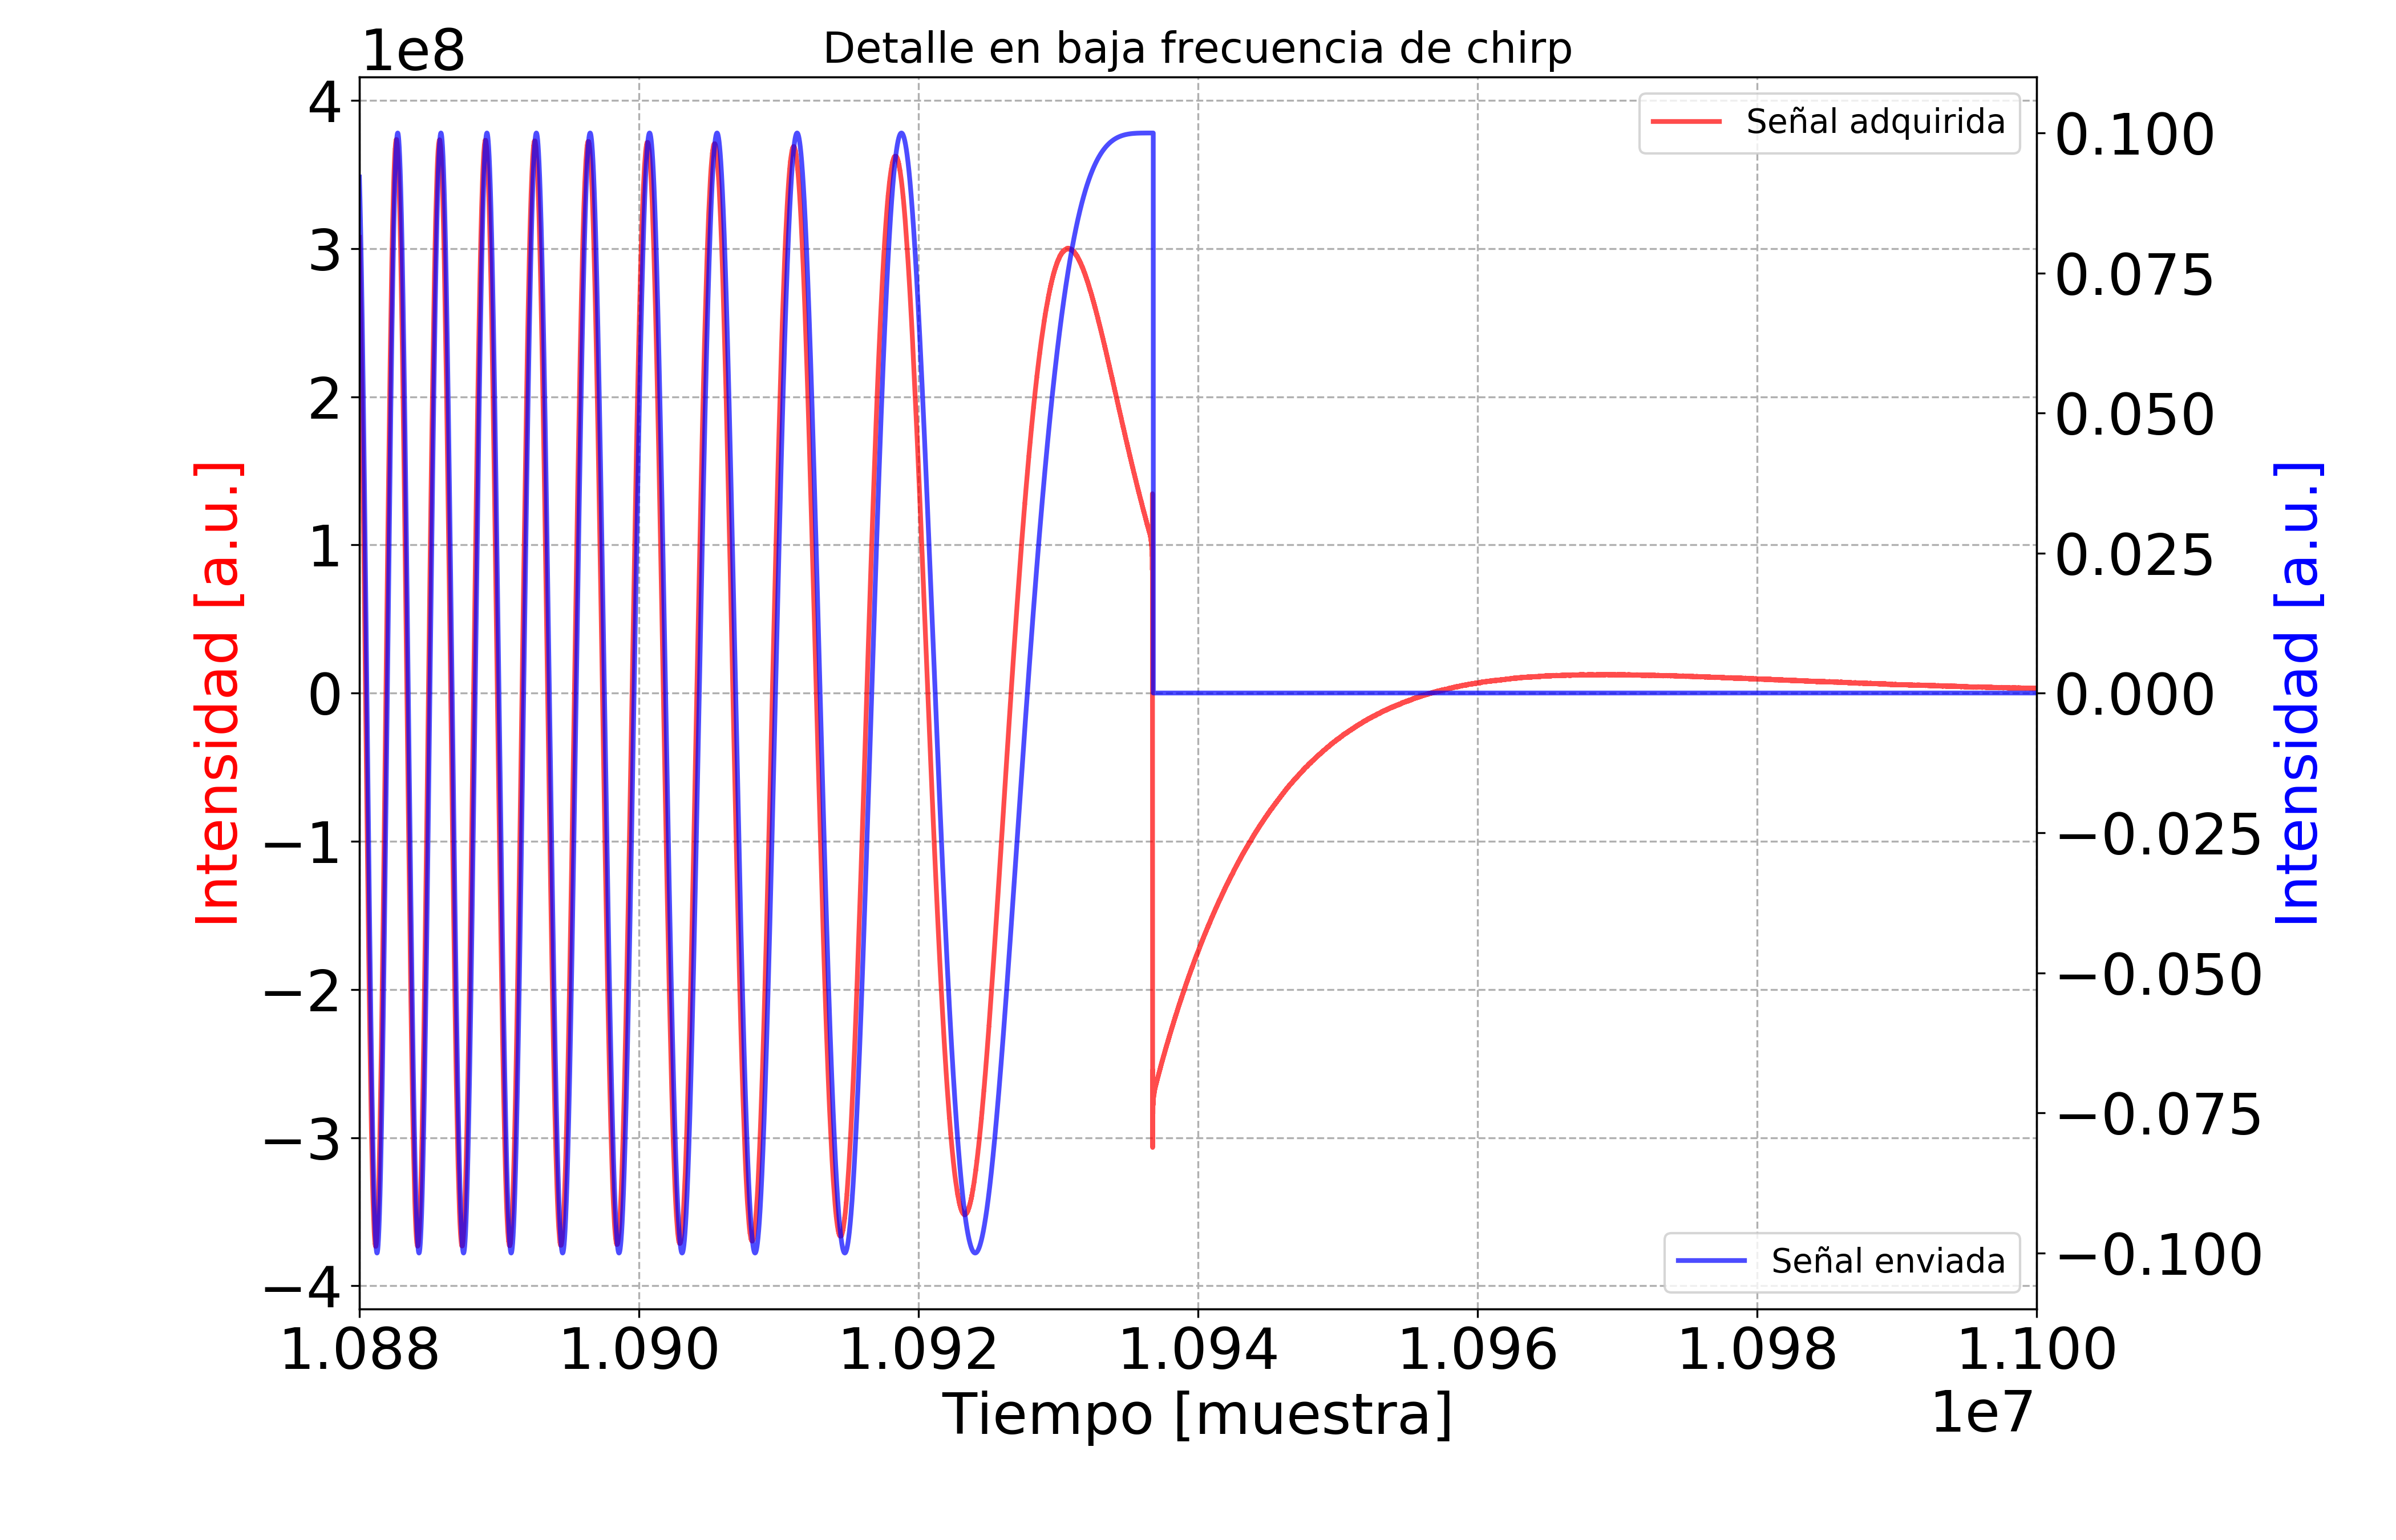
\includegraphics[scale=0.45]{chirp_baja_tiempo.png}
\caption{Detalle de seal sinusoidal con chirp enviada y adquirida con el sistema.\label{fig:chirp}}
\end{figure}
En la Figura \ref{fig:chirp_detalle} se observa el espectro en potencia de la señal digital enviada y la señal adquirida ambas normalizadas a valor correspondiente a 10000 Hz, donde la respuesta es plana. En el gráfico se observa cómo la respuesta del sistema emisor-receptor está limitada a aproximadamente 21 kHz mientras la de la señal digital llega a los 23 kHz. Si prestamos atención a las bajas frecuencias observamos un ripple en el espectro, tanto en la señal digital enviada como en la medida (Figura \ref{fig:chirp_detalle} derecha). Esto se debe a que la señal digital enviada empieza y termina con un cero de manera abrupta. Una forma de atenuar este tipo de ripple es suavizando el inicio y final de señal digital enviada. En nuestro caso decidimos normalizar la respuesta en frecuencias de la señal enviada por la esperada de la señal digital obteniendo la respuesta real (Figura \ref{fig:chirp_detalle} izquierda). De esta manera calculamos el ancho de banda del sistema a partir de los valores de frecuencia para los cuales la potencia cae a la mitad siendo de 14 Hz a 20187 Hz.

\begin{figure} [H]
\centering
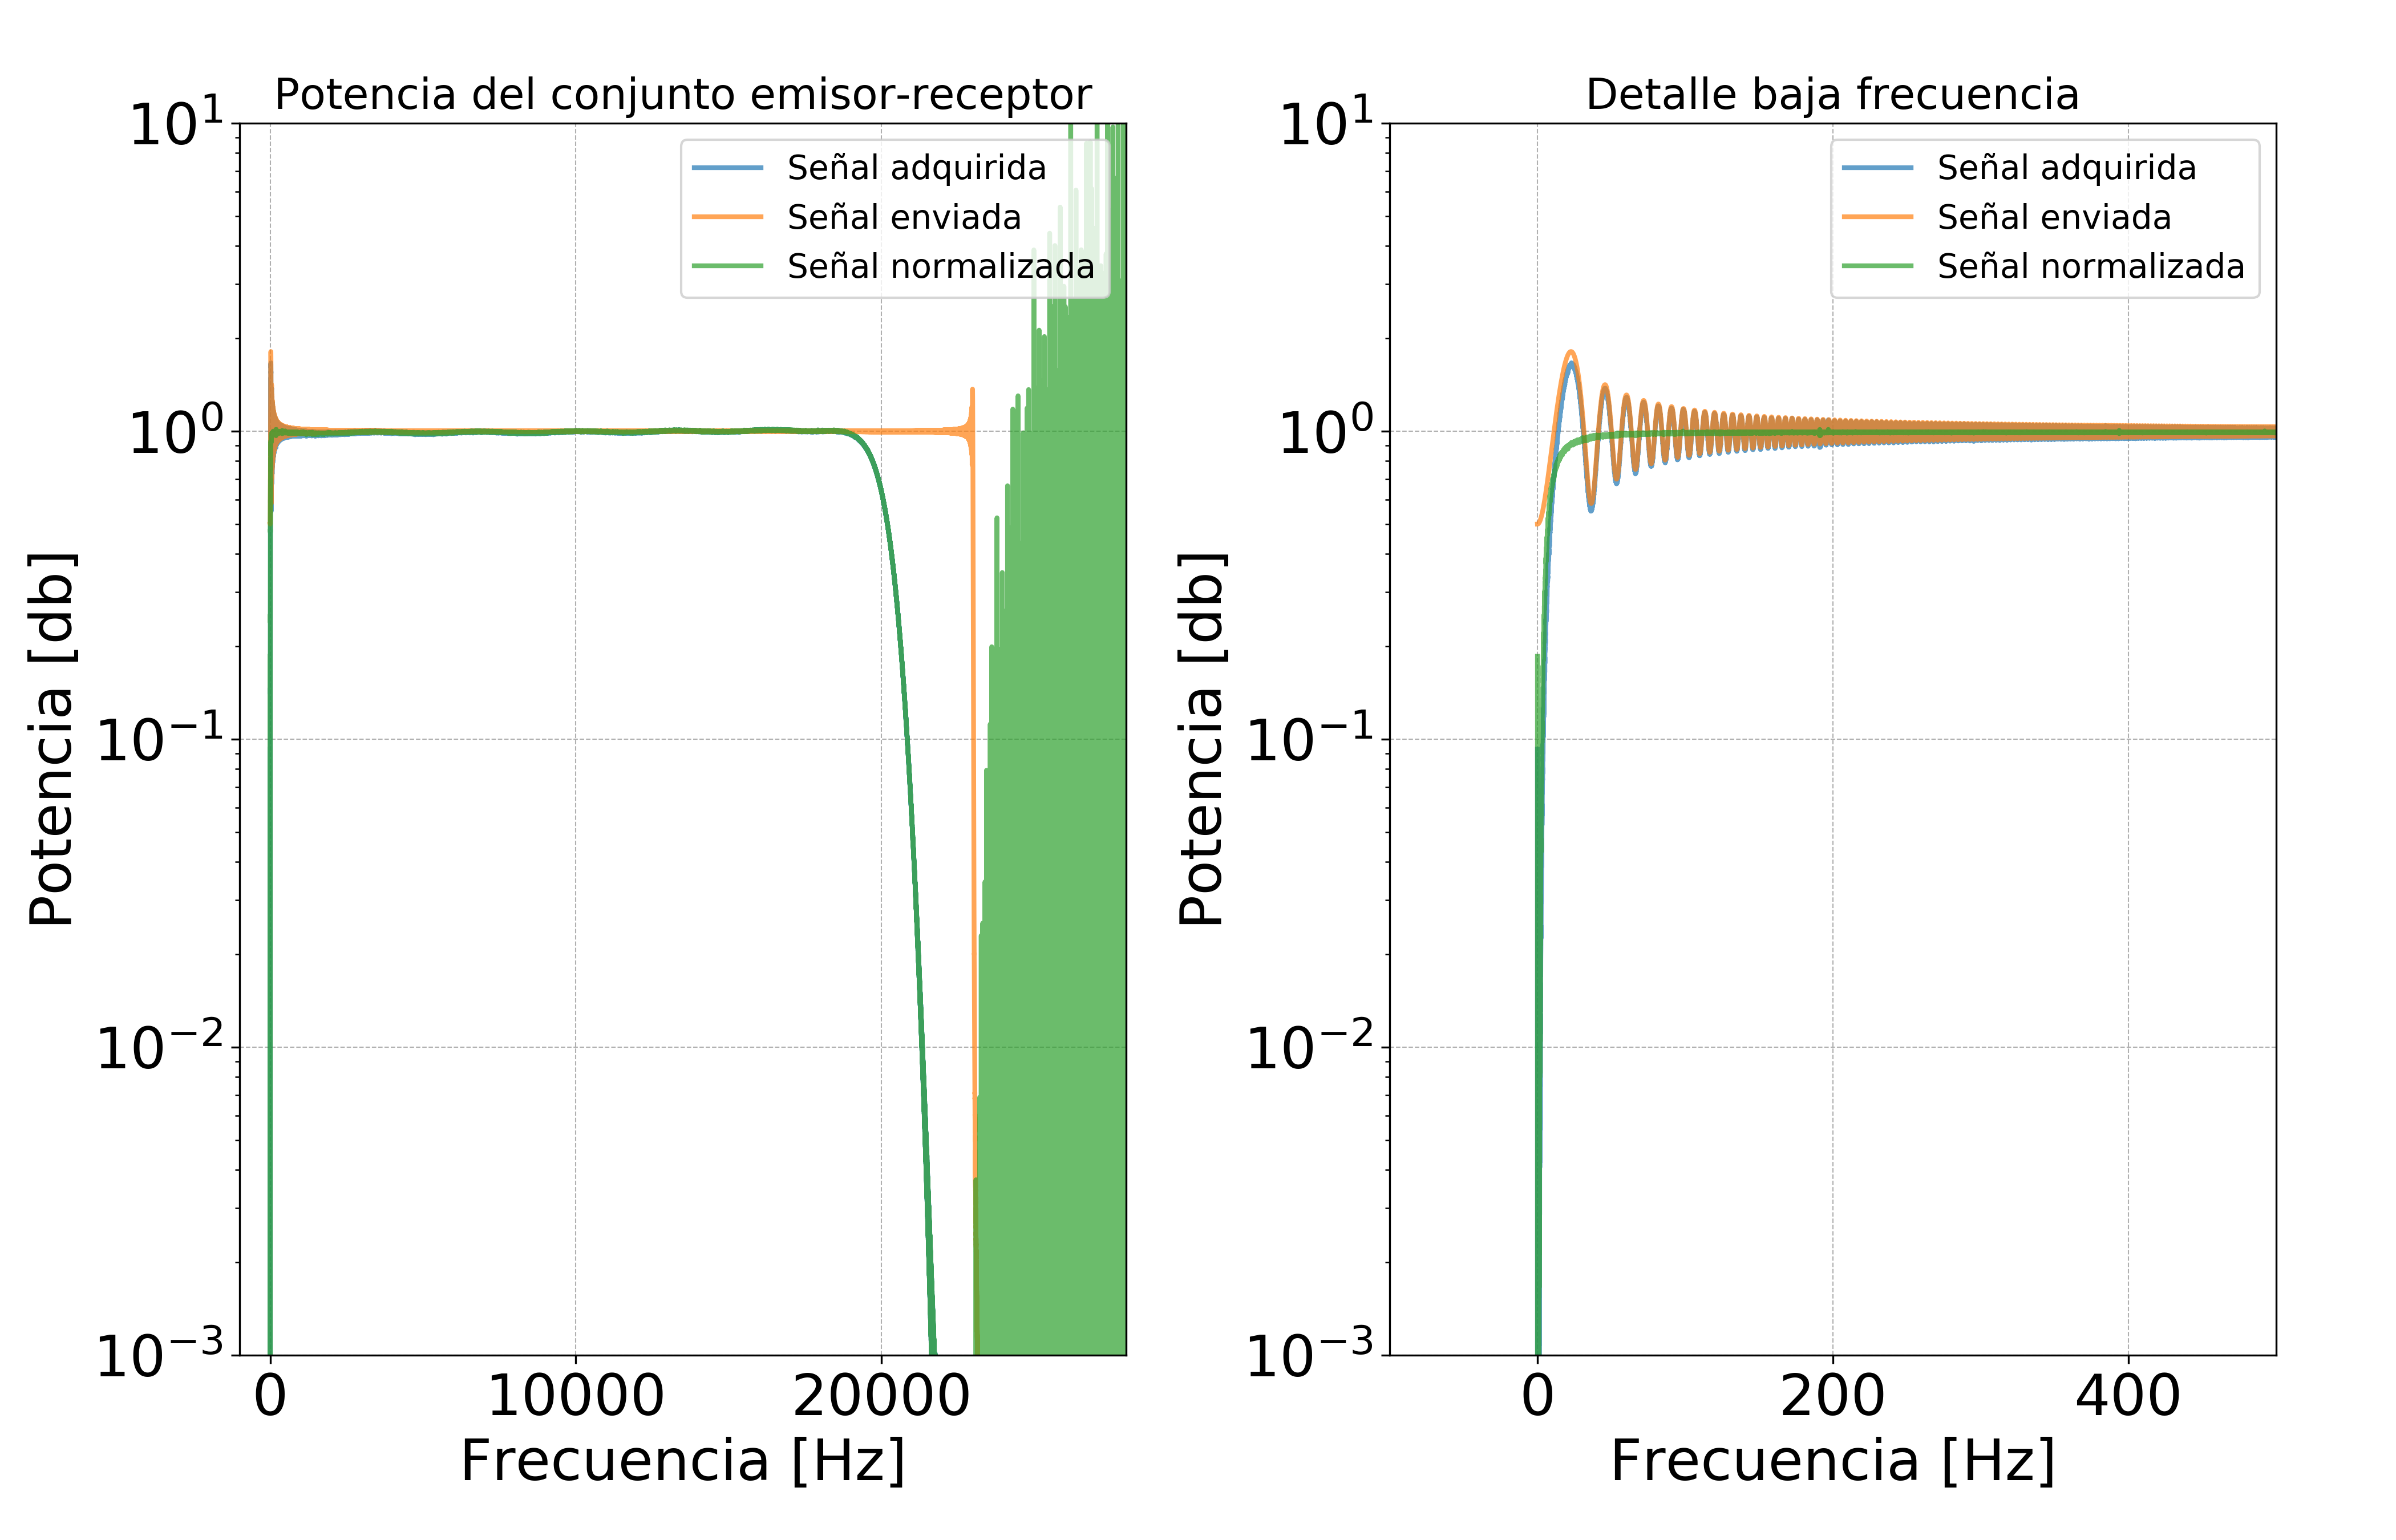
\includegraphics[scale=0.45]{chirp_detalle.png}
\caption{Izquierda. En naranja espectro del chirp enviado, en azul y verde espectro de la señal recibida antes y después de la normalización. Derecha. Detalle a baja frecuencia donde se observa ripple tanto en el espectro de la señal recibida como enviada debido al corte abrupto en el tiempo en la señal enviada y recibida. Al normalizar el espectro recibido por el enviado el ripple desaparece (verde).   \label{fig:chirp_detalle}}
\end{figure}

A modo de comparación consideramos también la respuesta en frecuencias al enviar una señal sinusoidal por cada frecuencia deseada. En la Figura \ref{fig:comparacionancho} se observan las mediciones correspondientes a los métodos de chirp y de barrido, donde se observan resultados similares. 

\begin{figure} [H]
\centering
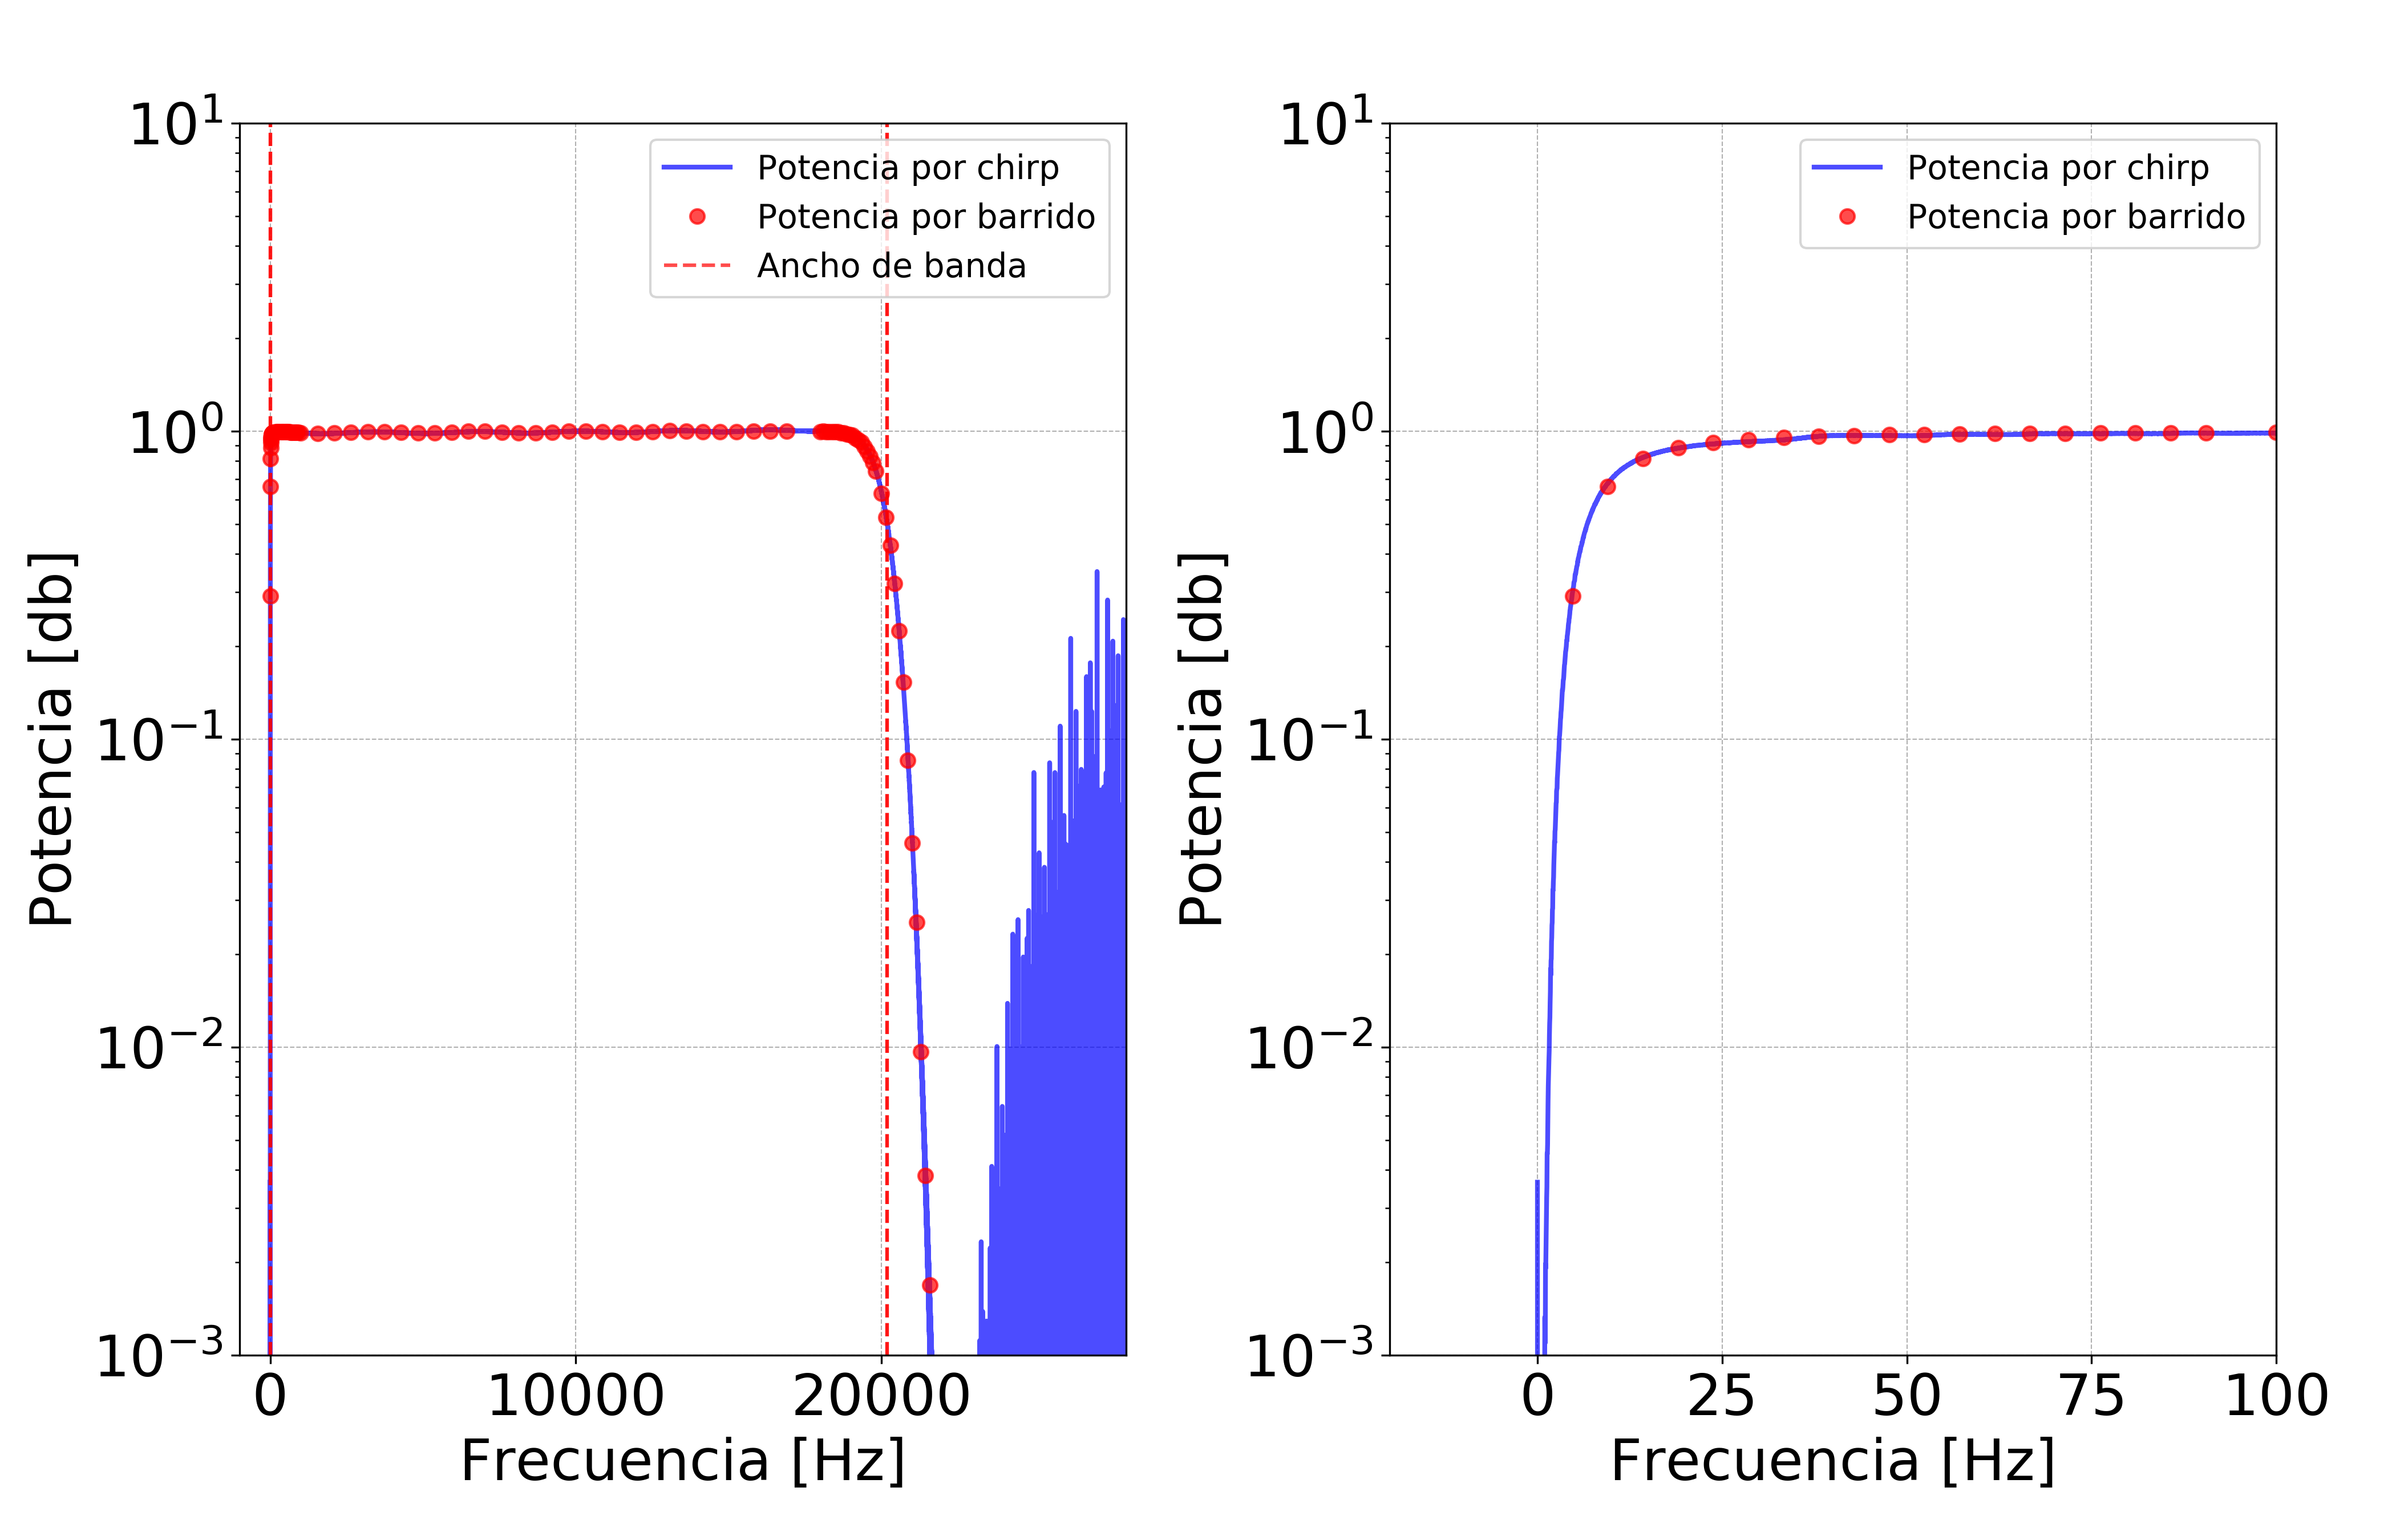
\includegraphics[scale=0.5]{comparacion_detalle.png}
\caption{Comparación entre método chirp y barrido en frecuencia para el cálculo del ancho de banda del sistema.\label{fig:comparacionancho}}
\end{figure} 

\subsection*{Calibración de canales de salida y entrada de la placa}
\subsubsection*{Parlante}
La calibración de la señal de salida (o parlante) se realizó enviando un seno de frecuencia 500 Hz en ambos canales (CH0 y CH1). Se varió el nivel del parlante de la consola de Windows 10 a la vez que se midió con un multímetro el valor de tensión RMS en modo tensión alterna. La conversión de RMS a amplitud para un seno sigue la relación:
\[
Amplitud[V]=RMS[V]{\sqrt2}
\]
La calibración se realizó con la máxima amplitud de salida posible, es decir $Amplitud_{digital}=1$. En la Figura \ref{fig:calib_parlante} se muestra la curva de amplitud en función del nivel de parlante para los canales CH0 y CH1 de salida. Y la máxima tensión de salida es de 3.2 V para un nivel de parlante 100/100.

\begin{figure} [H]
\centering
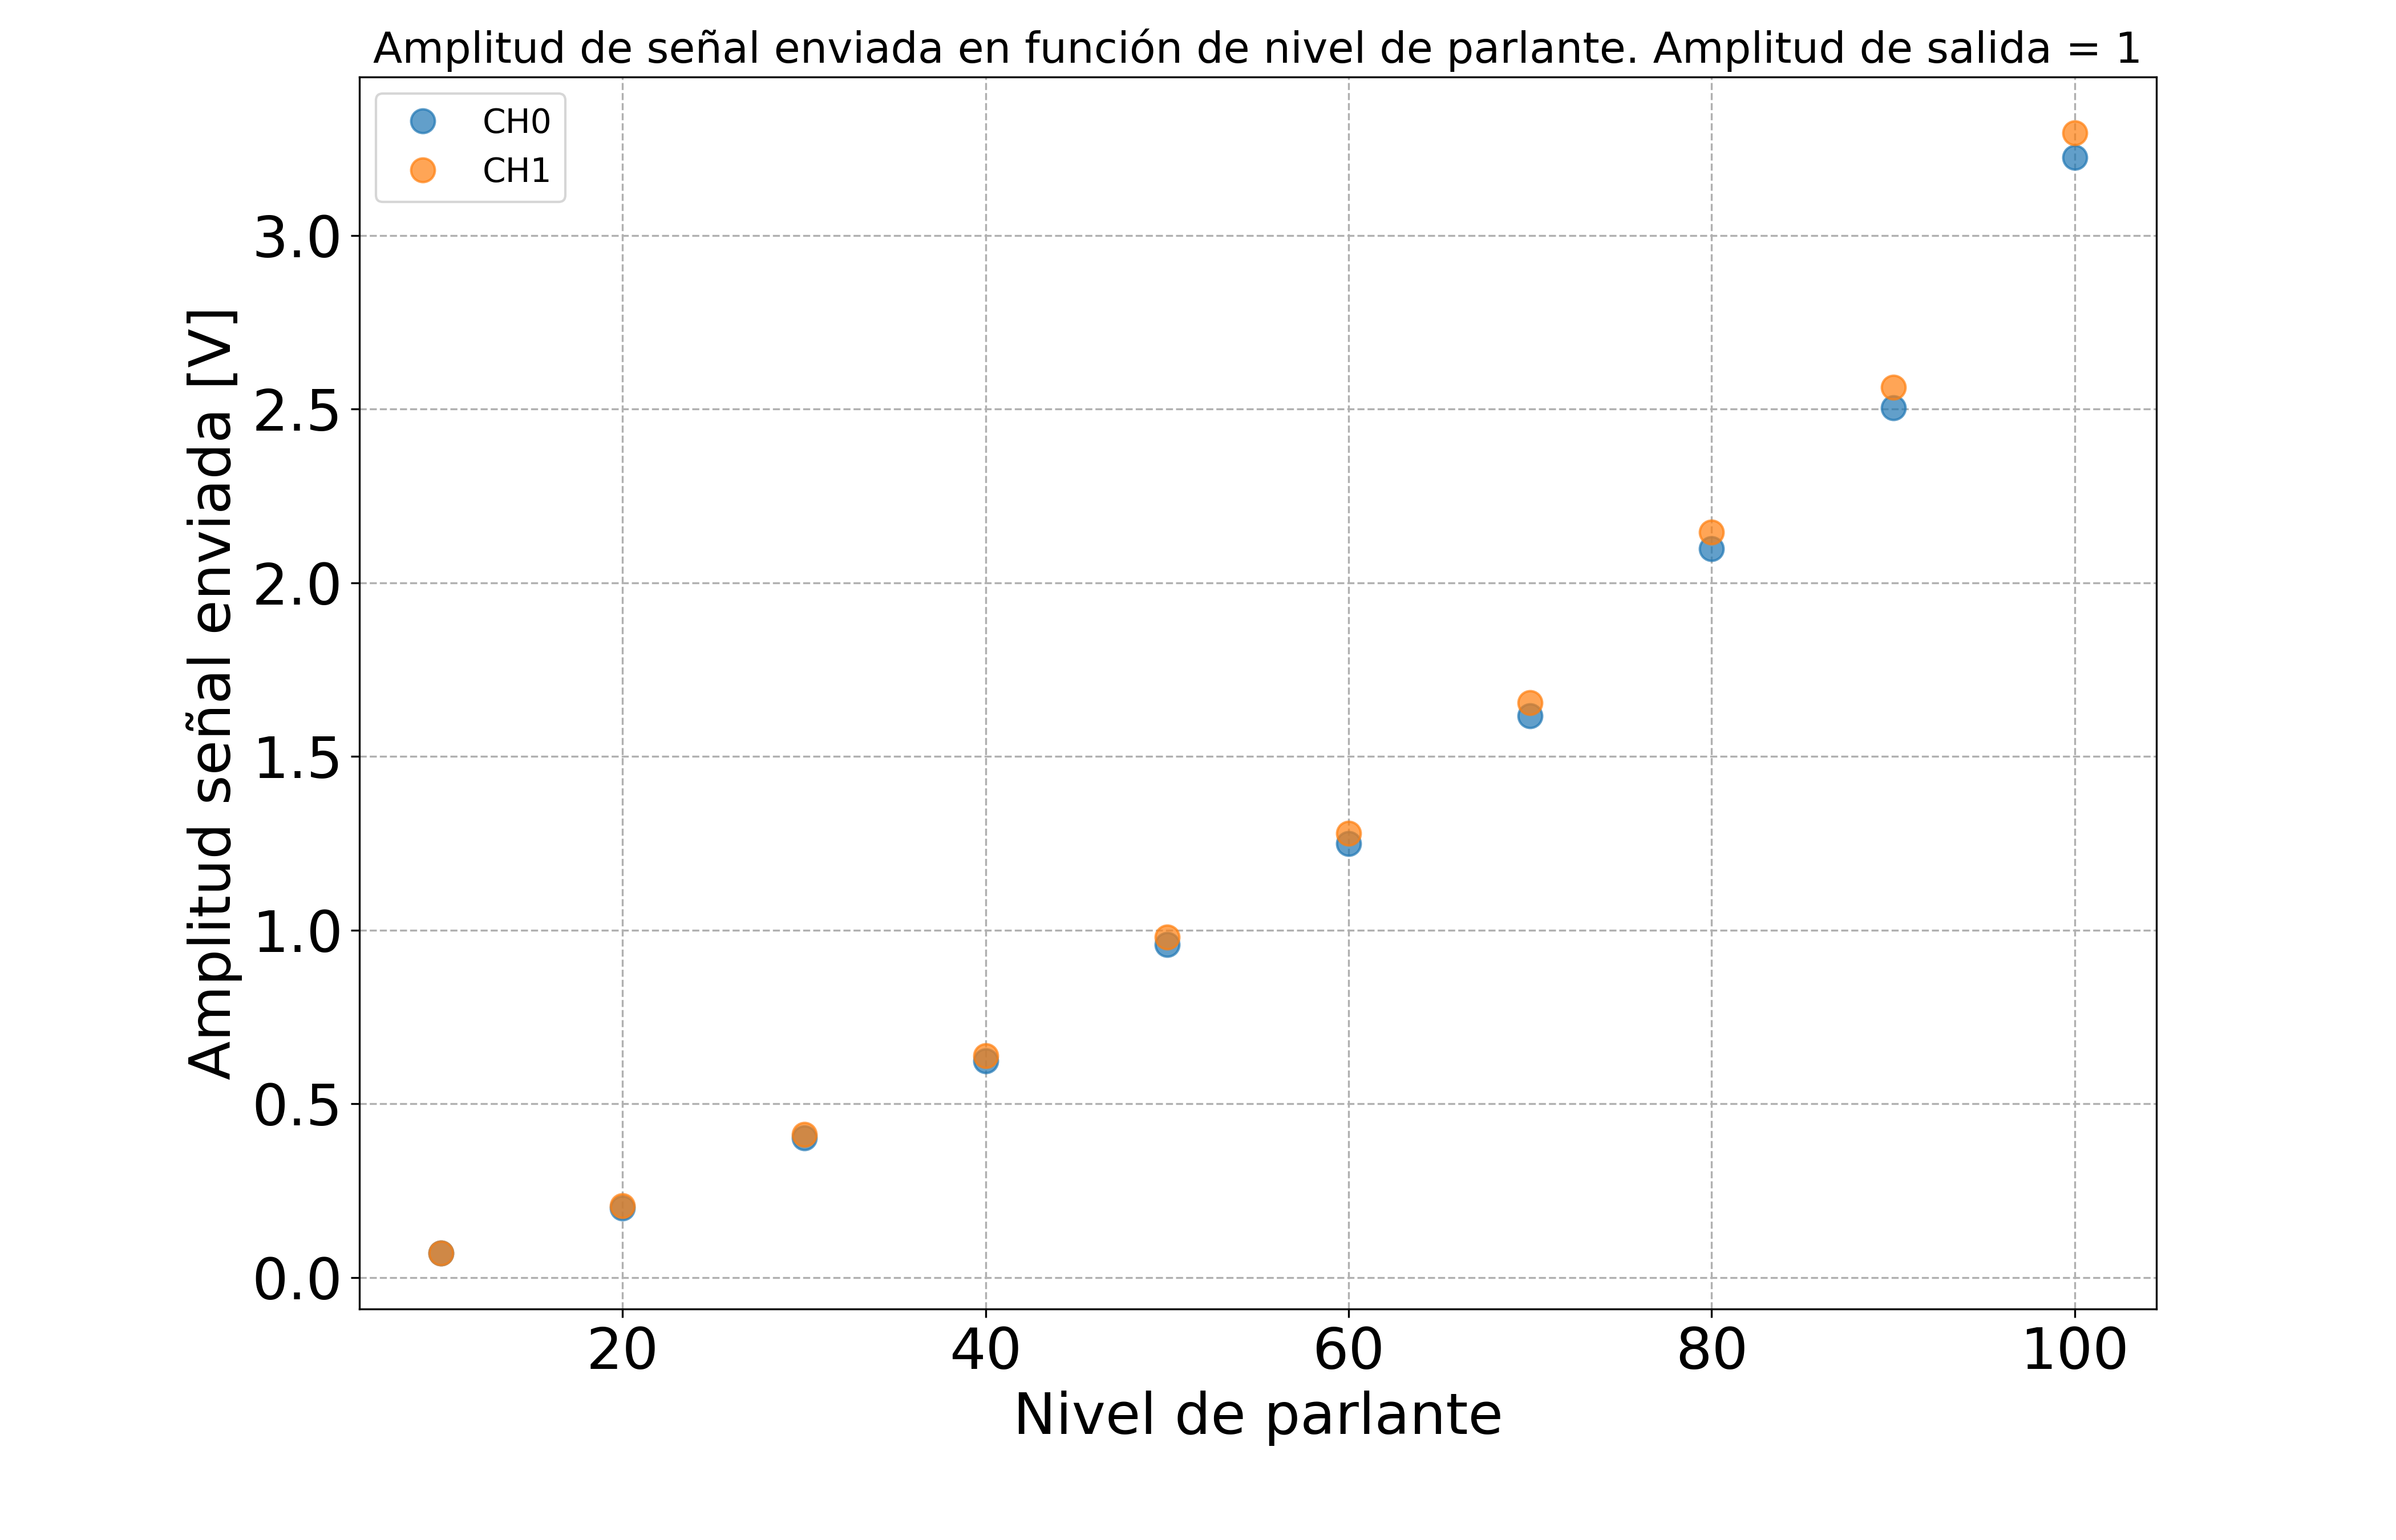
\includegraphics[scale=0.45]{respuesta_por_nivel_parlante.png}
\caption{Amplitud de tensión de salida en función del nivel de parlante.\label{fig:calib_parlante}}
\end{figure} 

\subsubsection*{Micrófono}
Para la calibración del micrófono se envió una señal de tipo de seno de frecuencia 1 kHz y amplitud constante 0.4 V, y se varió el nivel de micrófono de la consola de Windows. En la Figura \ref{fig:calibmic} se muestran las rectas de calibración para los distintos niveles de micrófono. El tipo de dato de entrada es un entero de 16 bits por lo que el rango en cuentas queda determinado por los valores[$-2^{15}$,$2^{15}$] es decir [-32767,+ 32768]. Una vez que se supera el rango la medición satura. Cabe destacar que la placa admite la adquisición en enteros de 32 bits, pero esto no significa mayor resolución pues los valores posibles están distanciados siempre por $2^{16}$  cuentas.
En la Figura \ref{fig:ejemplo_rangomic} se muestra un ejemplo de señal enviada y adquirida, y su correspondiente ajuste al utilizar un nivel de micrófono 100/100. Por lo tanto si obtenemos un ajuste lineal de tipo:
\[
senal[cuentas]=a_{mic}*senal [V]+b_{mic}
\]
La conversión en tensión de la señal adquirida queda entonces:
\[
senal [V]=\frac{senal[cuentas]-b_{mic}}{a_{mic}}
\]
Del gráfico se comprueba además la respuesta lineal de la entrada.
Utilizando la calibración para cada nivel de micrófono podemos determinar su rango teórico en tensión. En la Figura \ref{fig:calib_microfono} se muestra el nivel del rango positivo en función del nivel de micrófono, donde se observa un rango teórico máximo de hasta $\pm$30 V para un valor de nivel de micrófono de 10/100, obtenido a partir de la calibración mostrarda arriba según la relación: 
\[
rango_{mic} [V]=\frac{2^{15}}{a_{mic}}
\]
Luego se comprobó que el rango de la entrada está limitado en aproximadamente $\pm$ 2.10 V.

\begin{figure}[H]
        \begin{subfigure}[b]{0.5\textwidth}
                \centering
                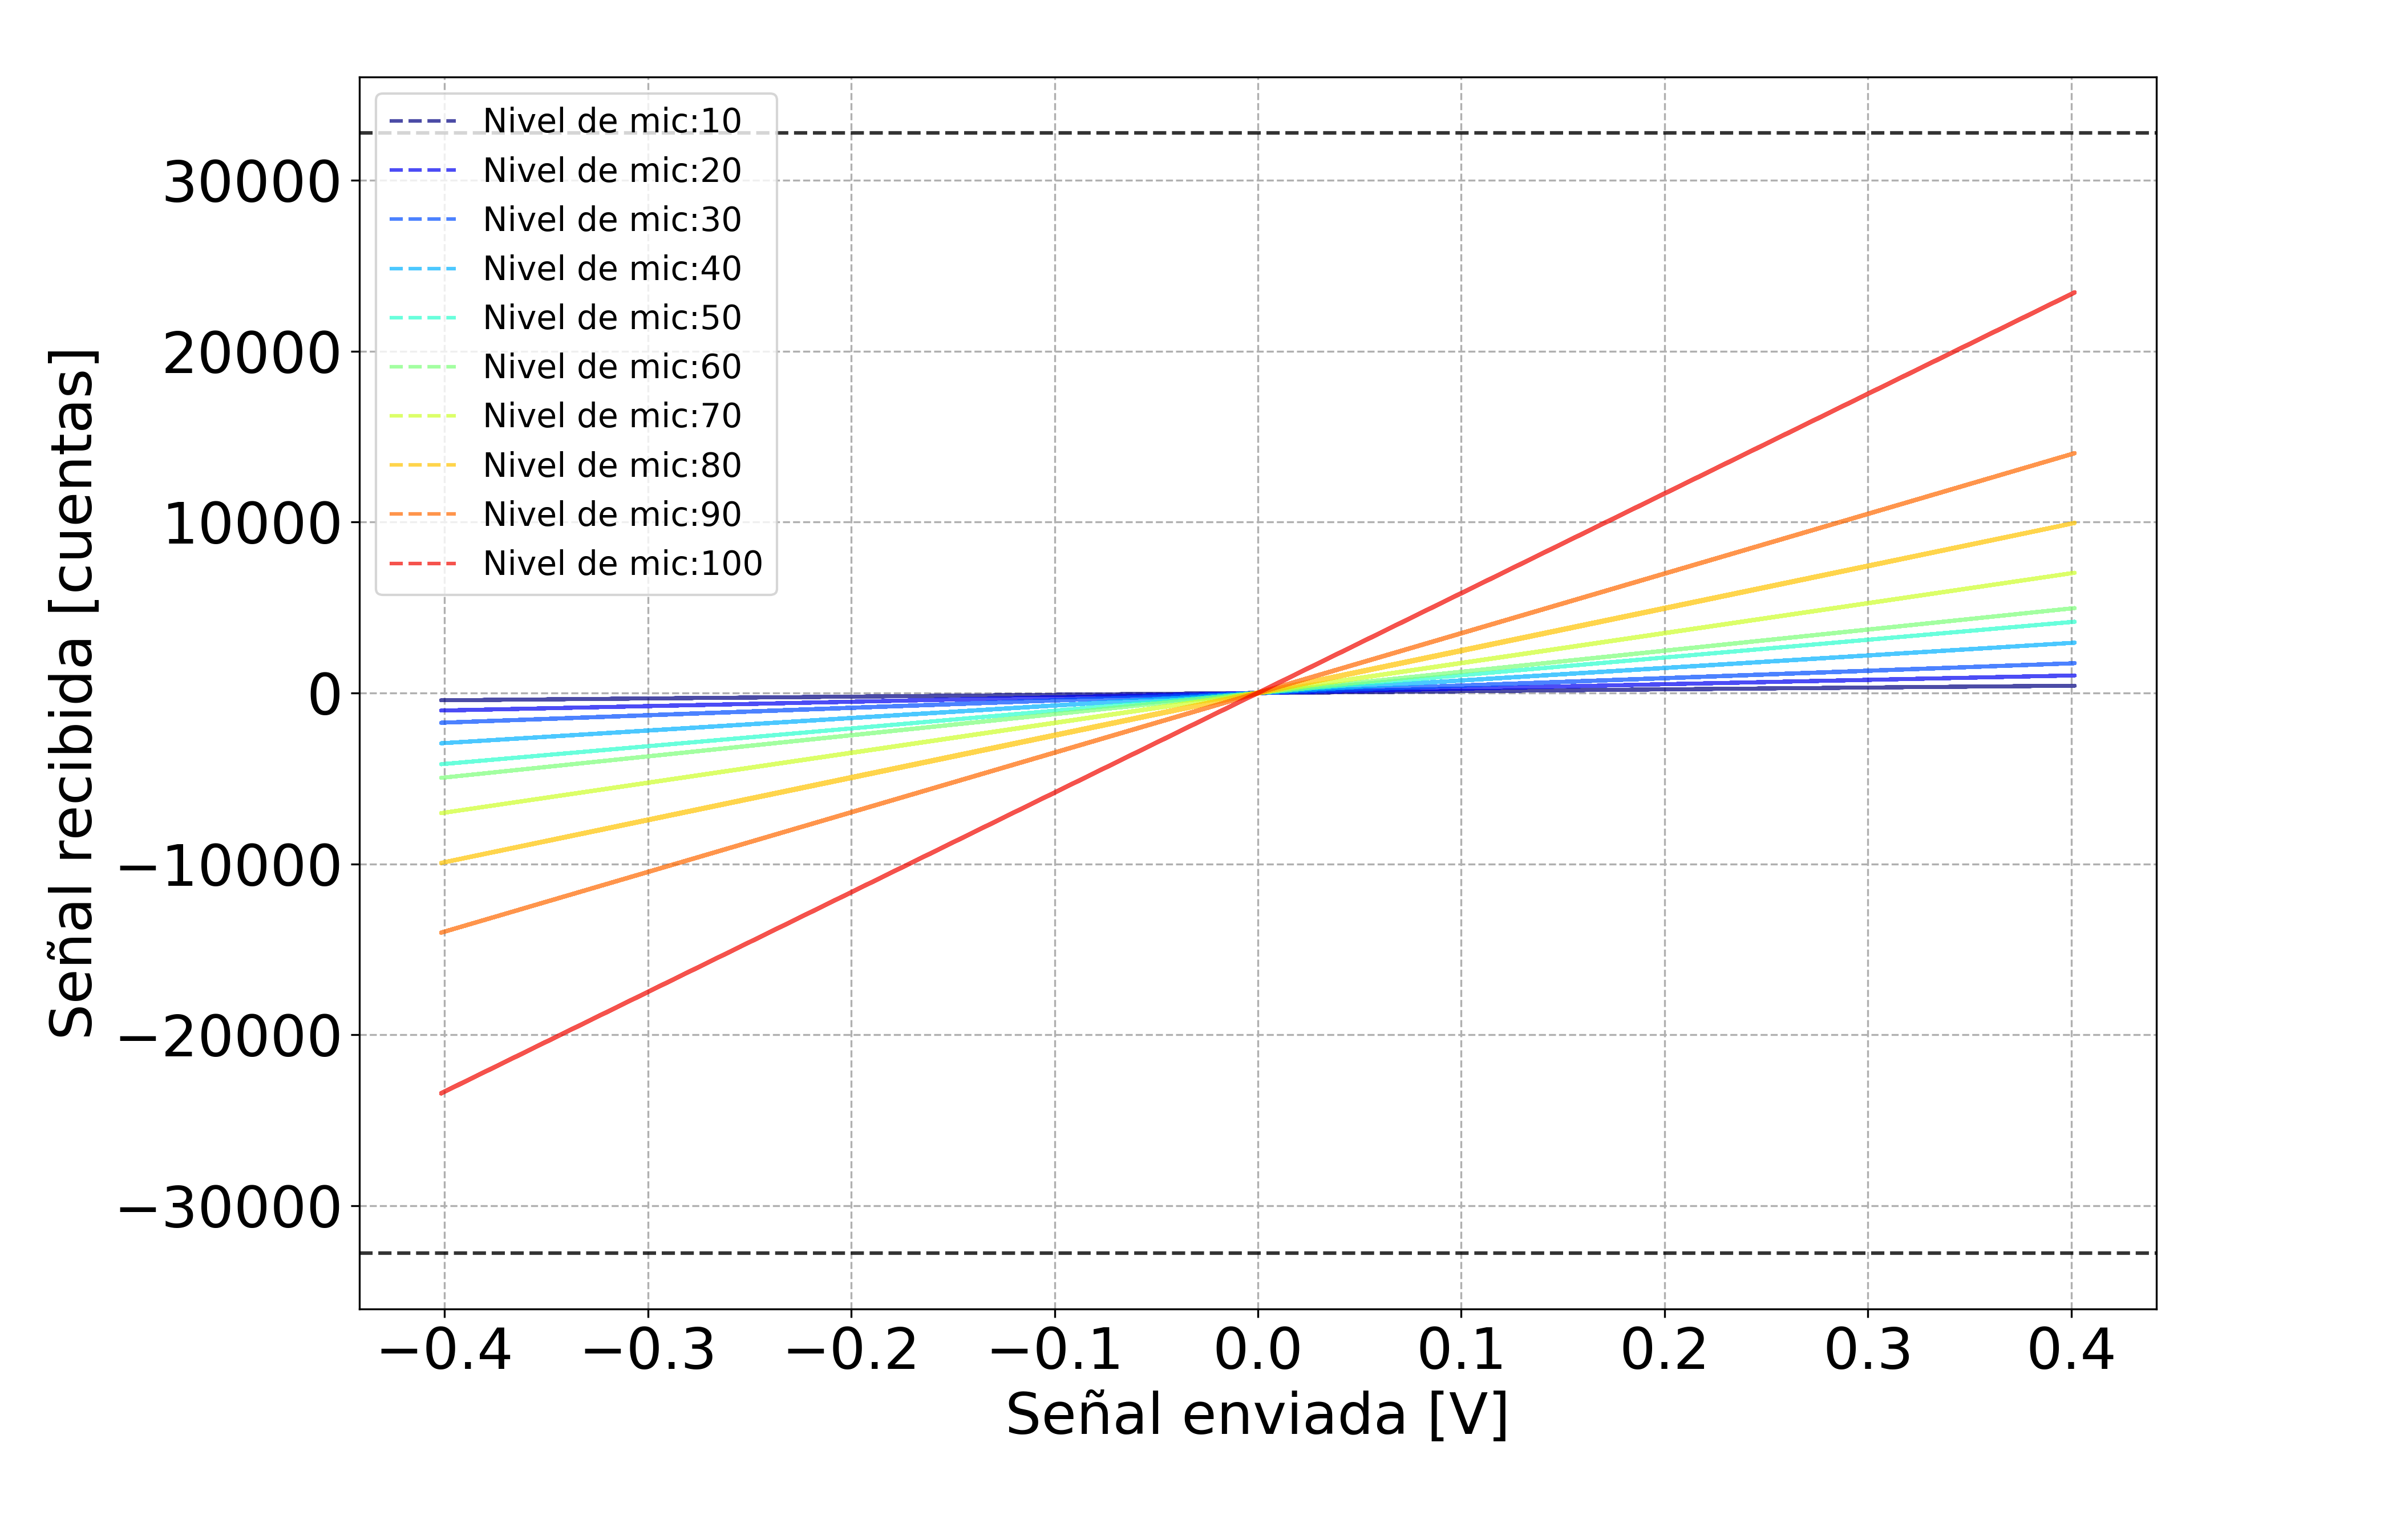
\includegraphics[width=\linewidth]{respuesta_por_nivel_mic.png}
                \caption{} \label{fig:calibmic}
        \end{subfigure}%
        \begin{subfigure}[b]{0.5\textwidth}
                \centering
                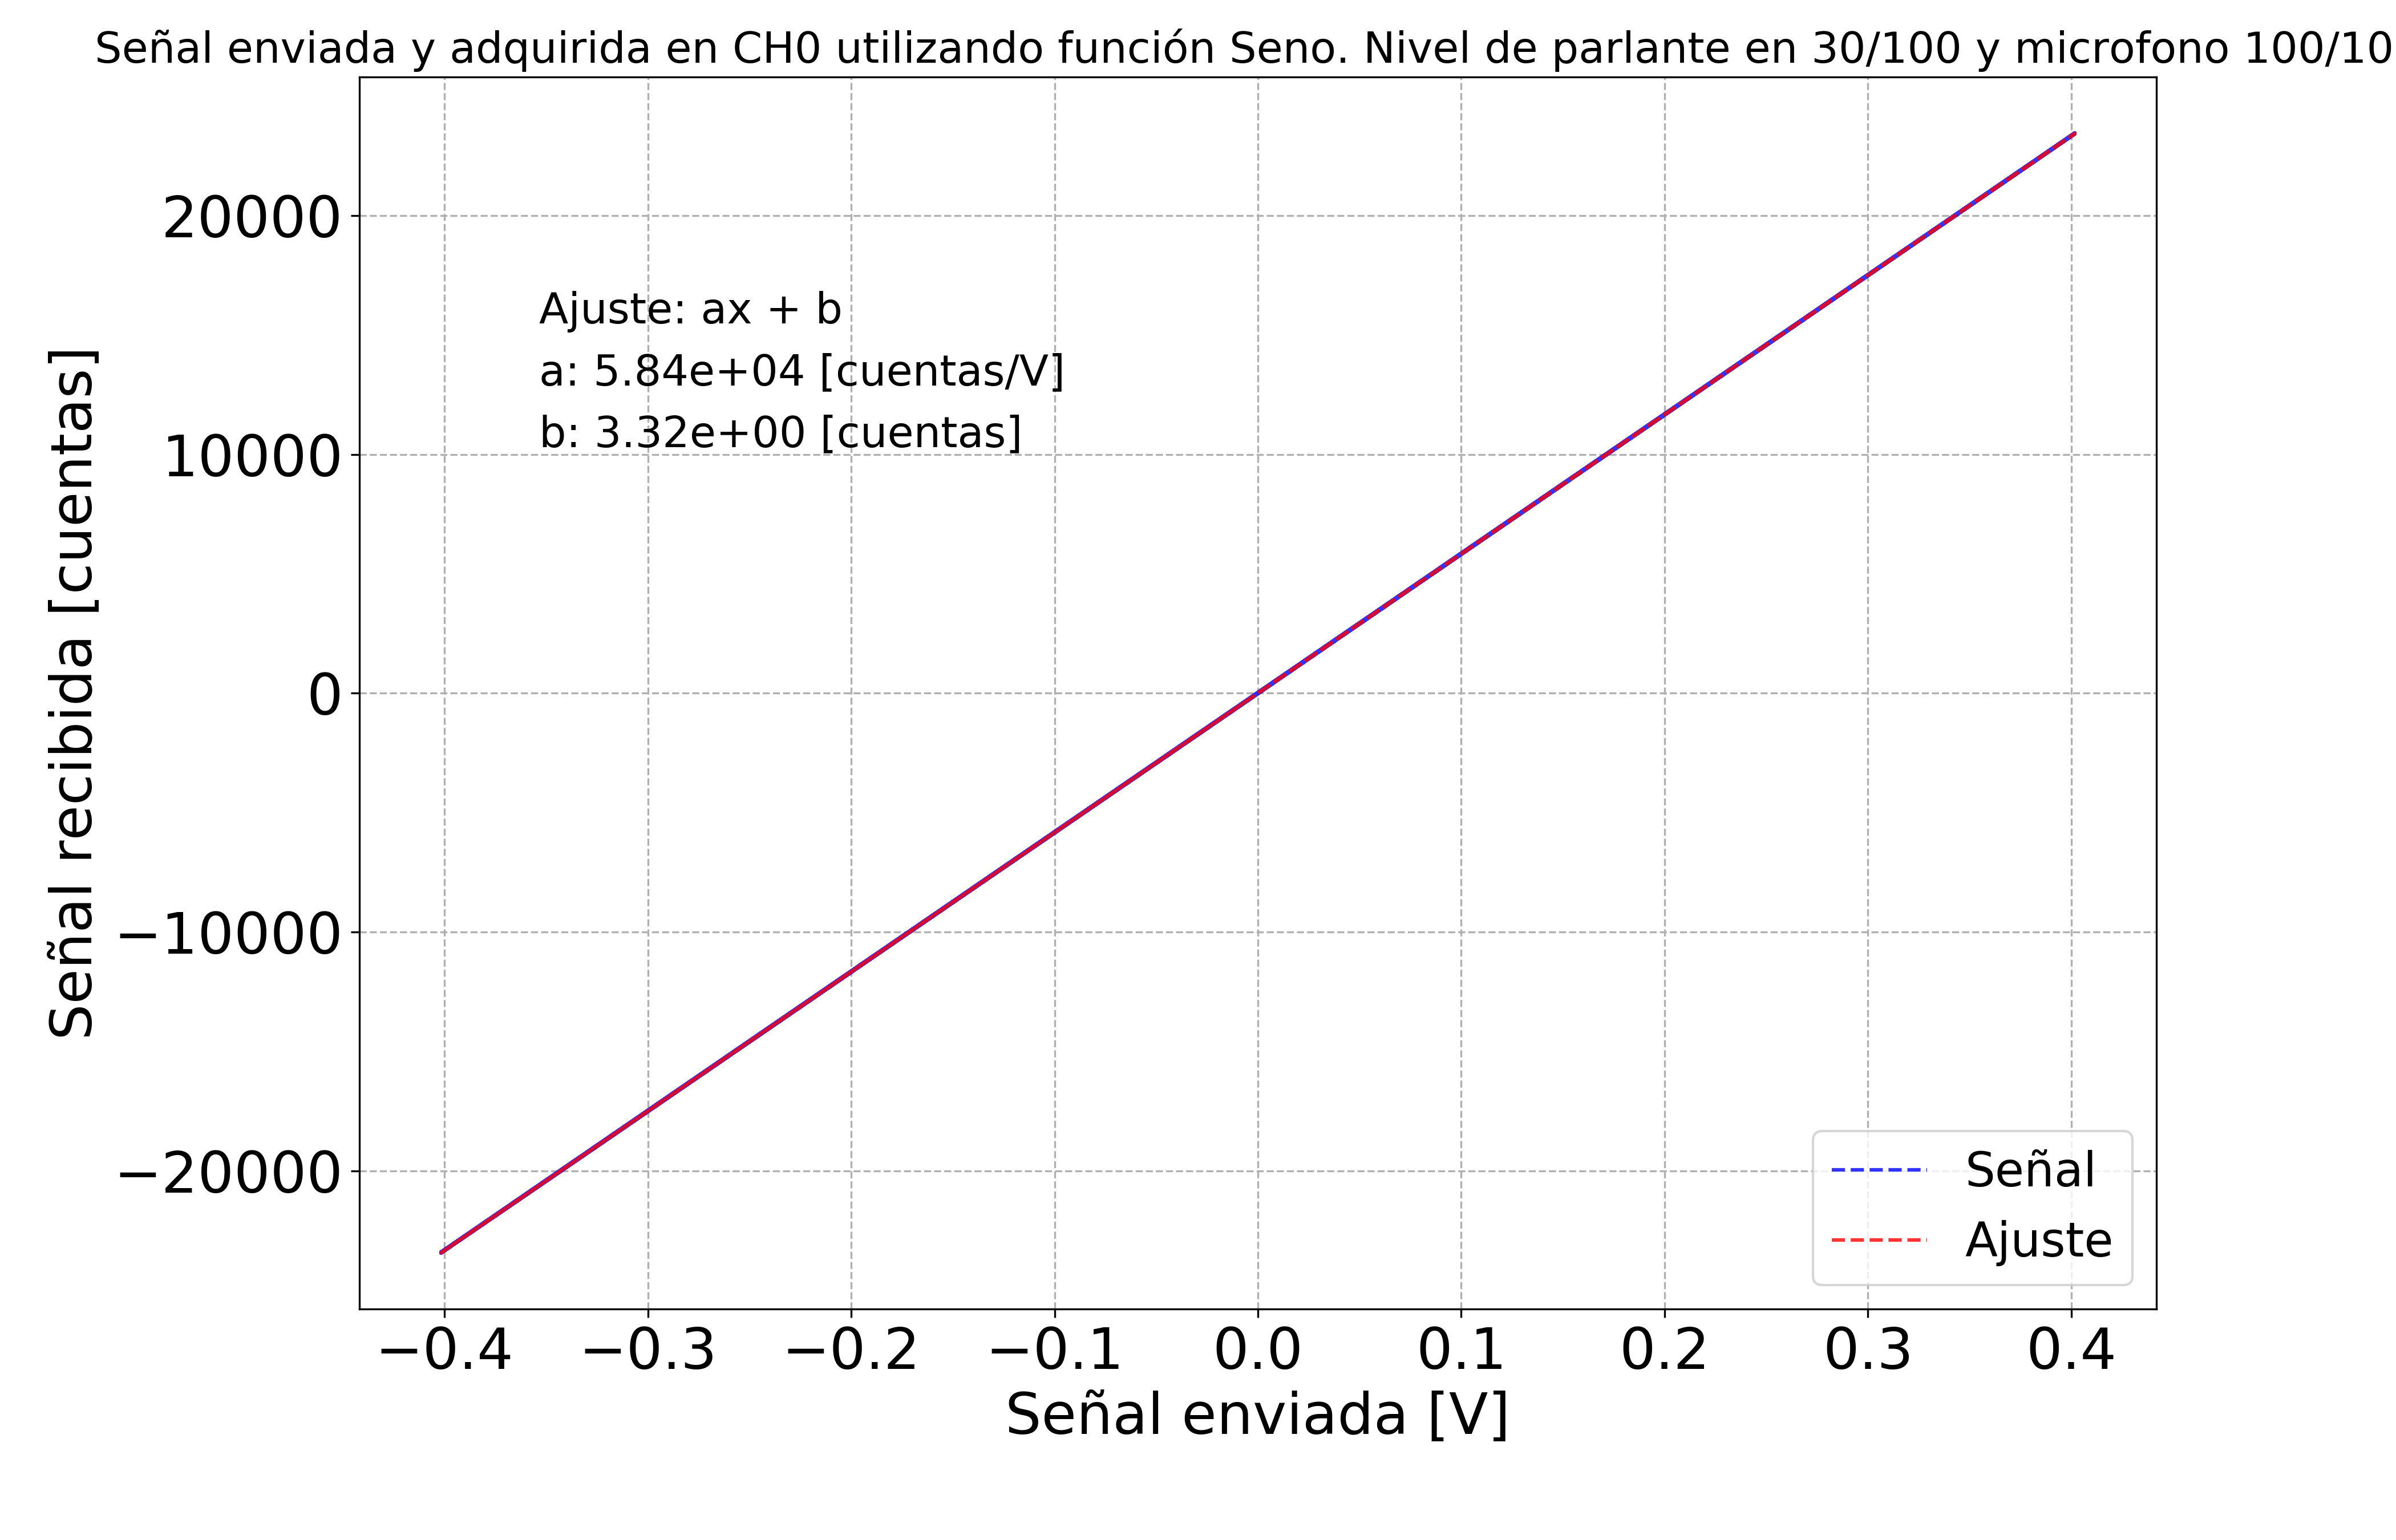
\includegraphics[width=\linewidth]{ajuste_CH0_Seno_wm100_int16.png}
                \caption{} \label{fig:ejemplo_rangomic}
        \end{subfigure}%
        \caption{a) Señal adquirida vs. señal enviada para distintos niveles de micrófono al enviar un seno de amplitud constante. b) Detalle de señal y ajuste lineal para nivel de micrófono 100/100.}\label{fig:calib_microfono}
\end{figure}

\begin{figure} [H]
\centering
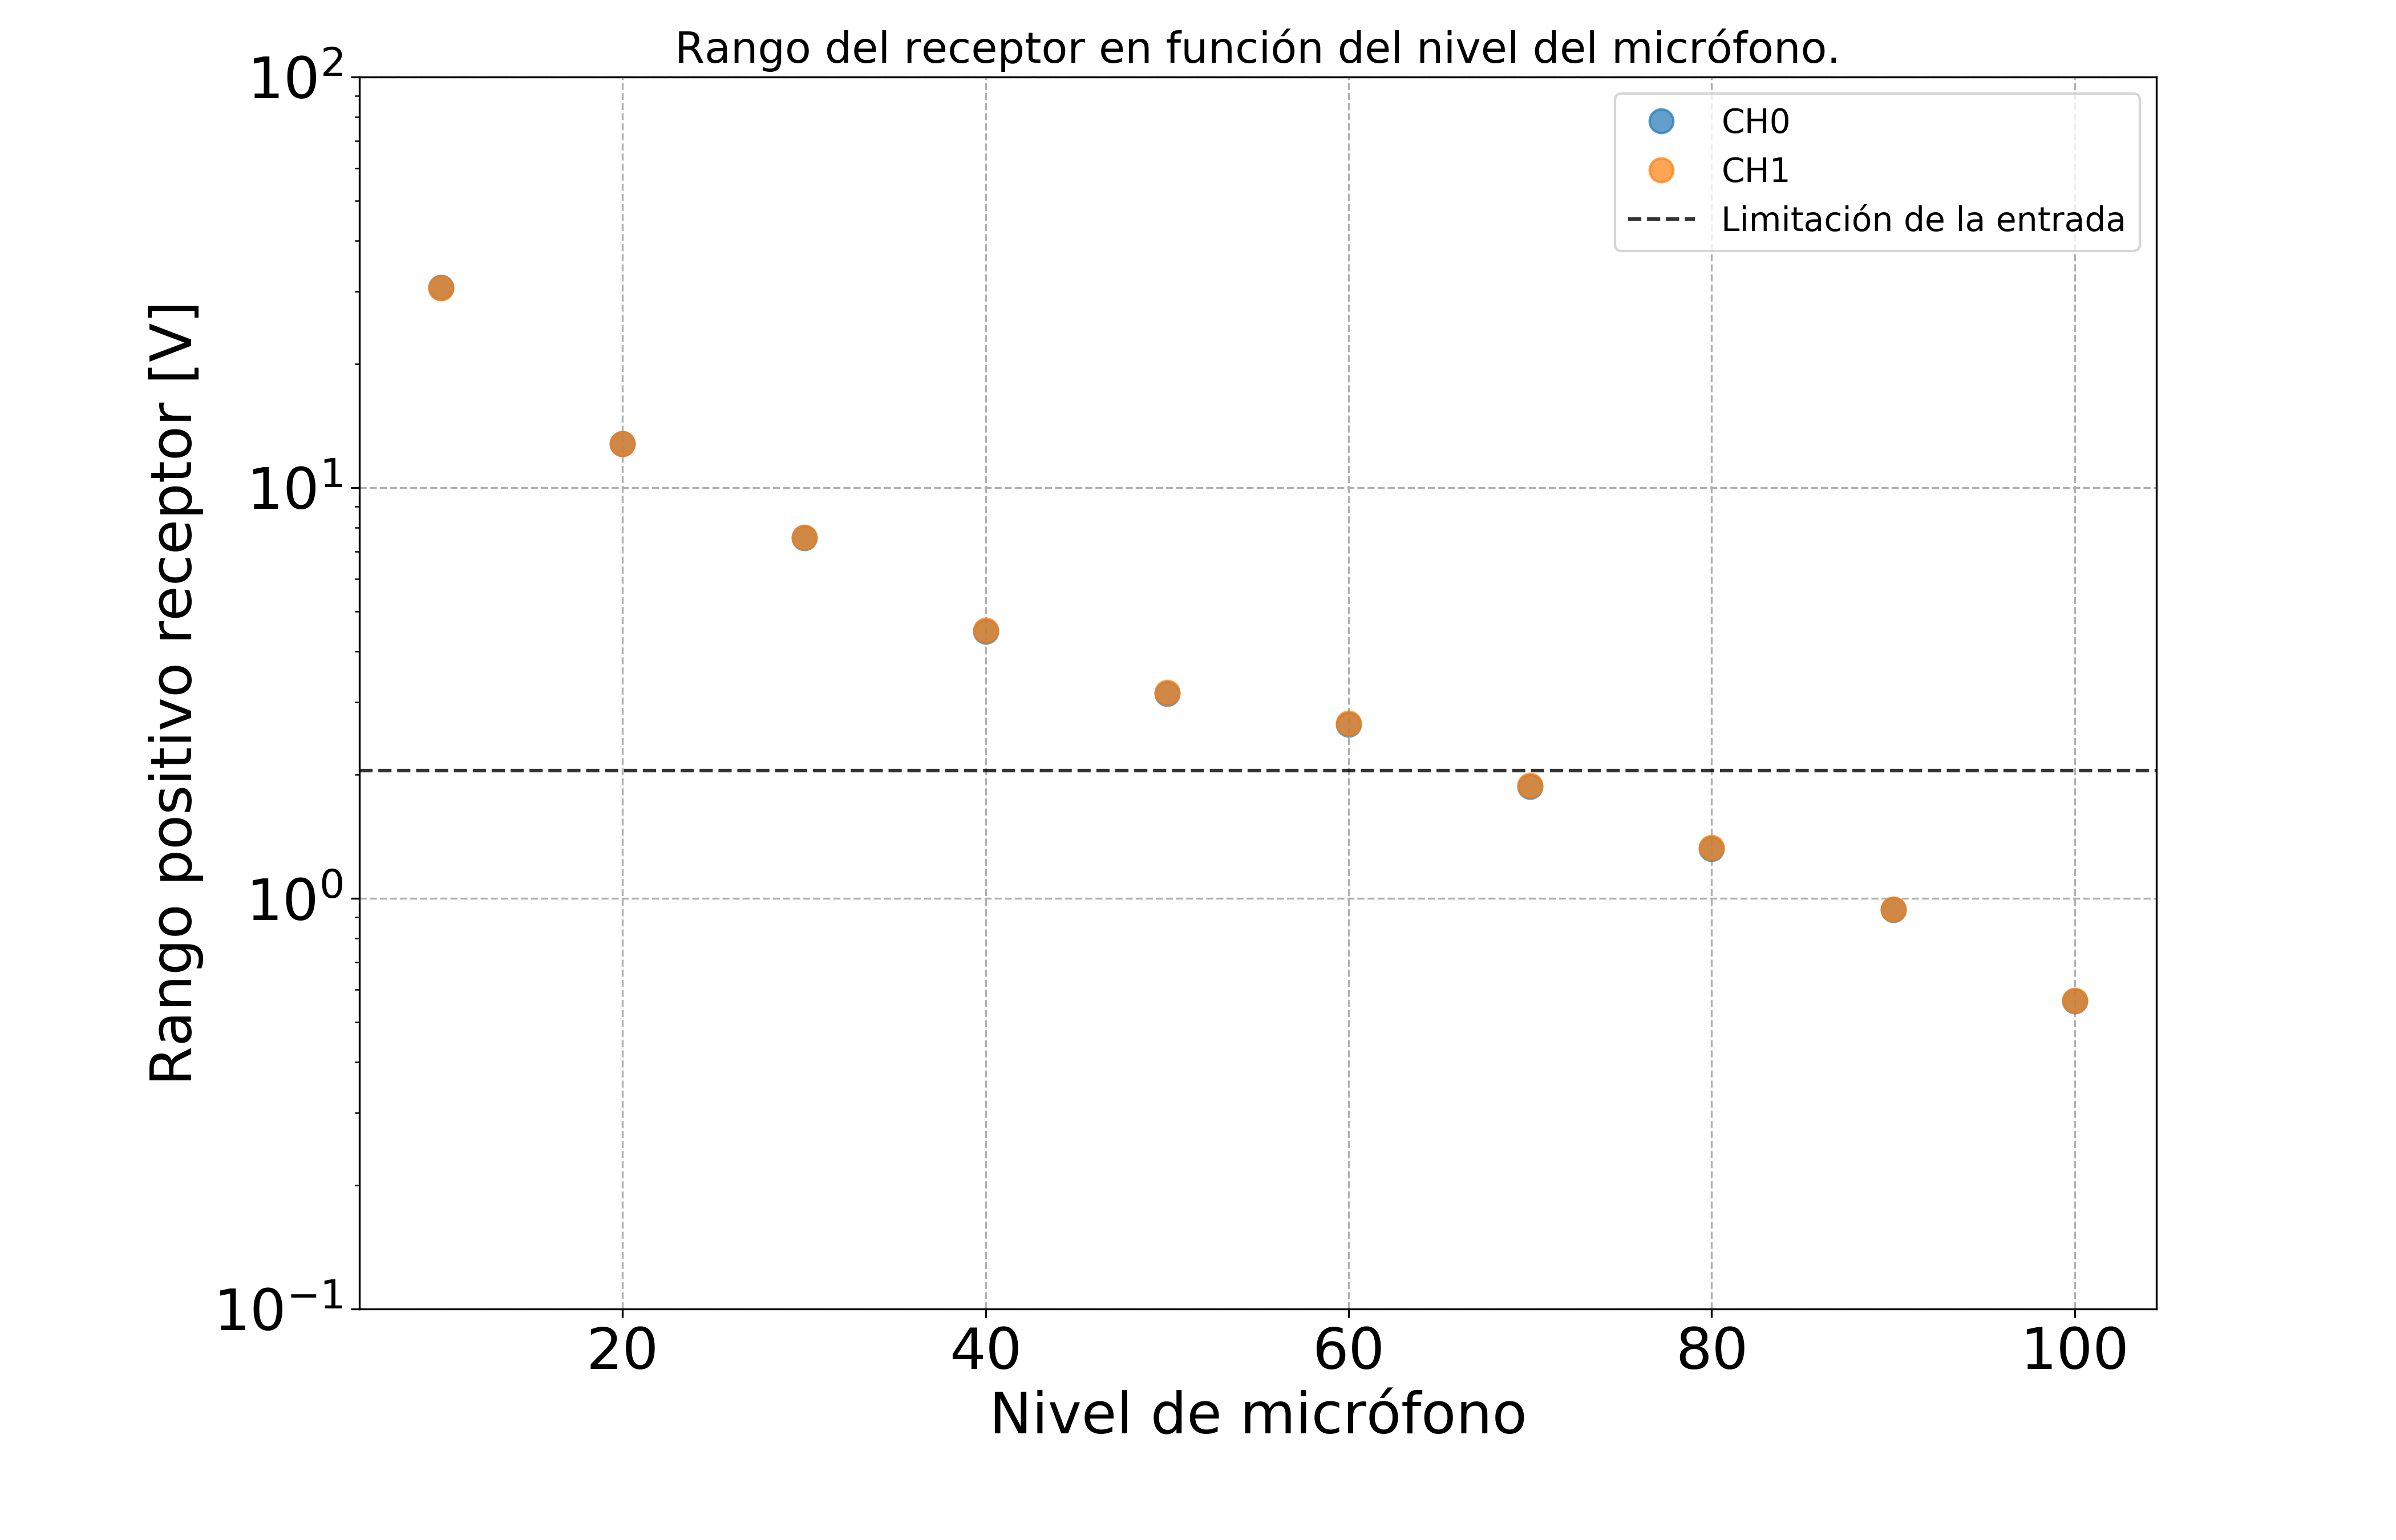
\includegraphics[scale=0.45]{respuesta_por_nivel_microfono_rango.png}
\caption{Rango positivo de tensión de entrada en función del nivel de micrófono.\label{fig:calib_microfono}}
\end{figure} 

 En la Tabla 1 mostramos la calibración para cada nivel de micrófono:

\begin {table}[H]
\begin {center}
 \begin{tabular} {|c|c|}
        \hline
        Nivel de micrófono &  1/a  $[\mu V/cuenta]$ \\
        \hline
        10/100 & 939\\
        \hline
        20/100 & 391\\
        \hline
        30/100 & 231\\
        \hline
        40/100 & 136\\
        \hline
        50/100 & 96.3\\
        \hline
        60/100 & 80.9\\
        \hline
        70/100 & 57.1\\
        \hline
        80/100 & 40.3\\
        \hline
        90/100 & 28.6\\
        \hline
        100/100 & 17.1\\
        % \hline
        % ADSDASD & ADASDAD\\
        \hline
 \end{tabular}
 \caption{Calibración de la entrada de la placa de audio en función del nivel del micrófono}
 \label{table1}
 \end{center}
\end{table}

\subsection*{Ruido}
A continuación medimos los niveles de ruido de la placa al medir un cero (o tierra) en ambos canales de entrada. Cabe destacar que al hacer esto estamos considerando todas las fuentes de ruido posibles como ser ruido de digitalización, lectura, ruido de temperatura (o ancho de banda) del circuito de entrada y ruido de la tierra.  En la Figura \ref{fig:ruidocuentas} se muestra el histograma de ruido en tensión y cuentas para un nivel de micrófono de 50/100. Dado que la distribución es gaussiana consideramos la desviación estándar (STD) como medida del ruido.
\begin{figure} [H]
\centering
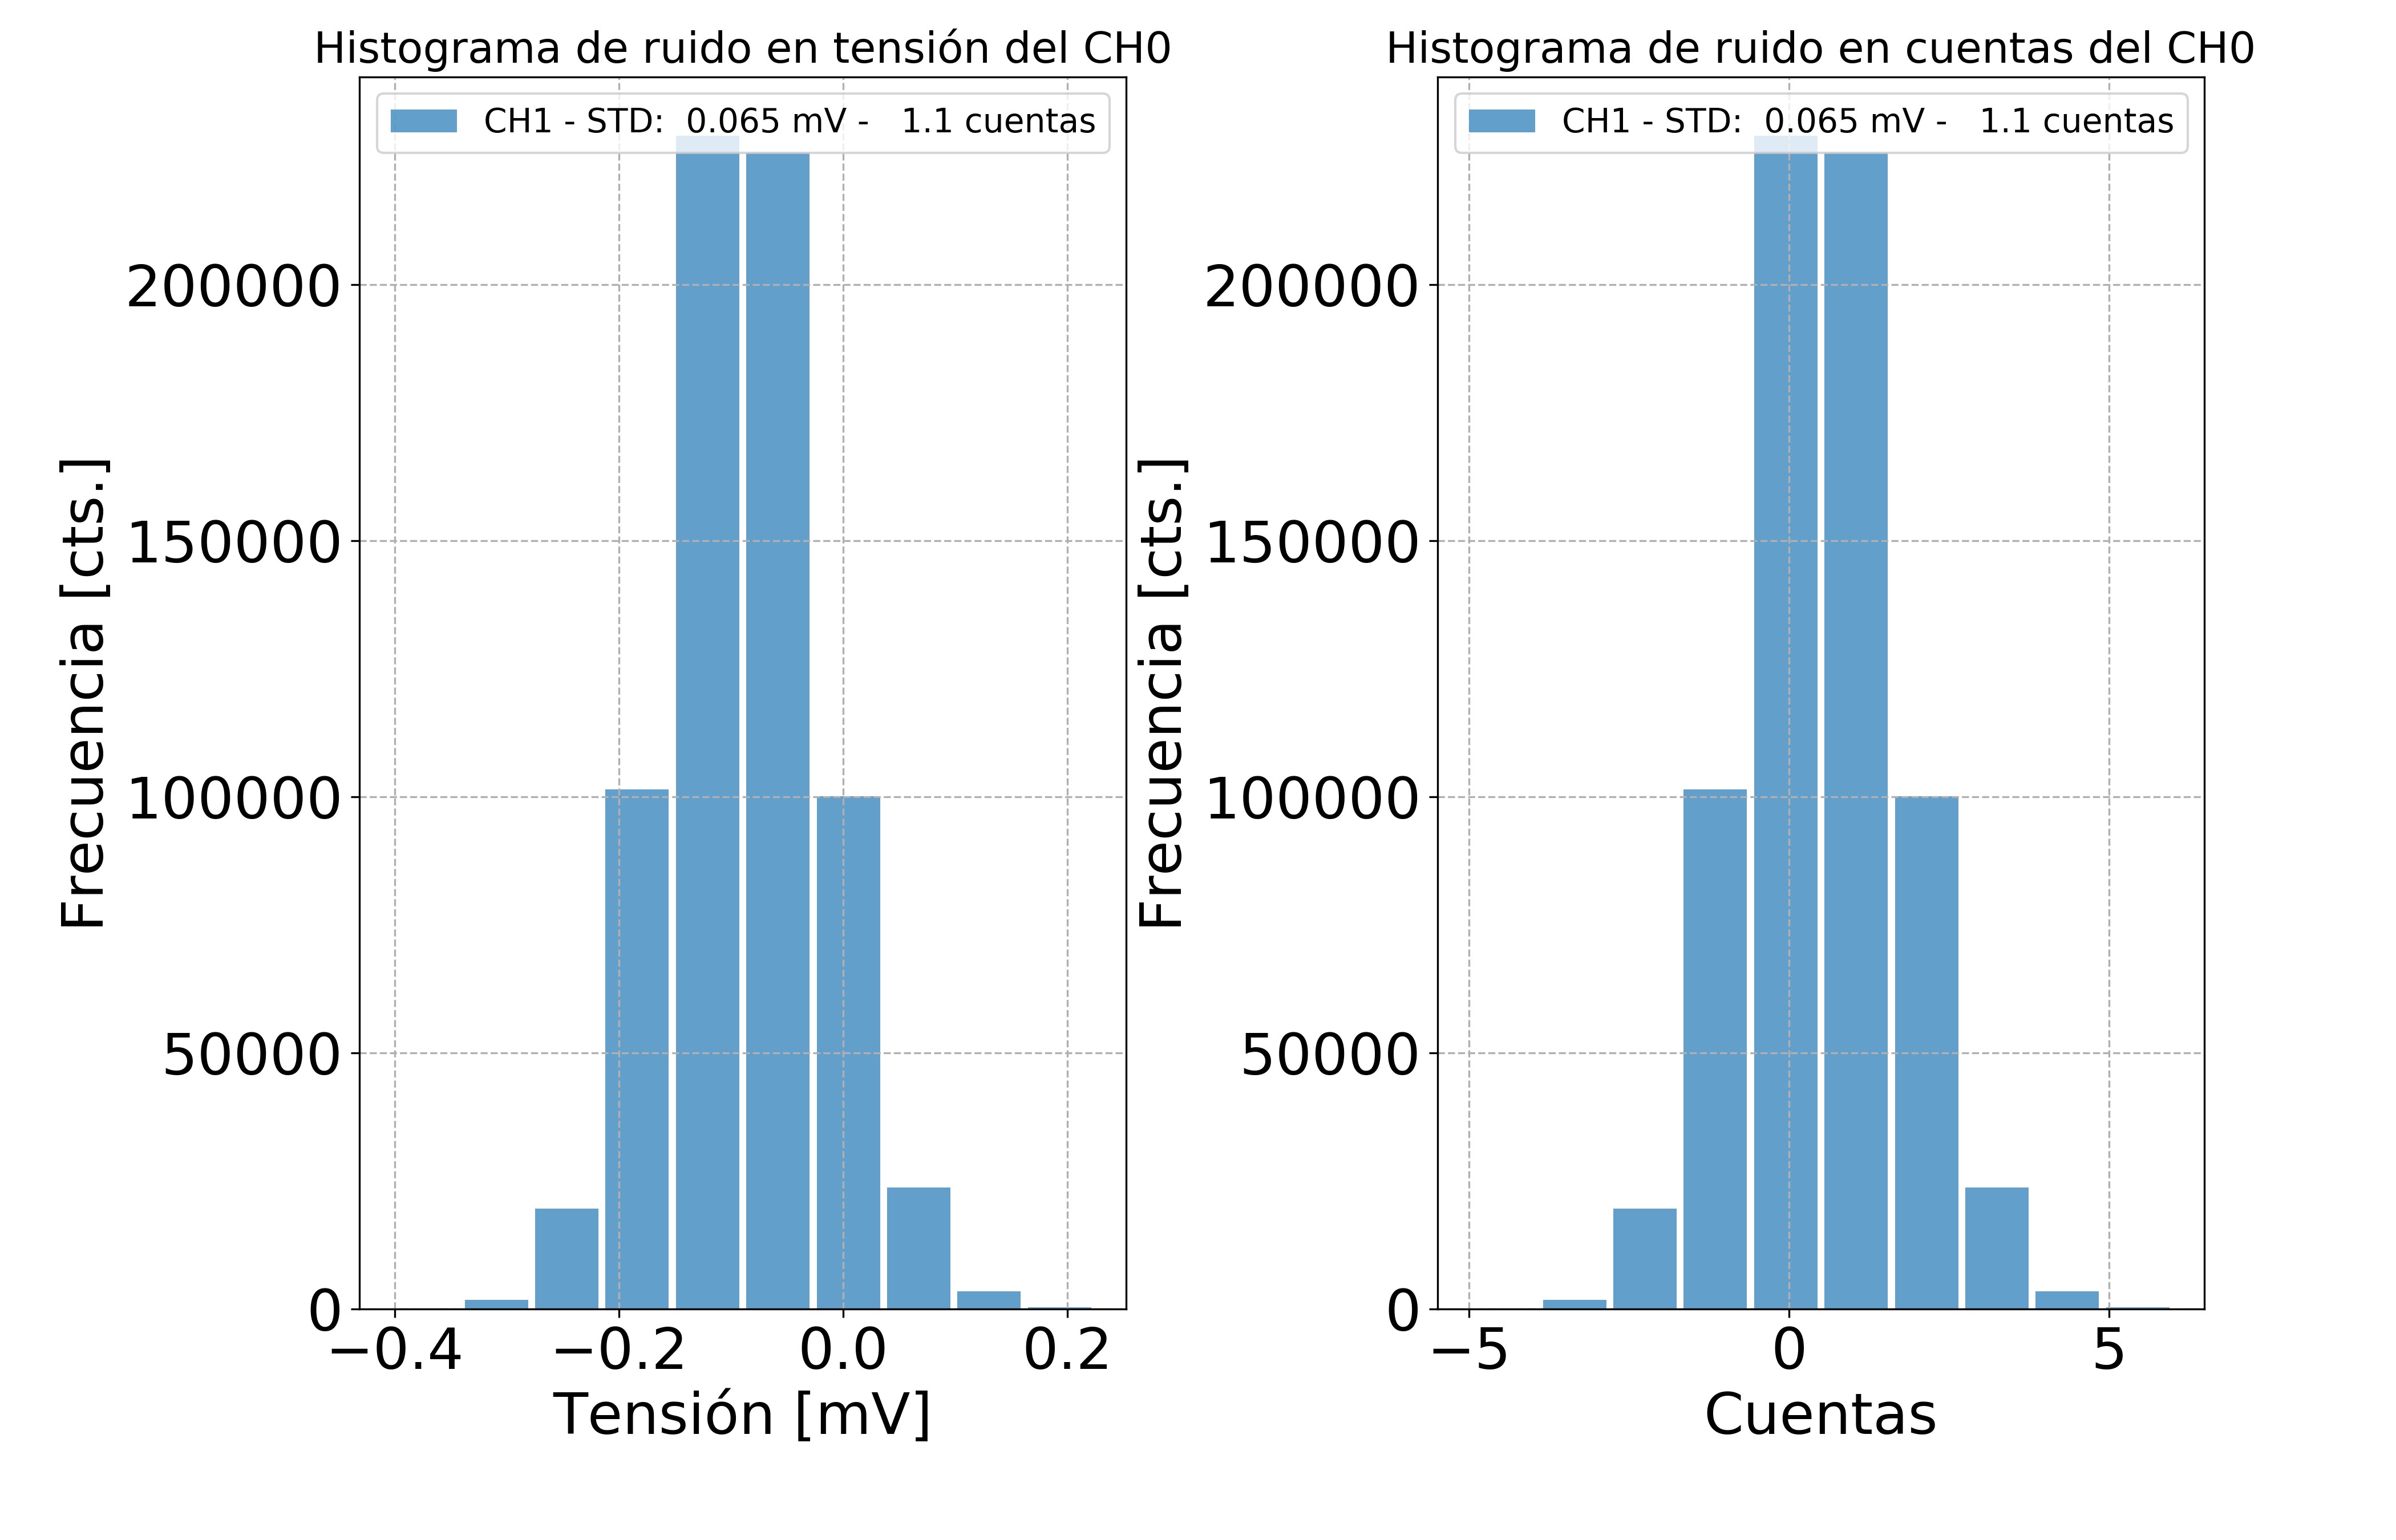
\includegraphics[scale=0.45]{ruido_cuentas_v_ch0.png}
\caption{Distribución de ruido en tensión y cuentas. La conversión a tensión se realizó utilizando la calibración del micrófono para un nivel de 50/100.\label{fig:ruidocuentas}}
\end{figure} 

Además nos propusimos determinar la dependencia del ruido con el nivel del micrófono. En la Figura \ref{fig:ruidomic}  se muestran los resultados y como era esperable se observa un aumento de los niveles de ruido en cuentas a medida que aumentamos la amplificación de la señal. Sin embargo se observa una disminución en tensión de dichos niveles de ruido, obtenido a partir de utilizar la calibración de la Tabla 1. Esto nos estaría indicando que la relación señal a ruido de la señal adquirida (SNR) debería mejorar a medida que aumentamos el nivel de micrófono (sin saturar la señal).

\begin{figure} [H]
\centering
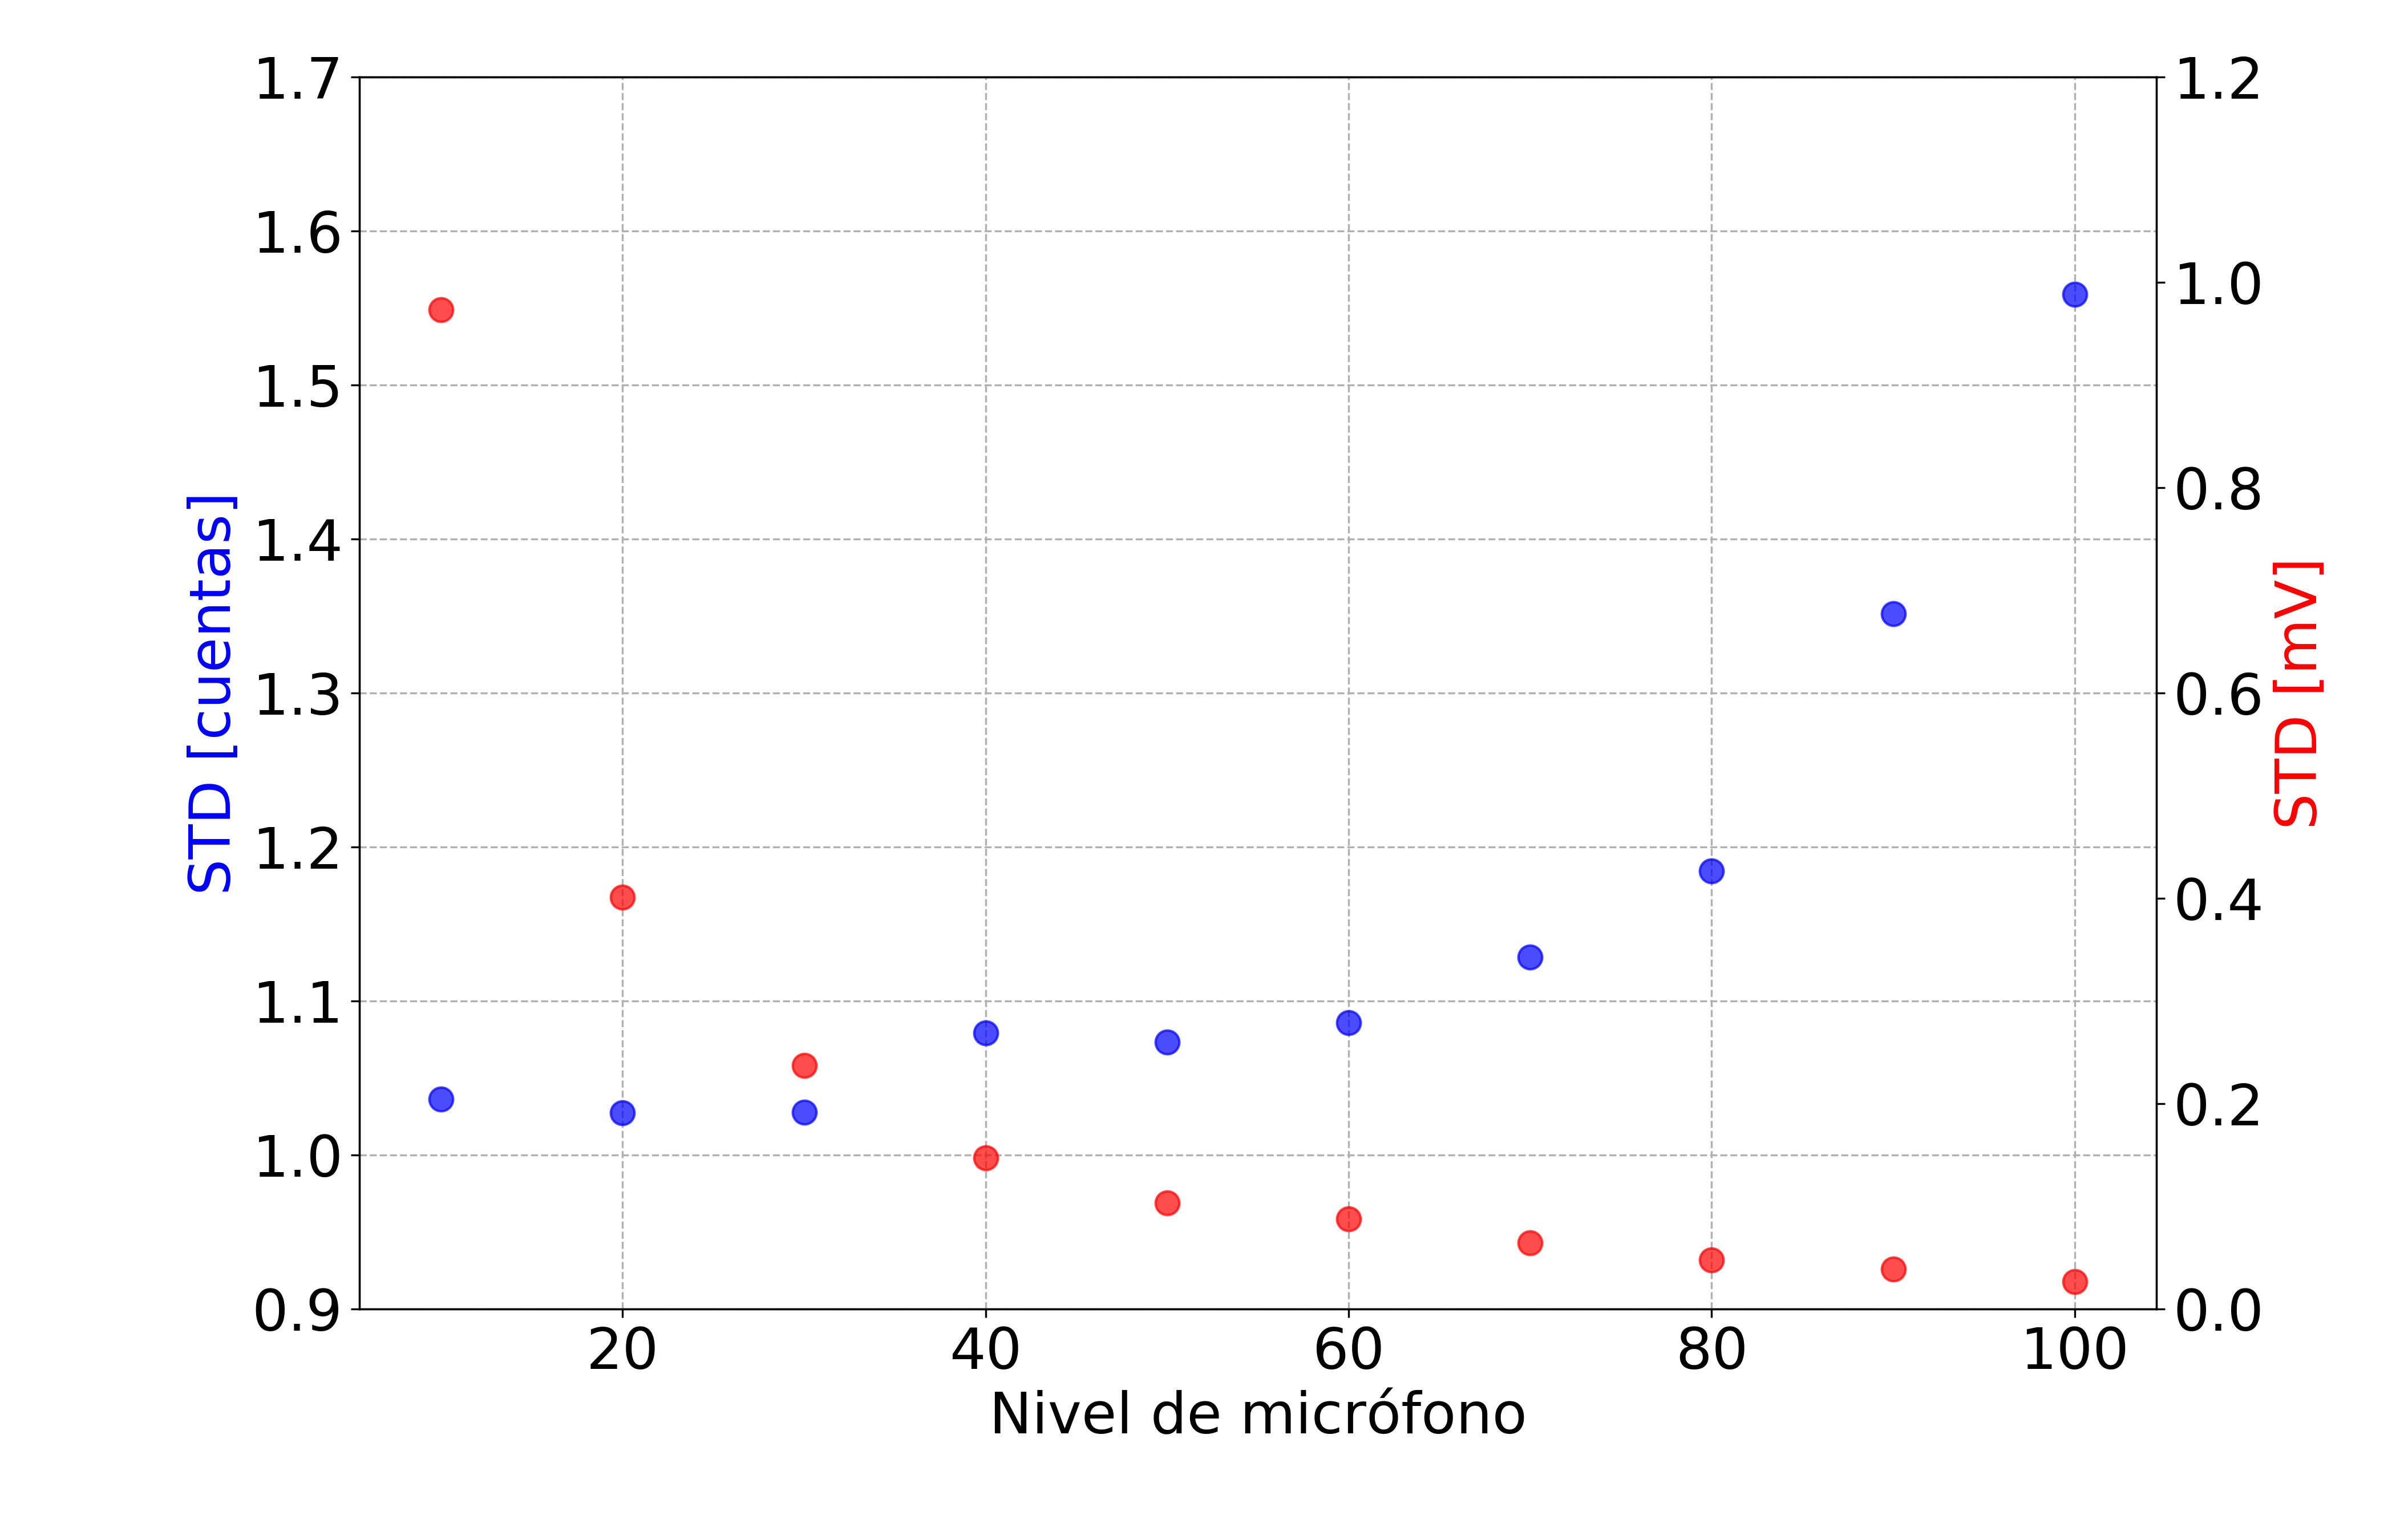
\includegraphics[scale=0.45]{ruido_nivel_microfono_ch0.png}
\caption{Desviación estándar del ruido (STD) en función del nivel de micrófono en cuentas (azul) y tensión (rojo). Si bien se observa un aumento del ruido en cuentas al aumentar el nivel de micrófono, el ruido en tensión baja. \label{fig:ruidomic}}
\end{figure} 

\subsection*{Relación señal ruido (SNR)}
Para medir la relación señal a ruido (SNR) enviamos una señal seno de 1023 Hz y de amplitud fija de 0.3 V, de manera de asegurarnos no saturar la entrada para cada nivel de micrófono. Una vez obtenida la señal realizamos la descomposición espectral con la transformada rápida de Fourier y pasamos las mediciones a unidades de densidad de potencia espectral (Figura \ref{fig:potencia_mic100}). Para medir la SNR en potencia hicimos la relación entre el pico ubicado en 1023 Hz y el nivel basal (el promedio de la potencia espectral en el rango 1050 a 1500 Hz). En la Figura \ref{fig:snr} graficamos los valores en función del nivel de micrófono, donde observamos una mejora de la relación señal a ruido (azul) a medida que aumentamos en nivel de micrófono debido a una disminución de los niveles de ruido (rojo). Esto era esperable teniendo en cuenta la disminución de la desviación estándar del ruido a medida que aumentamos el nivel de micrófono que se observó al medir 0 V ( Figura \label{fig:ruidomic}).

\begin{figure} [H]
\centering
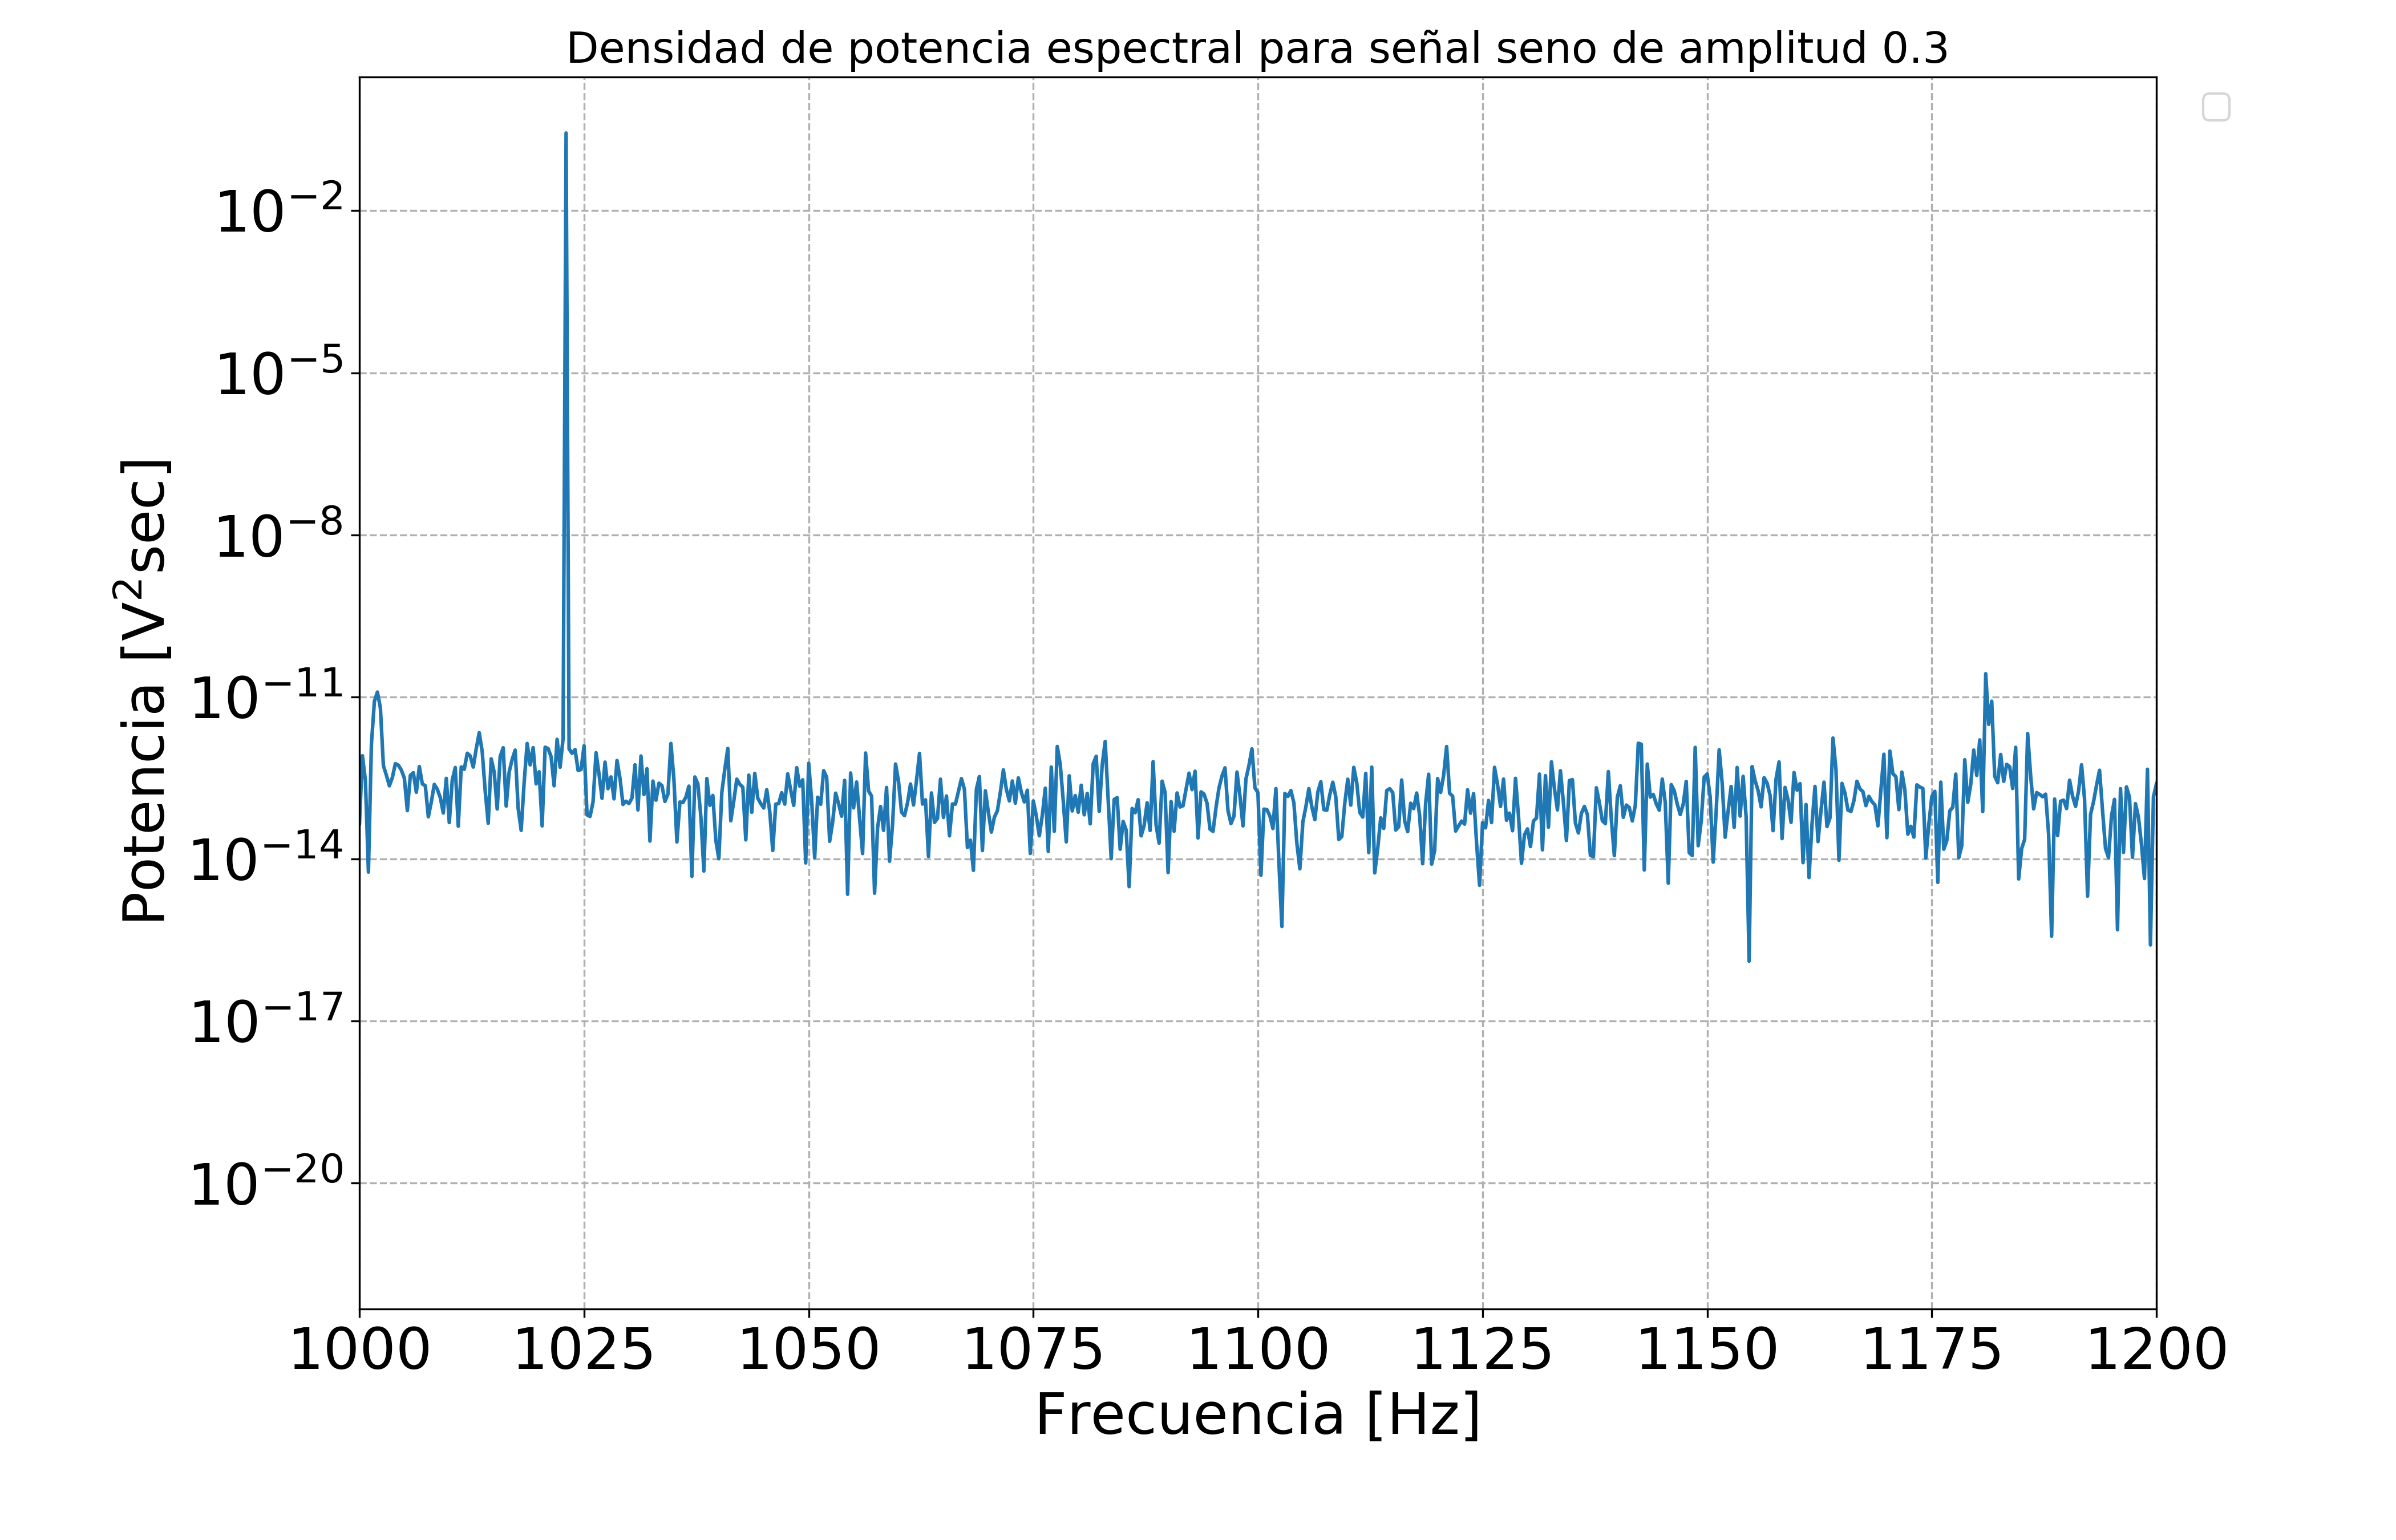
\includegraphics[scale=0.45]{potencia_mic100.png}
\caption{Espectro de potencias de señal sinusoidal de 1023 Hz utilizada para la medición de la SNR. Esta se calcula como la relación entre el pico y el valor basal del espectro de potencias. \label{fig:potencia_mic100}}
\end{figure} 

\begin{figure} [H]
\centering
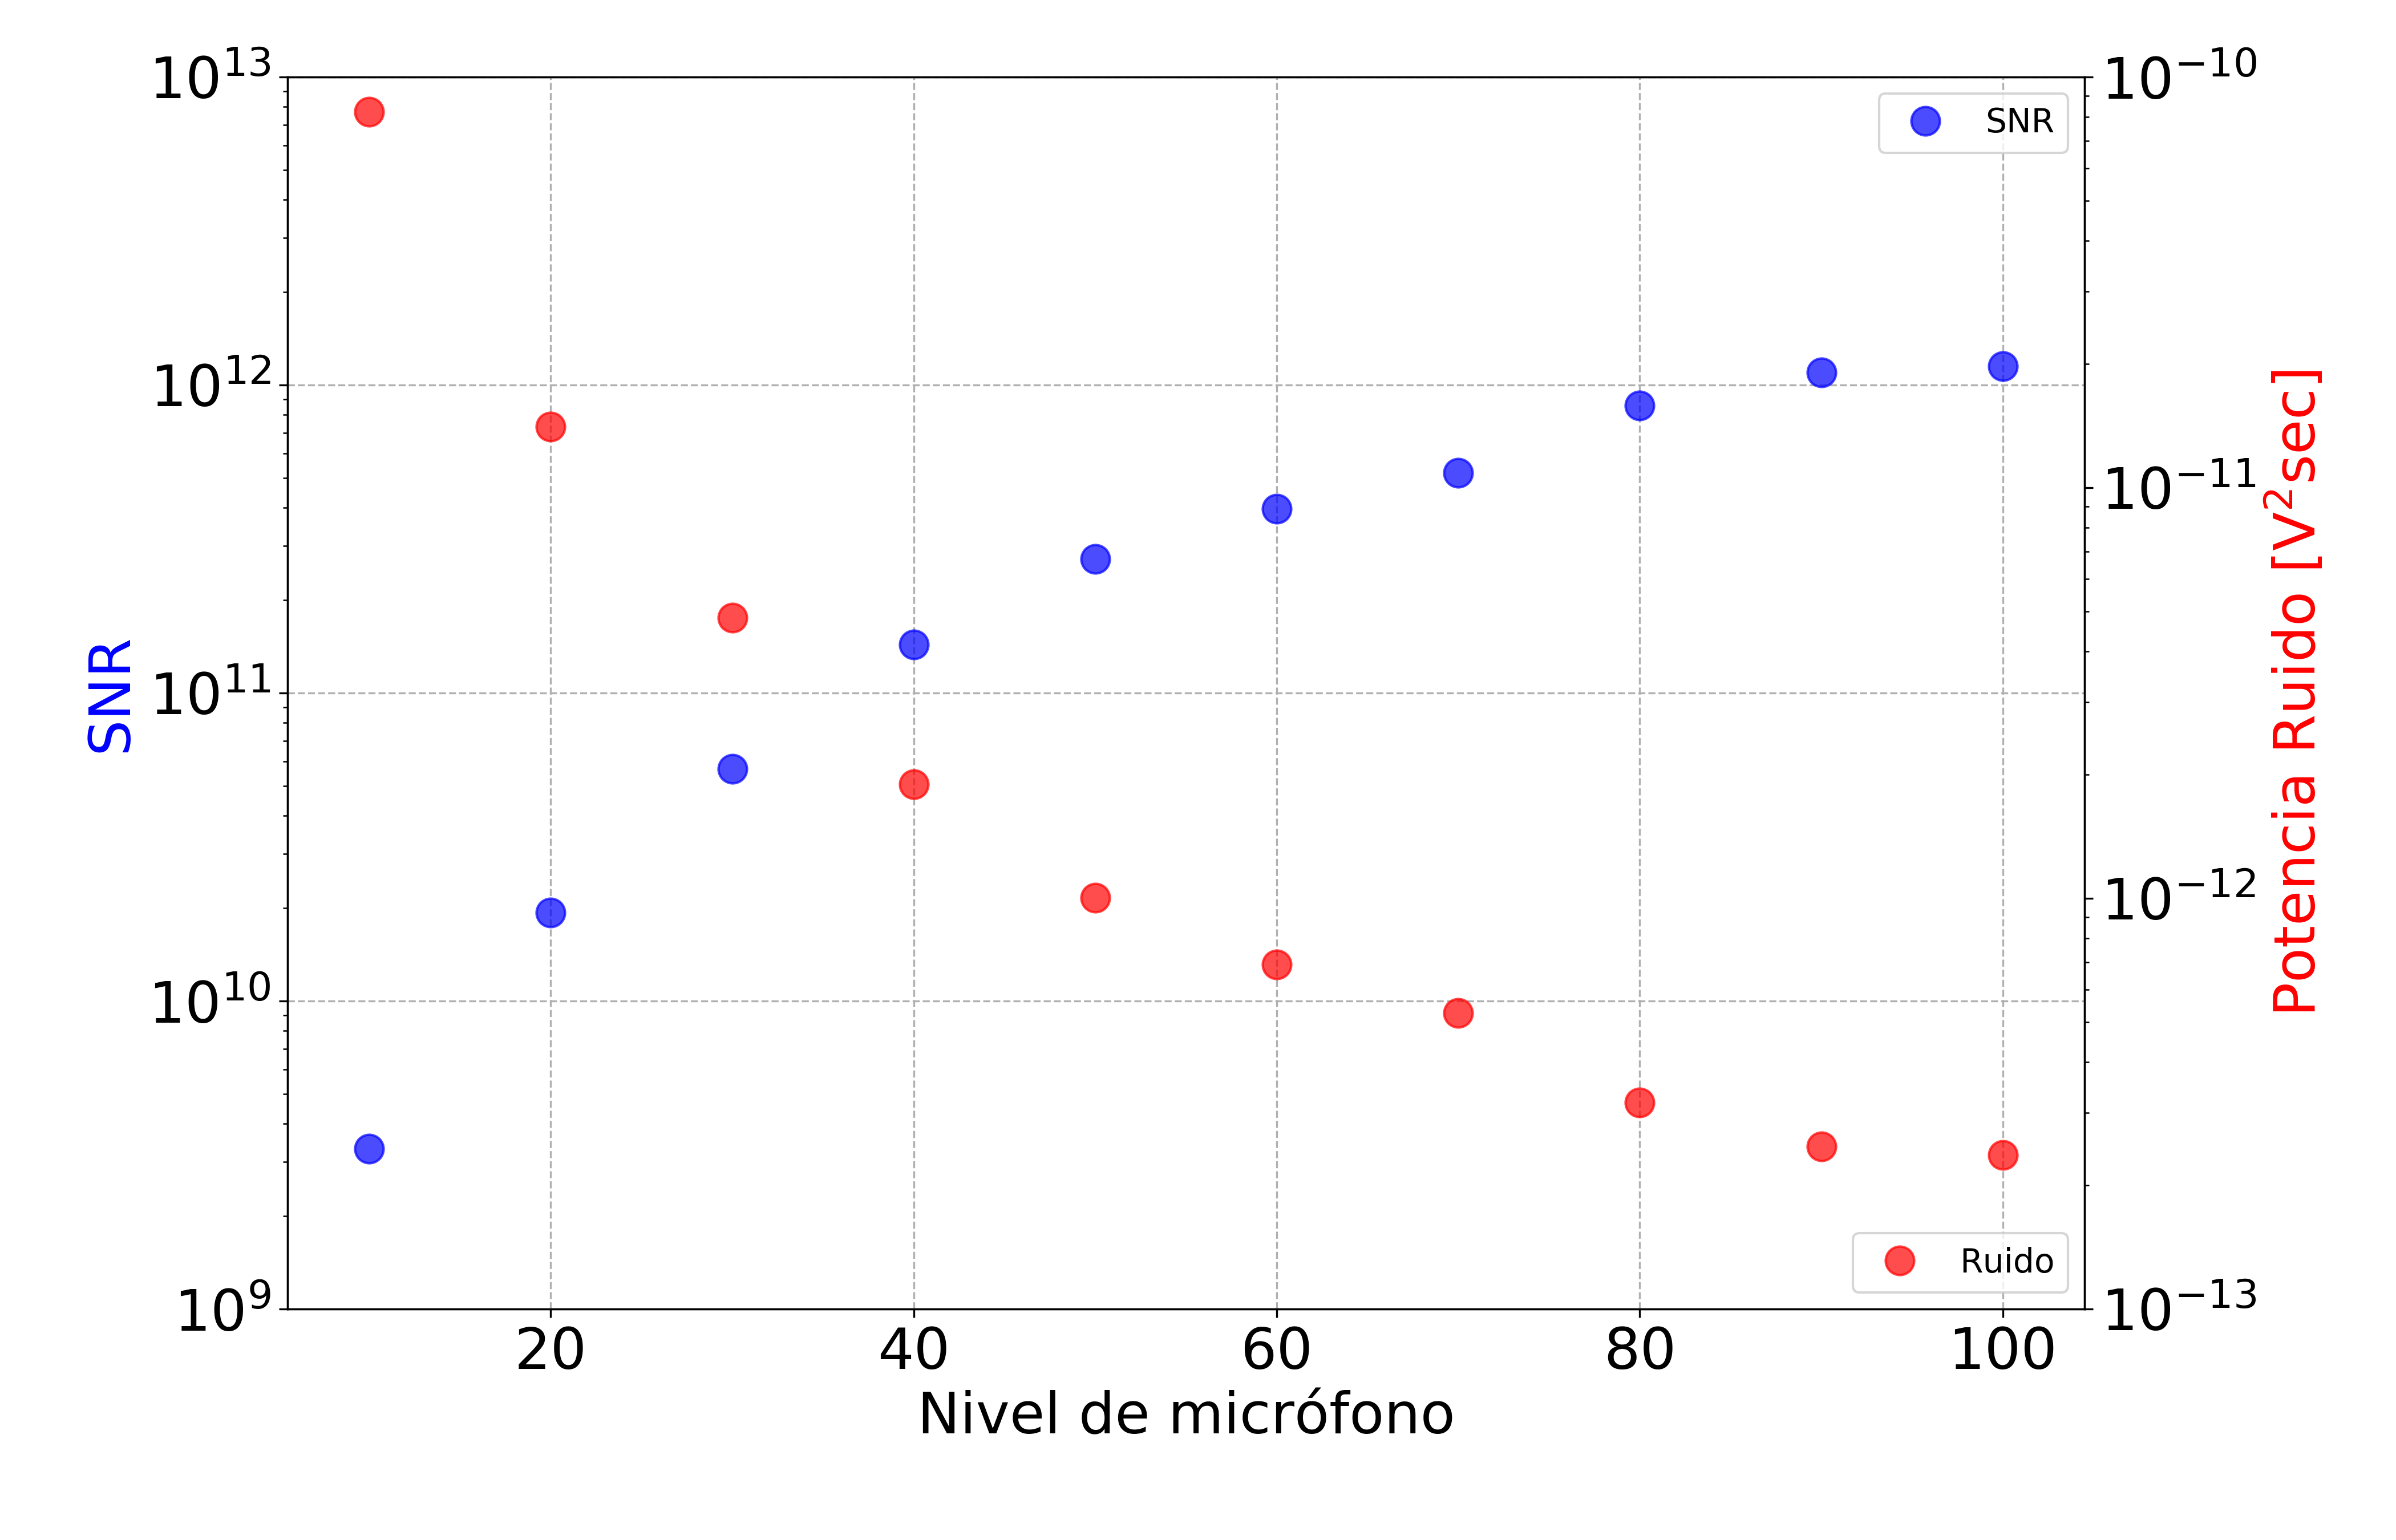
\includegraphics[scale=0.45]{snr_microfono_ch0.png}
\caption{SNR para el canal CH0 para distintos niveles de micrófono (azul) y promedio del valor basal del ruido entre 1050 Hz y 1500 Hz. Se observa un aumento del SNR a medida que aumentamos el nivel de micrófono debido a una diminución de los niveles de ruido. \label{fig:snr}}
\end{figure} 


%También nos propusimos estudiar el ruido en función de la frecuencia de sampleo. En la Figura \ref{fig:fft_ruido} mostramos el espectro del ruido para distintas frecuencias de sampleo. En el gráfico se observa que el ruido de baja frecuencia es de mayor amplitud que al de alta para todas las frecuencias de sampleo. Además se observa plano por partes, y en particular se nota un escalón en aproximadamente 20 kHz que coincide (como vimos anteriormente) con el ancho de banda del sistema emisor-receptor. Esta disminución en el ruido podría deberse entonces a que el ruido de temperatura (o de ancho de banda) a partir de esta frecuencia de corte no aporta al ruido total. A continuación en la Figura \ref{fig:std_frec_sampleo} mostramos como varia la desviación estándar del ruido a medida que cambiamos la frecuencia de sampleo. Como era esperable se observa un aumento del ruido a medida que aumentamos la frecuencia de sampleo %(y por lo tanto el ancho banda?? Esto no se). El aumento más lento para frecuencias de sampleo altas podría deberse a que efectivamente no estamos considerando ruido de ancho de banda (¿?????). 
%En el mismo gráfico mostramos la desviación estándar al aplicar de un filtro de media a los datos adquiridos a frecuencia de sampleo más alta. Si se aplica un filtro de media de N muestras le asignamos ese valor a la frecuencia FrecSsampleo/N. 
%
%\begin{figure} [H]
%\centering
%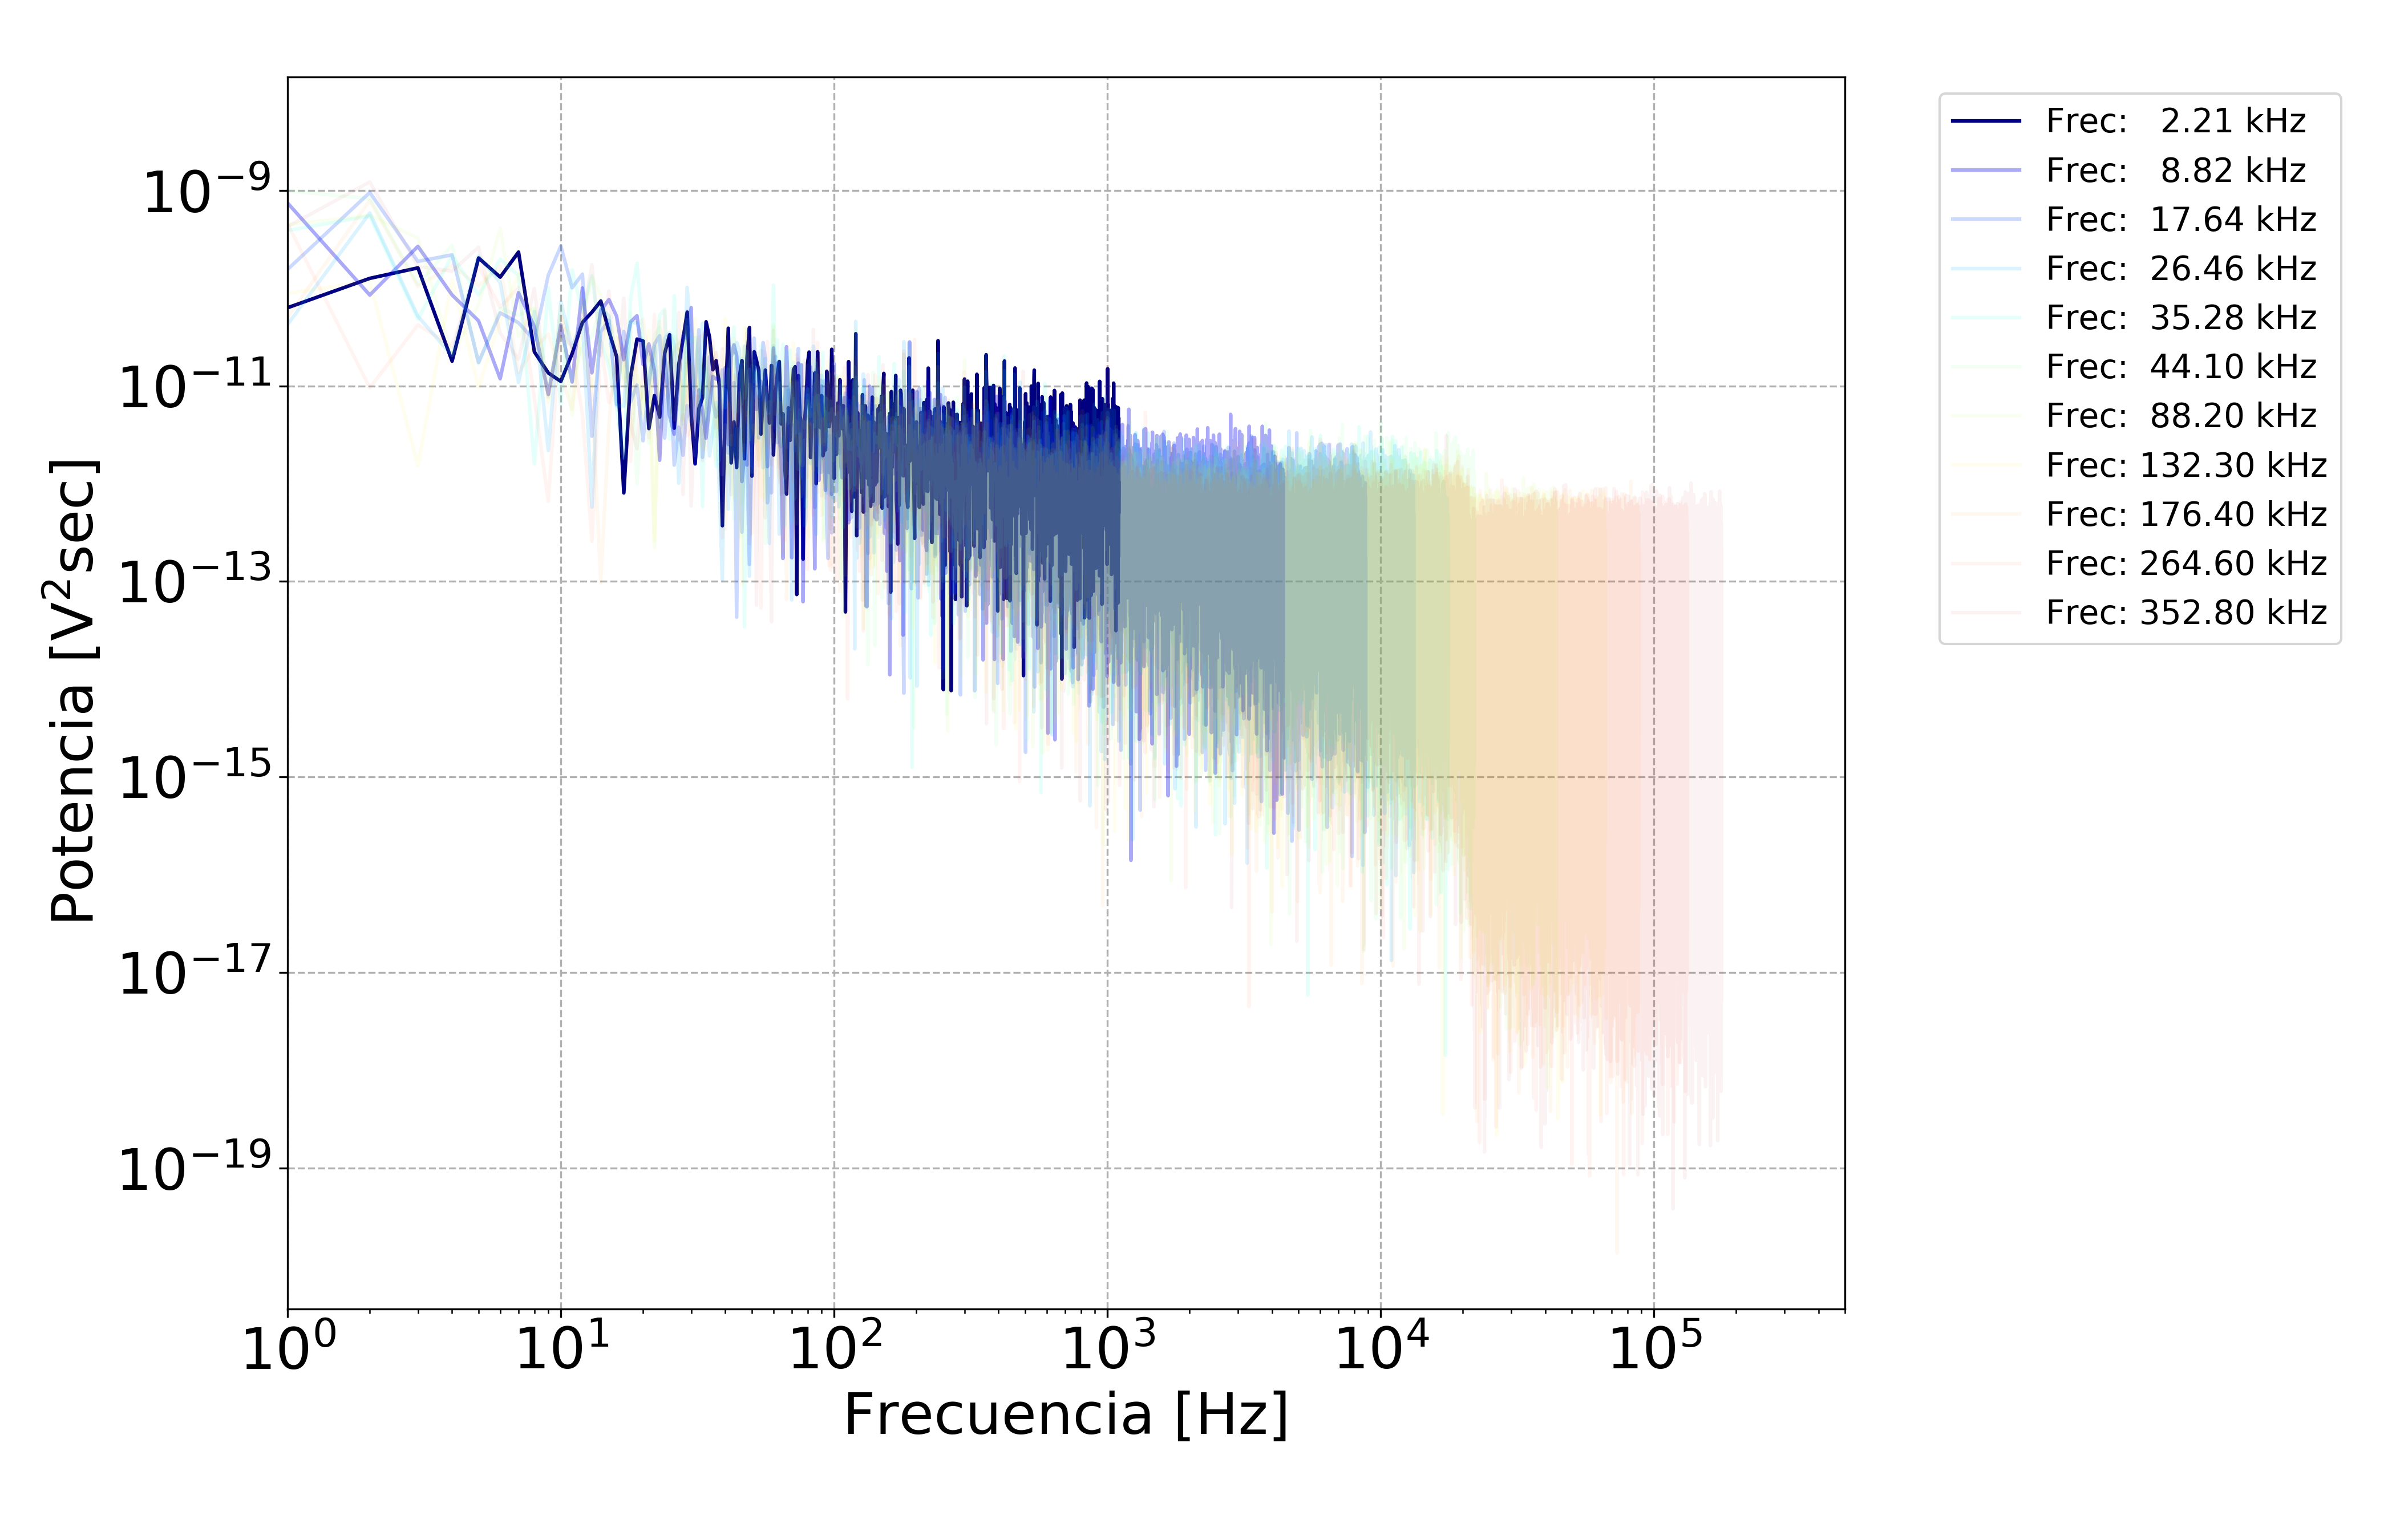
\includegraphics[scale=0.45]{fft_ruido.png}
%\caption{Espectro del ruido para distintas frecuencias de sampleo. Nivel de micrófono 70/100. \label{fig:fft_ruido}}
%\end{figure} 
%
%\begin{figure} [H]
%\centering
%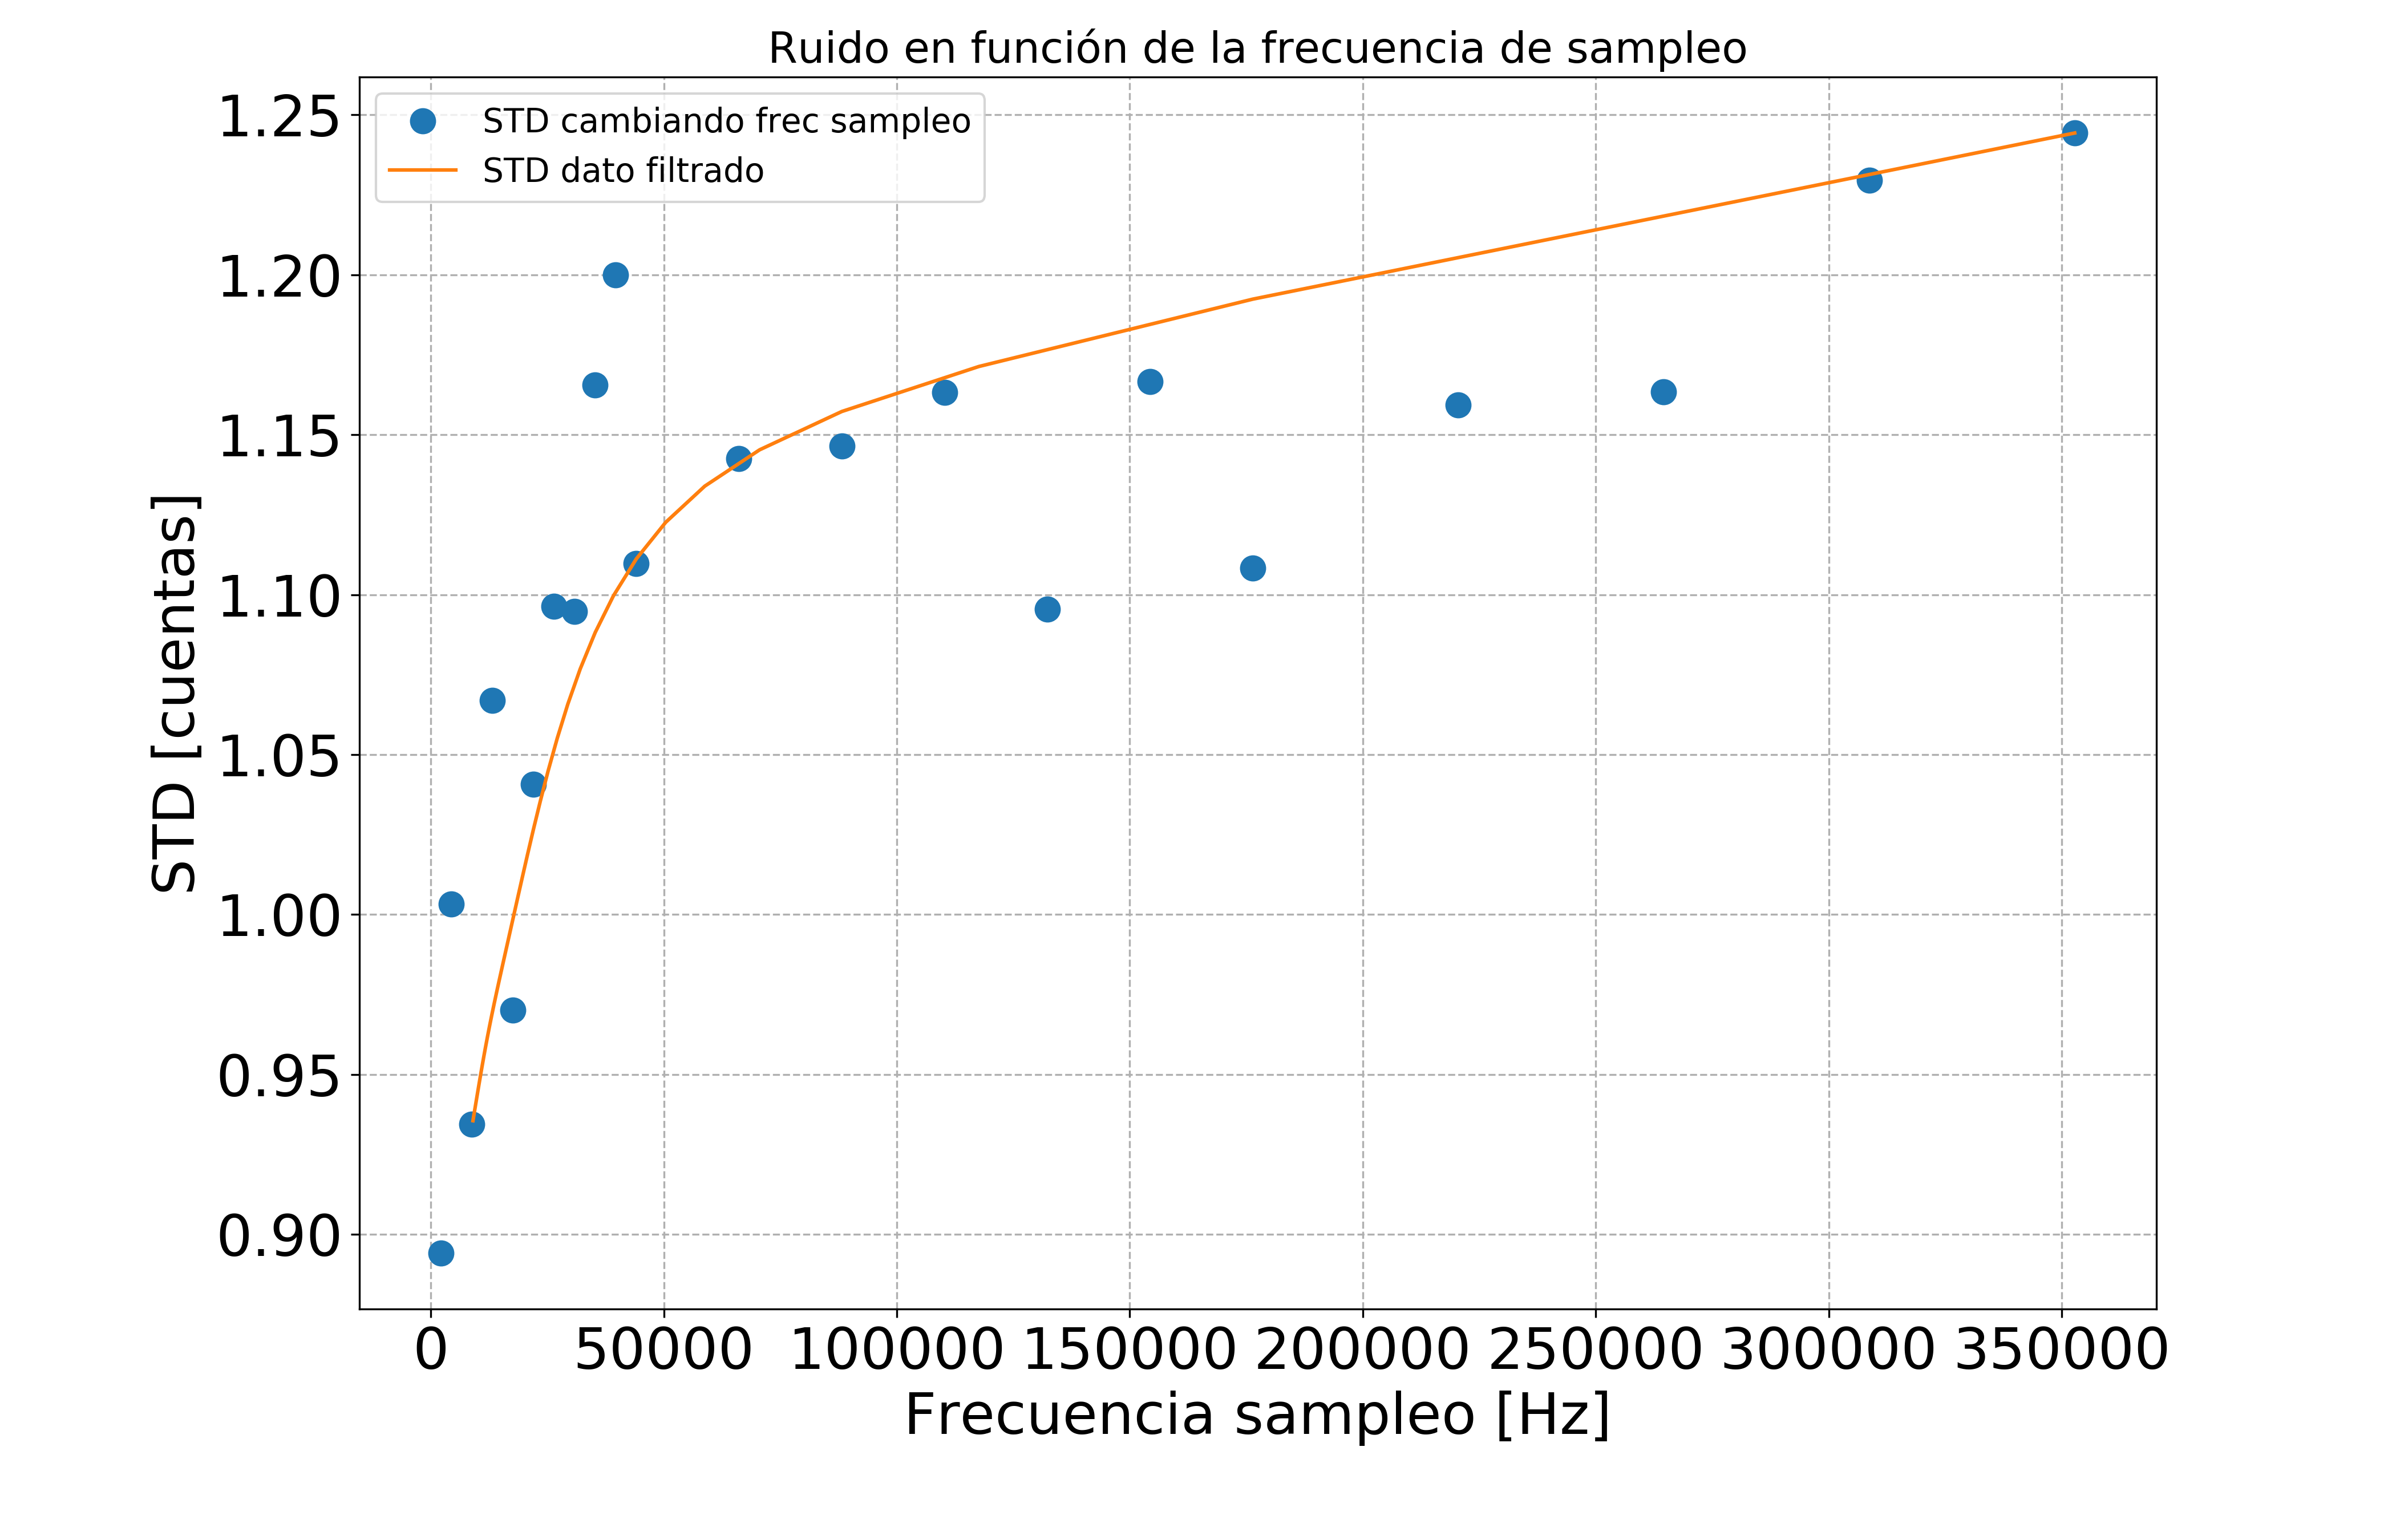
\includegraphics[scale=0.45]{std_frec_sampleo.png}
%\caption{Aumento del ruido con la frecuencia de sampleo. El cambio de tendencia luego de los 44 kHz podría indicar que a partir de ese valor no estamos considerando el ruido de ancho de banda, que domina a frecuencias menores. La curva naranja se obtiene al aplicar un filtro de media a los datos N muestras asignada a la frecuencia FrecSsampleo/N.\label{fig:std_frec_sampleo}}
%\end{figure} 


\subsection*{Crosstalk}
Por otro lado medimos crosstalk entre canales. Para ello enviamos una señal seno a una frecuencia de 1023 Hz en el canal CH0 y medimos un cero en el canal CH1, y luego medimos en los gráficos de densidad de potencia espectral las relación señal a ruido de ambos canales (Figura \ref{fig:crosstalk_mic100} ). En este caso obtenemos un valor de SNR de orden 12 en el canal CH0 y de orden 2 en el canal CH1,  y por lo tanto a una relación de SNR de orden 10 entre canales (equivalente a un orden 5 en amplitud).  Es decir que si medimos señales del orden de 1 V en el canal CH0 es esperable un nivel de señal de 10 mV en el canal CH1.

\begin{figure} [H]
\centering
\includegraphics[scale=0.45]{crosstalk_mic100.png}
\caption{Crosstalk entre canales CH0 y CH1. \label{fig:crosstalk_mic100}}
\end{figure} 

\subsection*{Resolución en frecuencias}
A continuación nos propusimos medir la exactitud y la resolución en frecuencias de la placa de audio. Para la exactitud consideramos la diferencia en la frecuencia entre la señal enviada y la adquirida; mientras que para la resolución enviamos una señal compuesta por dos frecuencias cercanas y vemos si es posible distinguirlas en el espectro de frecuencias medido. En este caso medimos ambos parámetros con un sólo experimento que consiste en enviar una señal suma de dos senos a frecuencias 1023.020 y 1023.022. La medición se realizó a una frecuencia de sampleo de 44100 Hz y se eligió una duración de la señal de 1000 segundos para asegurarnos tener un espaciado en frecuencias en el espectro de 1 mHz (recordar que el sampleo en frecuencias en el espectro es la inversa de la duración de la señal). En principio podríamos utilizar señales de mayor duración para mejorar el sampleo en frecuencias pero esto no fue posible por limitaciones en el buffer de salida de la placa de audio. En la Figura  \ref{fig:resolucion_frecuencia} observamos el espectro de frecuencias de la señal enviada y adquirida, donde verificamos que las frecuencias medidas son las mismas que las enviadas y además observamos que es posible distinguir frecuencias cercanas, en nuestro caso distanciadas por 2 mHz. Por lo tanto podemos asegurar que tanto la exactitud como la resolución en frecuencias es por lo menos 1 mHz equivalente a 1 ppm (tener en cuenta que la relación entre la resolución y la frecuencia enviada es de $10^{-6}$)


\begin{figure} [H]
\centering
\includegraphics[scale=0.45]{resolucion_frecuencia.png}
\caption{Espectro de frecuencias de señal enviada y adquirida de una suma de senos a 1023.020 Hz y 1023.022 Hz. Se verifica que la exactitud y la resolución en frecuencias es mejor a 1 mHz.\label{fig:resolucion_frecuencia}}
\end{figure} 


\subsection*{Hoja de datos}
A modo de conclusión, pudimos confeccionar la siguiente tabla que resume las características principales del sistema:
\begin {table}[H]
\begin {center}
 \begin{tabular} {|l|c|}
        \hline
        Ancho de banda & 20kHz \\
        \hline
        Rango de frecuencia & 14 Hz - 20 kHz\\
        \hline
        Máxima tensión de salida  & 3.2 V\\
        \hline
        Máxima tensión de entrada  & 2.10 V\\
        \hline
        Resolución de la entrada  & 16 bits\\
        \hline
	\multicolumn{2}{|l|}{Ruido entrada (@ fs: 352800 Hz)} \tabularnewline
        \hline
        0 V (@ mic 10/100) & Std: 1.036 cts (973 $\mu V$)  - 8.5 $ \frac{\mu V}{\sqrt{Hz}}$ \\
        0 V (@ mic 100/100) & Std: 1.558 cts (26 $\mu V$) - 0.38 $ \frac{\mu V}{\sqrt{Hz}}$ \\
        \hline
         seno 1023 Hz, 0.3 V amp (@ mic 10/100) & 9.1 $ \frac{\mu V}{\sqrt{Hz}}$\\
	seno 1023 Hz, 0.3 V amp (@ mic 100/100) & 0.49 $ \frac{\mu V}{\sqrt{Hz}}$\\
        \hline
	\multicolumn{2}{|l|}{SNR potencia (@ fs: 352800 Hz)} \tabularnewline
        \hline
         seno 1023 Hz, 0.3 V amp (@ mic 10/100) & 95 db \\
	seno 1023 Hz, 0.3 V amp (@ mic 100/100) & 120 db \\
	\hline
	\multicolumn{2}{|l|}{Crosstalk potencia (CH0 a CH1) (@ fs: 352800 Hz)} \tabularnewline
	\hline
        seno 1023 Hz, 0.3 V amp (@ mic 10/100) & 91 db \\
	seno 1023 Hz, 0.3 V amp (@ mic 100/100) & 97 db \\
        \hline
\multicolumn{2}{|l|}{Frecuencia (@ fs: 44100 Hz) } \tabularnewline
        \hline
	Exactitud (@ seno 1023 Hz, 0.5 V Amp, 1000 s)  & 1 mHz (1 ppm @ 1000 Hz) \\
	Resolución (@ seno 1023 Hz, 0.5 V Amp, 1000 s) & 1 mHz (1 ppm @ 1000 Hz) \\
        % \hline
        % ADSDASD & ADASDAD\\
        \hline
 \end{tabular}
 \caption{Tabla de especificaciones del sistema emisor -receptor de la placa de sonido utilizada. Todos las mediciones fueron hechas a \SI{20}{\celsius} - \SI{25}{\celsius}}
 \label{table1}
 \end{center}
\end{table}

\section*{Caracterización de componentes}

\subsection*{Diodo}
\subsubsection*{Curva I-V}
Con el sistema caracterizado se midió la curva I-V del diodo según el esquema de la Figura \ref{fig:esquemadiodo}. Para ello enviamos una señal sinusoidal de amplitud mayor a la caída típica del diodo a fin de asegurarnos de polarizar el diodo. La resistencia se utiliza para limitar la corriente y se decide utilizar una de valor de 82 Ohms obteniendo un valor máximo de corriente de 10 mA. Con valores de resistencia menores se obtienen mayores valores de corriente, pero evitamos utilizar resistencias menores para no forzar el emisor. Con una resistencia de 10 Ohms se observa una caída en la tensión entre las terminales de salida, señal que le estamos pidiendo más corriente de la que está preparada.

\begin{figure} [H]
\centering
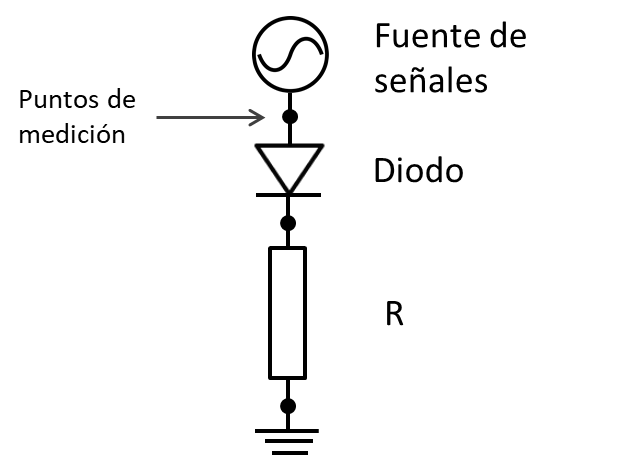
\includegraphics[scale=0.75]{esquema.png}
\caption{Esquema del circuito utilizado para la medición de la curva I-V del diodo \label{fig:esquemadiodo}}
\end{figure} 

En la Figura \ref{fig:caida_diodo_res_1N4007_82_20C_500hz_sin_corregir_offset_ajuste} se observa la caída de tensión total en el diodo y resistencia y la caída de tensión en la resistencia. La caída de tensión en la resistencia es cero a menos que el diodo se polarice con una tensión de umbral de aproximadamente 0.6 V. Como se puede observar en el gráfico a medida que transcurre la medición la tensión de la resistencia tiene un offset negativo que se estabiliza en -0.2 V. Esto es debido a que la respuesta a baja frecuencia del receptor está limitada y por lo tanto al perder la componente continua la señal sufre un corrimiento en tensión. En el gráfico se muestra el ajuste del decaimiento obteniendo un tiempo característico de 0.034 s. Notar que la caída total no sufre ningún corrimiento en tensión debido a que la señal no tiene componente de baja frecuencia. 
En la Figura \ref{fig:caida_diodo_res_1N4007_82_20C_500hz_fft} se muestra cómo al corregir la caída de tensión con un offset, se le está agregando una componente de baja frecuencia que el receptor recorta. En la Figura \ref{fig:caida_diodo_res_1N4007_82_20C_500hz} se muestra el detalle de la caída de tensión total, la caída en la resistencia corregida y la caída de tensión en el diodo como diferencia de las dos primeras.

\begin{figure} [H]
\centering
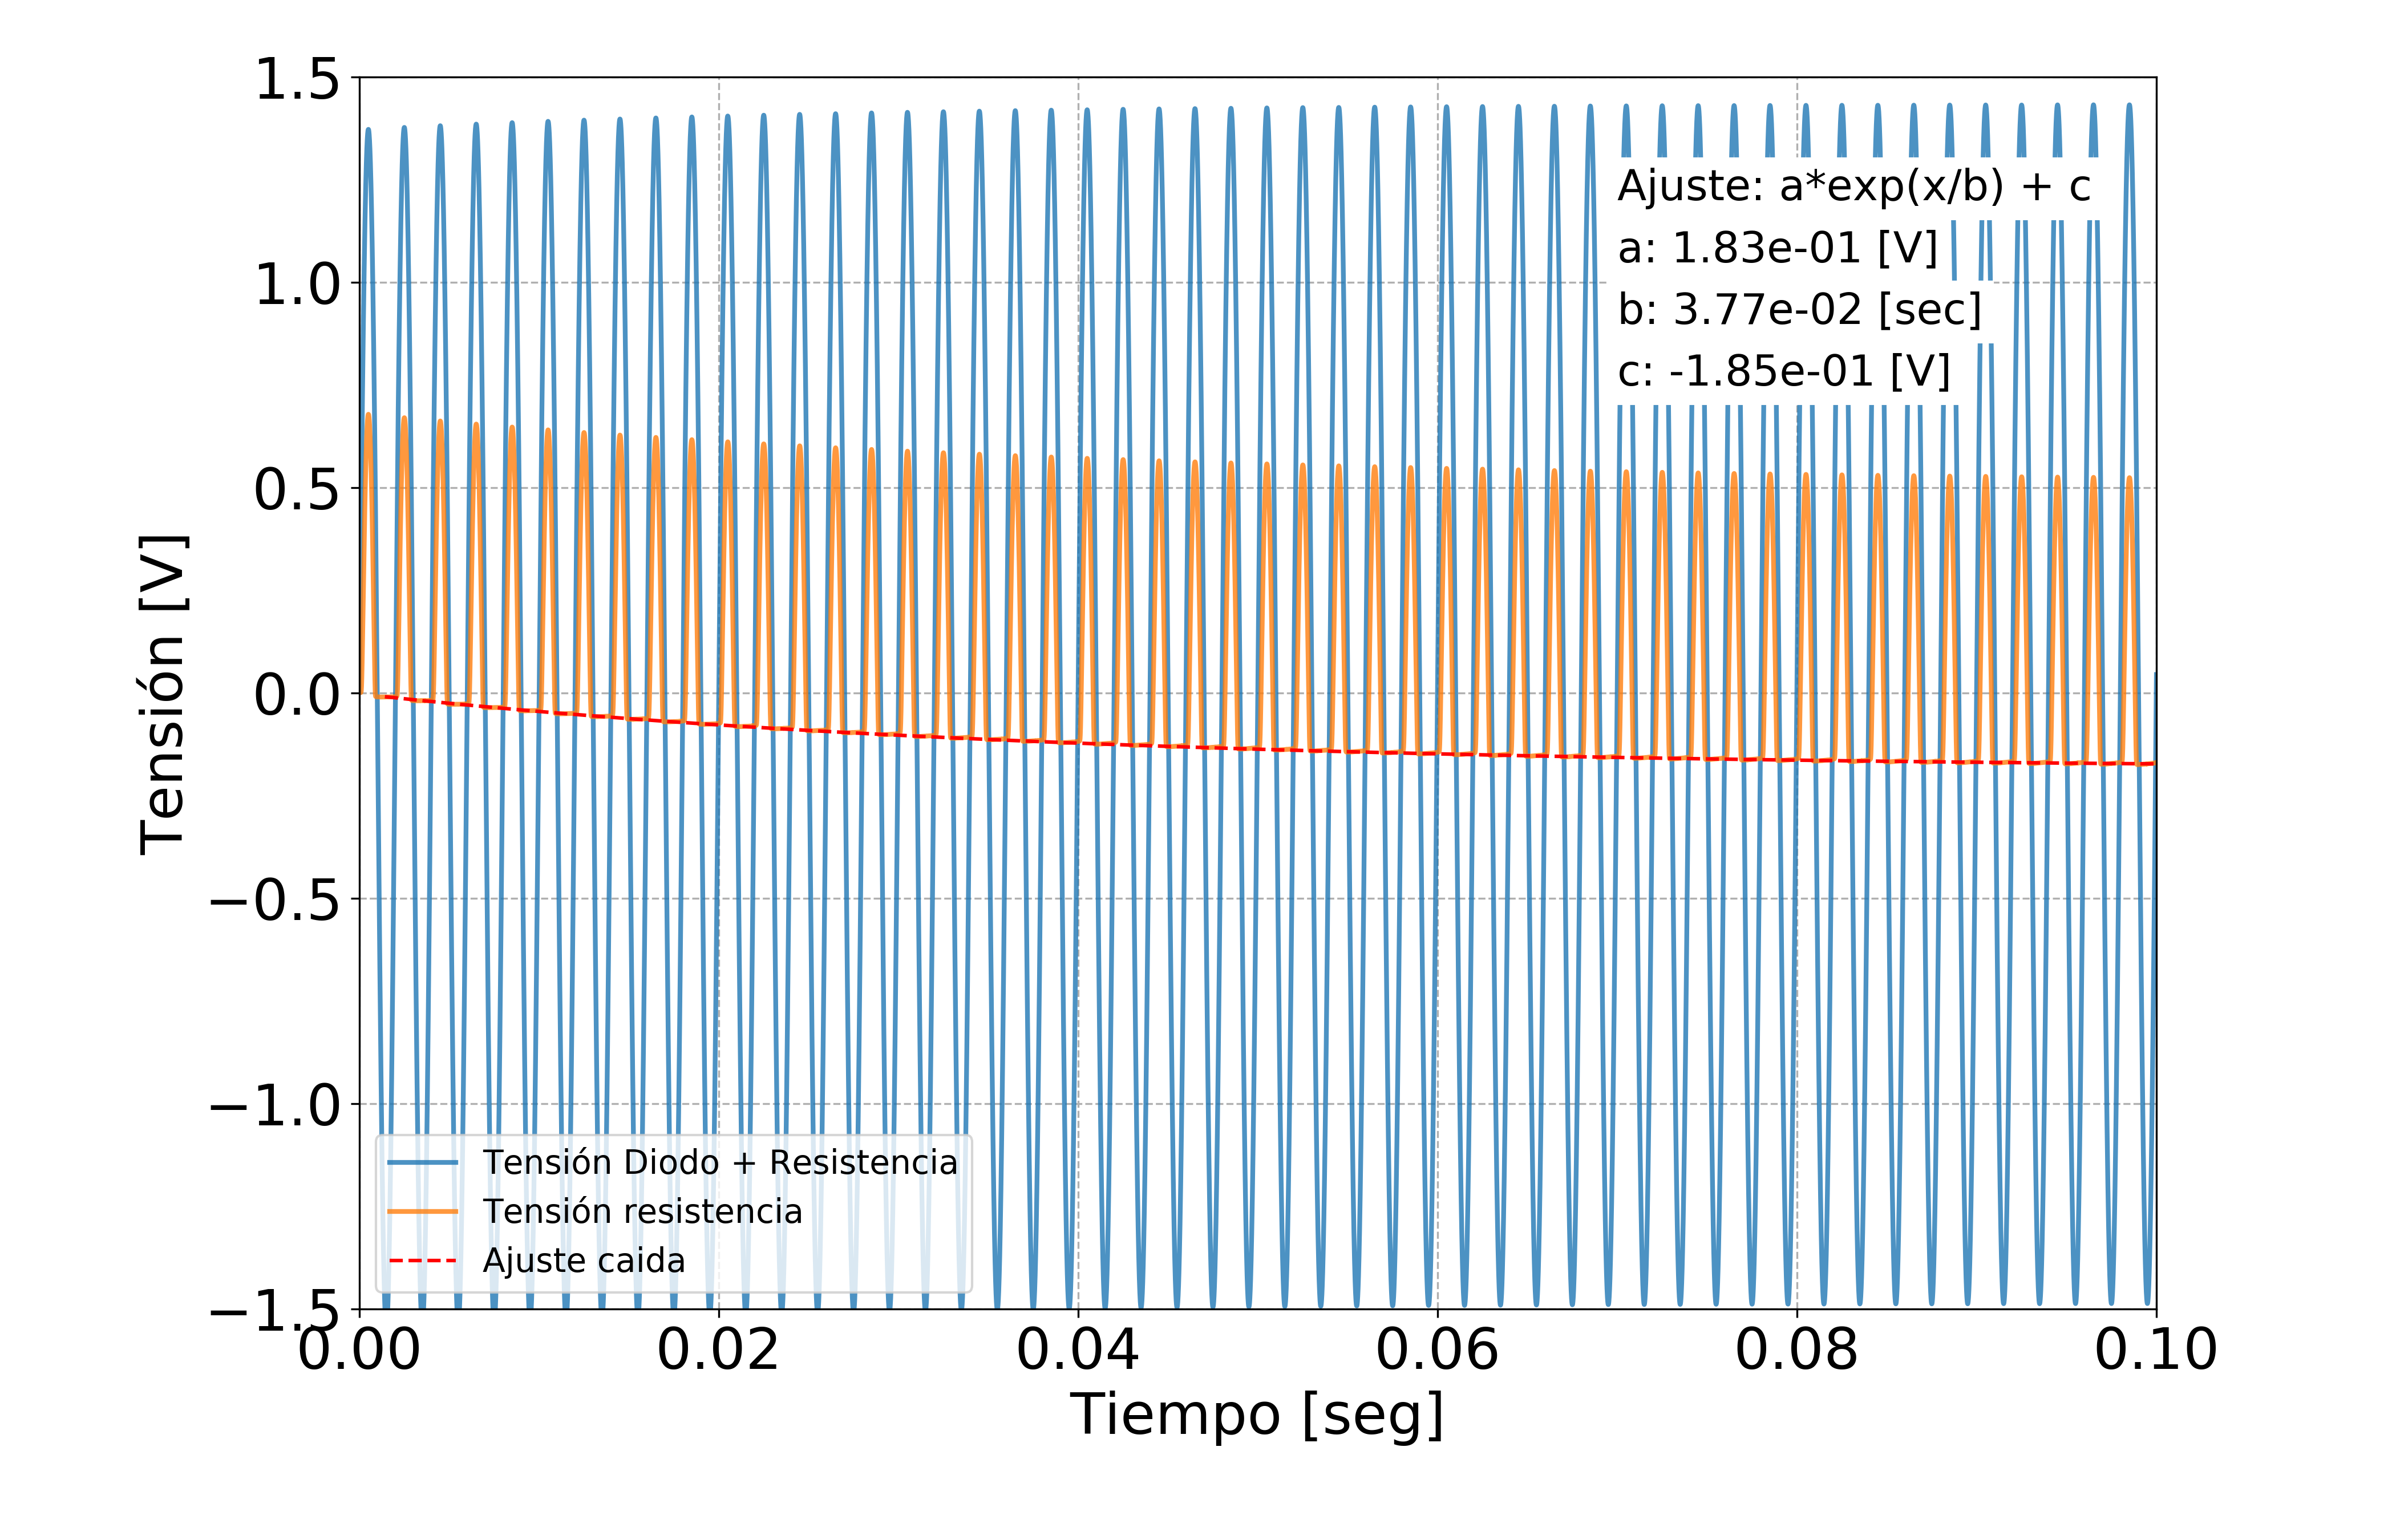
\includegraphics[scale=0.45]{caida_diodo_res_1N4007_82_20C_500hz_sin_corregir_offset_ajuste.png}
\caption{Caída de tensión total y sobre la resistencia al iniciar la medición. La caída que se observa a medida que transcurre la medición es debido a la limitación a baja frecuencia de la entrada. \label{fig:caida_diodo_res_1N4007_82_20C_500hz_sin_corregir_offset_ajuste}}
\end{figure} 

\begin{figure} [H]
\centering
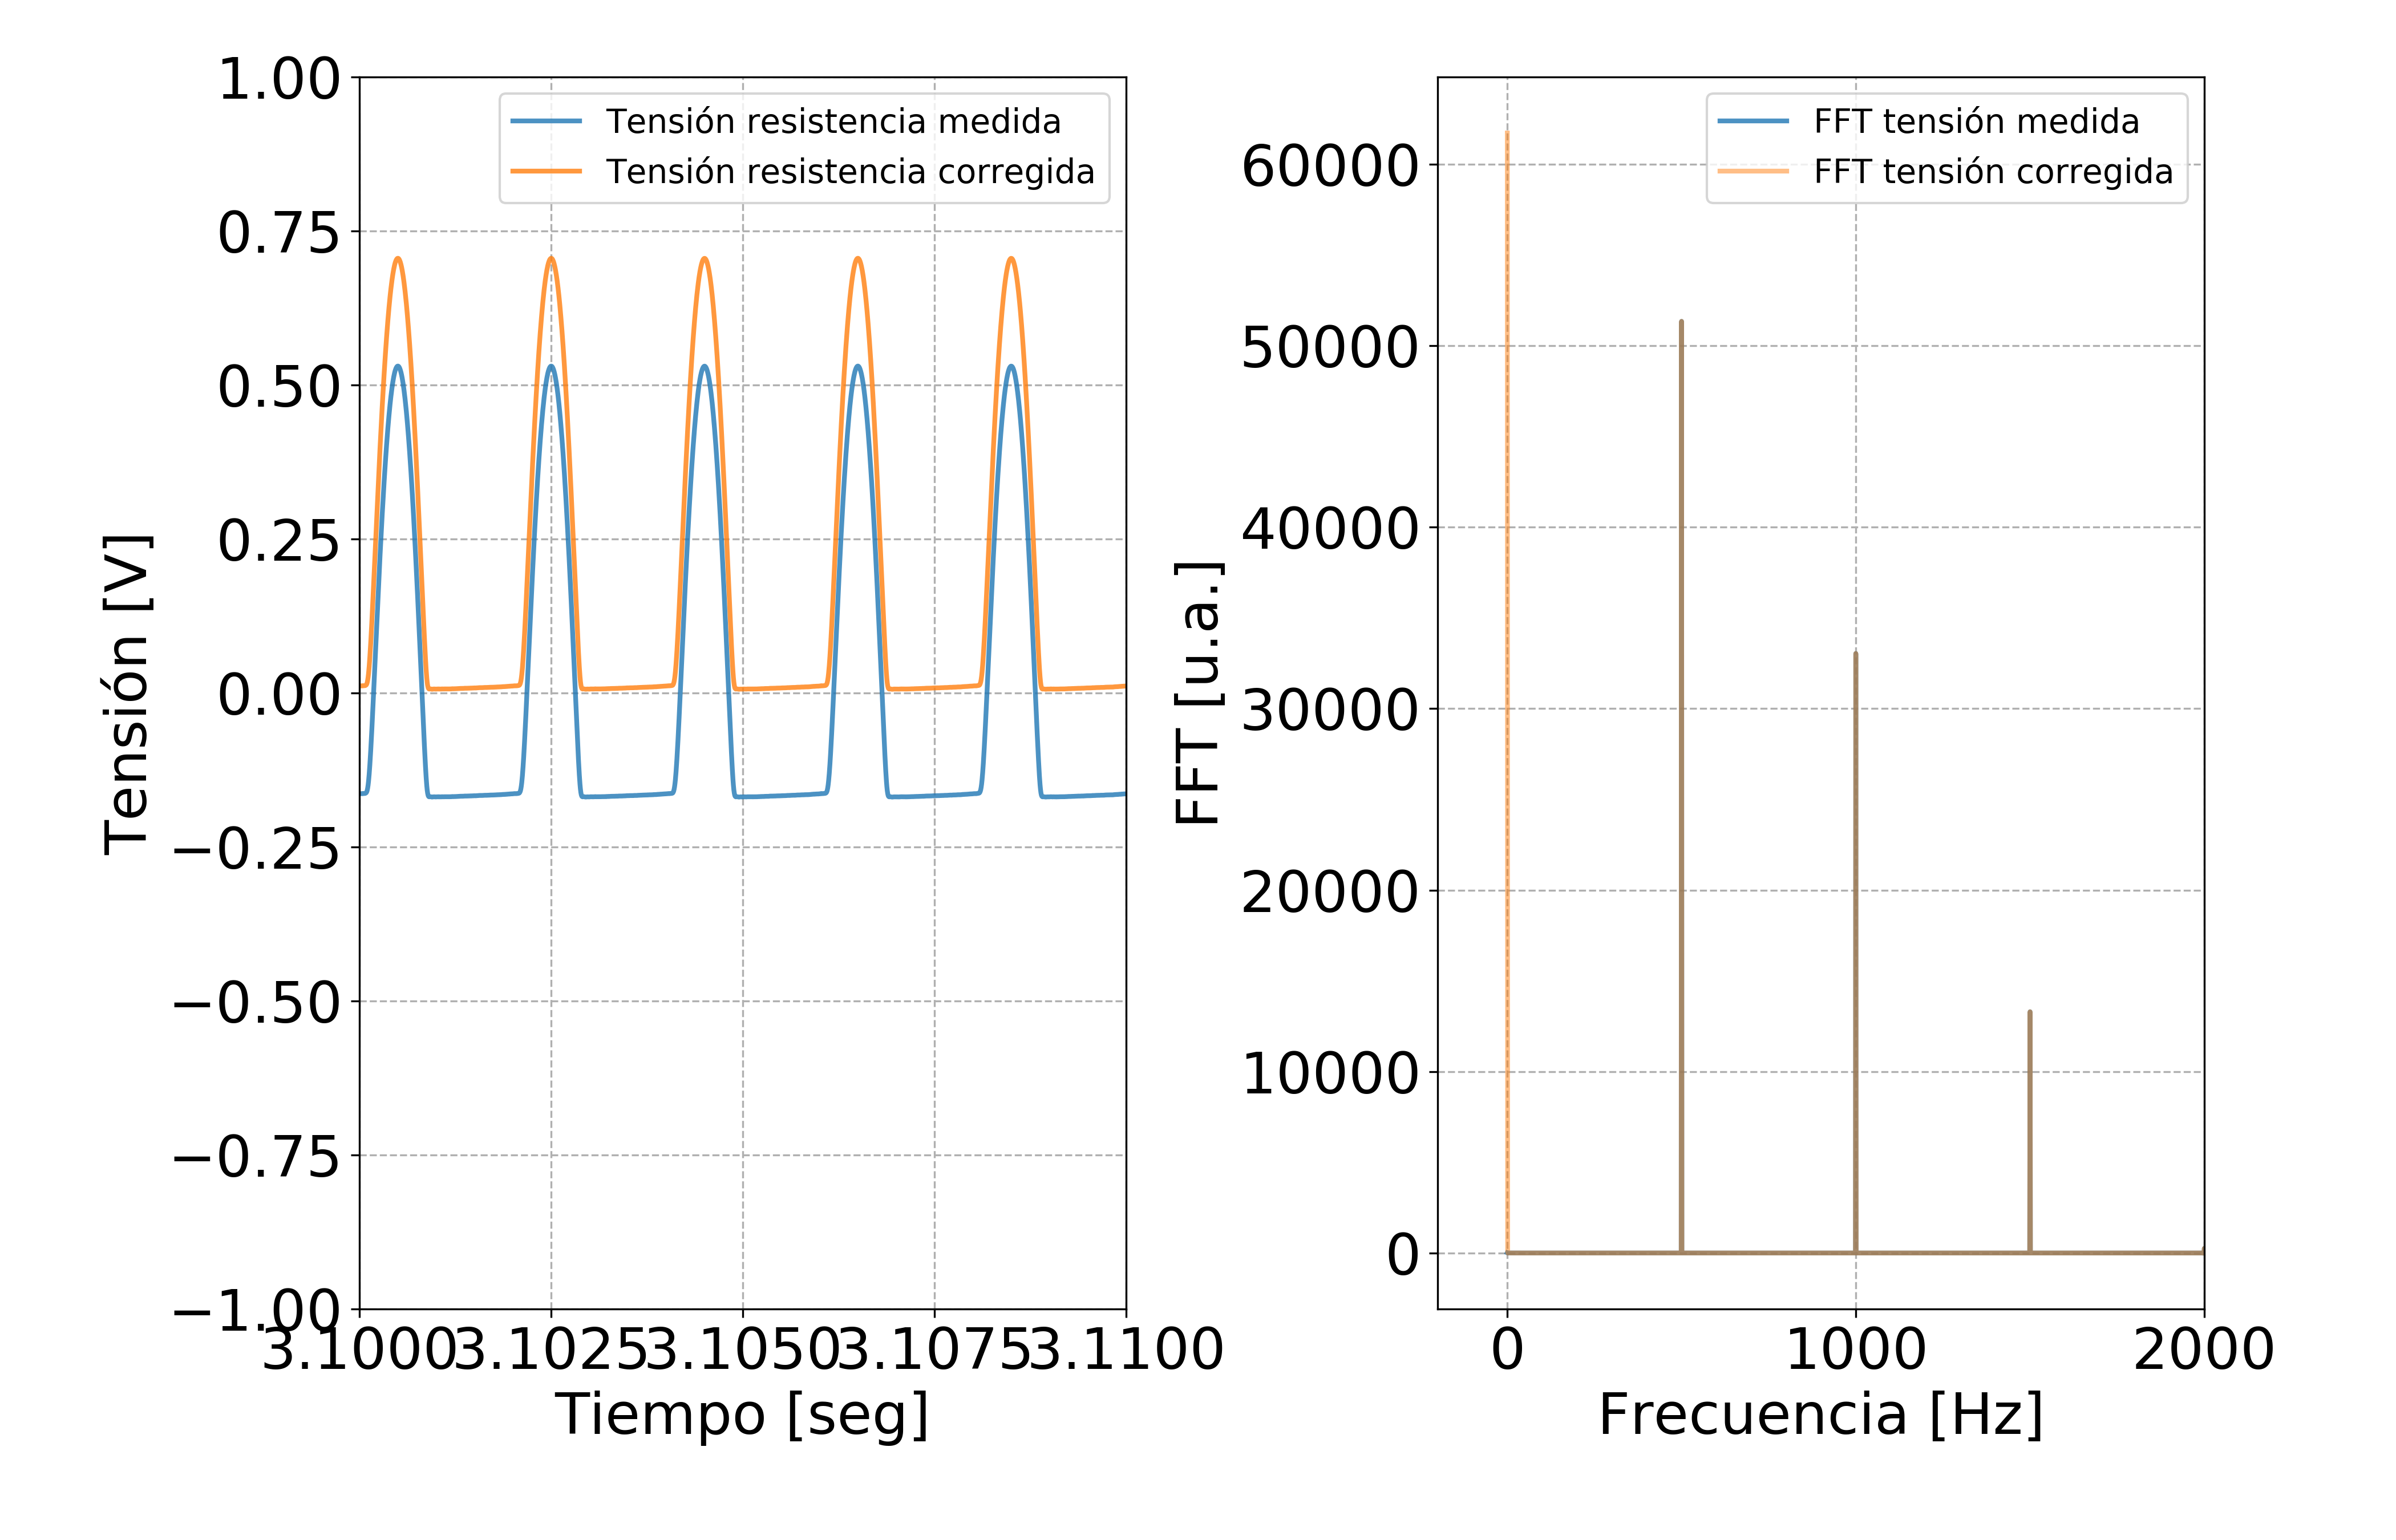
\includegraphics[scale=0.45]{caida_diodo_res_1N4007_82_20C_500hz_fft.png}
\caption{Corrimiento en tensión debido a limitaciones en el ancho de banda. Al corregir la señal estamos agregando una componente de frecuencia 0 Hz (componente continua) que es recortada por la entrada. \label{fig:caida_diodo_res_1N4007_82_20C_500hz_fft}}
\end{figure} 

\begin{figure} [H]
\centering
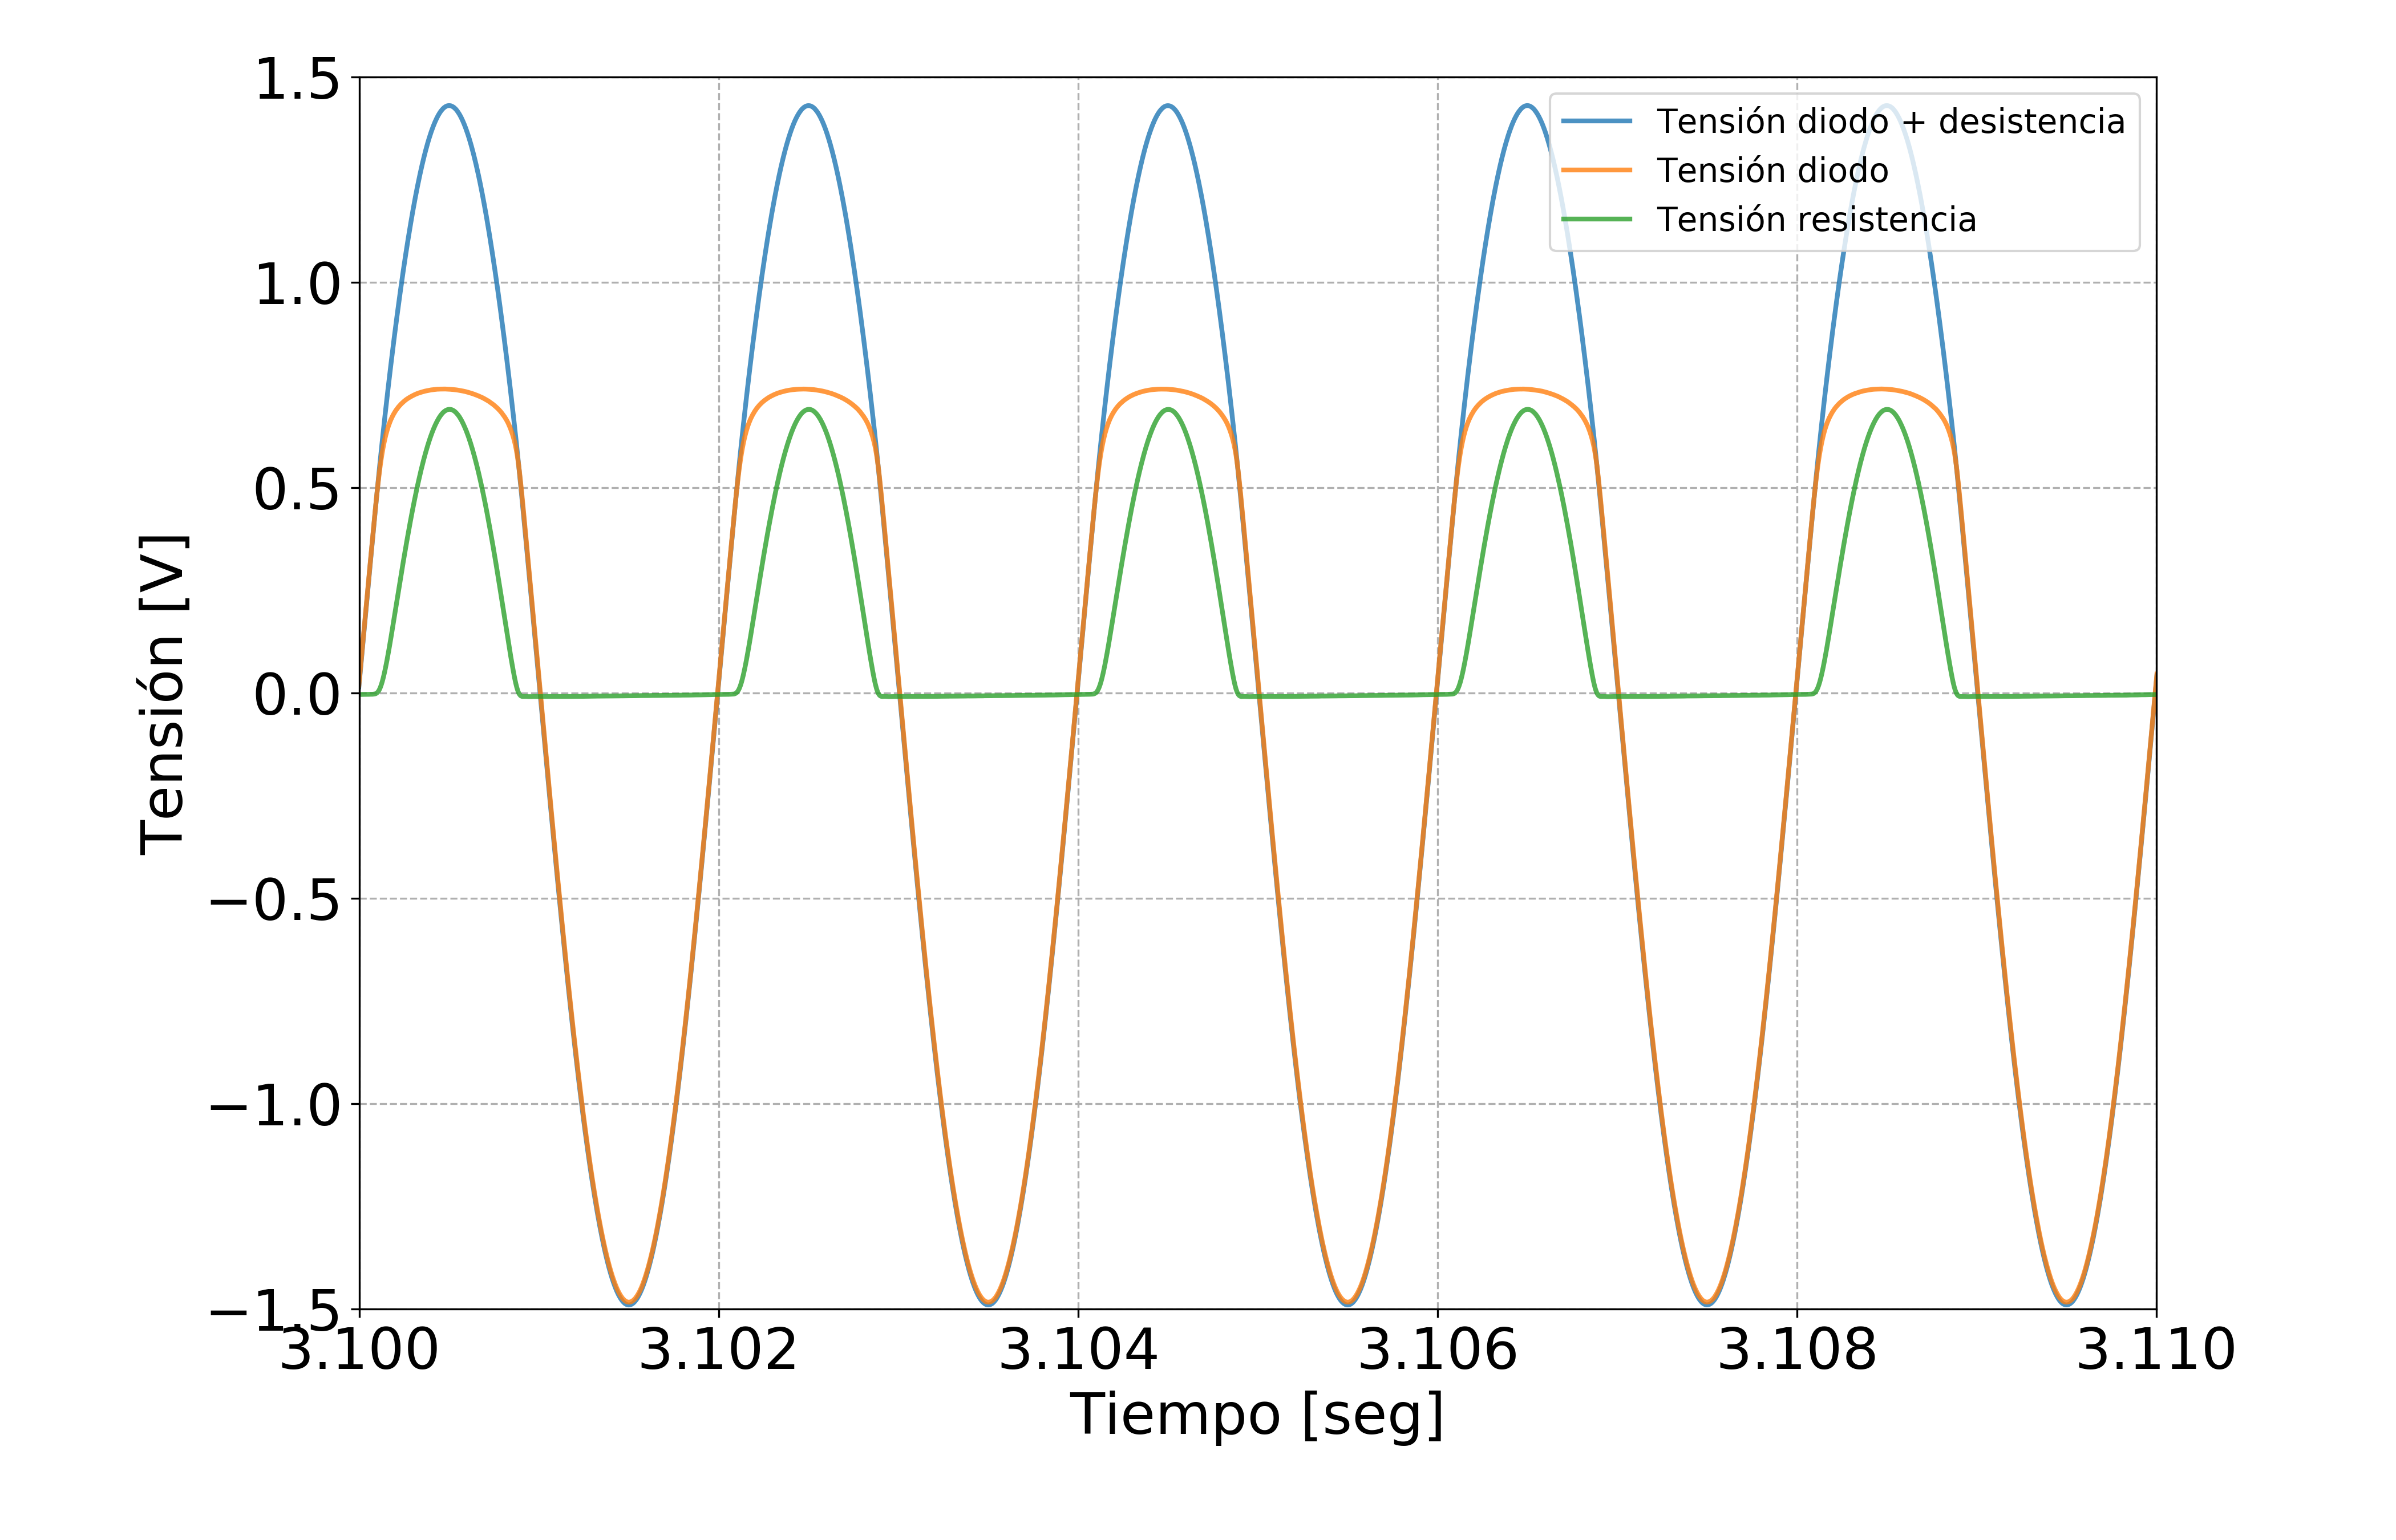
\includegraphics[scale=0.45]{caida_diodo_res_1N4007_82_20C_500hz.png}
\caption{Corrimiento en tensión debido a limitaciones en el ancho de banda. Al corregir la señal estamos agregando una componente de frecuencia 0 Hz (componente continua) que es recortada por la entrada. \label{fig:caida_diodo_res_1N4007_82_20C_500hz}}
\end{figure} 

Con la caída de tensión en la resistencia obtenemos la corriente y entonces podemos realizar curva I-V del diodo (Figura \ref{fig:curva_diodo_1N4007_82_20C_500hz}). En el gráfico mostramos la curva del diodo obtenida al considerar por un lado los flancos positivos de tensión de polarización y por el otro los flancos negativos, observándose histéresis en la curva I-V. 

\begin{figure} [H]
\centering
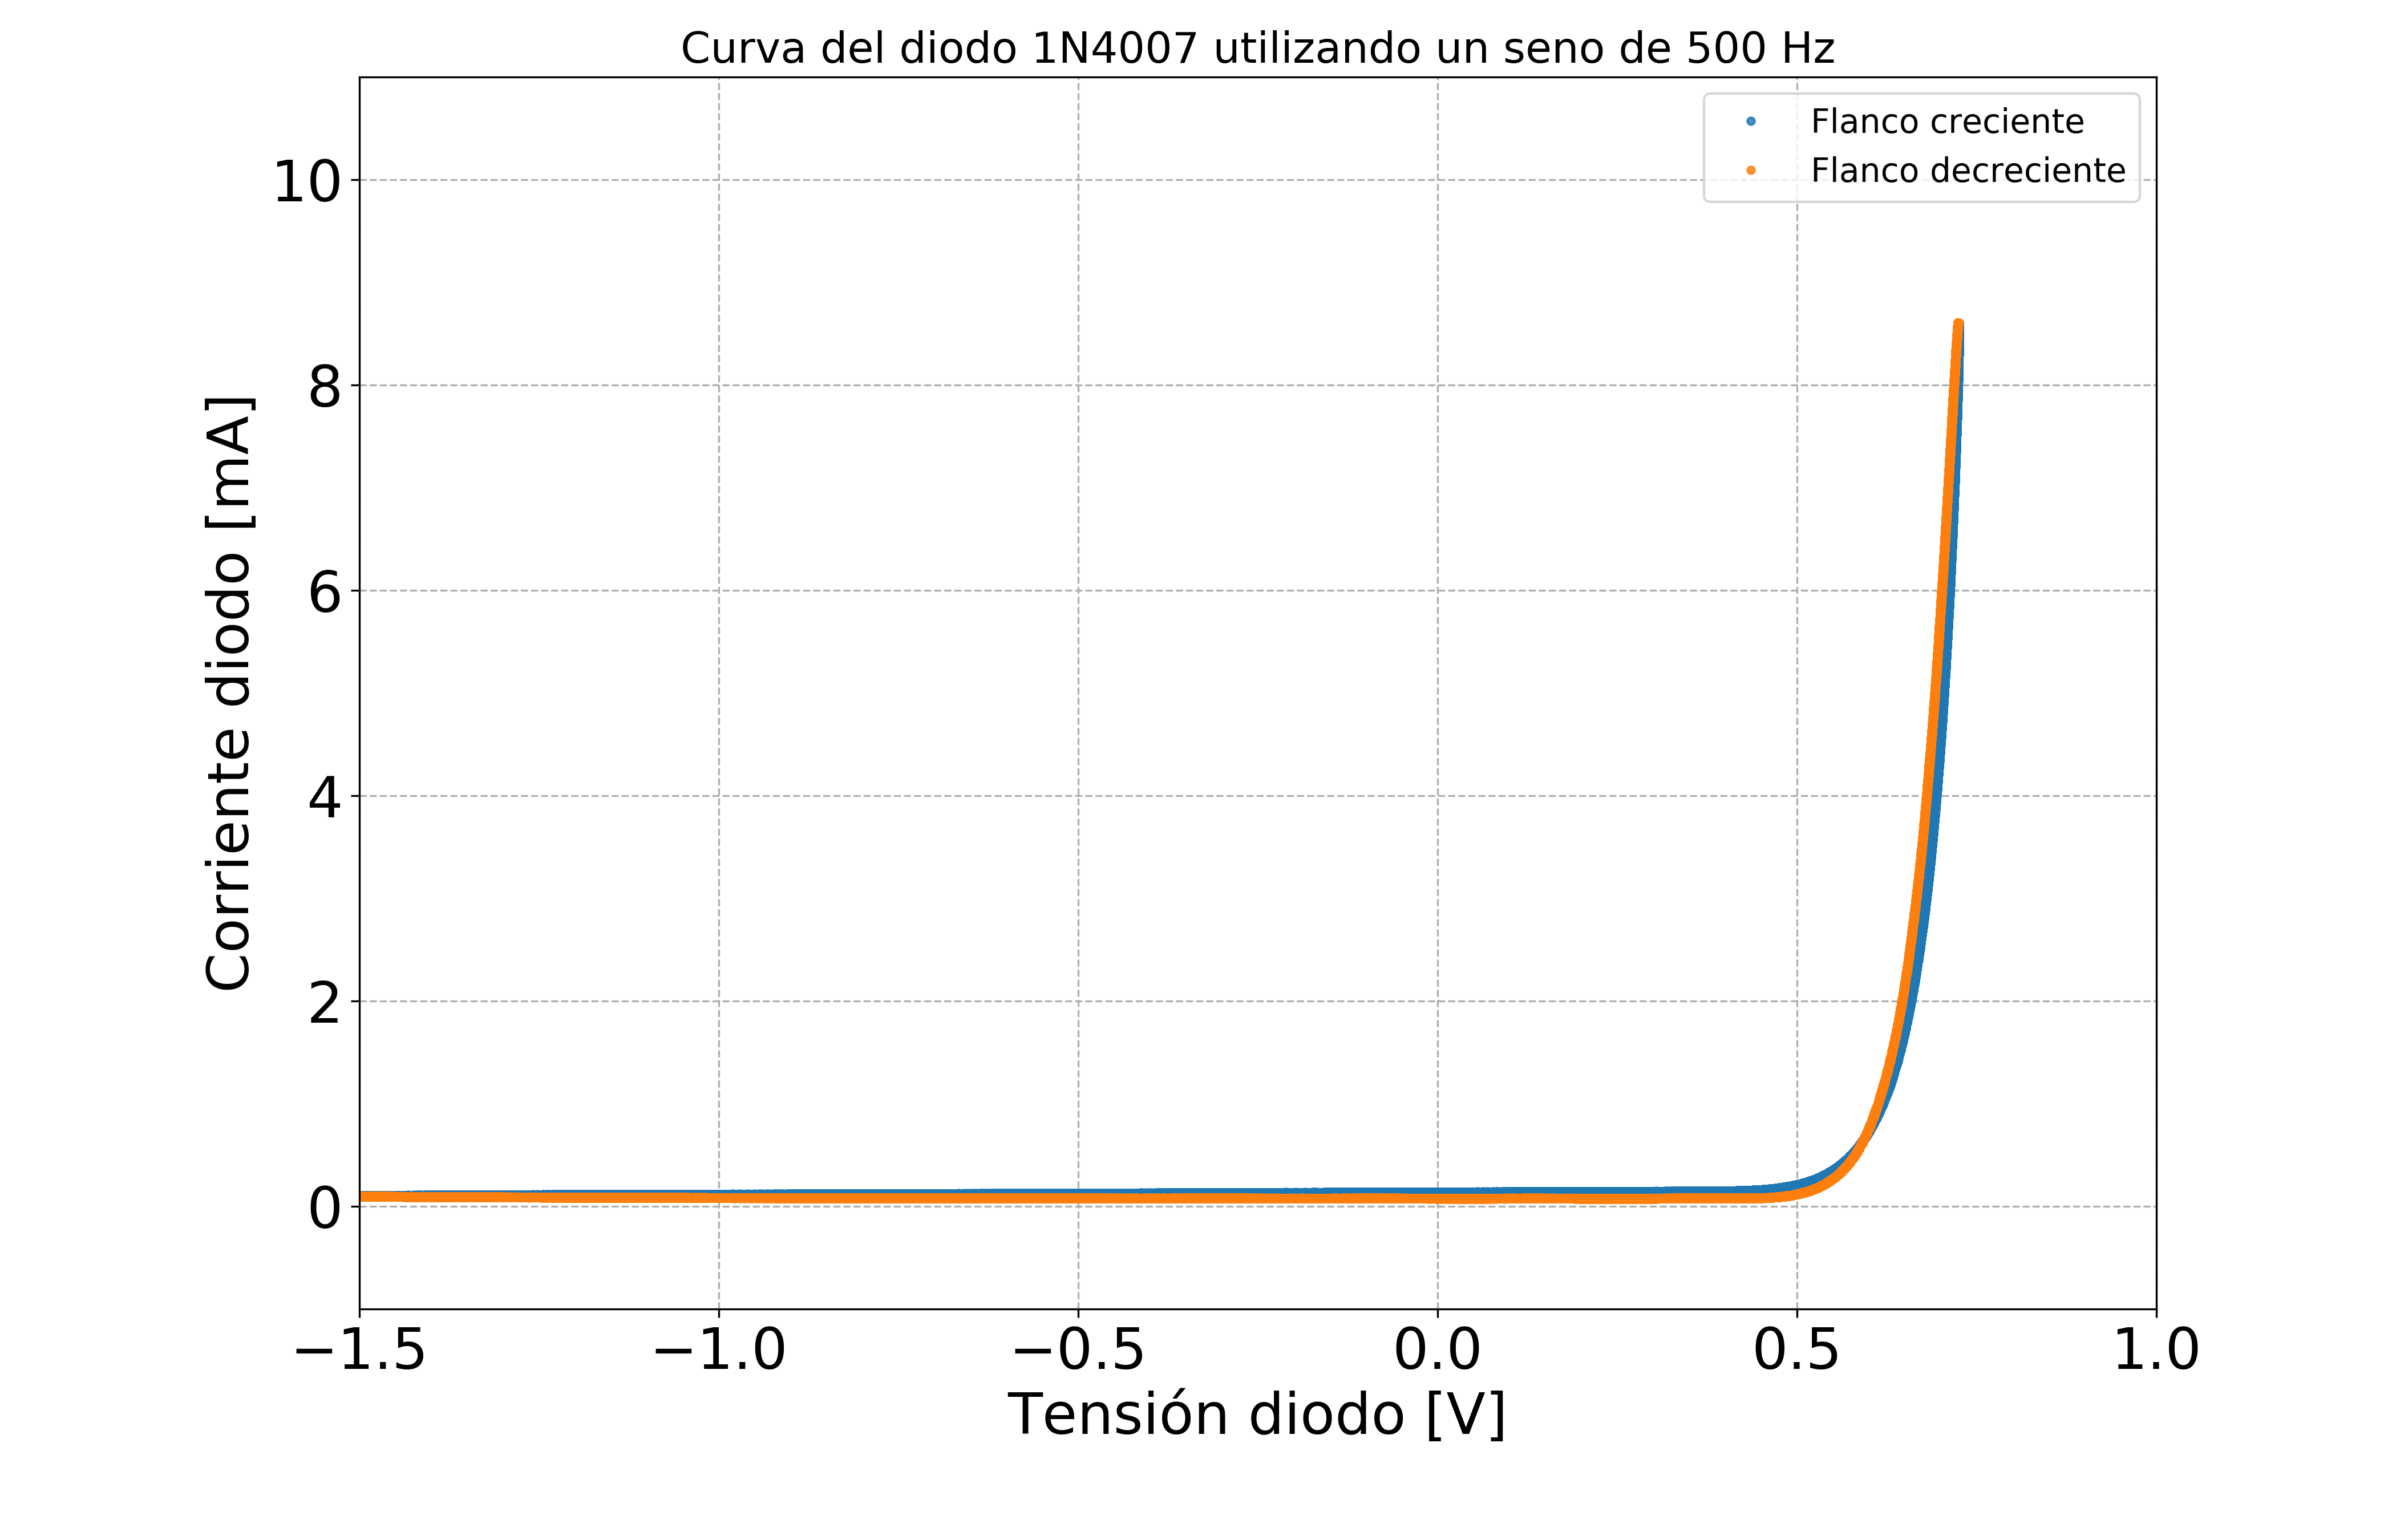
\includegraphics[scale=0.45]{curva_diodo_1N4007_82_20C_500hz.png}
\caption{Curva I-V de diodo 1N4007. Se observa histéresis entre el la medición correspondiente al flanco de tensión positivo y negativo. \label{fig:curva_diodo_1N4007_82_20C_500hz}}
\end{figure} 

%\begin{figure} [H]
%\centering
%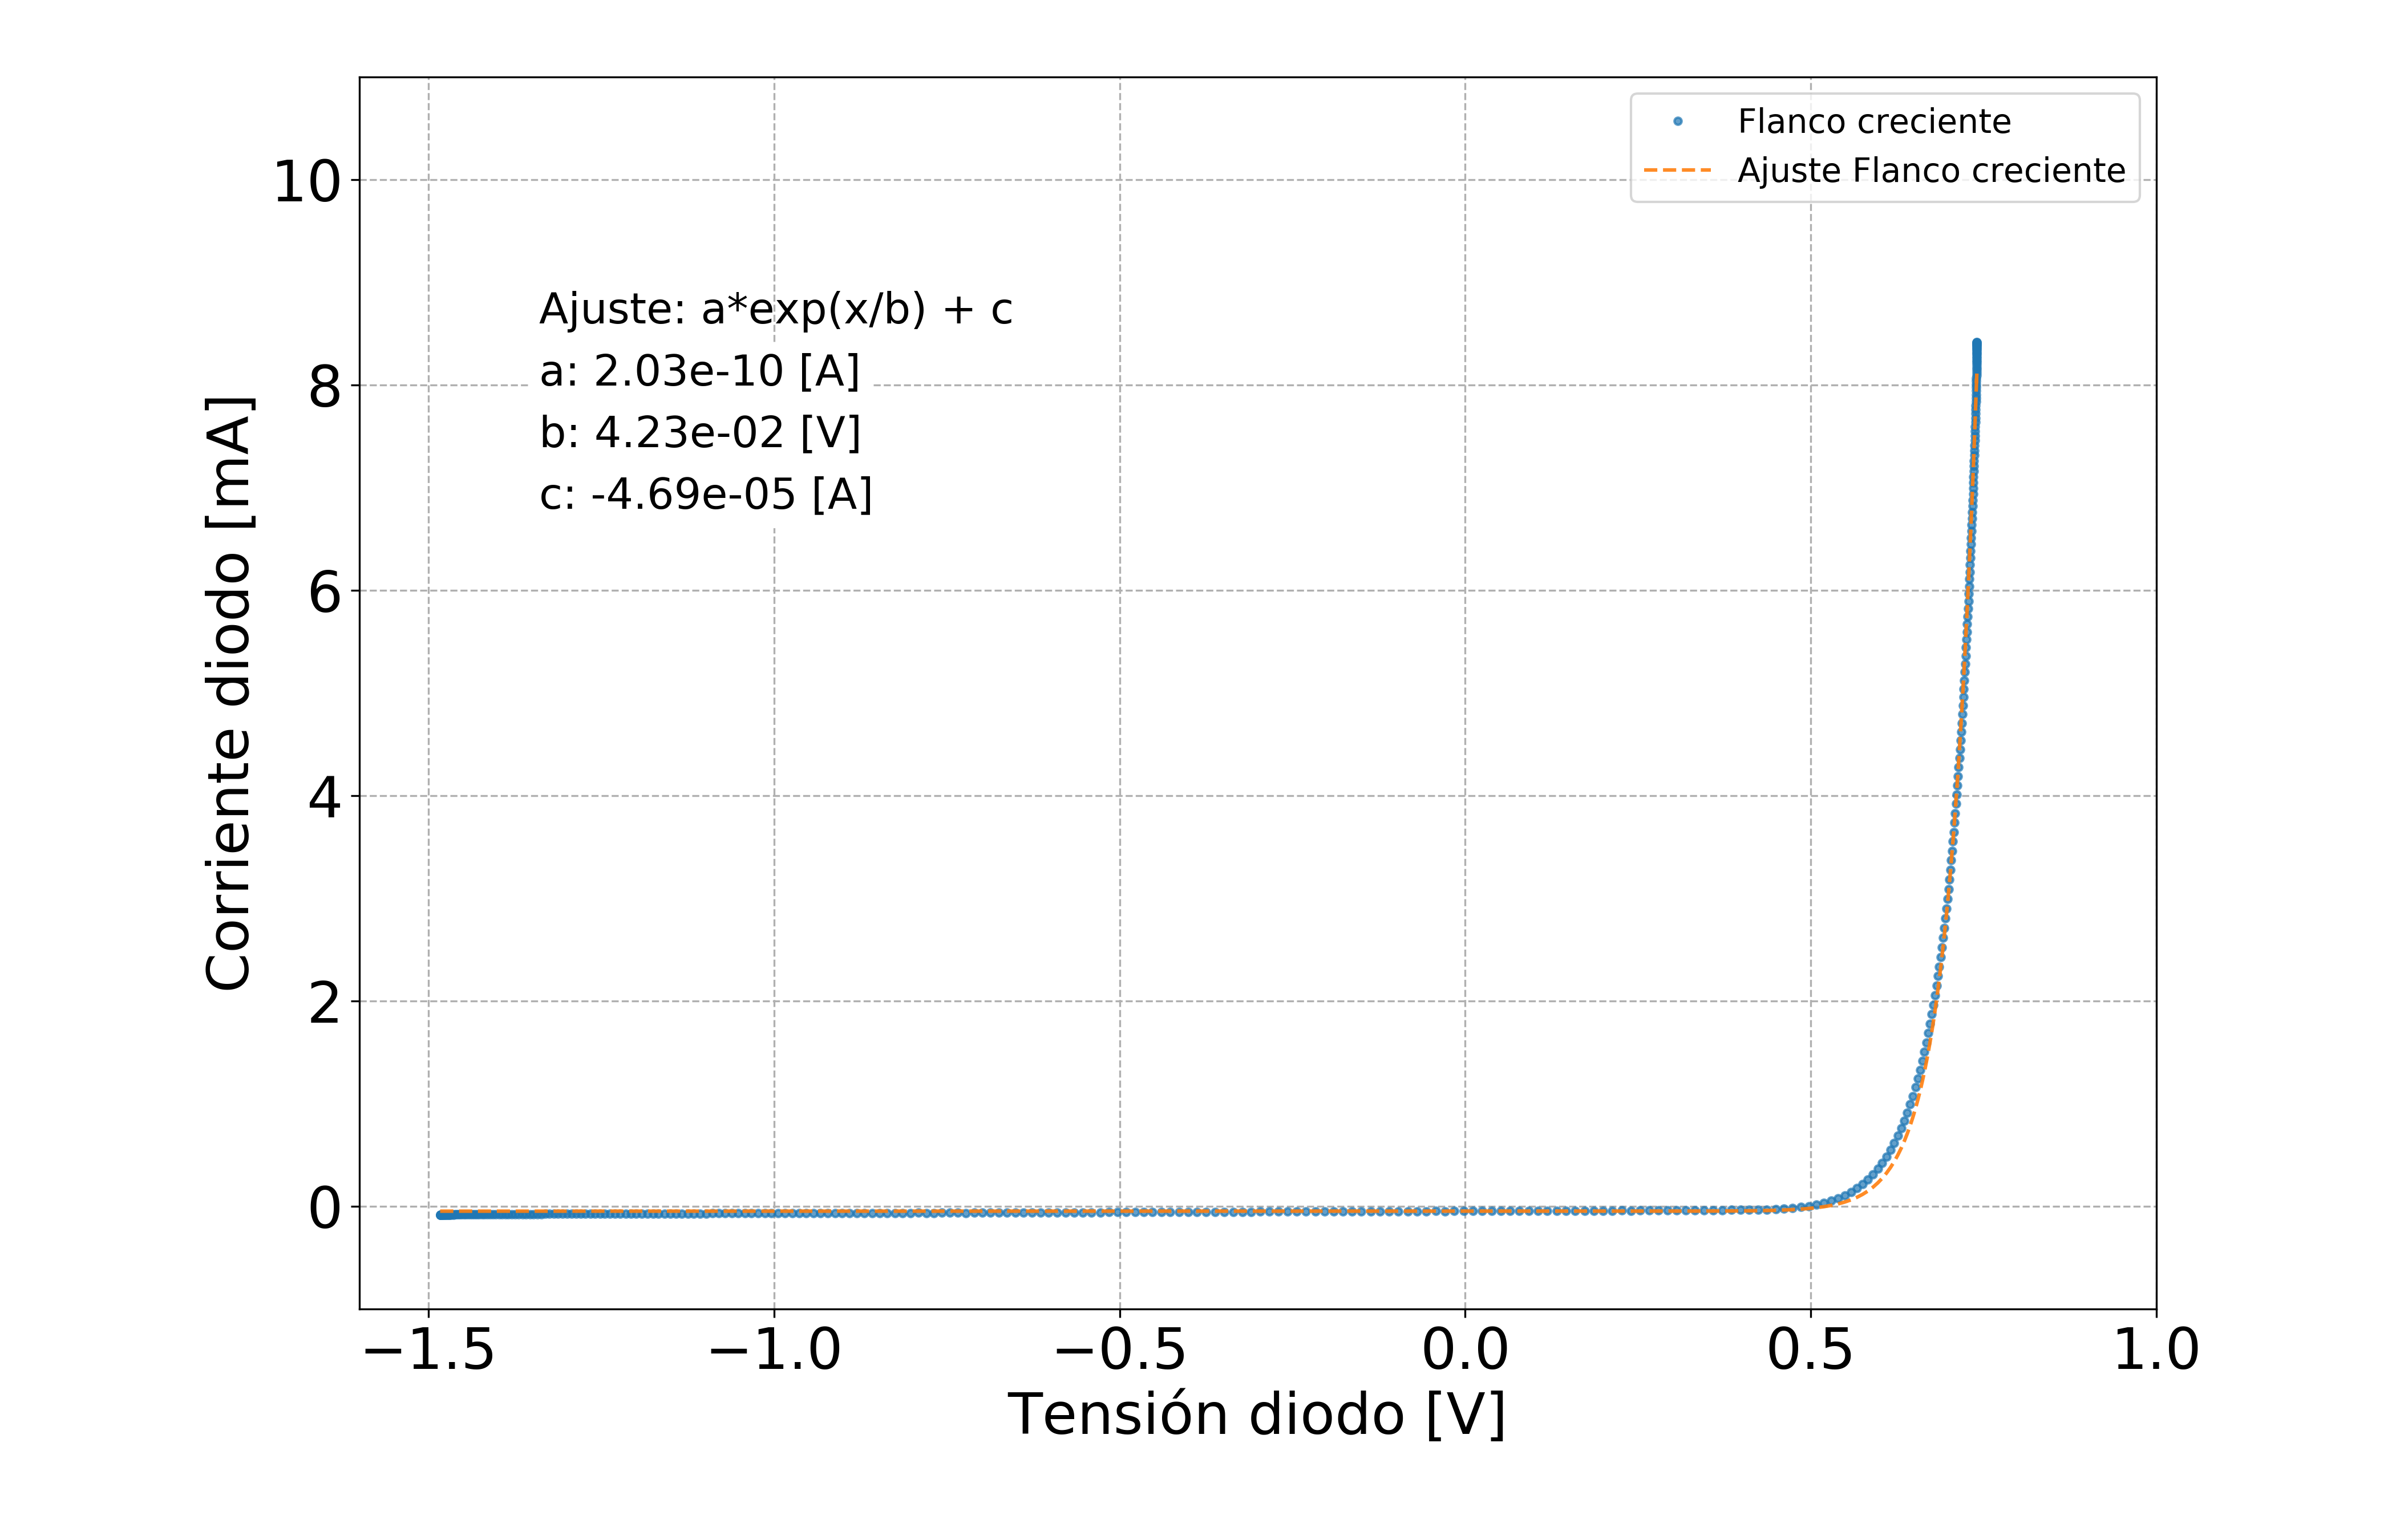
\includegraphics[scale=0.45]{ajuste_diodo_1N4007_82_20C_500hz.png}
%\caption{Ajuste exponencial de la curva I-V correspondiente al flanco positivo de tensión. \label{fig:ajuste_diodo_1N4007_82_20C_500hz}}
%\end{figure} 


\subsection*{Factor de idealidad n}
A continuación nos propusimos medir el factor de idealidad  del diodo (n) a partir de variar la temperatura del diodo. Si tenemos en cuenta el modelo del diodo vemos que el umbral de polarización depende de la temperatura según la siguiente relación:
\[
I=I_S(e^{V_D/nV_T}-1)
\]

Donde:
\[
V_T=\frac{KT}{q}
\]

Donde $K$ es la constante de Boltzmann, $T$ la temperatura del diodo, y $q$ la carga del electrón. Por lo tanto al aumentar la temperatura esperamos observar una disminución del umbral de polarización. Luego ajustamos los resultados a la curva del diodo y estimamos el valor de n.
Para variar la temperatura del diodo se dispuso una fuente de corriente con control PI diseñada para estabilizar la temperatura al utilizar celdas Peltiers. La fuente modelo Wavelength 3293, utiliza un termistor de 10K para medir la temperatura, y dispone de una entrada ($V_{set}$) para fijar la temperatura deseada y dos salidas de tensión para monitorear las temperaturas fijada ($T_{set}$) y actual ($T_{act}$). Para la conversión de tensión a temperatura, necesaria para determinar $V_{set}$ $T_{set}$ y $T_{act}$, se utilizan los coeficientes de Steinhart del termistor y la corriente de bias ($I_{bias}$) fijada en el termistor  de 100  ${\mu A}$. Para ello basta considerar la ecuación del Steinhart del termistor:

\[
\frac{1}{T} = A + B\ln(R)+ C[\ln(R)]^3
\]

Donde T es la temperatura, y ,A B C los coeficientes de Steinhart del termistor.

\[
\frac{1}{T_{set,act}} = A + B\ln(\frac{V_{set,act}}{I_{bias}})+ C[\ln(\frac{V_{set,act}}{I_{bias}})]^3
\]

De esta manera relacionamos las tensiones actual y fijada ($V_{act}$ y $V_{set}$) con las temperaturas actual y fijada ($T_{act}$ y $T_{set}$). Para el control del experimento se utilizó una Arduino Due que permitió tanto la medición de la tensión actual ($V_{act}$) como la el ajuste de la tensión deseada ($V_{set}$) a partir de la salida digital-analógica DAC0.  La comunicación entre la Arduino Due y la PC se realizó con la librería PySerial. En la Figura \ref{fig:esquema_temp} se muestra un esquema del dispositivo experimental.

\begin{figure} [H]
\centering
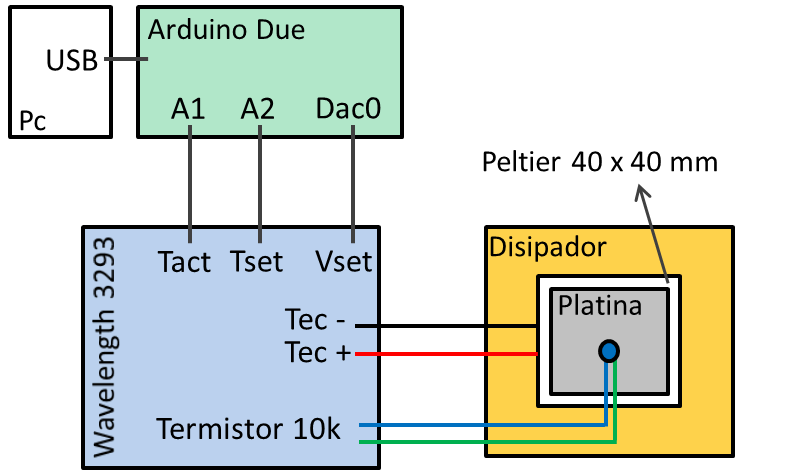
\includegraphics[scale=0.75]{esquema_temp.png}
\caption{ Esquema del dispositivo experimental. \label{fig:esquema_temp}}
\end{figure} 

En la Figura \ref{fig:esquema_arduino} se muestra un esquema del programa de control y adquisición del dispositivo experimental. En Python se fija la temperatura deseada ($T_{set}$) y se manda al buffer de la arduino quien lee la temperatura enviada. La arduino fija la tensión correspondiente  ($V_{set}$) utilizando la ecuación de Steinhart y la manda a la salida DAC0. La arduino además mide las tensiones $V_{act}$ y $V_{set}$, y las envia a Python con la temperatura $T_{set}$ leida. Cuando la temperatura leida por Python es la misma a la enviada, se esperan 2 minutos  a que la temperatura $T_{act}$ se estabilice en el valor $T_{set}$ y se realiza la medición de la curva I-V con la placa de audio (guardando el valor $T_{act}$ asignado a la medición). Luego se fija un nuevo valor de temperatura  $T_{set}$ y se repite el proceso, hasta terminar todo el barrido de temperaturas. En nuestro caso se realizó un barrido de \SI{10}{\celsius}  a \SI{38}{\celsius} cada \SI{2}{\celsius}.

\begin{figure} [H]
\centering
\includegraphics[scale=0.75]{esquema_arduino.png}
\caption{ Esquema del programa de control. \label{fig:esquema_arduino}}
\end{figure} 

En la Figura \ref{fig:curva_diodo_creciente_temperatura} se muestran las curvas I-V del diodo 1N4007 para las distintas temperaturas correspondientes al flanco positivo al enviar una señal sinusoidal de 1000 Hz.Como era esperable se observa una disminución del umbral de polarización a medida que se aumenta la temperatura del diodo.

\begin{figure} [H]
\centering
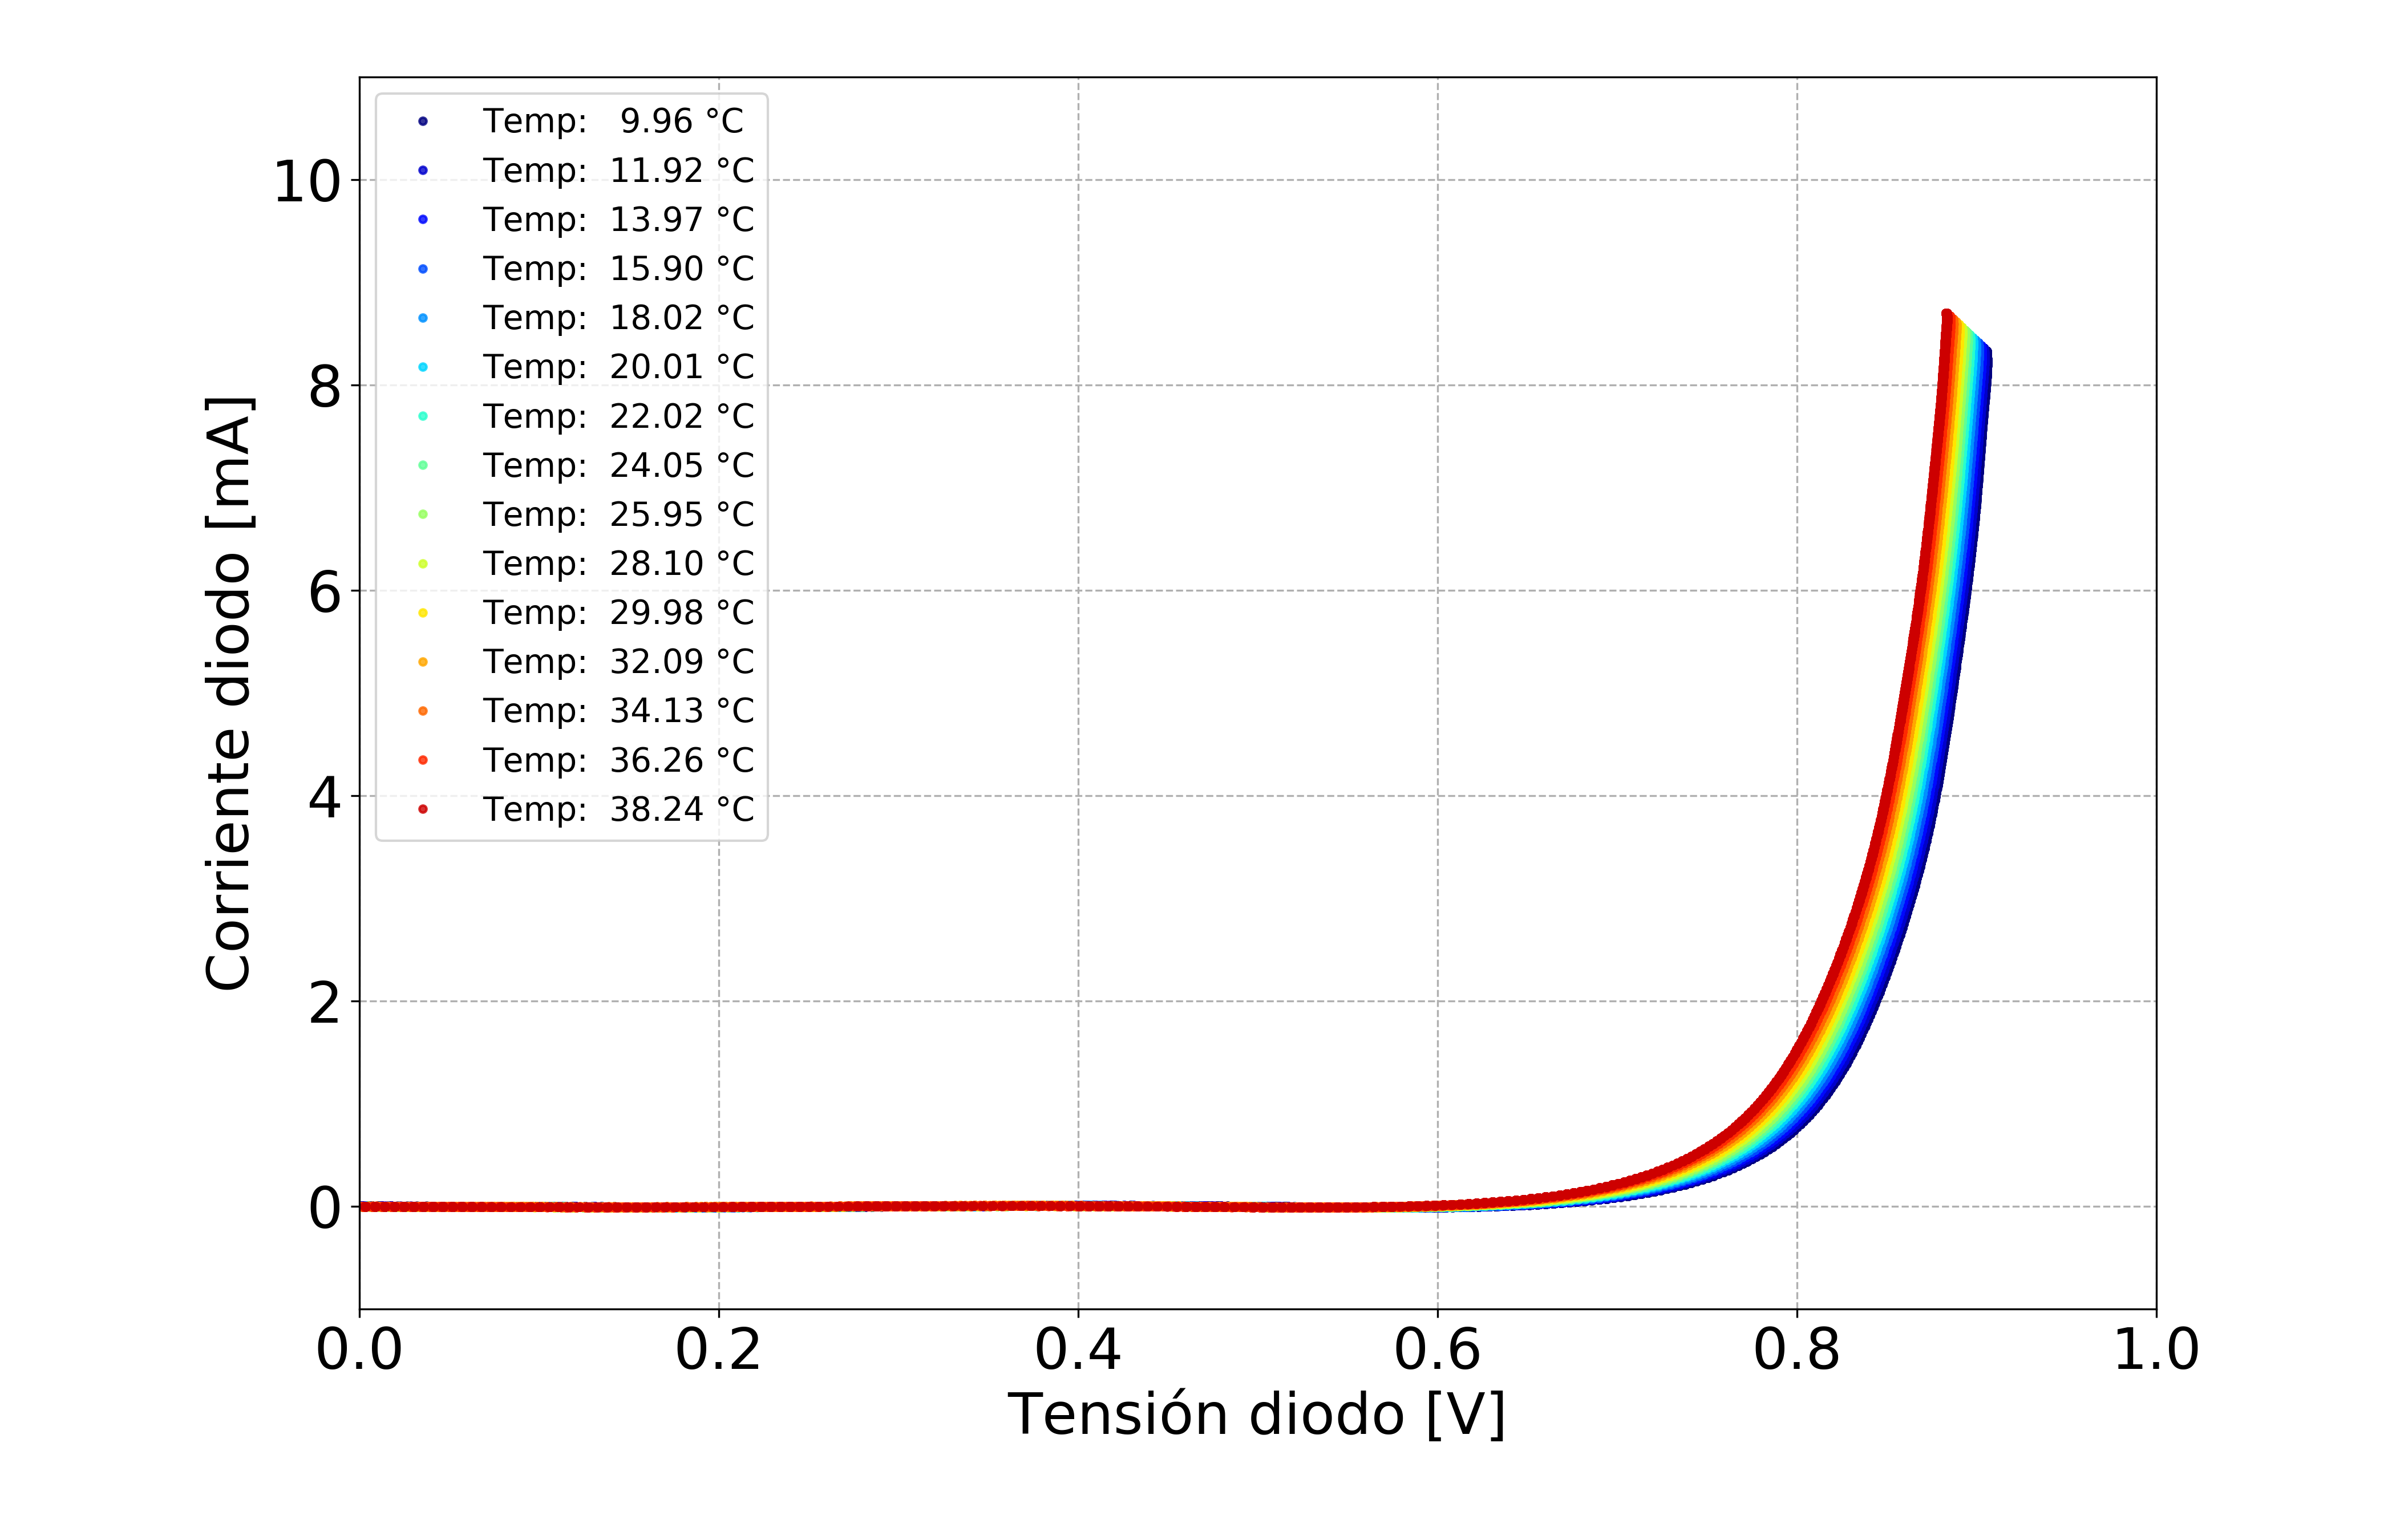
\includegraphics[scale=0.45]{curva_diodo_creciente_temperatura.png}
\caption{Curva I-V del diodo 1N4007 para distintas temperaturas. \label{fig:curva_diodo_creciente_temperatura}}
\end{figure} 

A continuación realizamos el ajuste para cada una de las curvas según el modelo del diodo mostrado más arriba. De esta manera obtenemos un valor de $V_T*q/K$ para cada valor de temperatura, que graficamos a continuación en la Figuras \ref{fig:factor_linealidad_creciente} y \ref{fig:factor_linealidad_decreciente} para el flanco positivo y negativo respectivamente. Mostramos también los ajustes lineales cuya pendiente representa el factor de idealidad n, obteniendo valores de 1.58 y 1.15 para los flancos positivos y negativos respectivamente. Cabe destacar que la ordenada al origen en ambos casos no es cero obteniendo un valor de $45 K$ y $227 K$ para los flancos positivos y negativos respectivamente.

\begin{figure} [H]
\centering
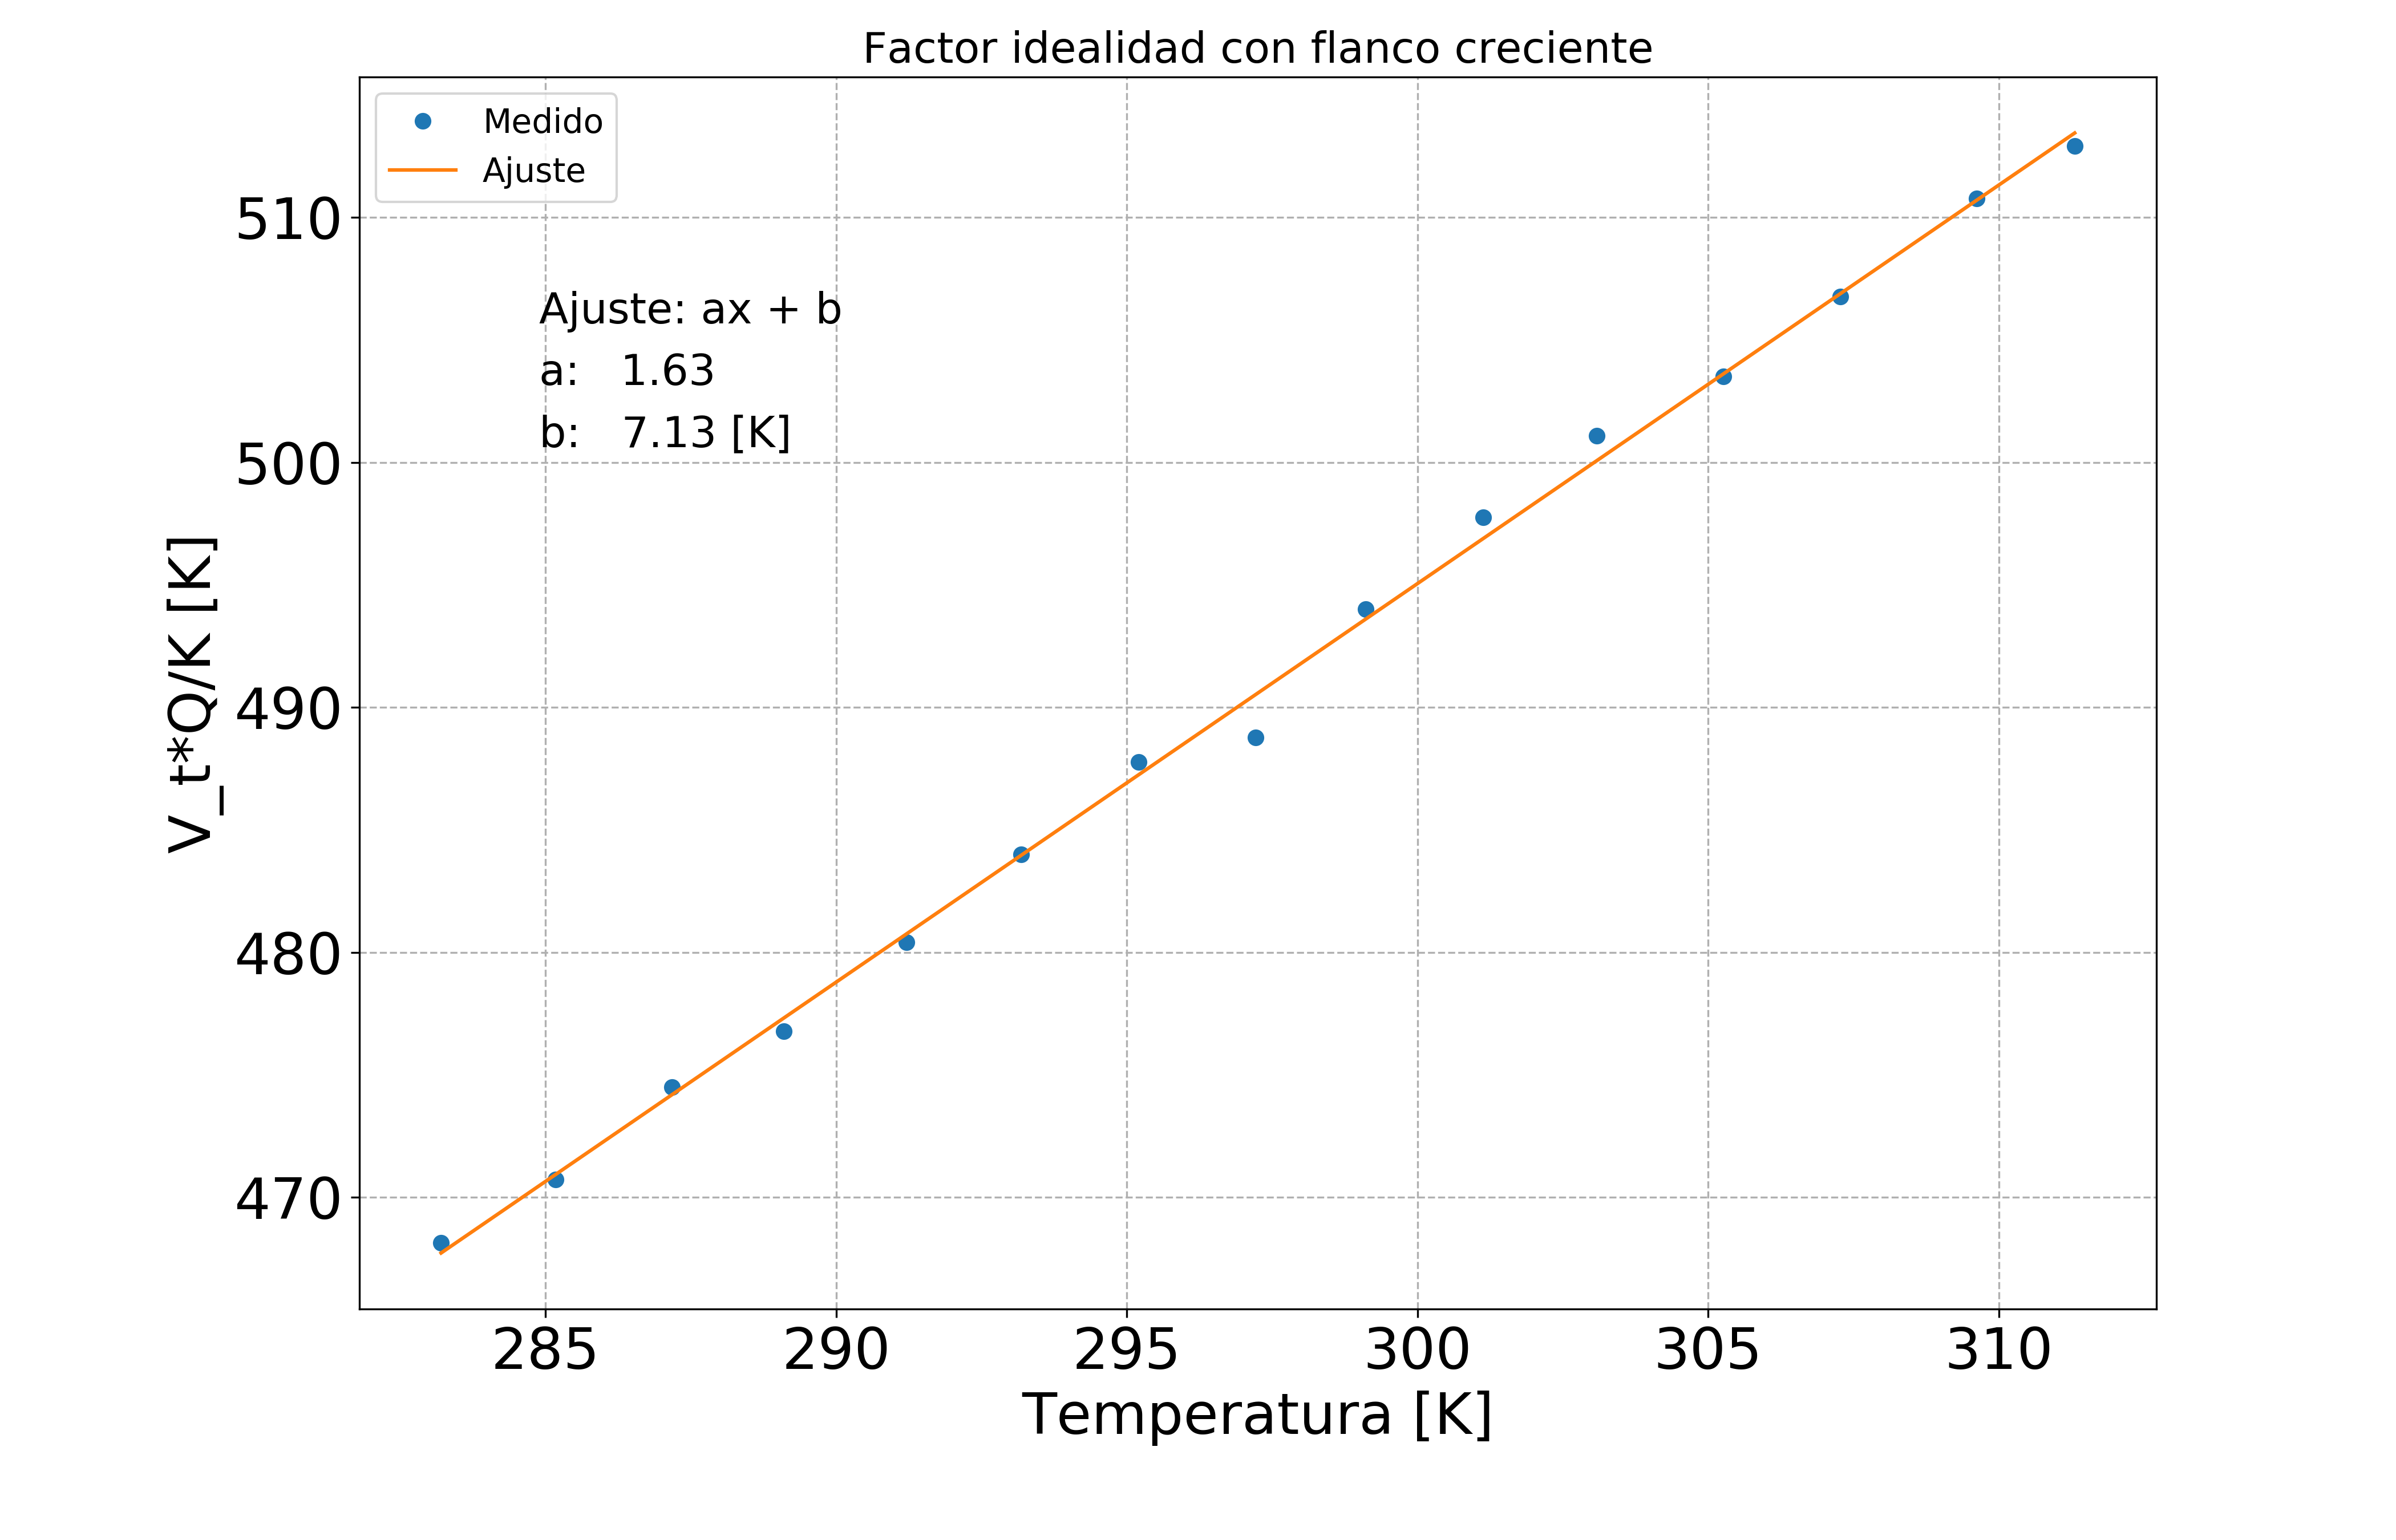
\includegraphics[scale=0.45]{factor_linealidad_creciente.png}
\caption{Factor de idealidad n del diodo 1N4007 obtenido a partir del ajuste de las curvas I-V correspondientes al flanco positivo del seno. El factor n es la pendiente del ajuste en gráfico $V_T*q/K$ vs. $ T$, en este caso n = 1.58.\label{fig:factor_linealidad_creciente}}
\end{figure} 

\begin{figure} [H]
\centering
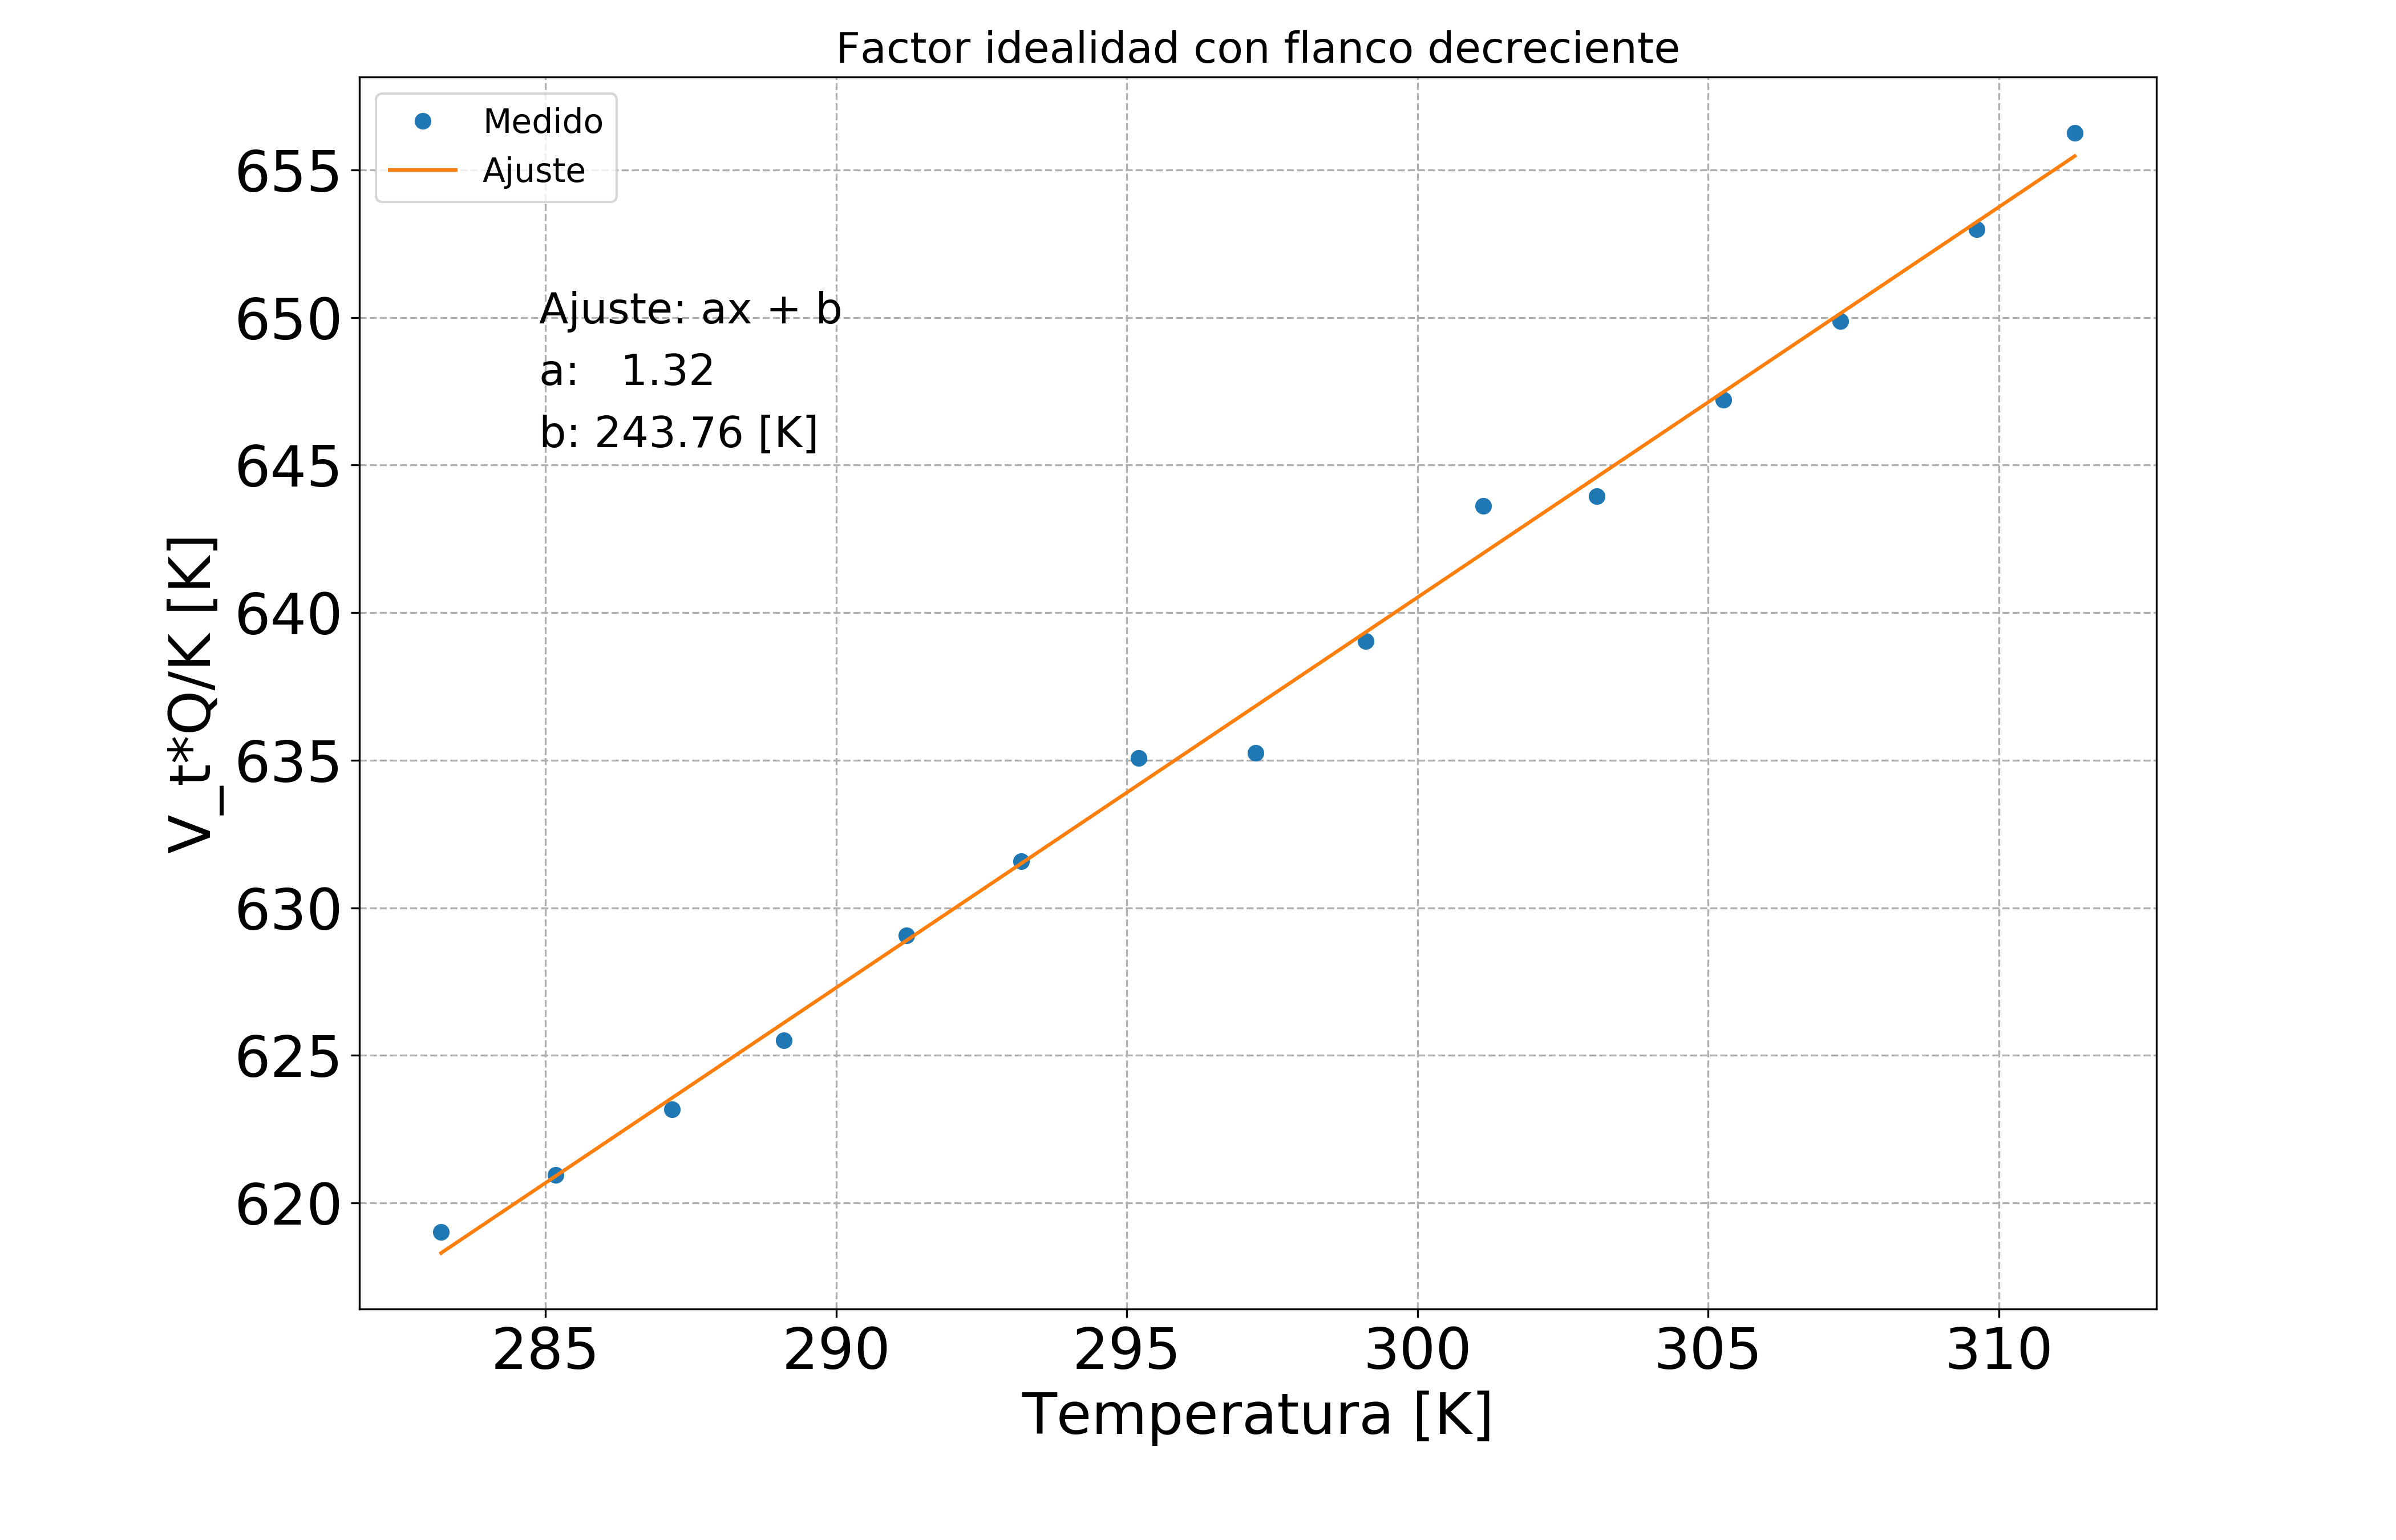
\includegraphics[scale=0.45]{factor_linealidad_decreciente.png}
\caption{Factor de idealidad n del diodo 1N4007 obtenido a partir del ajuste de las curvas I-V correspondientes al flanco negativo del seno.  El factor n es la pendiente del ajuste en gráfico $V_T*q/K$ vs. $ T$, en este caso n = 1.15.\label{fig:factor_linealidad_decreciente}}
\end{figure} 



\subsection*{Op-amp}

%\subsubsection*{Seguidor}
%\begin{figure} [H]
%\centering
%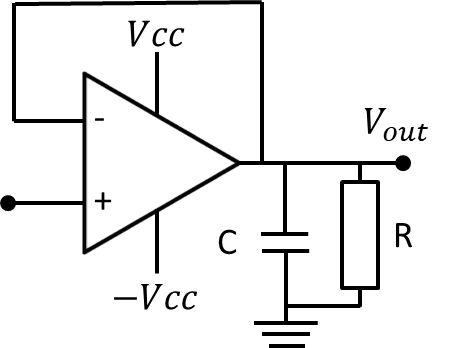
\includegraphics[scale=0.75]{seguidor.png}
%\caption{ Esquema seguidor\label{fig:seguidor}}
%\end{figure} 
%
%\begin{figure} [H]
%\centering
%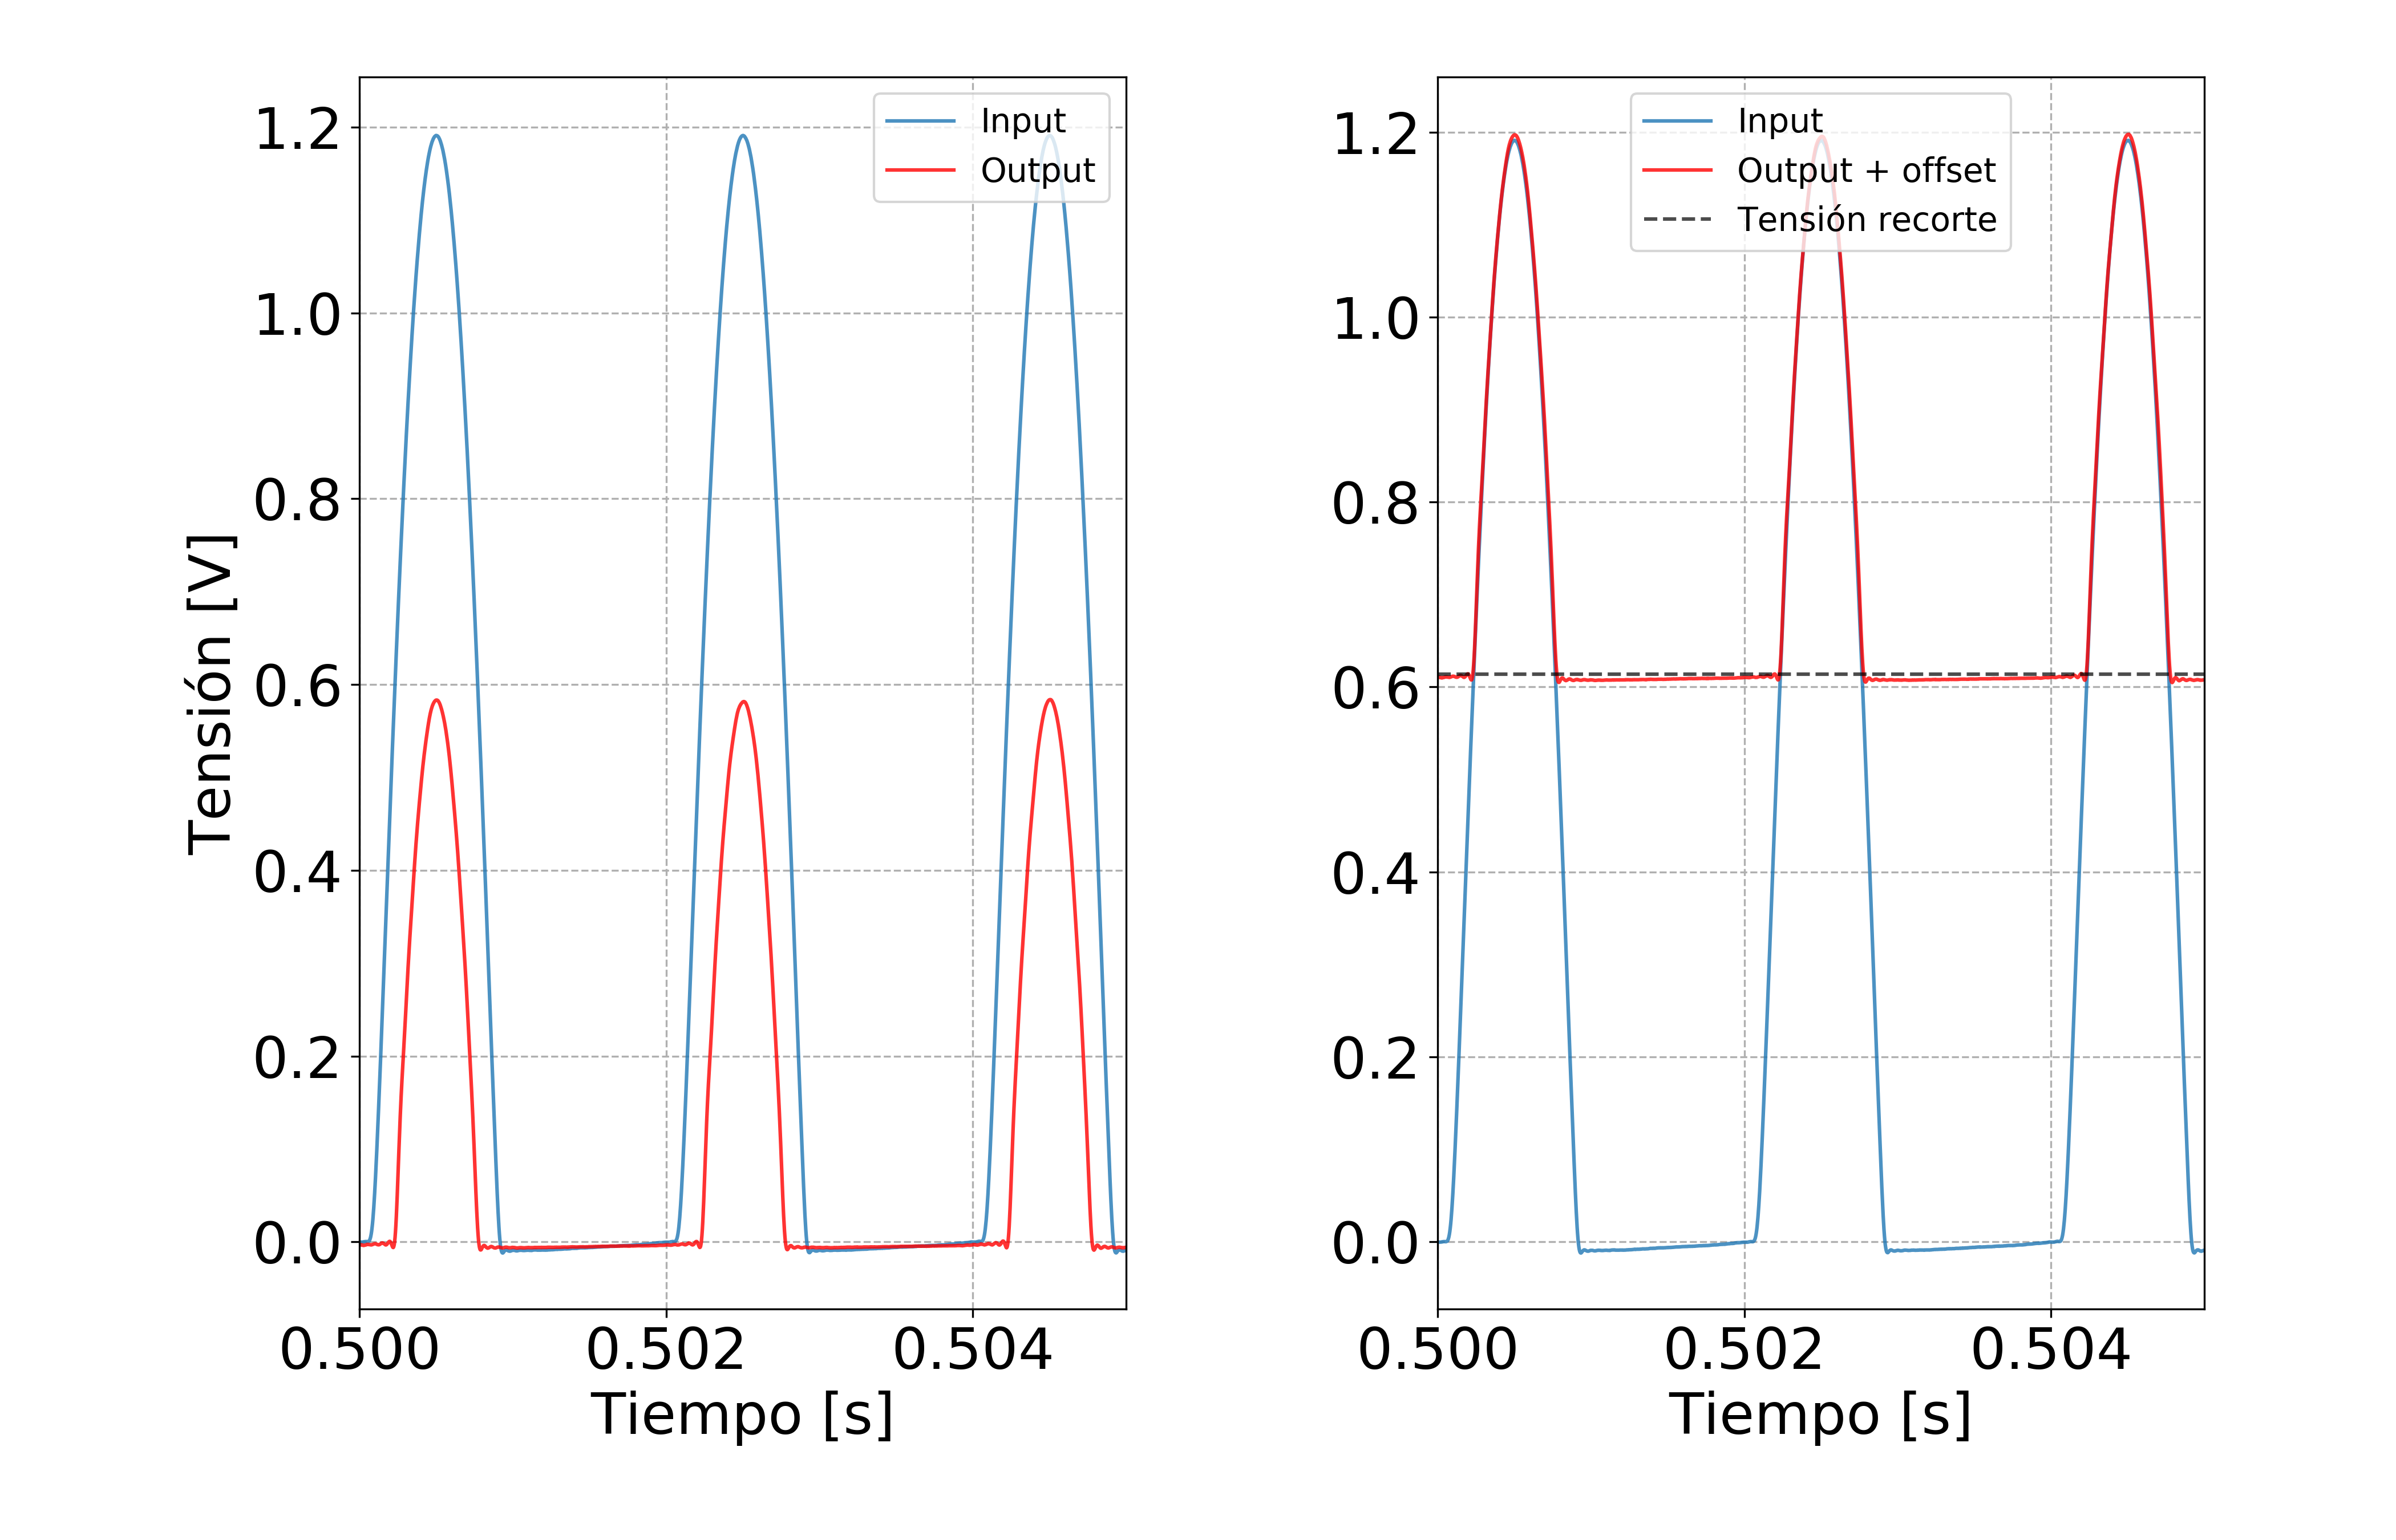
\includegraphics[scale=0.45]{salida_diodo_recortada.png}
%\caption{ Seguidor alimentado con 0 V\label{fig:salida_diodo_recortada}}
%\end{figure} 
%
%\begin{figure} [H]
%\centering
%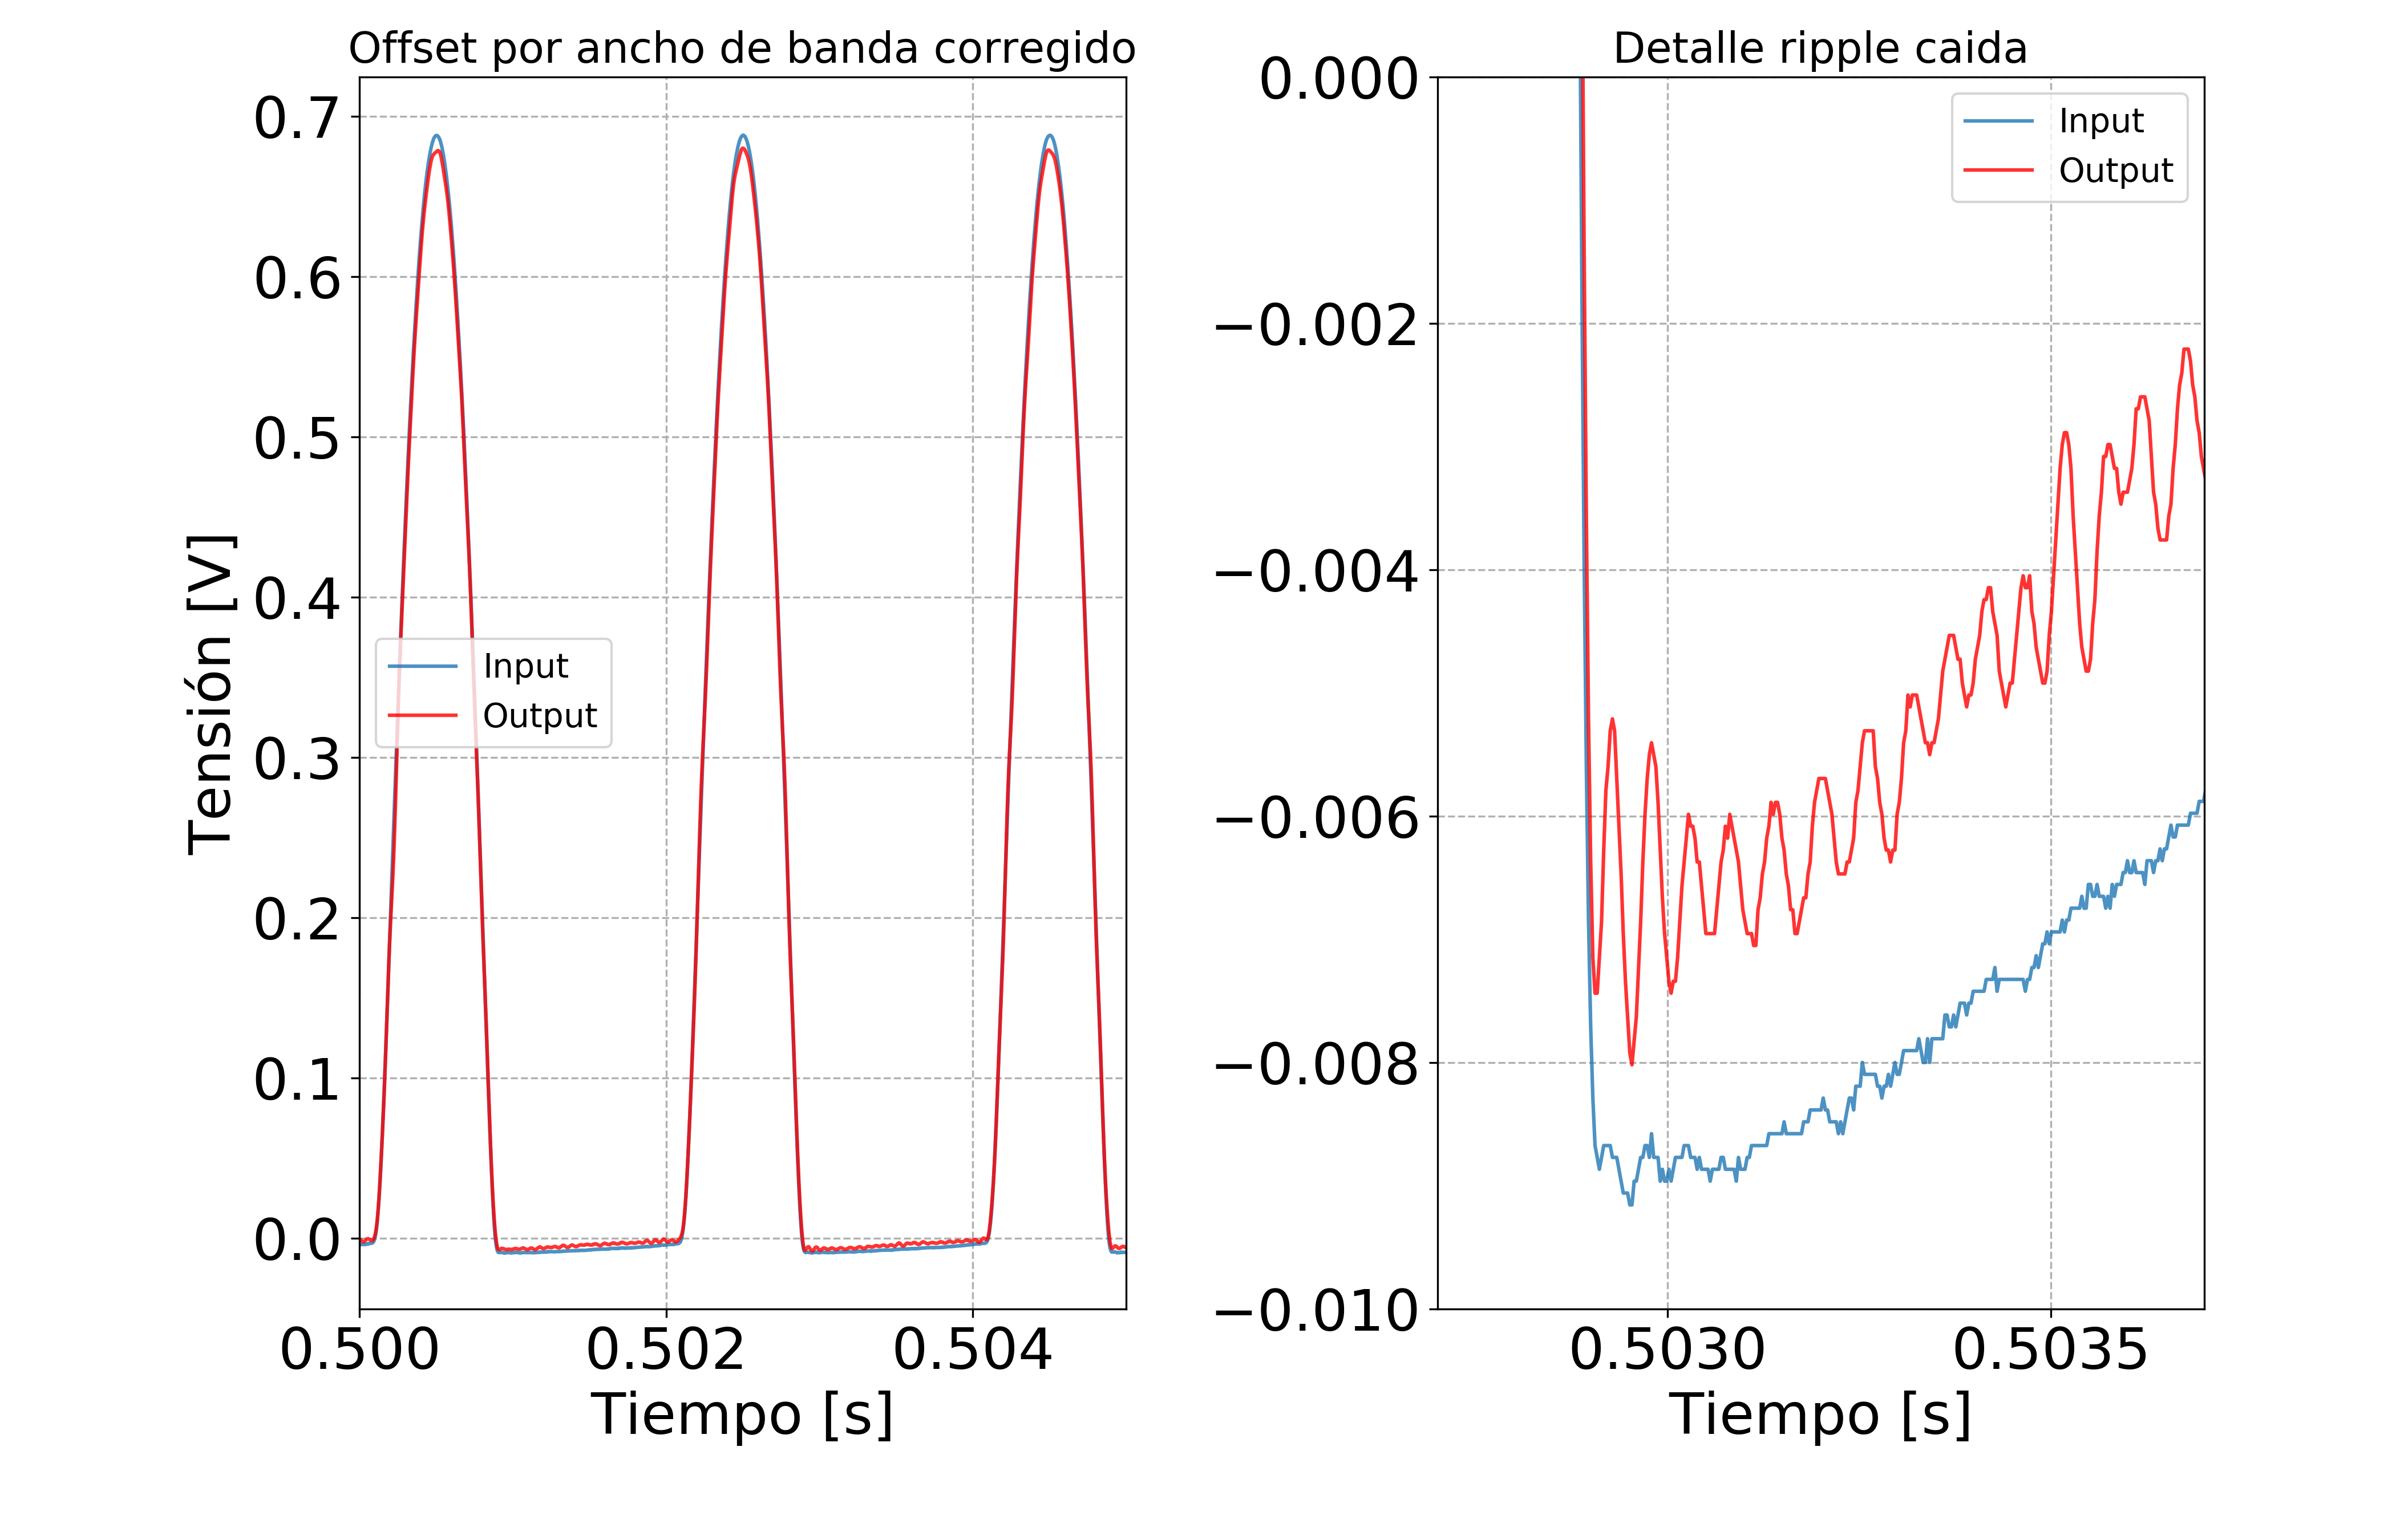
\includegraphics[scale=0.45]{salida_diodo.png}
%\caption{ Seguidor alimentado con -5 V\label{fig:salida_diodo}}
%\end{figure} 
%
%\begin{figure} [H]
%\centering
%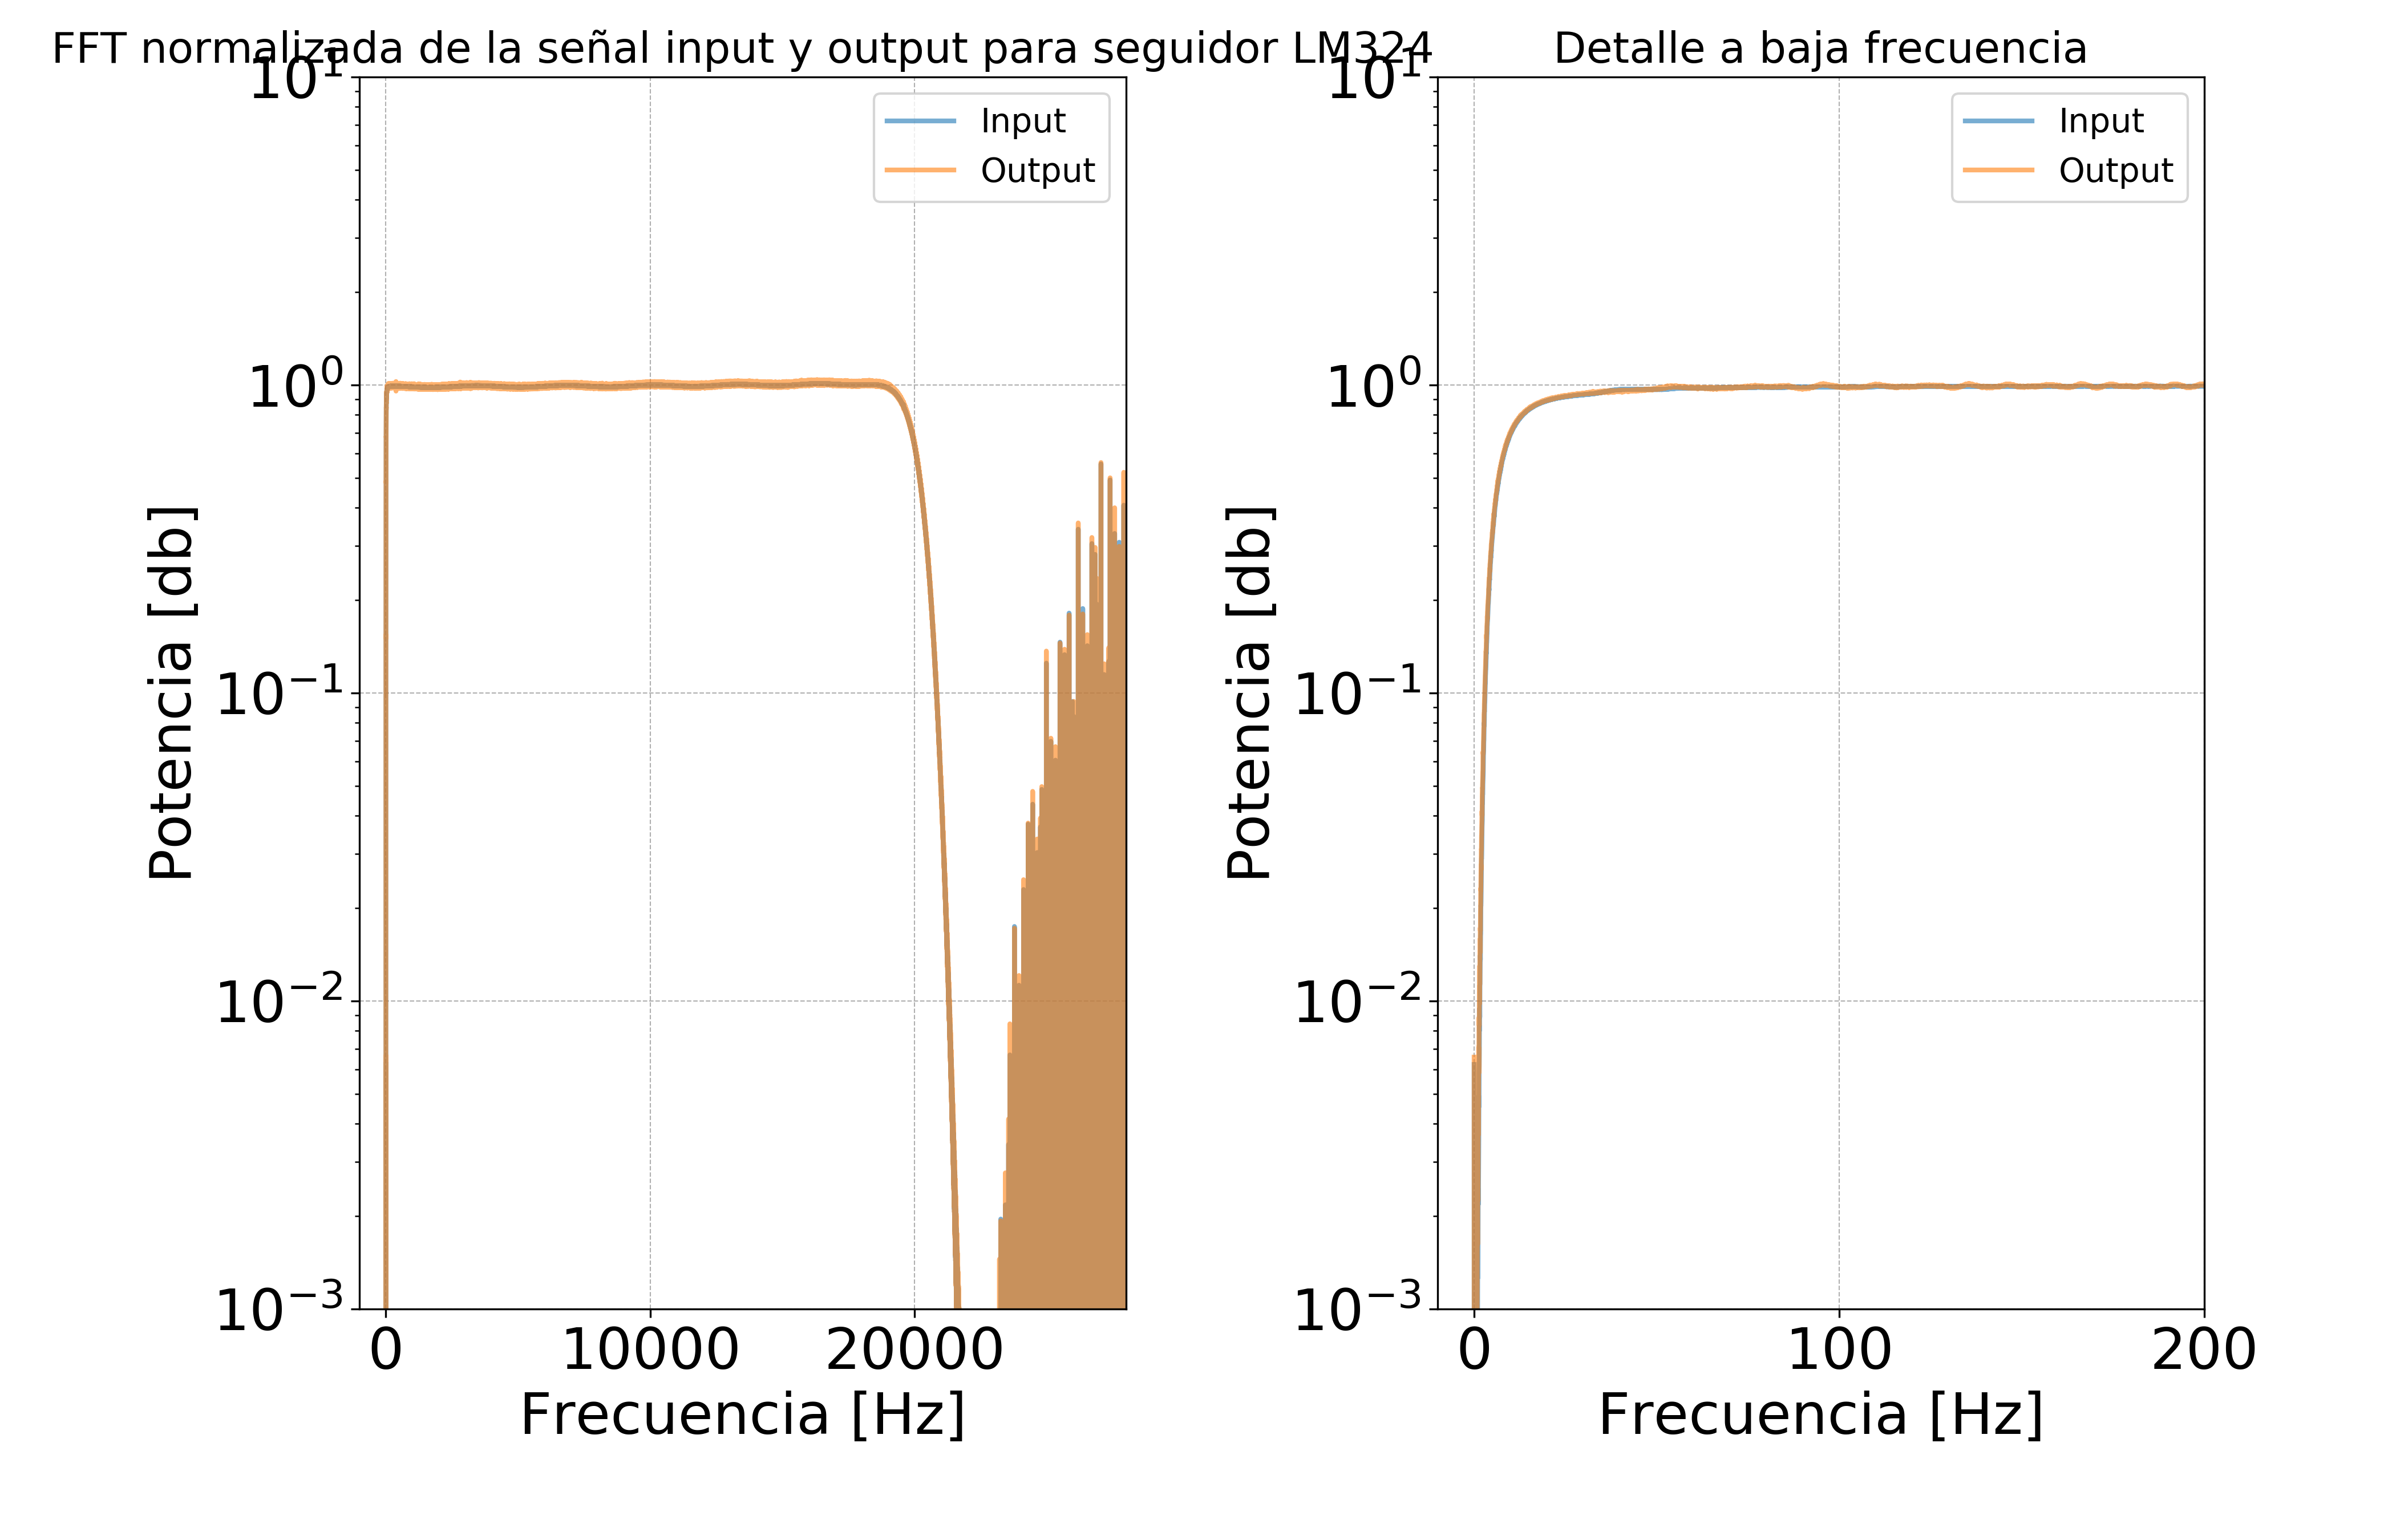
\includegraphics[scale=0.45]{chirp_normalizada.png}
%\caption{ Seguidor alimentado con -5 V\label{fig:chirp_normalizada}}
%\end{figure} 


\subsubsection*{Amplificador}

A continuación realizamos un estudio del amplificador operacional LM324 en modo amplificador no inversor según el esquema de la Figura \ref{fig:amplificador}. El estudio constió en verificar la validez de la curva de ganancia teórica dada por la siguiente relación y estudiar el ancho de banda del op-amp a medida que aumentamos la ganancia del mismo.

\[
 G = 1 + \frac{R2}{R1}
\]


\begin{figure} [H]
\centering
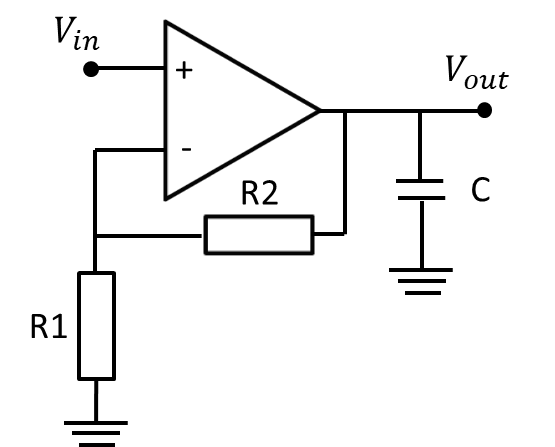
\includegraphics[scale=0.75]{amplificador.png}
\caption{ Esquema amplificador no inversor. \label{fig:amplificador}}
\end{figure} 


En la Figura \ref{fig:salida_amplificador} se muestra la salida del op-amp al enviar una señal sinusoidal de 500 Hz con valores de resistencias de R1 = 4600 Ohms, R2 = 100000 Ohms y C = 22 pF. A la derecha vemos cómo se verifica la linealidad entre la salida y la entrada, en donde la pendiente, que representa la ganancia del circuito, es de 22.33. Si consideramos la ganancia teórica obtenemos un valor de 22.73, por lo que podemos considerar que para estos valores de ganancia estamos dentro del rango de respuesta lineal del circuito.

\begin{figure} [H]
\centering
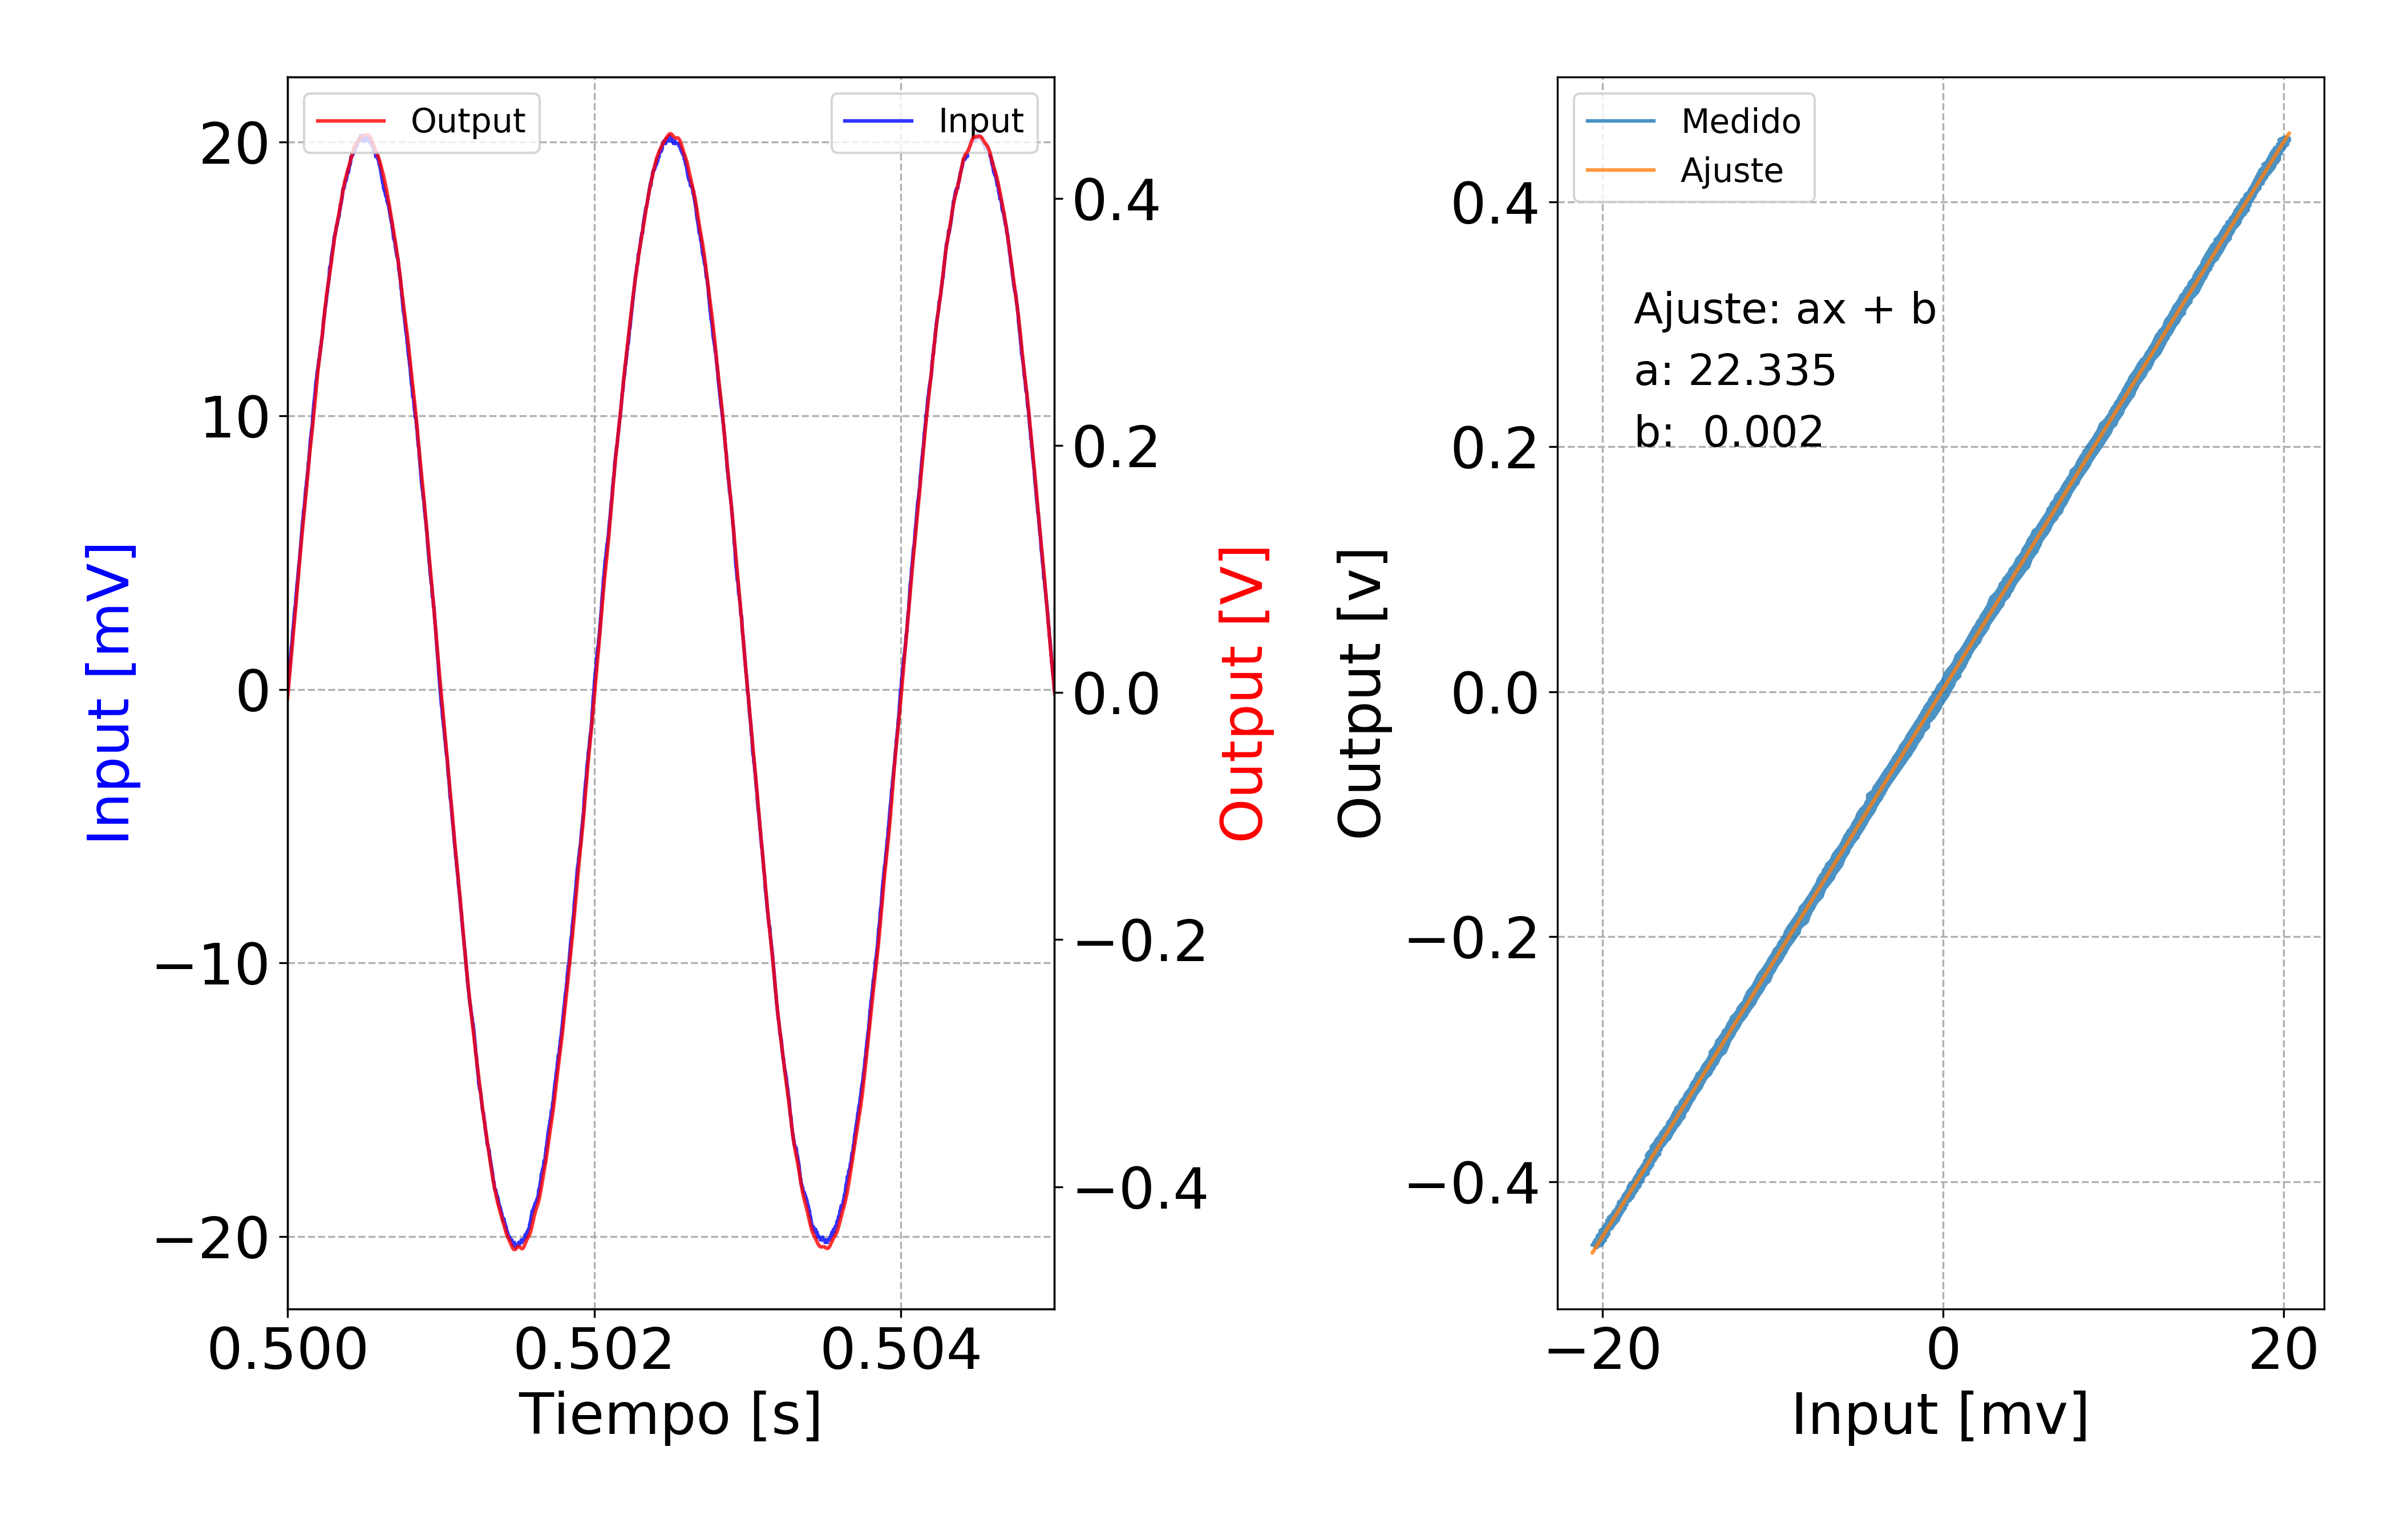
\includegraphics[scale=0.45]{salida_amplificador.png}
\caption{ Amplificador\label{fig:salida_amplificador}}
\end{figure} 

A continuación nos proponemos estudiar el comportamiento del circuito para distintos valores de ganancias y para distintas frecuencias de entrada. Para ello fuimos variando la resistencia R1 (R2 fijo en 100 KOhms y C de 22 pF), y medimos la entrada y salida del opamp al enviar un seno con chirp. De esta manera la obtención de la ganancia para cada frecuencia es simplemente la relación entre la respuesta espectral del chirp a la entrada y salida del circuito. Teniendo en cuenta la limitación en el rango de tensión de entrada de la placa de audio, se eligieron amplitudes de entrada al opamp lo suficientemente bajas para no saturar la placa con la salida del opamp. En la Figura \ref{fig:respuestas_r1} mostramos la respuesta en frecuencias del amplificador a medida que variamos la relación R2/R1 del circuito (o sea a medida que aumentamos la ganancia del circuito). En este caso normalizamos las curvas a la respuesta teórica del chirp (al igual que lo hicimos anteriormente) y también al valor de respuesta obtenido a 1000 Hz. Es decir que el gráfico no permite verificar el aumento de la ganancia al variar la relación R1/R2, pero permite ver cómo se reduce su ancho de banda. 

\begin{figure} [H]
\centering
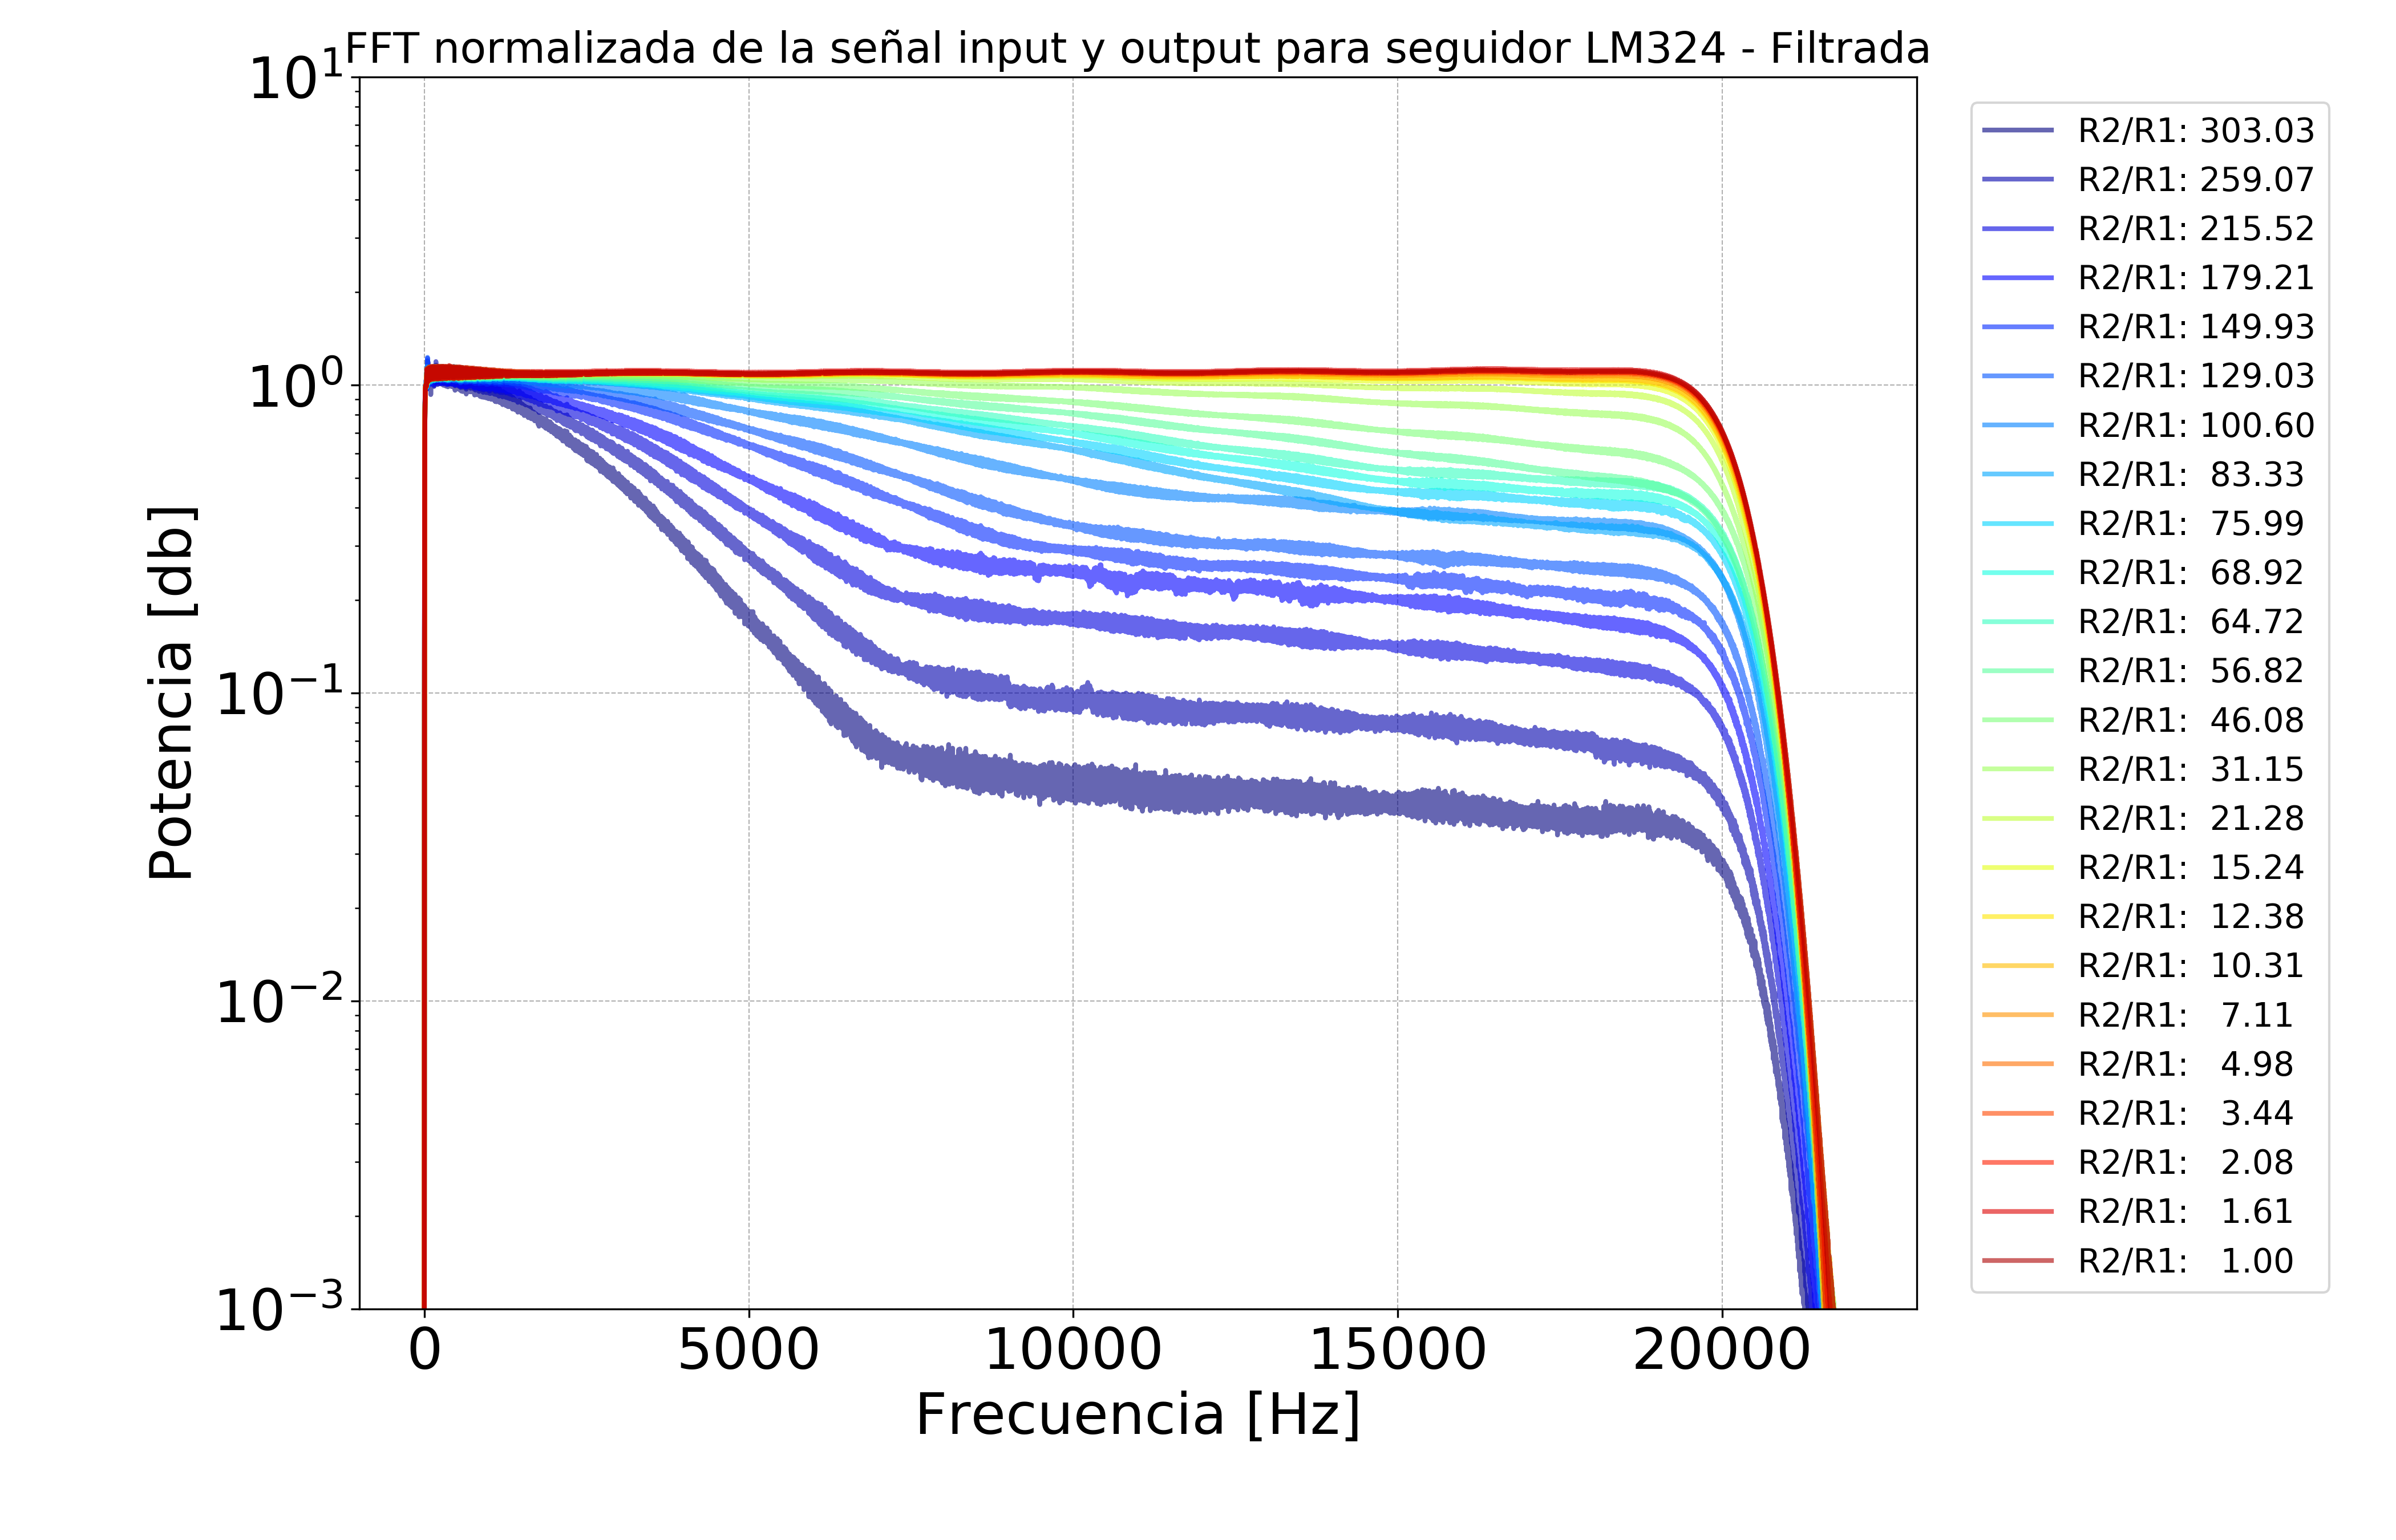
\includegraphics[scale=0.45]{respuestas_r1.png}
\caption{ Respuesta en frecuencias del amplificador al variar la relación R2/R1. \label{fig:respuestas_r1}}
\end{figure} 

Para estudiar la ganancia consideramos el gráfico de la Figura \ref{fig:ganancia_ancho_de_banda} donde mostramos la ganancia del circuito para distintos valores de R2/R1 y a distintas frecuencias. Como se dijo anteriormente la ganancia se obtuvo a partir de hacer la relación de la respuesta espectral de la entrada y la salida, luego de realizar la calibración en tensión de ambos canales. Cabe destacar que en este caso realizamos el cociente en amplitud entre la curvas, a diferencia del caso anterior en donde se consideraba la potencia. Como se puede observar del gráfico vemos que la respuesta lineal de la ganancia con la relación R2/R1 se verifica para ganancias pequeñas o para frecuencias bajas (o sea cuando la ganancia no está afectada por la disminución del ancho de banda). En particular, al realizar el ajuste lineal para el caso de 200 Hz obtenemos una pendiente de 1.002 y ordenada al origen de 0.25, siendo ambos valores esperados iguales 1 (tener en cuenta la fórmula de ganancia mostarada arriba). A la derecha graficamos el ancho de banda en función de R2/R1, obtenido a partir de medir la frecuencia para la cual la potencia cae a la mitad. En el gráfico mostramos la restricción en el ancho de banda debido a la limitación de la placa de video.

\begin{figure} [H]
\centering
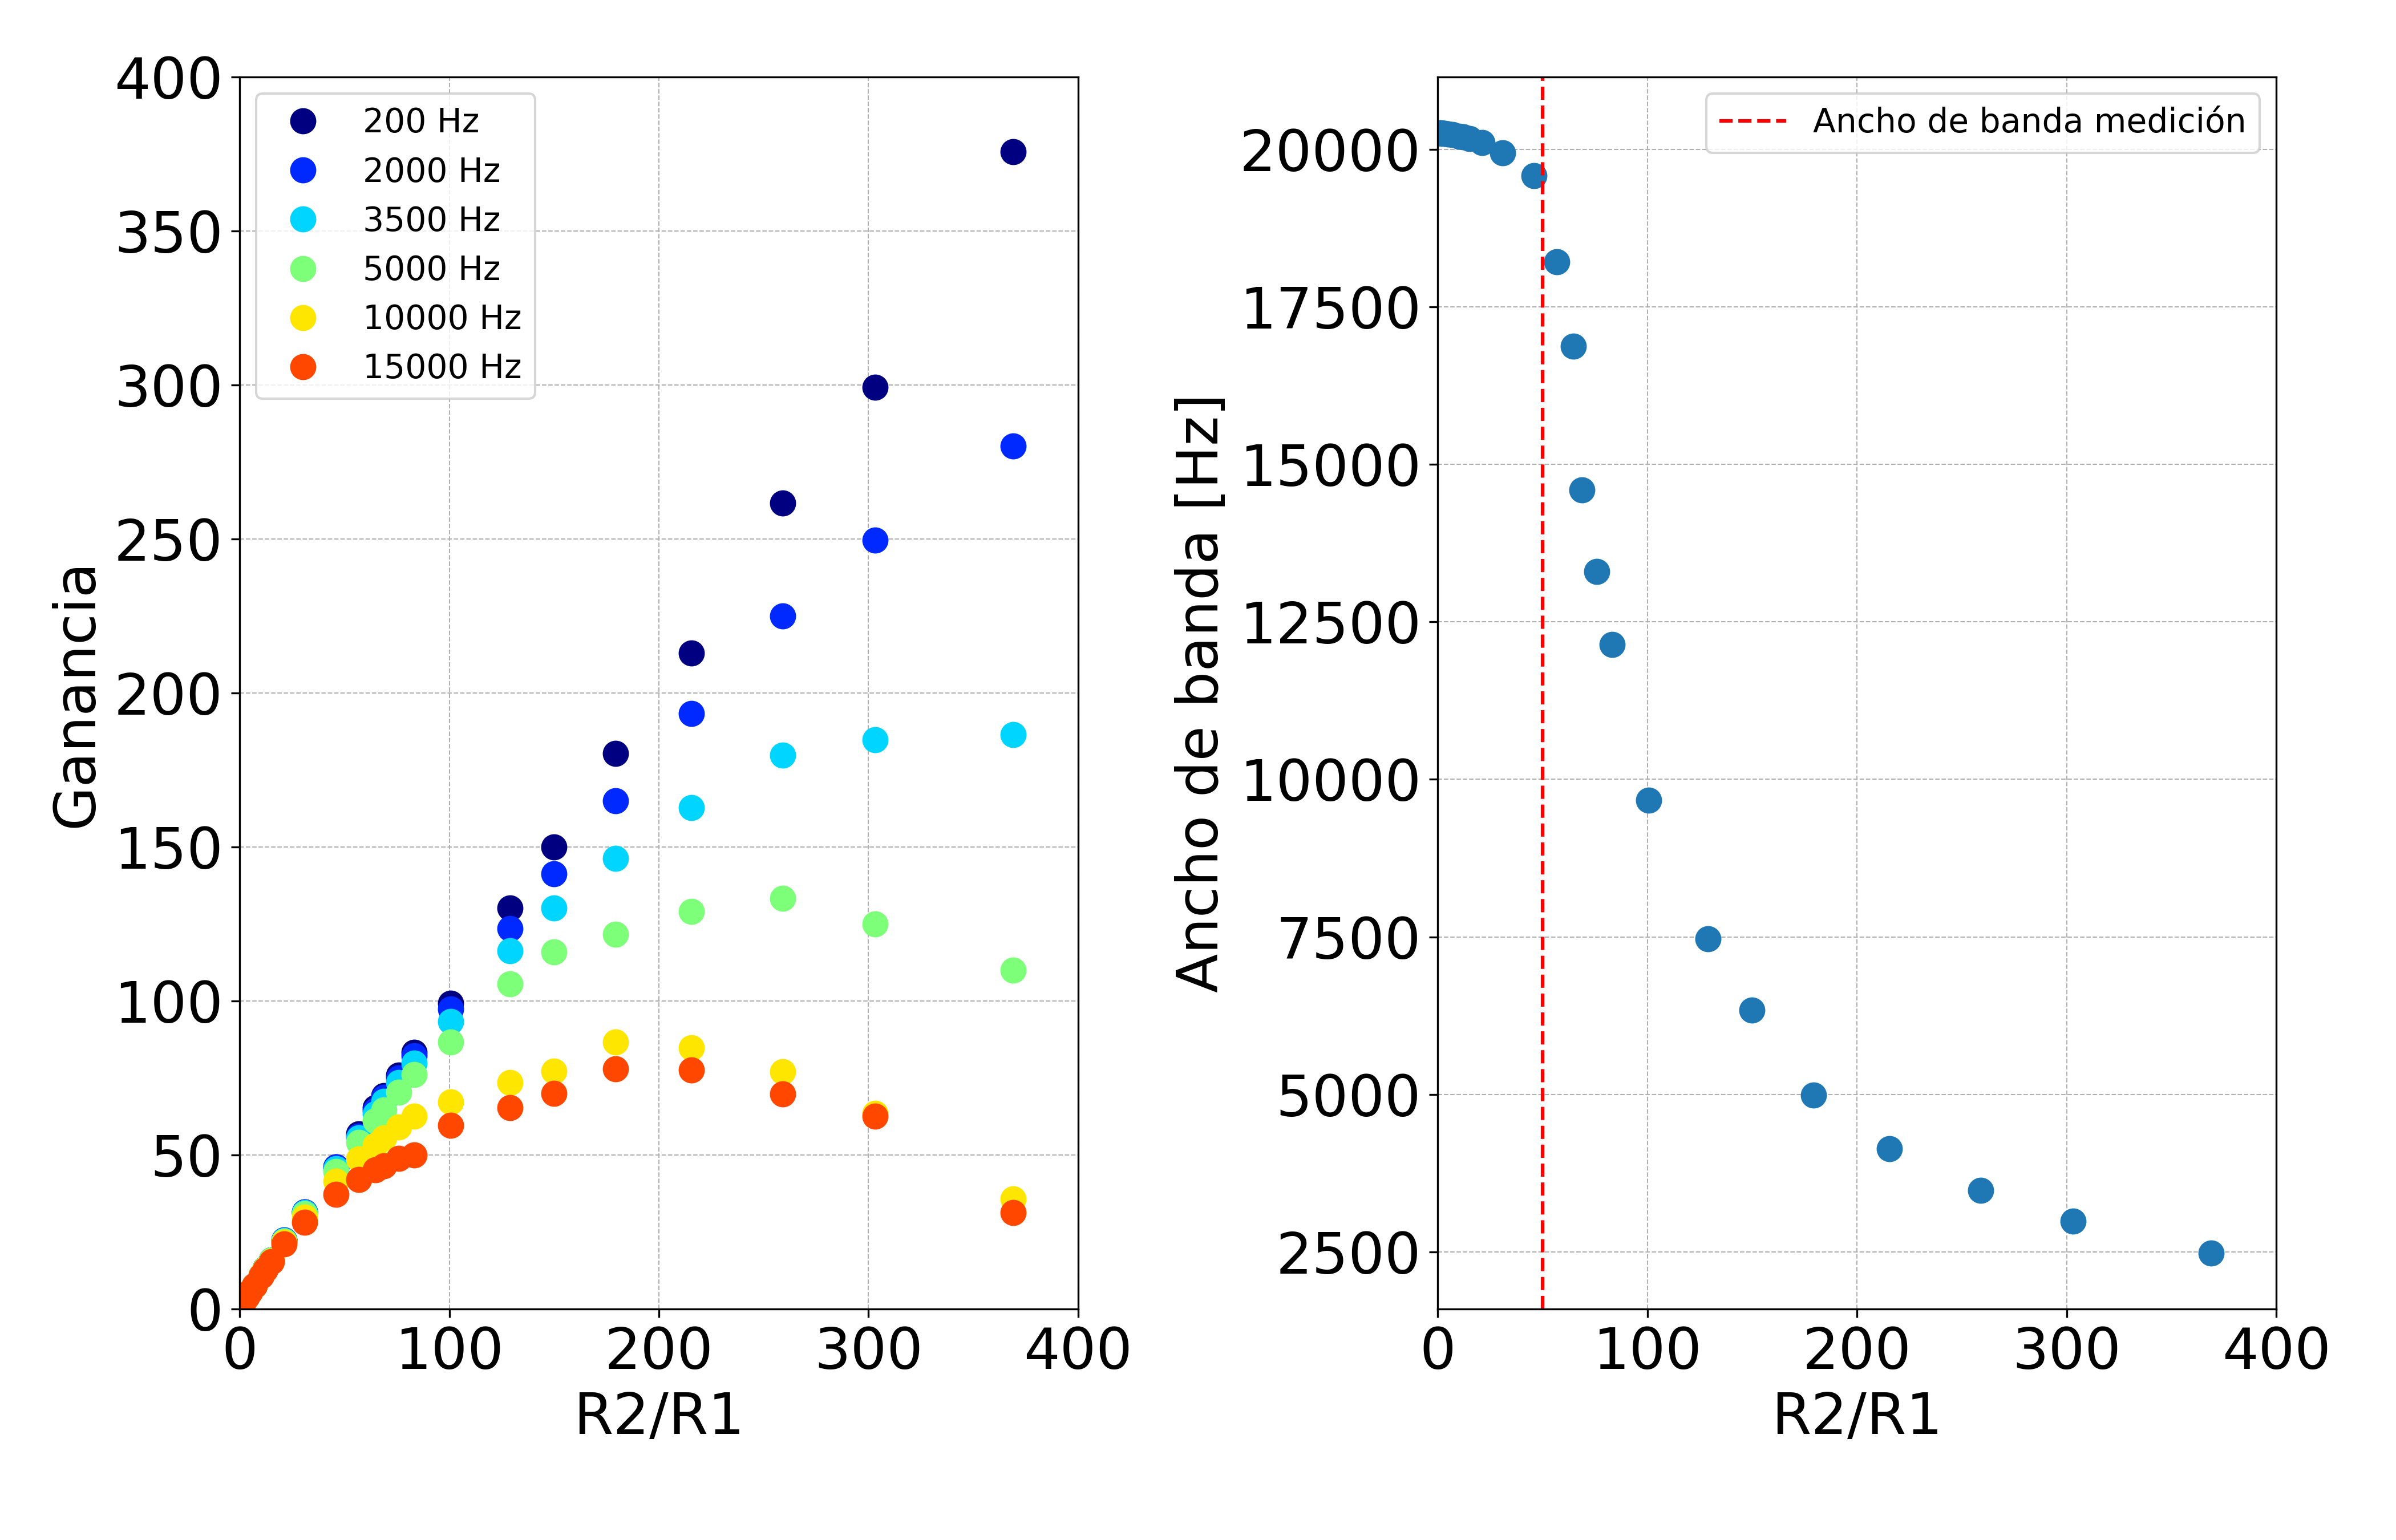
\includegraphics[scale=0.45]{ganancia_ancho_de_banda.png}
\caption{ Izquierda: Ganancia del amplificador en función de R2/R1. Observese que la linealidad de la ganancia con R2/R1 es válida para ganacias bajas o frecuencias de señal bajas. Derecha: ancho de banda en fucnión de R2/R1 obtenido a partir de las curvas del gráfico de la Figura anterior. \label{fig:ganancia_ancho_de_banda}}
\end{figure} 

A continuación (Figura\ref{fig:ganancia_ancho_de_banda_1} ) graficamos la ganancia en función del ancho de banda obtenida a partir de combinar los graficos de la Figura anterior. También mostramos el producto entre la ganancia y el ancho de banda en función de la ganancia para una señal de 200 Hz, que es constante en el op-amp ideal (!! Referencia!!).

\begin{figure} [H]
\centering
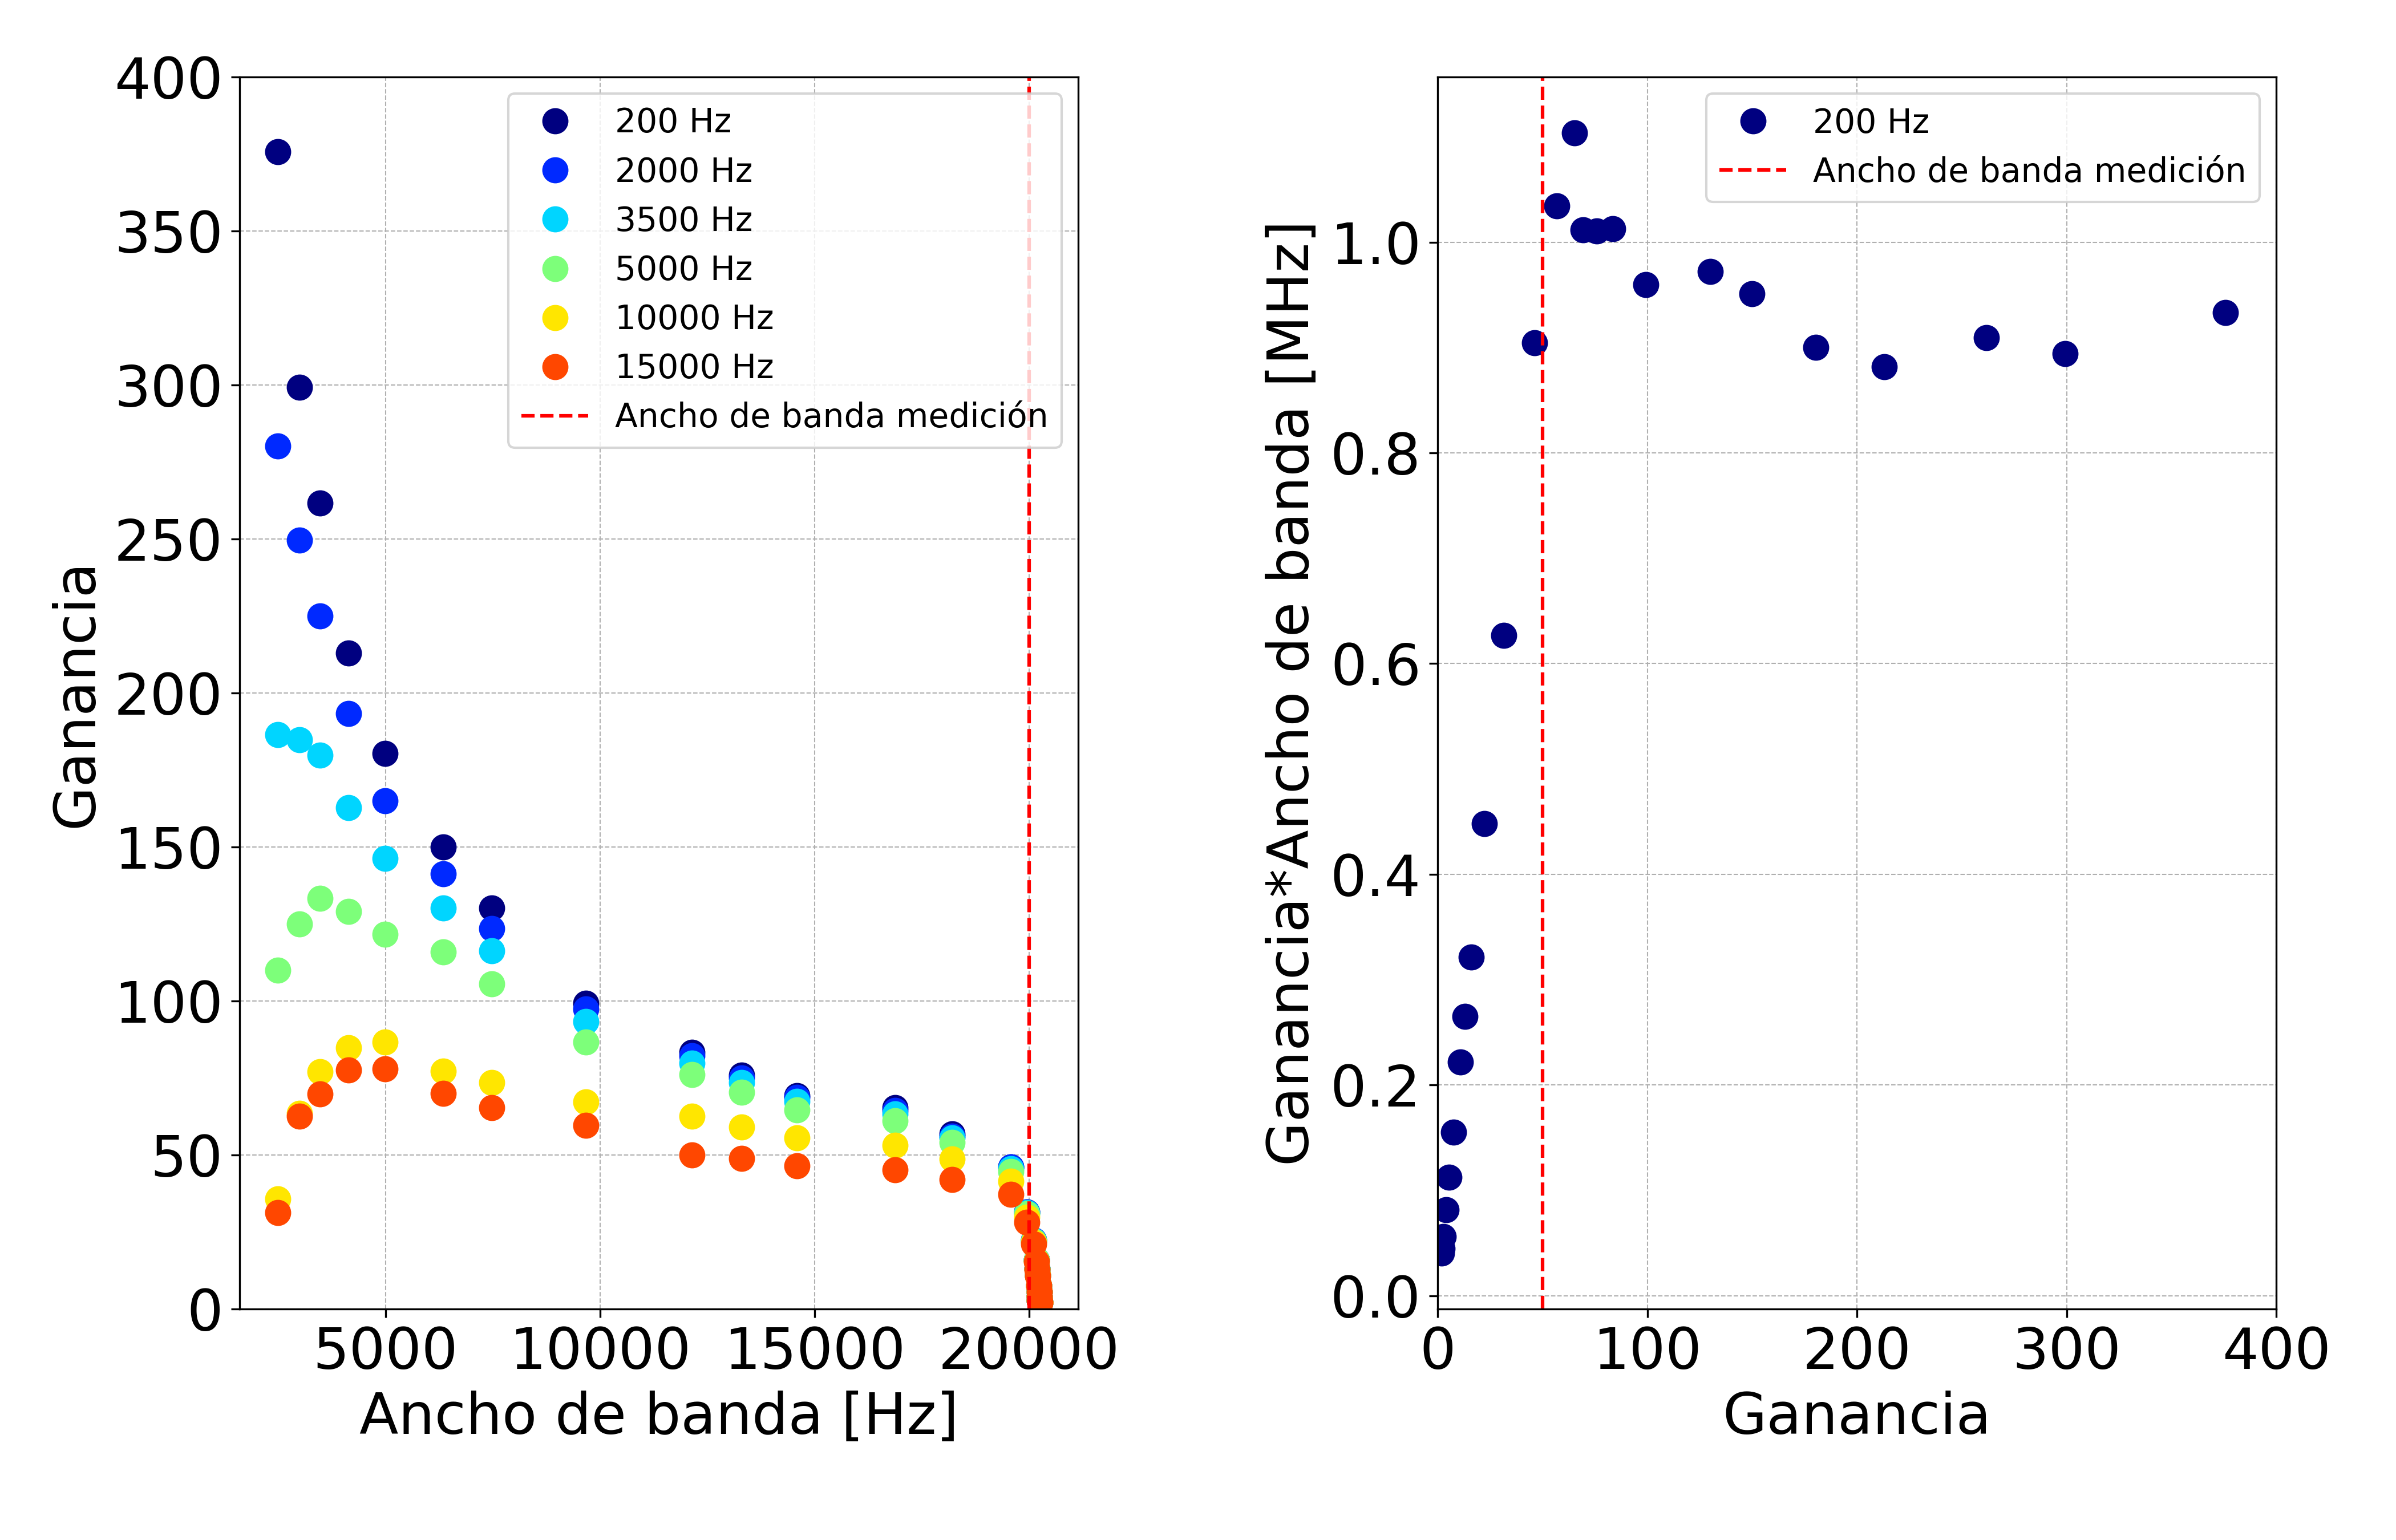
\includegraphics[scale=0.45]{ganancia_ancho_de_banda_1.png}
\caption{ Izquierda: Ganancia en función del ancho de banda a distintas frecuencias de señal. Derecha: producto entre la ganancia y el ancho de banda en función de la ganancia para señal de 200 Hz. \label{fig:ganancia_ancho_de_banda_1}}
\end{figure} 


%El objetivo es medir la ganancia para dsitintas frecuencias. 
%\subsubsection*{frecuencia de corte}
%La idea aquí es armar un amplificador inversor y medir la frecuencia de corte para distintas ganancias. Para esto hay que tener en cuenta el rango de tensión que podemos medir con la placa, es decir variar las resistencias del amplificador para que la ganancia no sea tal que la señal sature
%
%\subsubsection*{Figure Noise}
%
%\subsubsection*{Slew Rate}

\section*{Anexo:}
\subsection*{Programa de adquisición}
El programa de adquisición permite la utilización de la placa de audio de la pc como un generador de funciones (parlante) de dos canales y un osciloscopio de dos canales, utilizando la librería pyaudio. La función encargada de la adquisición (\textit{playrec}) acepta una matriz de tres dimensiones donde se guarda la señal que se quiere enviar en cada canal de salida. La primera dimensión es la cantidad de pasos del barrido que se quiere realizar. La segunda es la cantidad de muestras enviadas y depende de la duración de la señal enviada y la frecuencia de sampleo según la relación $muestras=frec_{sampleo}*duracion_{signal}$. La tercera dimensión indica el canal de salida (CH0 y CH1).
Una vez que se recibe la matriz, se definen los buffer de salida y de entrada. El buffer de salida tiene el tamaño en bytes equivalente a cada fila del barrido. El buffer de entrada es siempre más grande, pues se contempla la adquisición de ceros al principio de la medición debido al retardo entre la señal enviada y la señal adquirida. Además se obliga a que el número de muestras del buffer de entrada sea múltiplo de una potencia de 2.
Una vez definido los buffers se lanzan dos hilos de procesamiento encargados de la escritura de los datos en el buffer de salida (hilo productor) y la lectura de los datos del buffer de entrada (hilo consumidor). La comunicación entre los dos hilos se realiza con dos variables de tipo lock. La primera se activa cada vez que el productor escribe la señal en el buffer de salida y avisa al consumidor que puede empezar la adquisición. El segundo lock se activa en el consumidor cada vez que se termina de leer el buffer de entrada y se guardó la señal en la matriz de salida, y avisa al productor que puede comenzar el envío del siguiente paso del barrido.
Por último se agrega la posibilidad de corregir el retardo de la medición a partir de encontrar el máximo de la correlación cruzada entre la señal digital enviada y la señal adquirida.

\begin{figure} [H]
\centering
\includegraphics[scale=0.85]{esquema_adquisicion.png}
\caption{Esquema de adquisición. \label{fig:esquema_adquisiciona}}
\end{figure} 


\subsection*{Ejemplo}
La señal de salida digital es de tipo float32 y debe ser menor al valor 1 (uno). Los valores mayores a 1 espejan la señal alrededor del éste valor. En la Figura \ref{fig:senal_sintetica} se muestra un ejemplo de señal enviada en los canales CH0 y CH1. 

\begin{figure} [H]
\centering
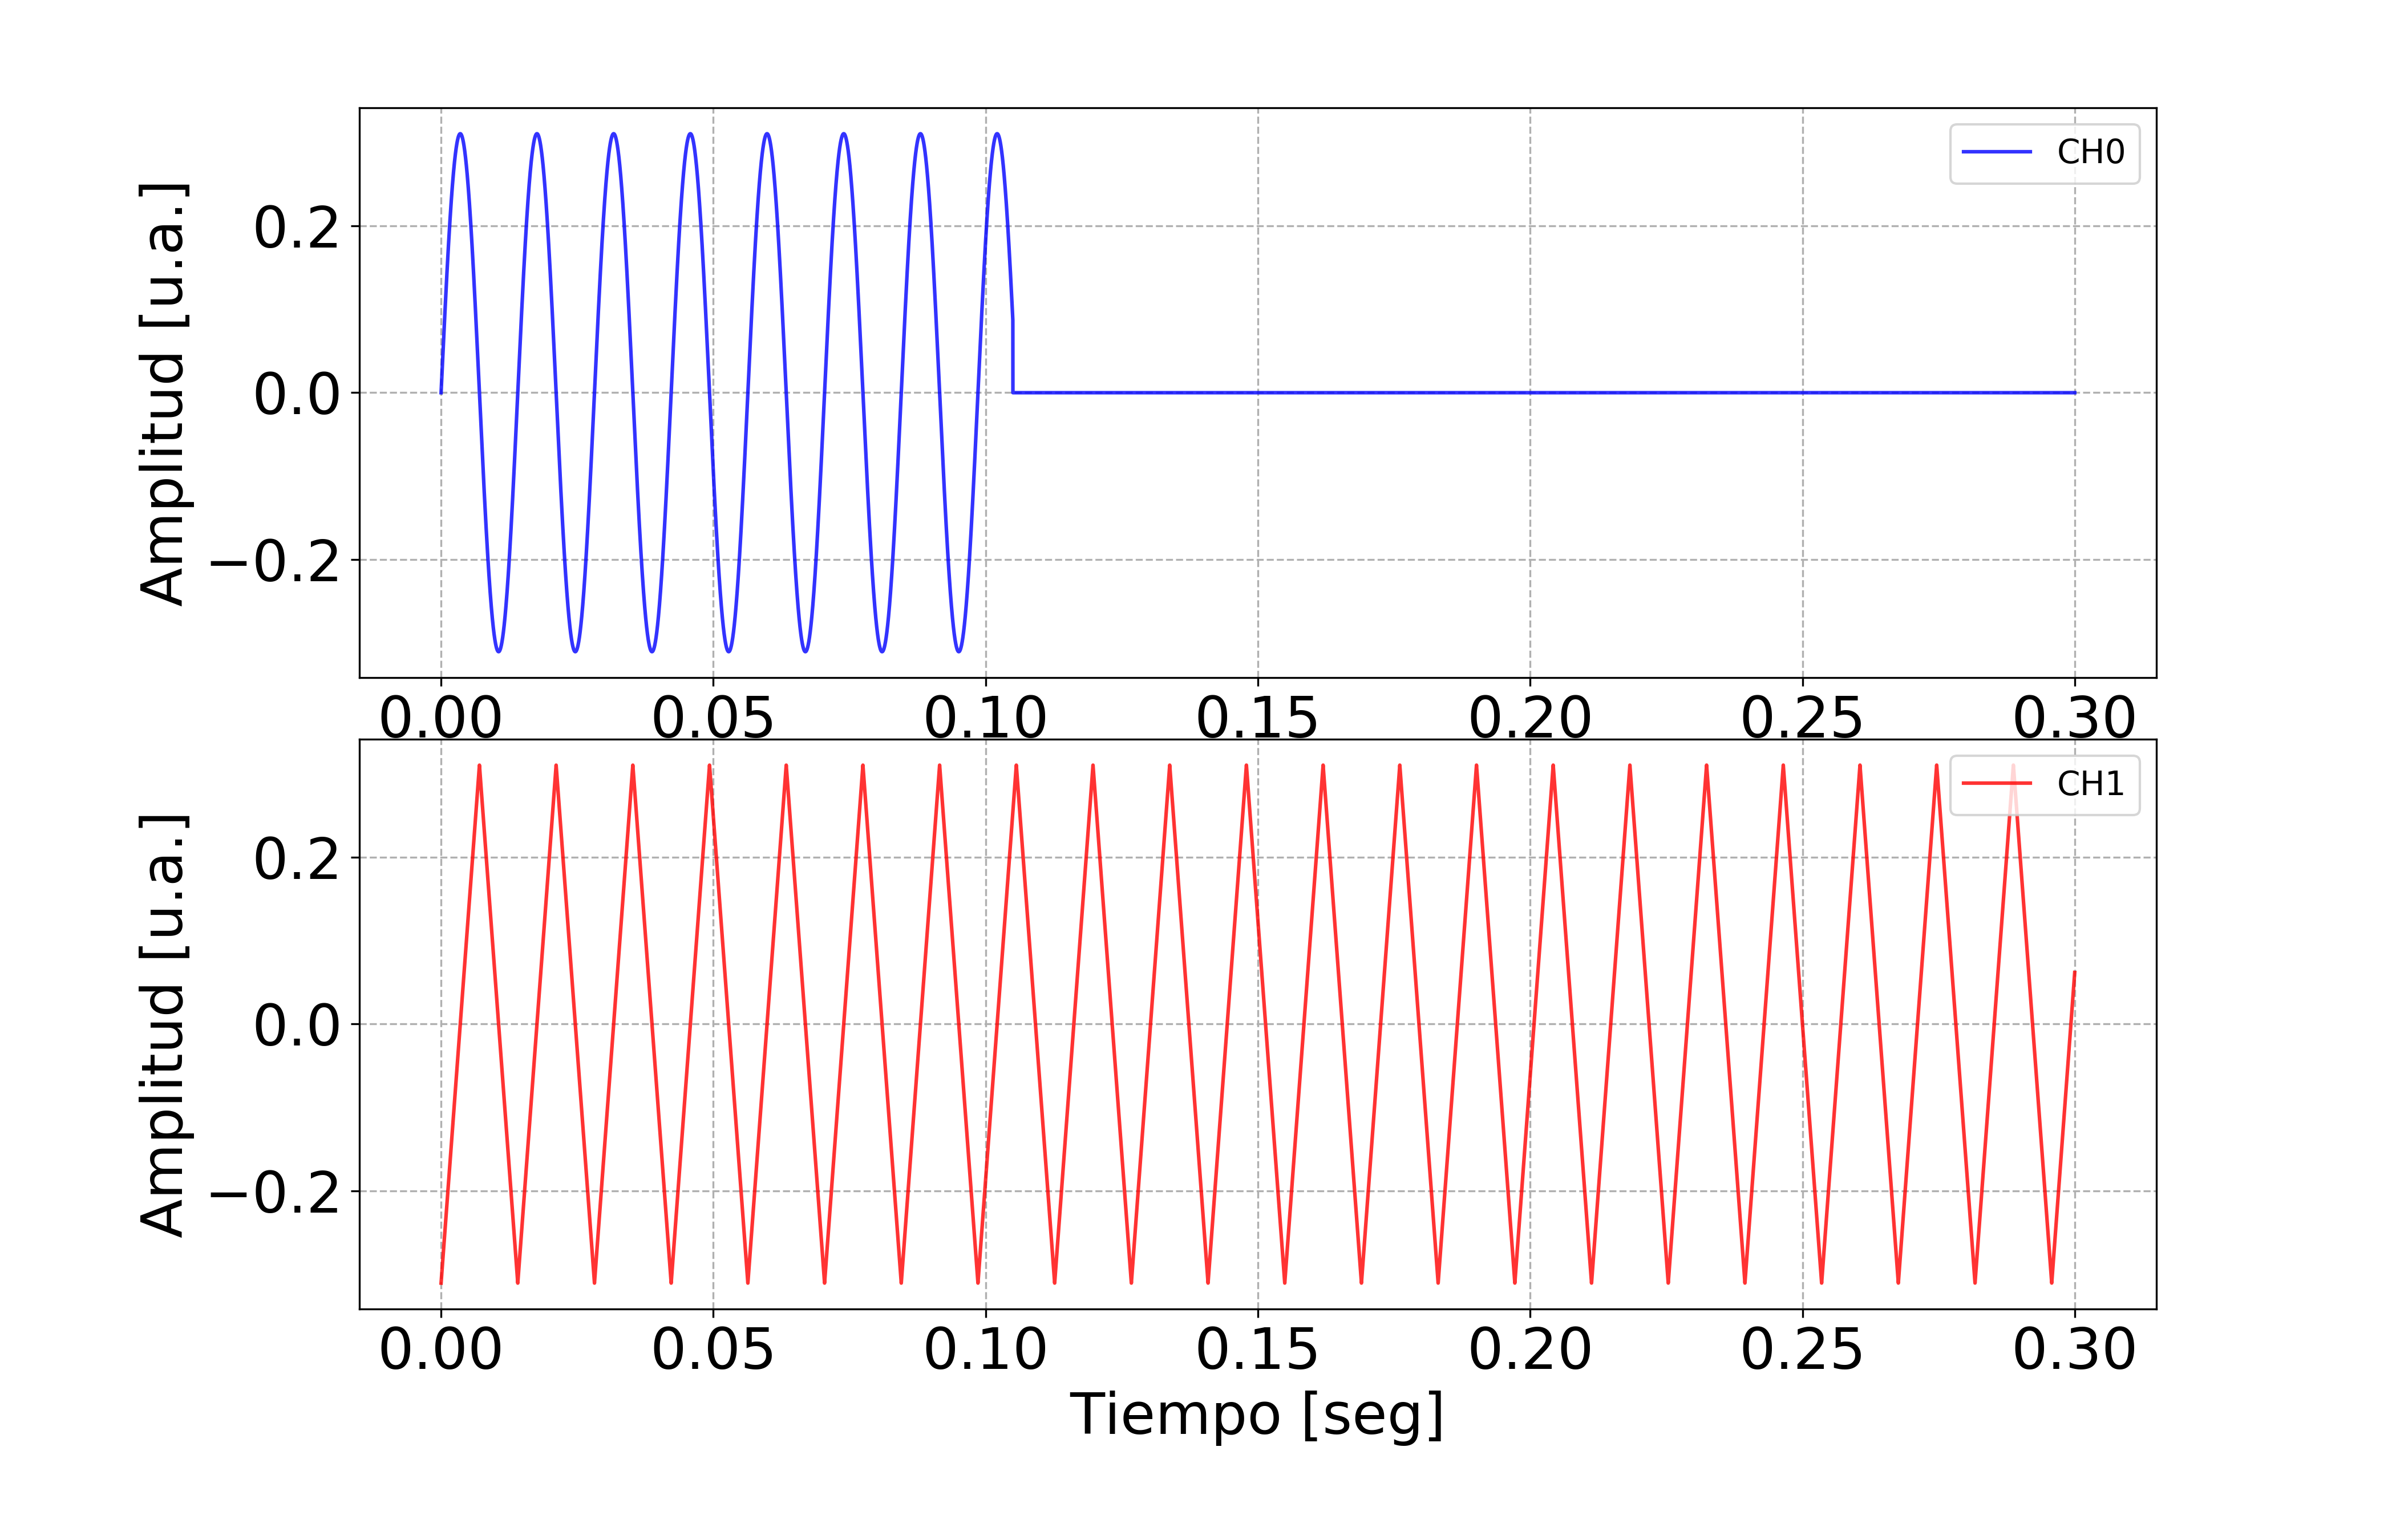
\includegraphics[scale=0.45]{senal_sintetica.png}
\caption{Señal sintética enviada a los canales CH0 y CH1. \label{fig:senal_sintetica}}
\end{figure} 

En la Figura \ref{fig:senal_adquirida} se muestra la señal adquirida antes de realizar la corrección del retardo. Como se puede ver la señal de adquisición es de mayor duración debido a que el buffer de entrada es siempre mayor al de entrada para aseguraros de adquirir toda la señal debido al retardo.


\begin{figure} [H]
\centering
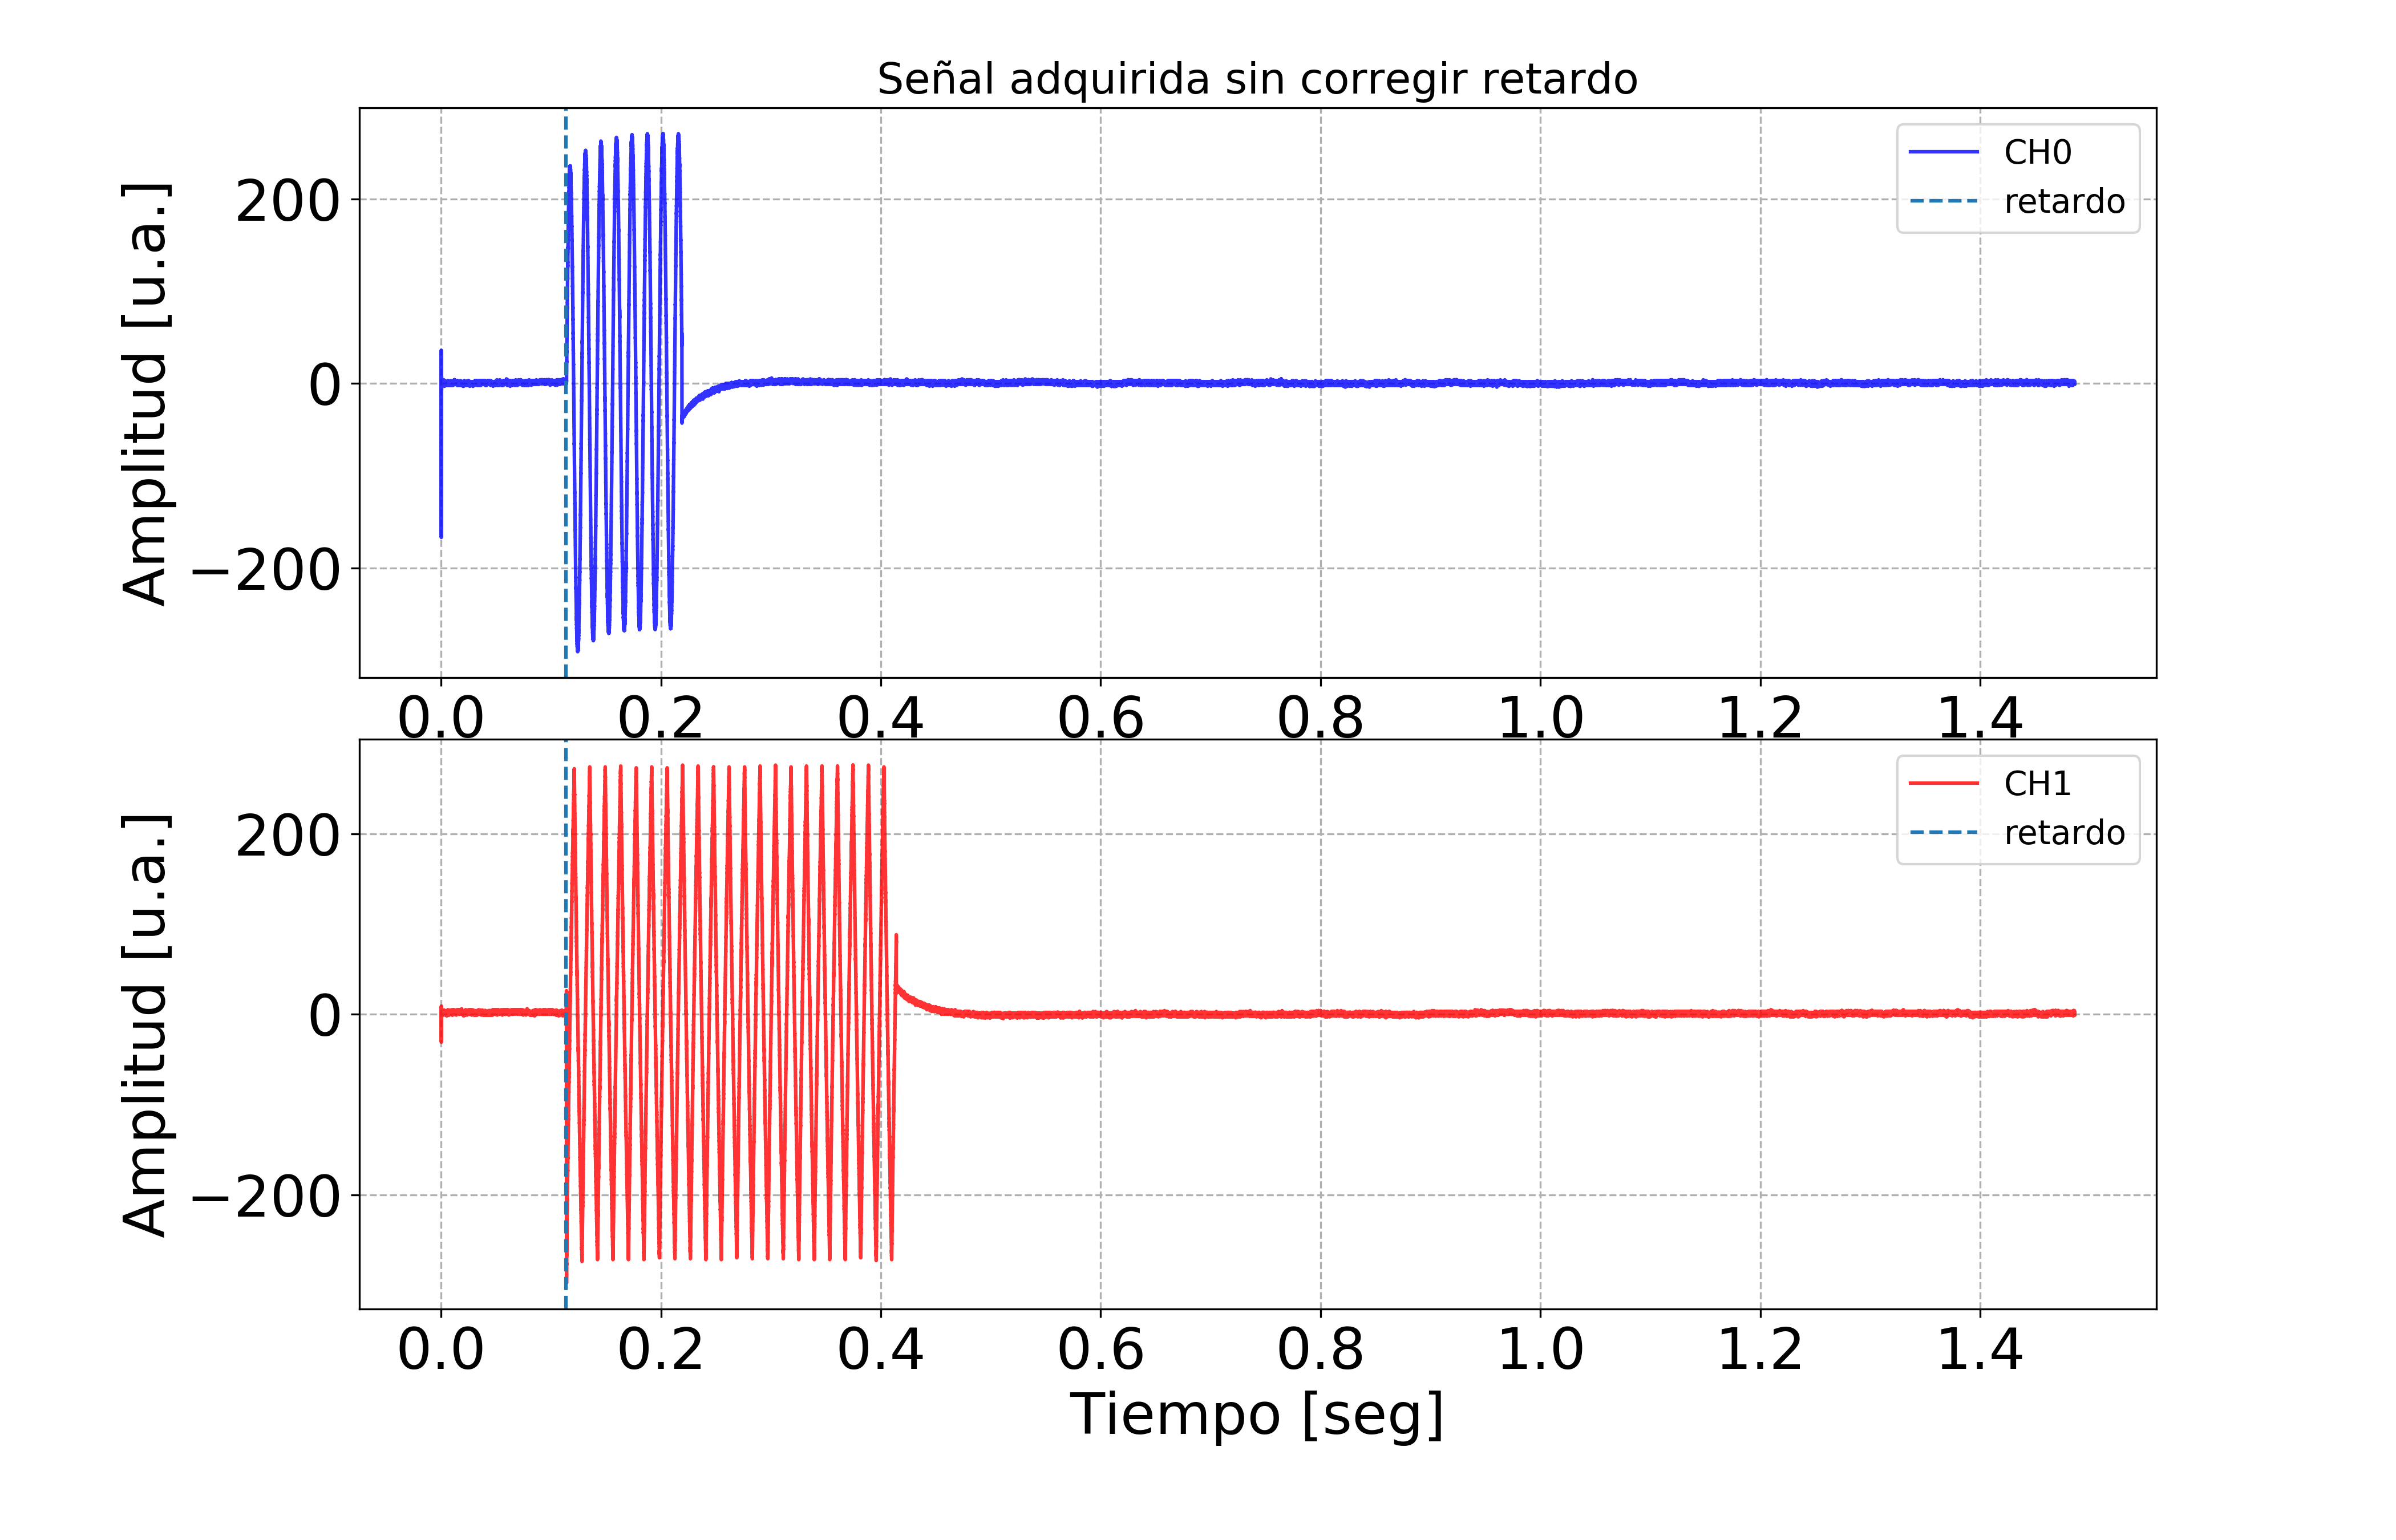
\includegraphics[scale=0.45]{senal_adquirida.png}
\caption{Señal adquirida en los canales CH0 y CH1. \label{fig:senal_adquirida}}
\end{figure} 

En la Figura \ref{fig:correlacion_cruzada} se muestra la correlación cruzada entra la señal digital del canal CH0 y la señal adquirida en el canal CH0. El tiempo transcurrido entre la mitad del vector de correlación y su máximo corresponde al retardo entre las señales. Cabe destacar que la correlación cruzada se realizó en primer lugar con la función correlate de la librería numpy, pero luego se utilizó la función de correlación basada en la FFT propuesta por Lex Fridman (https://lexfridman.com/fast-cross-correlation-and-time-series-synchronization-in-python/). La velocidad de este algoritmo es de hasta 500 veces mejor. 
 
\begin{figure} [H]
\centering
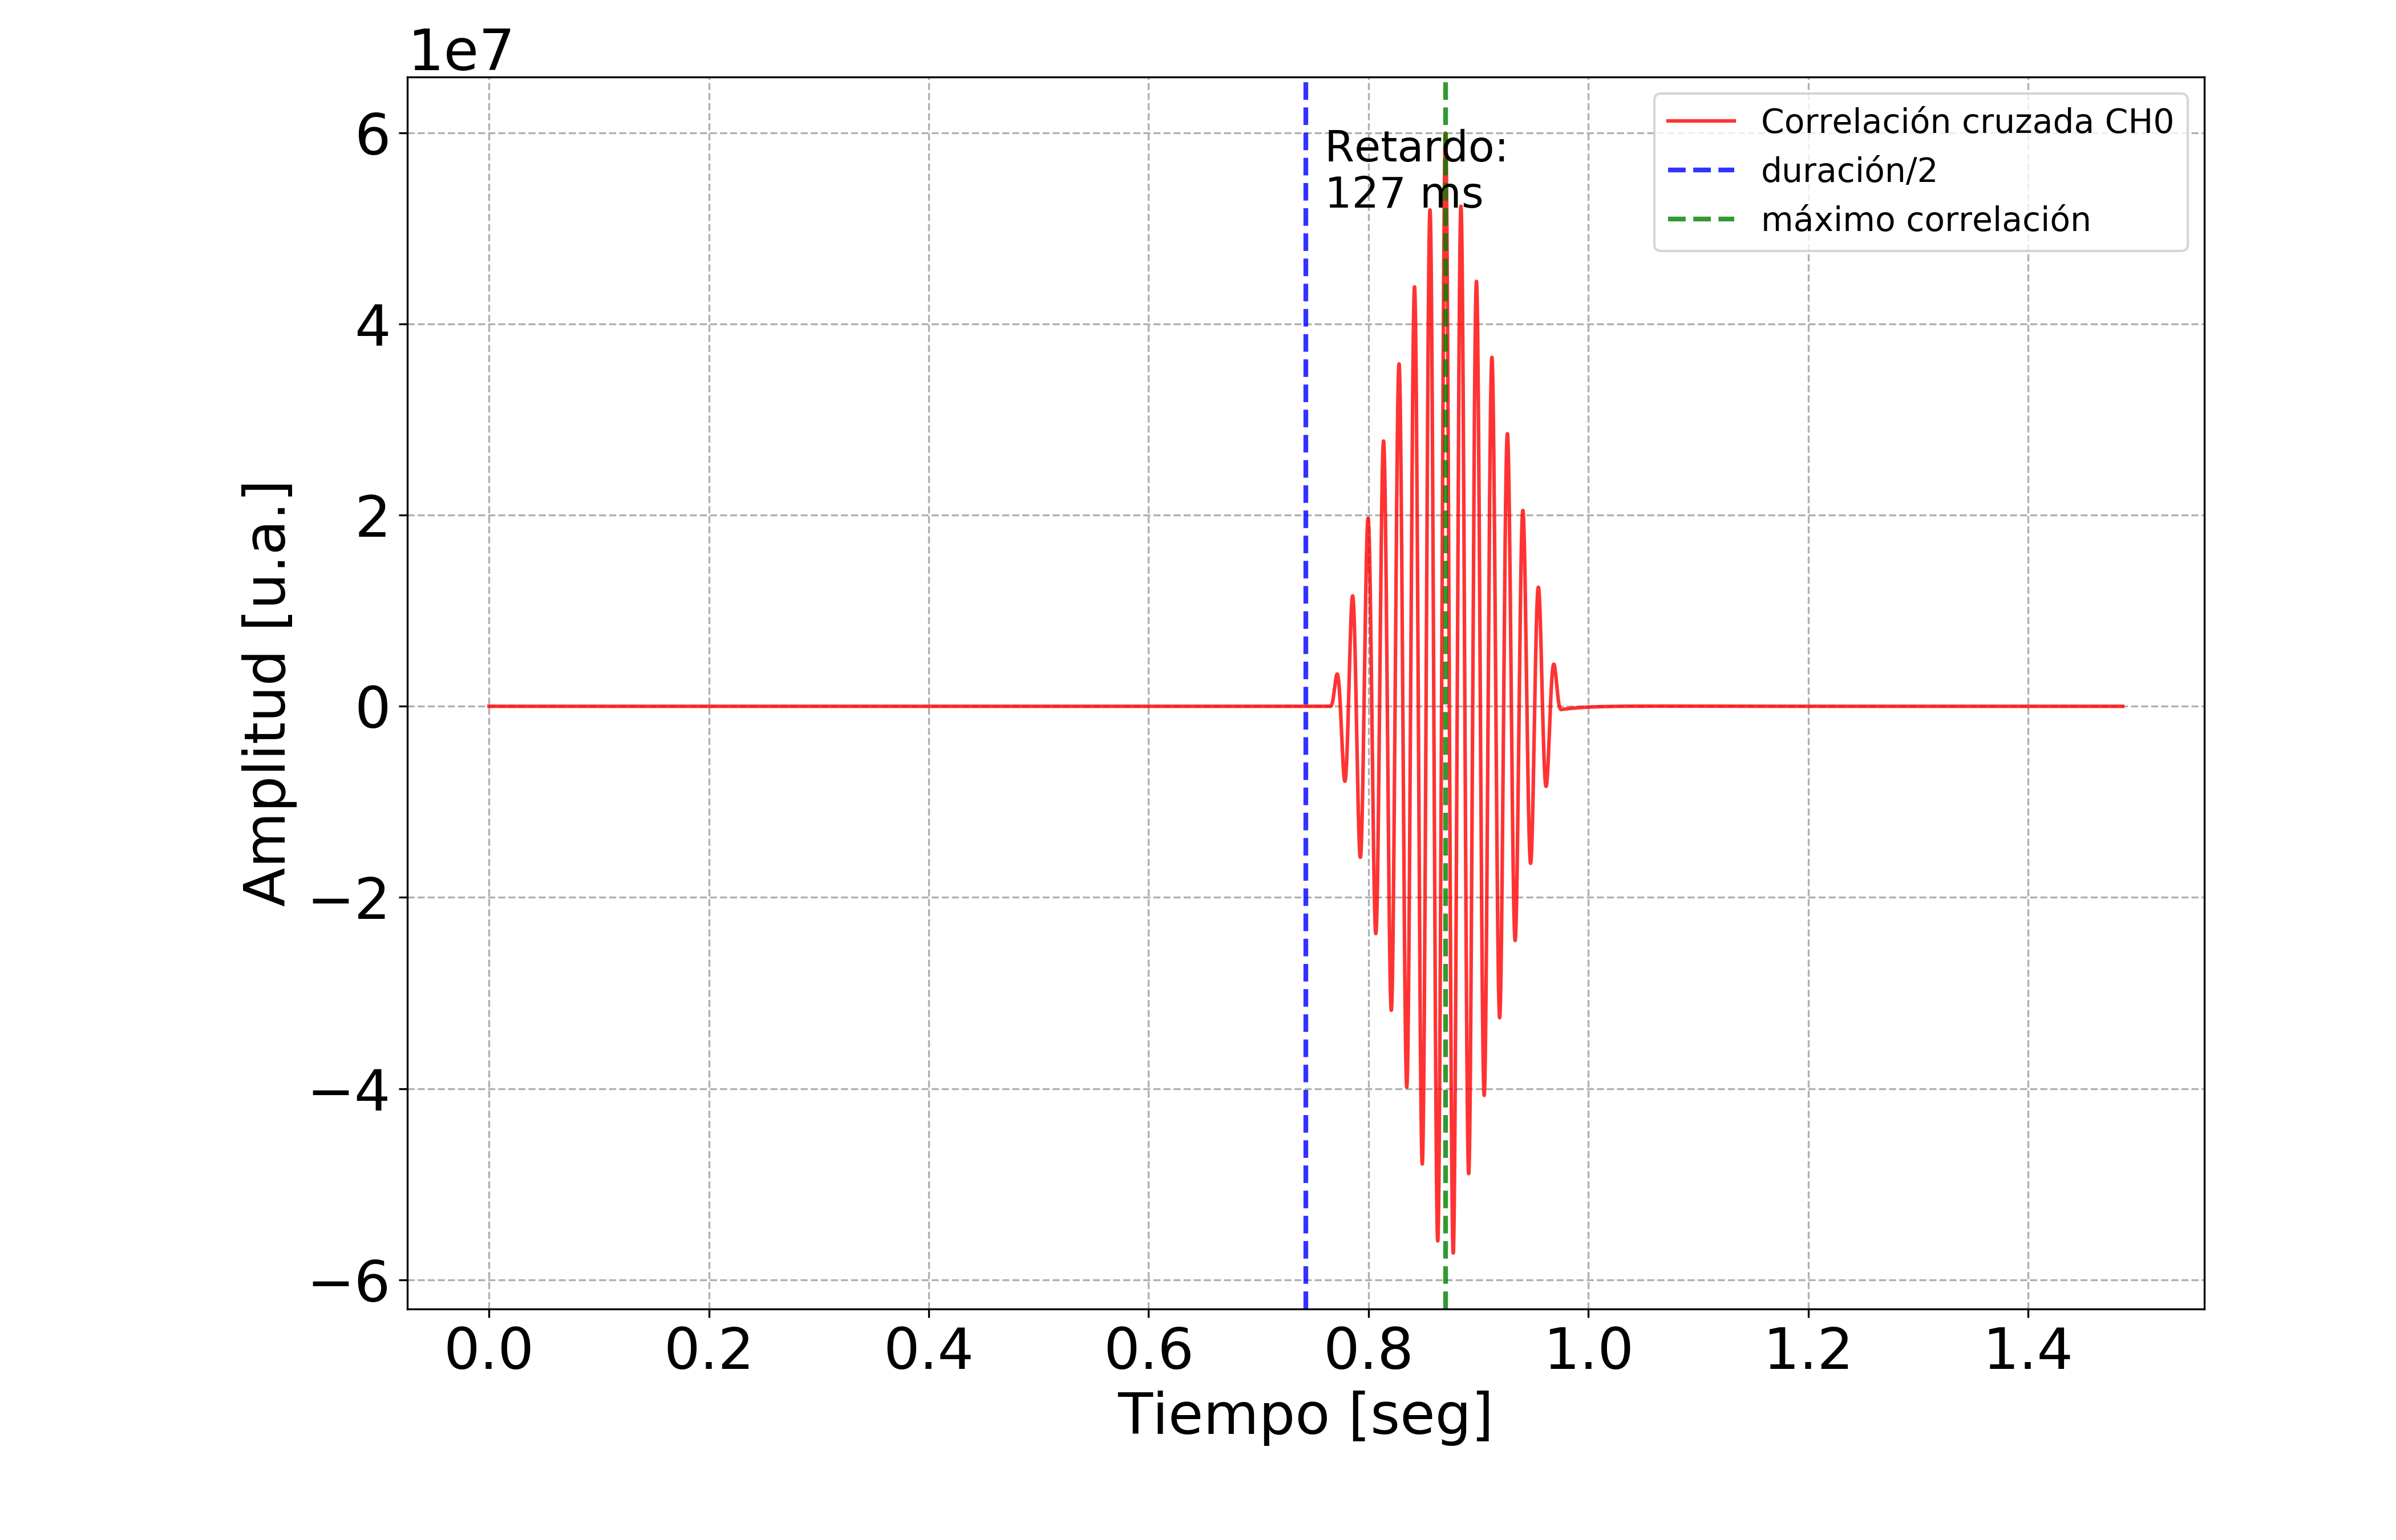
\includegraphics[scale=0.45]{correlacion_cruzada.png}
\caption{Correlación cruzada de la señal sintética del canal CH0 y la señal adquirida en el canal CH0.\label{fig:correlacion_cruzada}}
\end{figure} 

En la Figura \ref{fig:senal_adquirida_corregida} se muestra la señal adquirida luego de eliminar el retardo y recortando la señal a la misma duración de la señal de digital enviada. De esta manera la señal digital y la señal adquirida tienen la misma duración y la misma cantidad de muestras.
 
\begin{figure} [H]
\centering
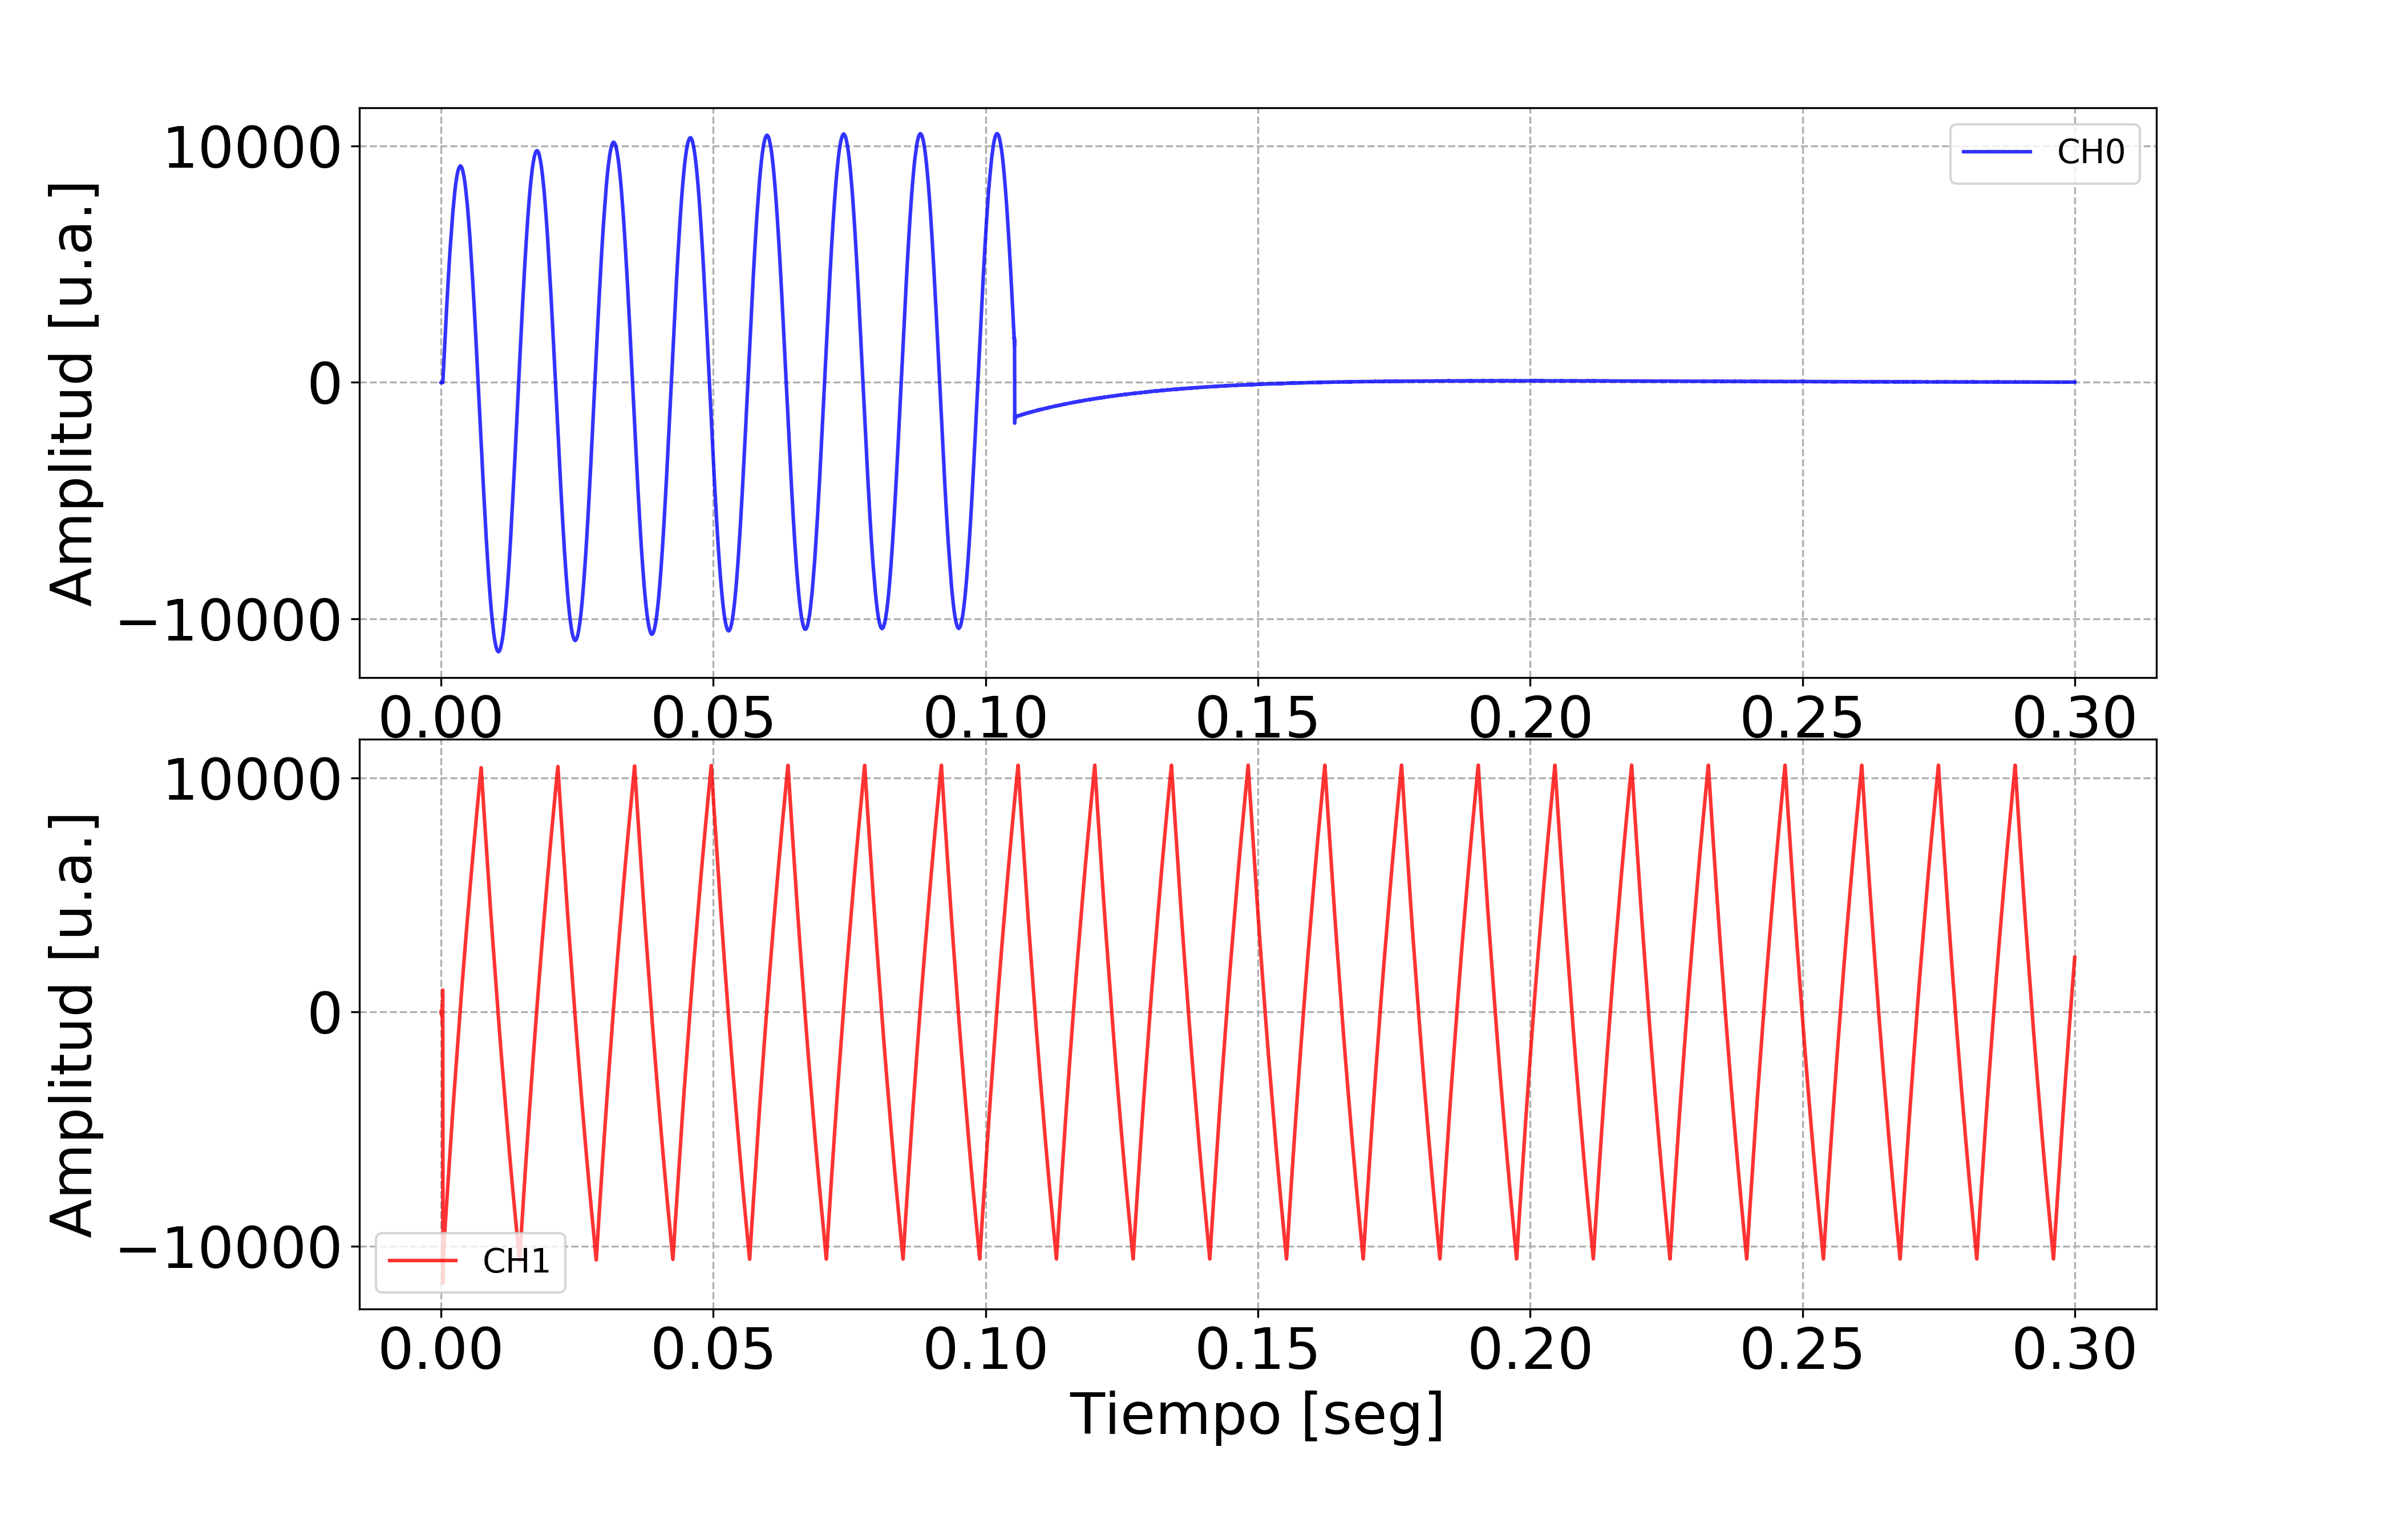
\includegraphics[scale=0.45]{senal_adquirida_corregida.png}
\caption{Señal adquirida corregida en los canales CH0 y CH1. \label{fig:senal_adquirida_corregida}}
\end{figure} 
 

\subsection*{Retardo}
A continuación nos propusimos realizar un estudio estadístico del retardo entre las señales de entrada y salida, en función del tamaño de buffer de salida, el buffer de entrada y la frecuencia de sampleo. Para cada caso distinto se realizó un barrido de diez pasos o corridas iguales enviando un seno de 1000 Hz en ambos canales. En la Figura \ref{fig:frec_0} se muestra el retardo en función del número de corrida, para distintos tamaños de buffer de entrada y salida. Se observa que el retardo es mayor en la primera medición de cada barrido, y que luego se mantiene estable alrededor de los 100 ms. Después de la primera corrida, se observa un leve aumento del retardo a medida que el tamaño o duración de la señal se achica, y se observa que a mismo tamaño de buffer de entrada la variabilidad del retardo es pequeña. Similares resultados se observan en el caso en que se aumenta la frecuencia de sampleo (Figura \ref{fig:frec_7}). 
Tampoco se observa dependencia del retardo con la señal enviada. En la Figura \ref{fig:frec} se muestra el retardo al variar la frecuencia del seno enviado, para mismo tamaño de buffer de entrada, salida y frecuencia de sampleo.
 
\begin{figure} [H]
\centering
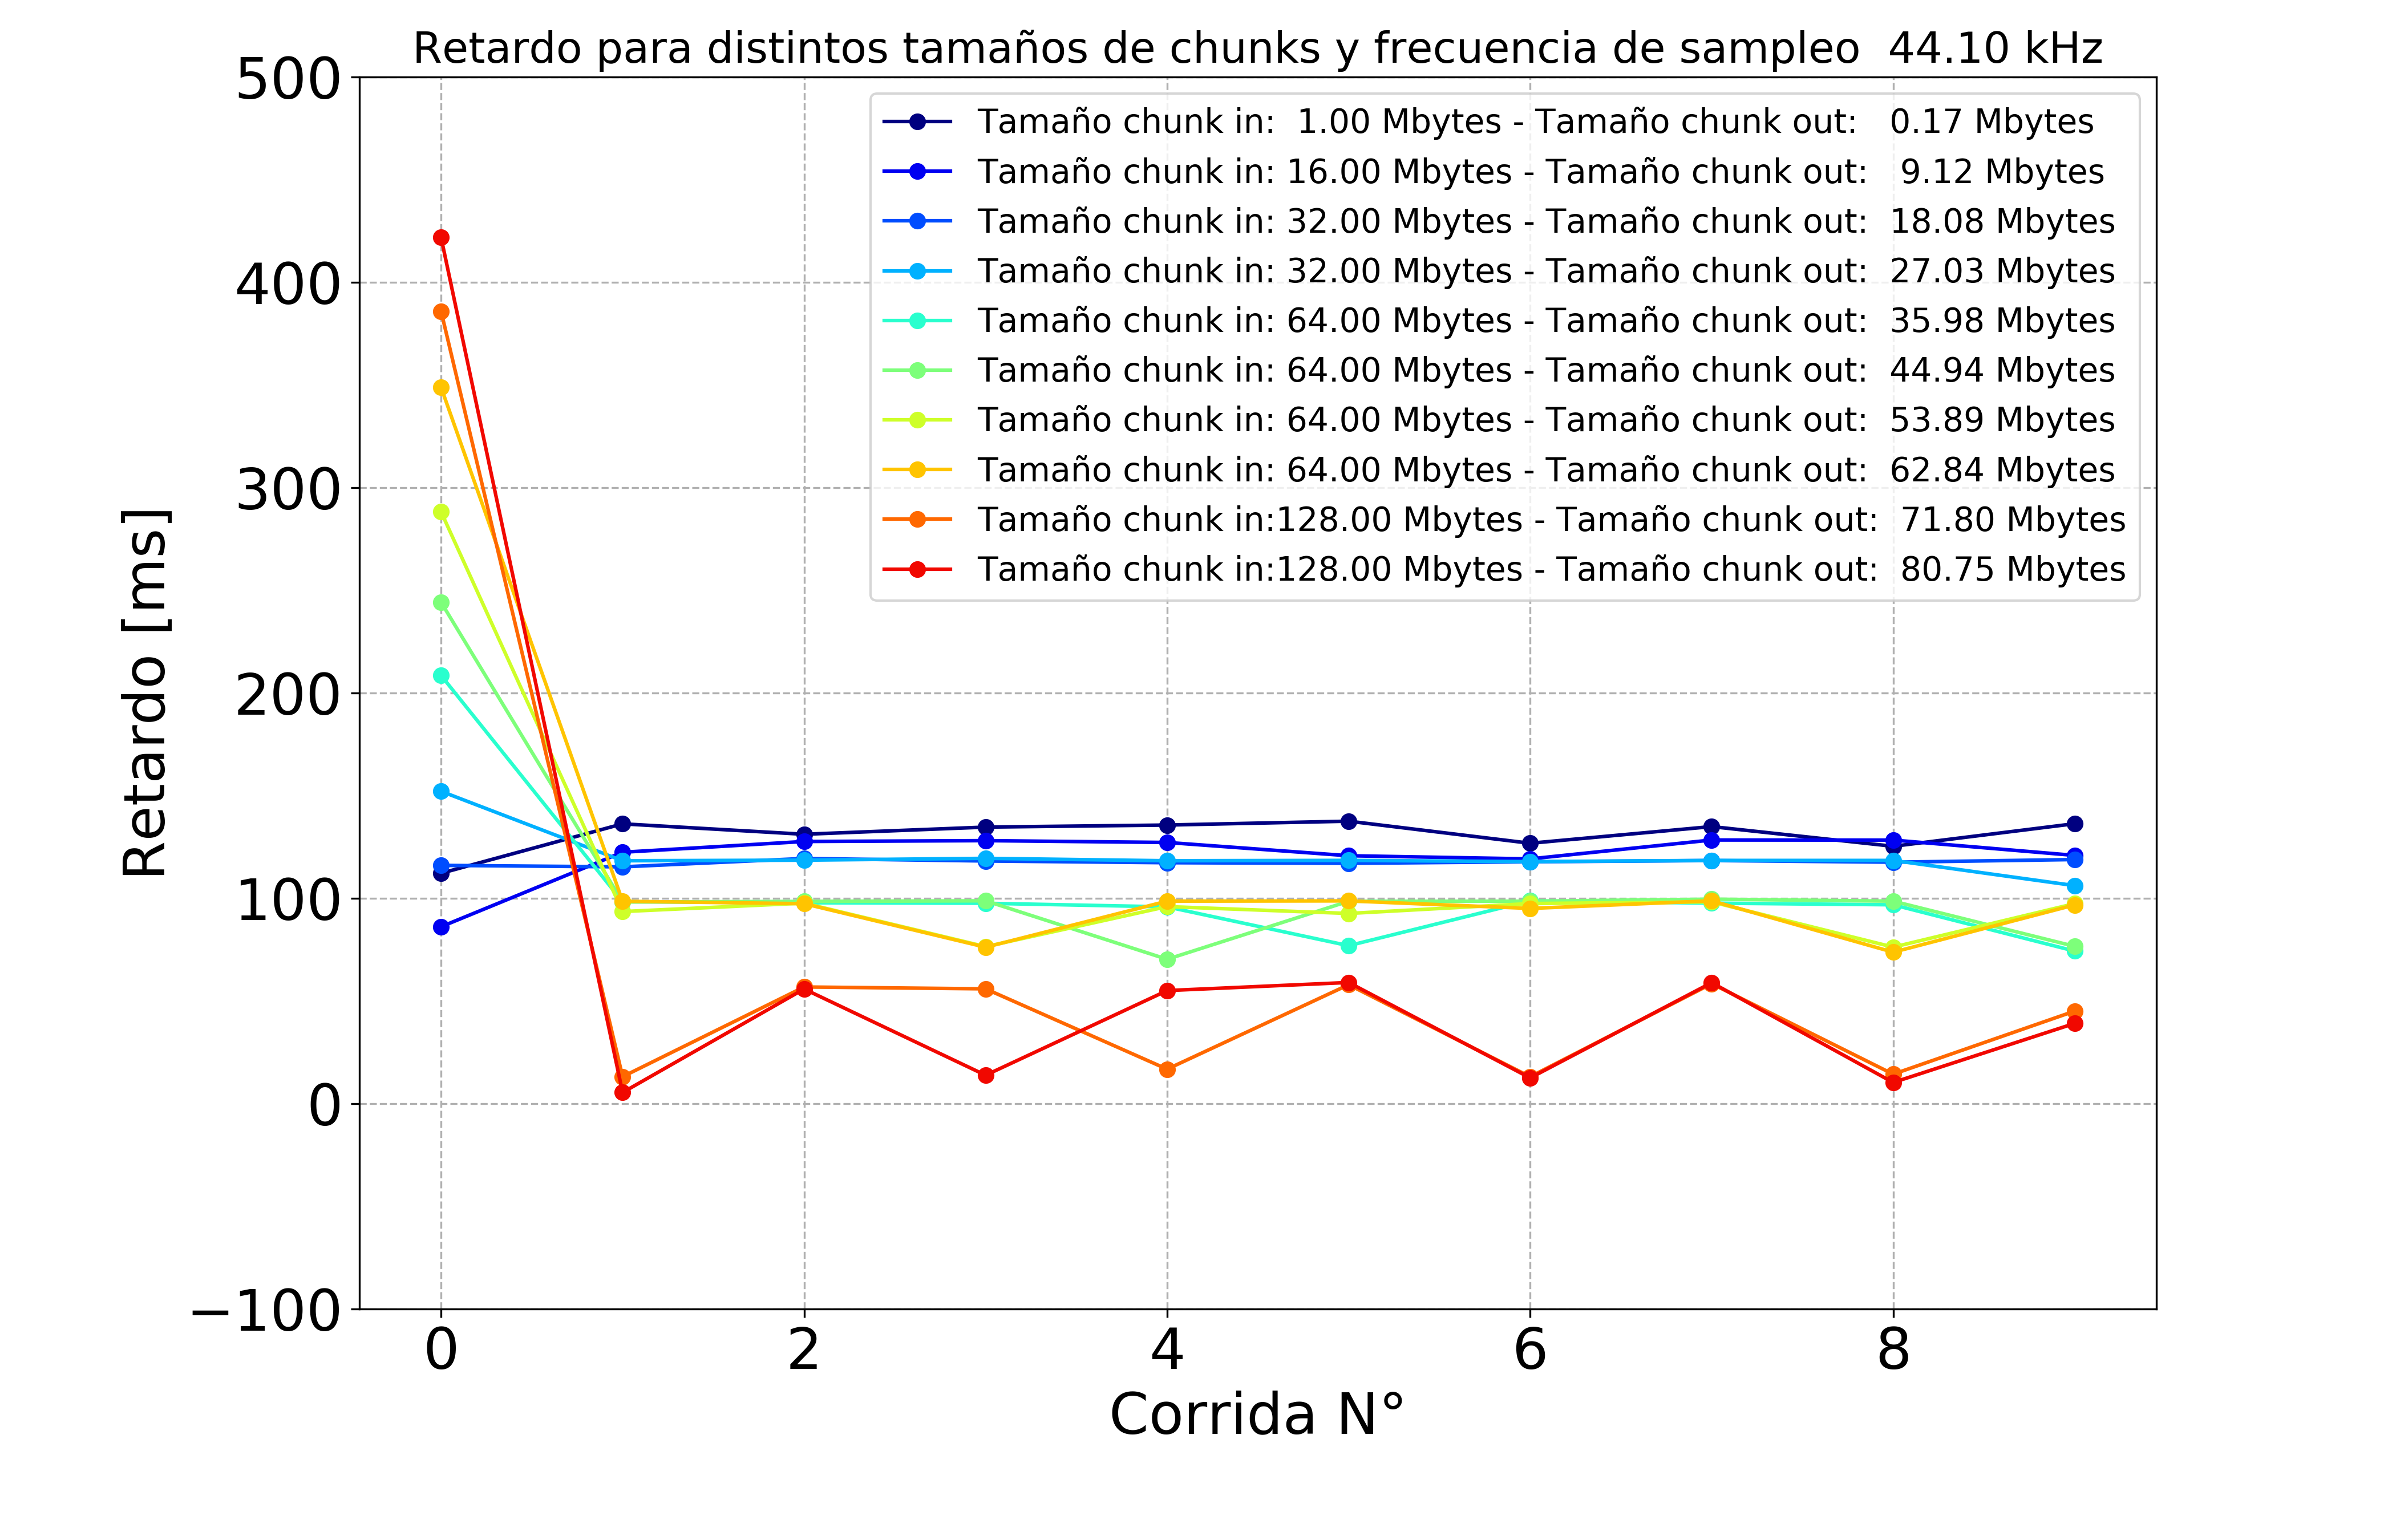
\includegraphics[scale=0.45]{frec_0.png}
\caption{Retardo entre la señal enviada y adquirida en función del número de corrida y para distintos tamaños de buffer. Frecuencia de sampleo de 44.1 kHz. \label{fig:frec_0}}
\end{figure} 
 
\begin{figure} [H]
\centering
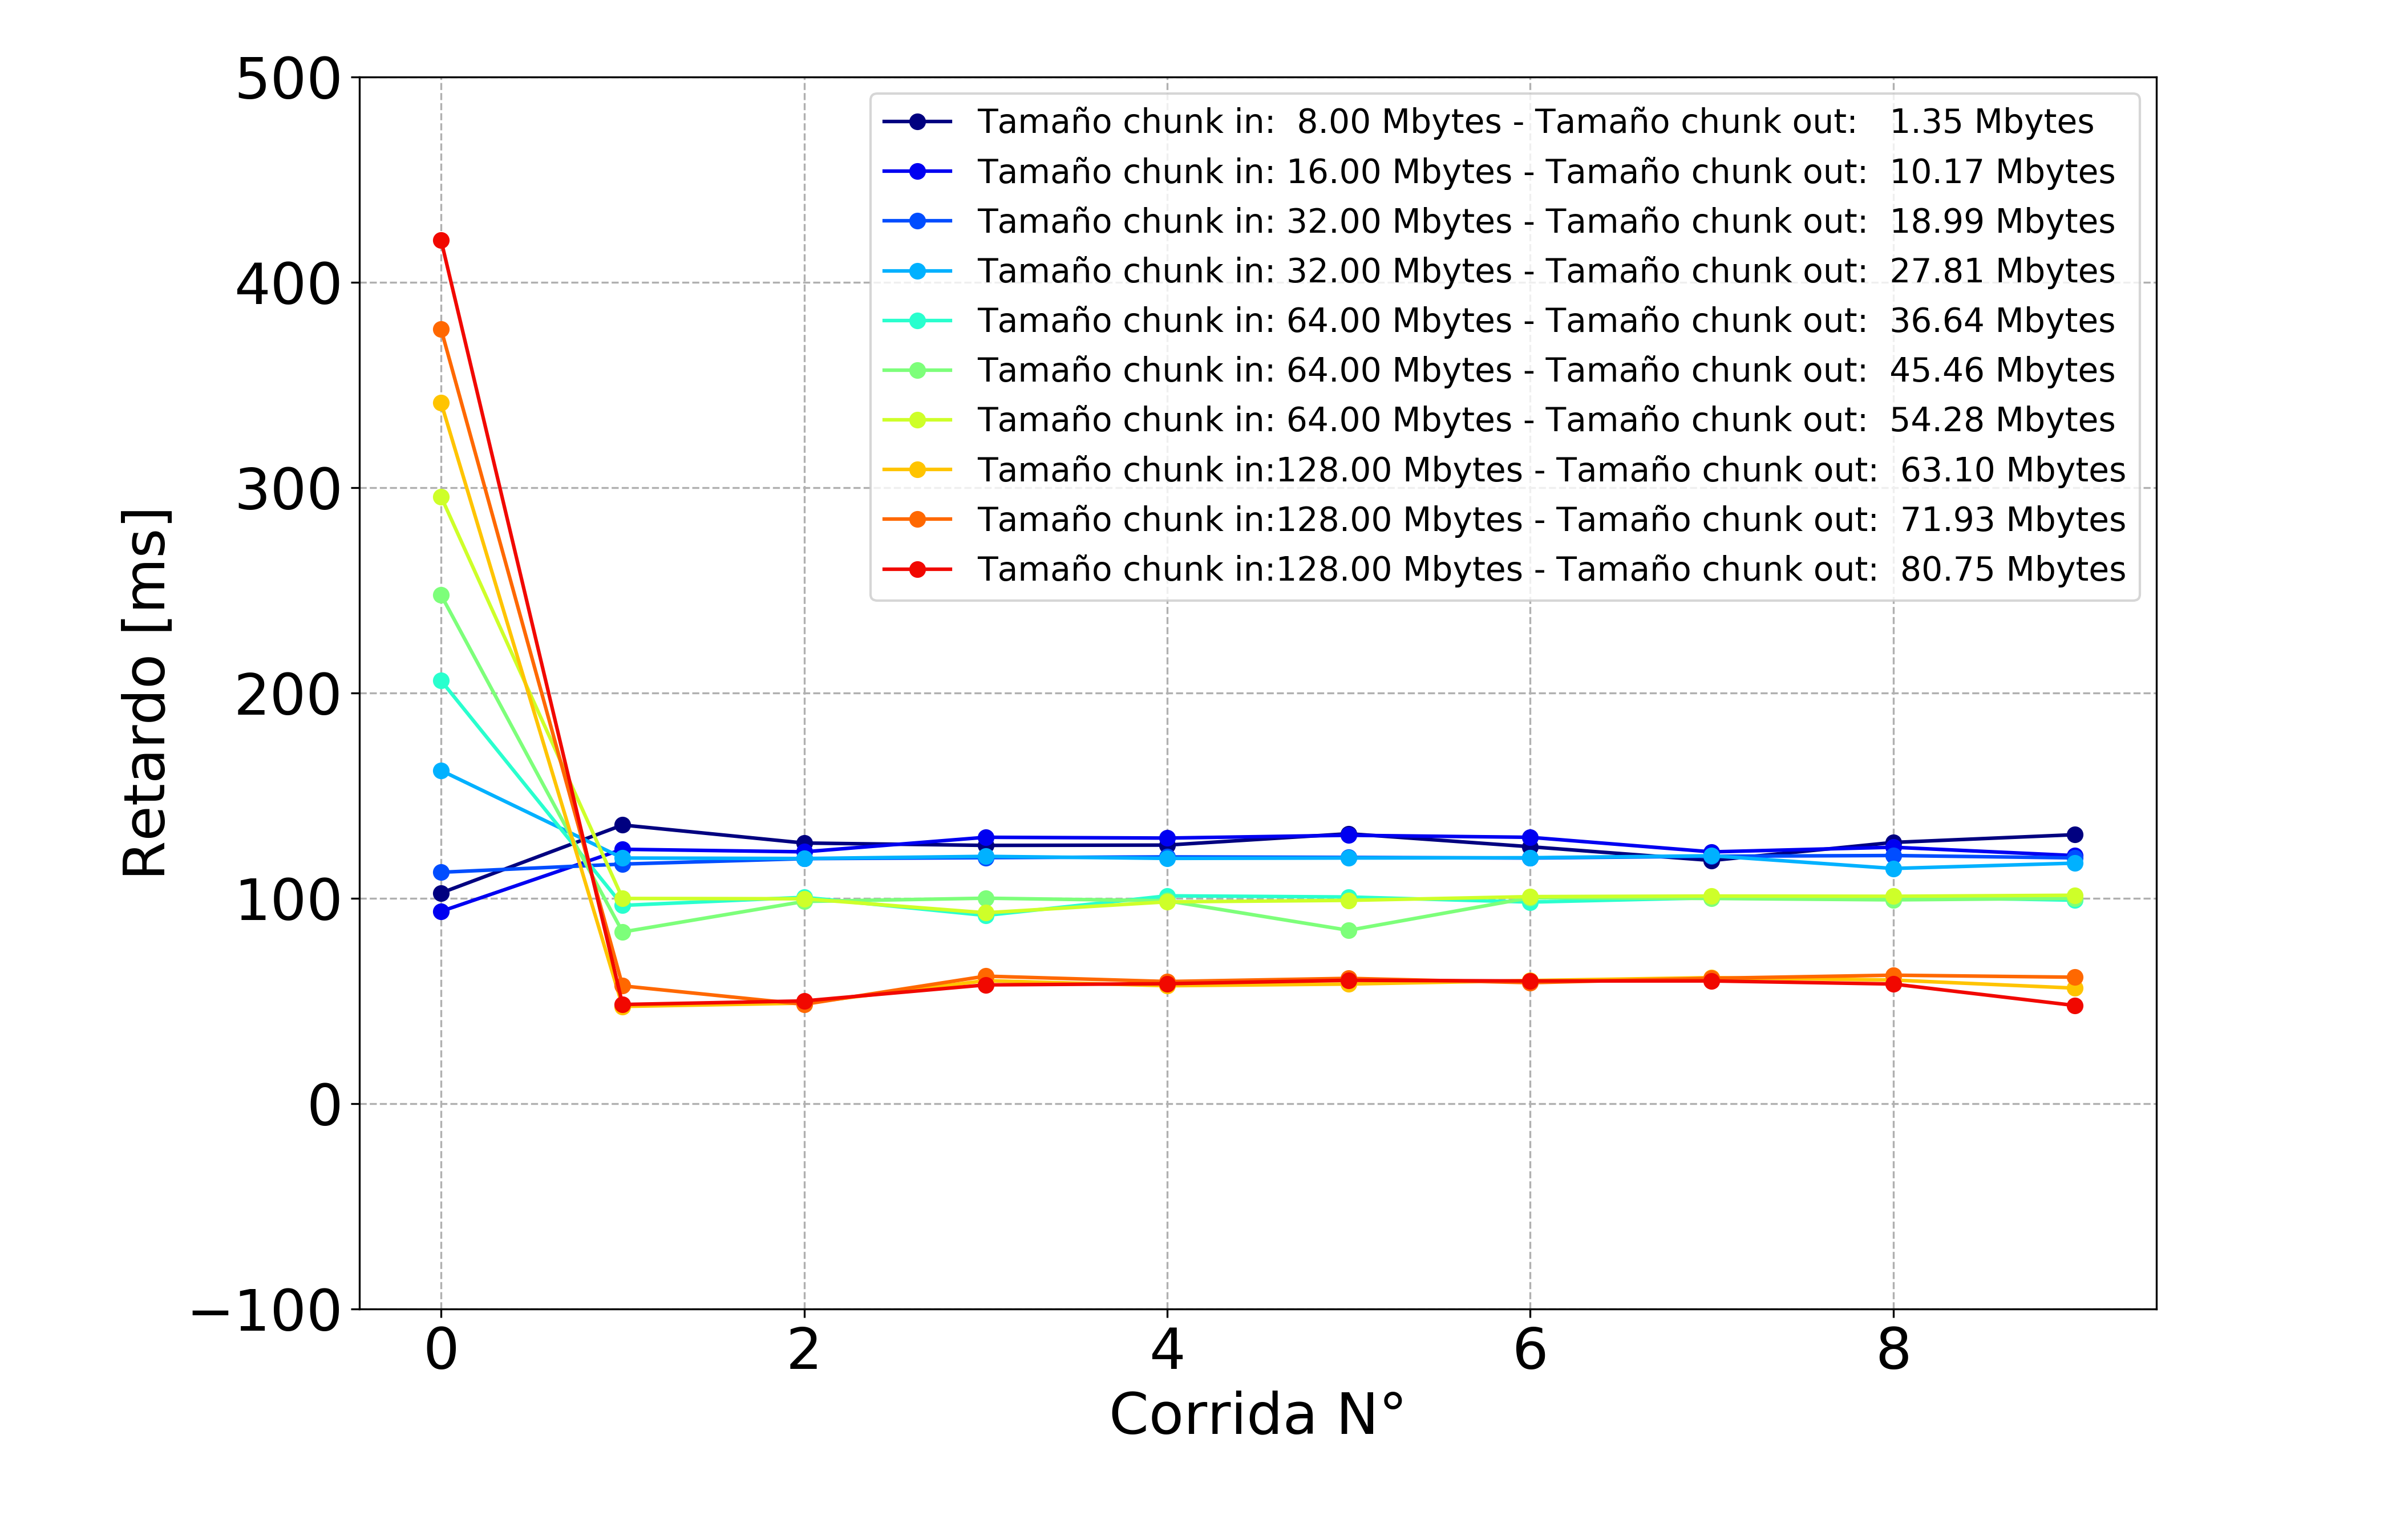
\includegraphics[scale=0.45]{frec_7.png}
\caption{Retardo entre la señal enviada y adquirida en función del número de corrida y para distintos tamaños de buffer. Frecuencia de sampleo de 352.8 kHz.  \label{fig:frec_7}}
\end{figure} 




\begin{figure} [H]
\centering
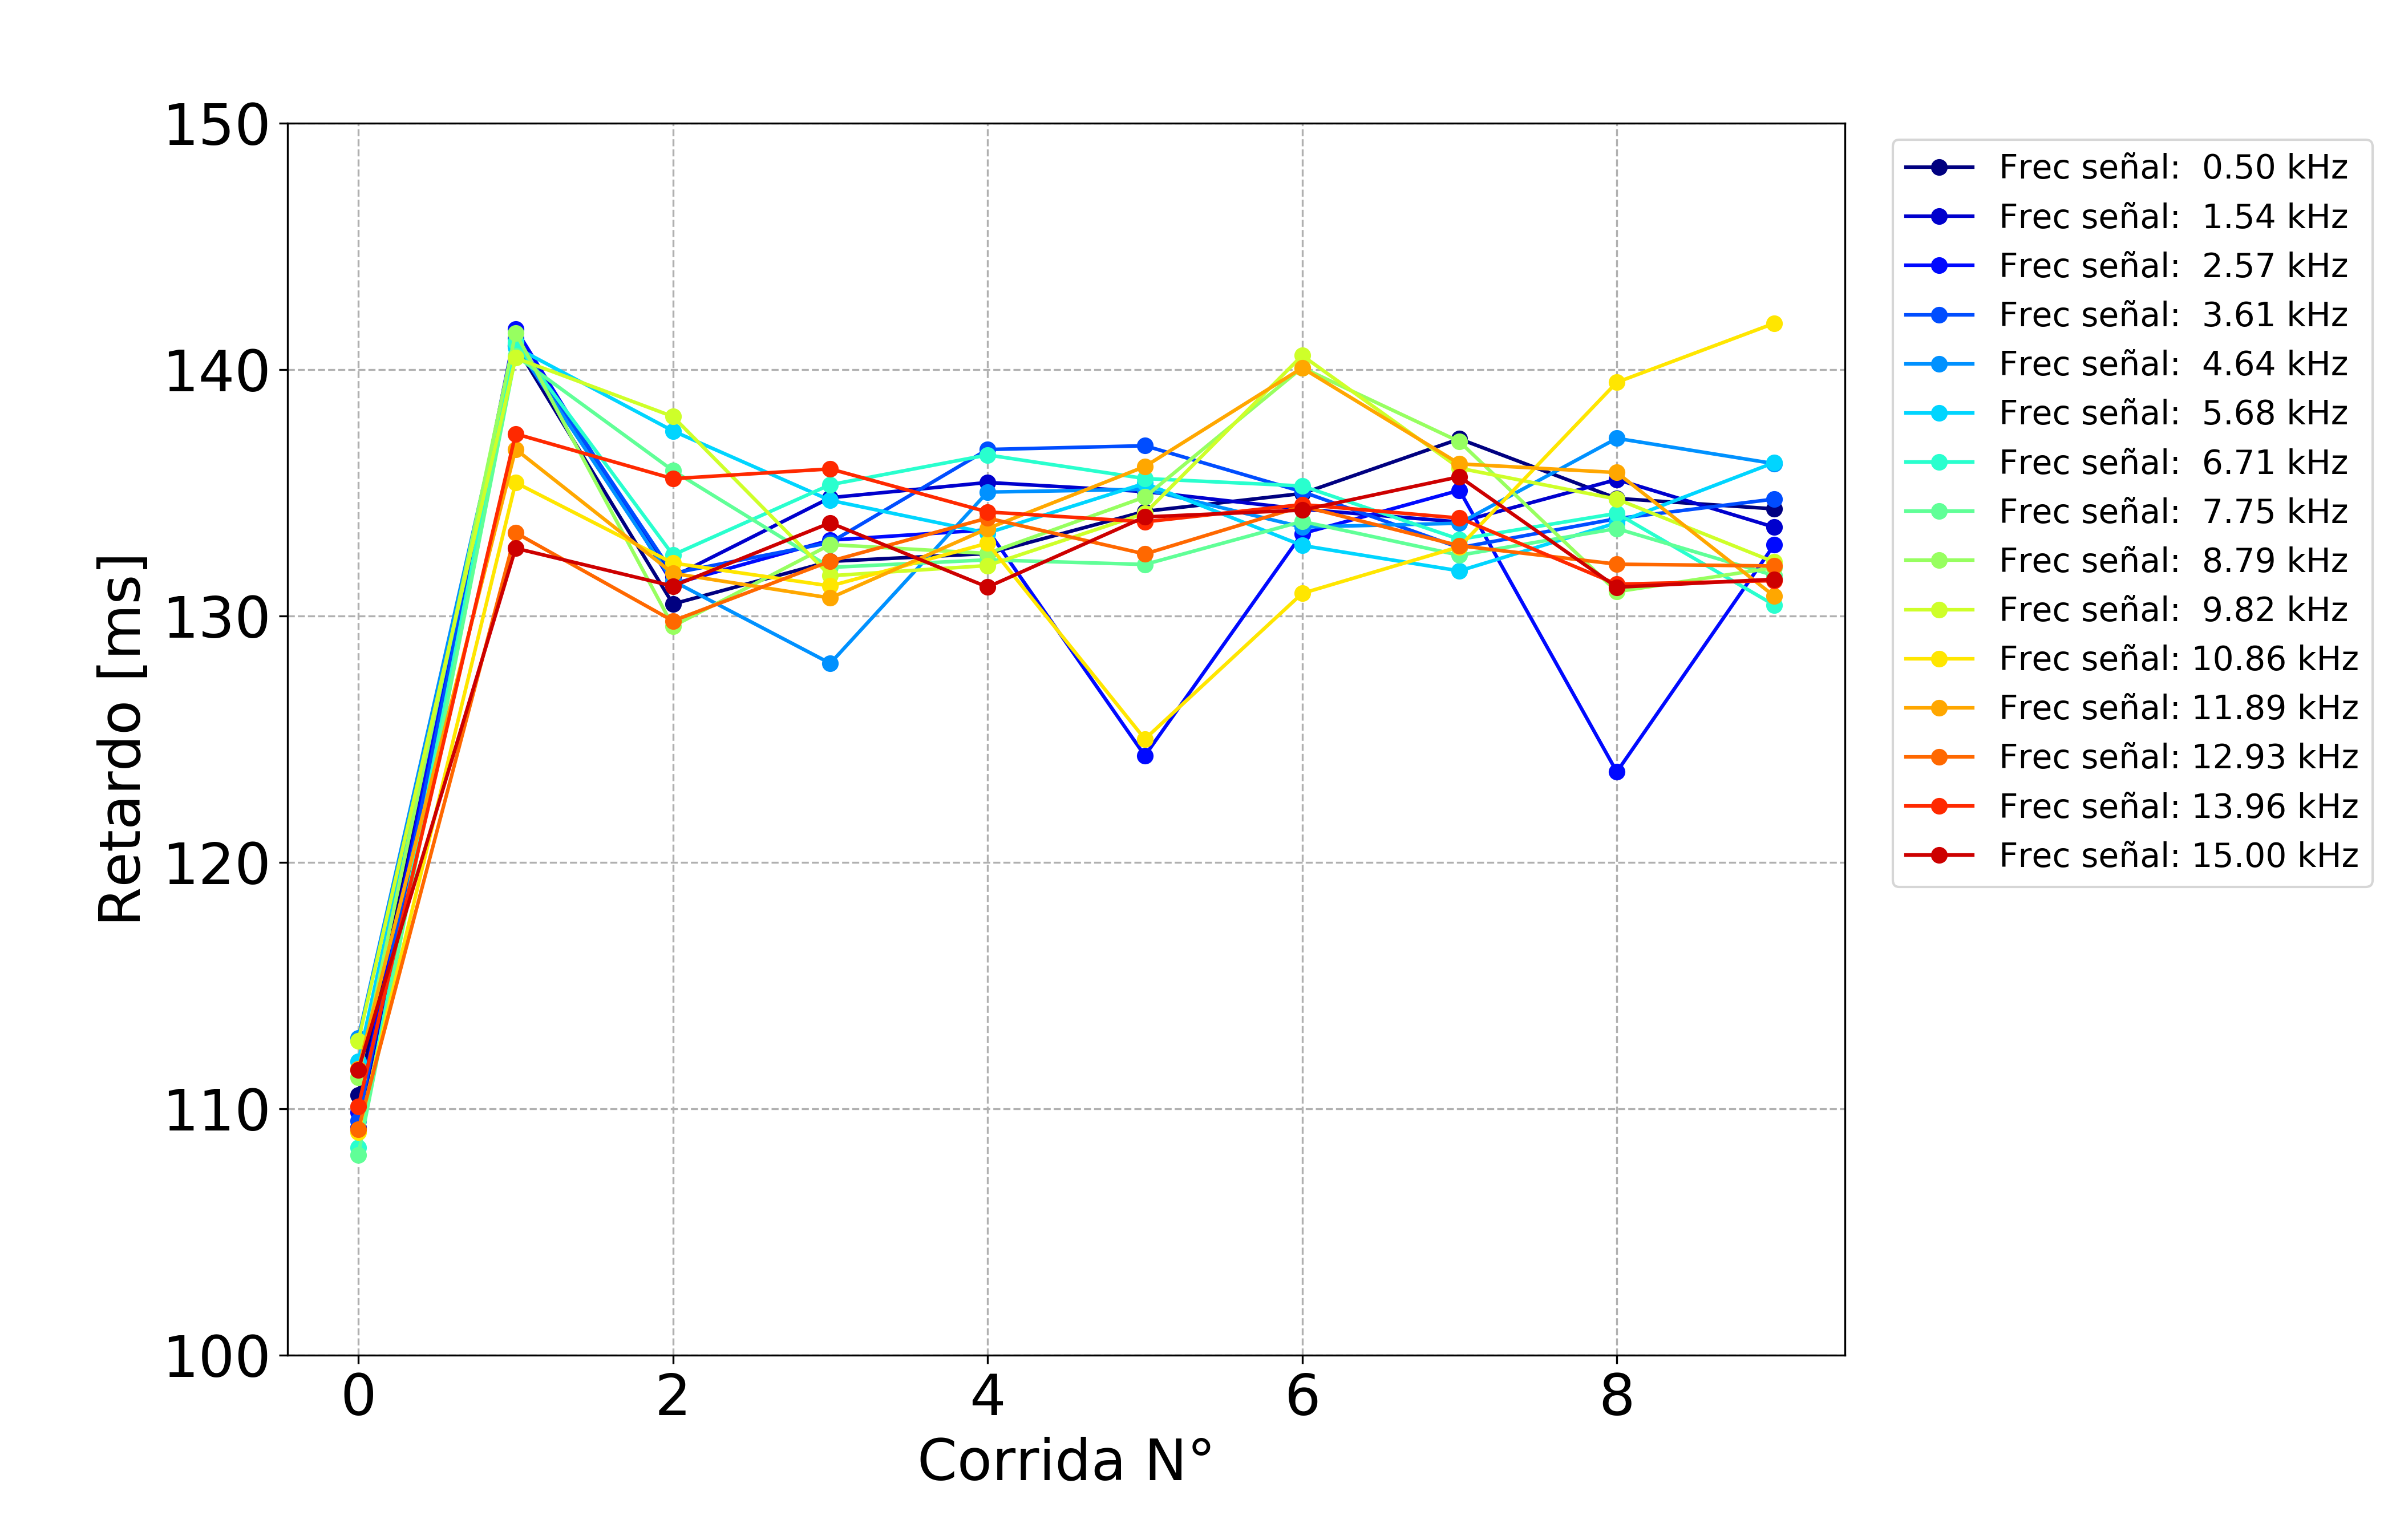
\includegraphics[scale=0.45]{frec.png}
\caption{Retardo entre la señal enviada y adquirida en función del número de corrida y para distintas frecuencias de señales enviadas. Frecuencia de sampleo de 176.4 kHz.  \label{fig:frec}}
\end{figure} 






% to comment sections out, use the command \ifx and \fi. Use this technique when writing your pre lab. For example, to comment something out I would do:
%  \ifx
%	\begin{itemize}
%		\item item1
%		\item item2
%	\end{itemize}	
%  \fi

%
\end{document}


   \begin{figure}
        \begin{subfigure}[b]{0.5\textwidth}
                \centering
                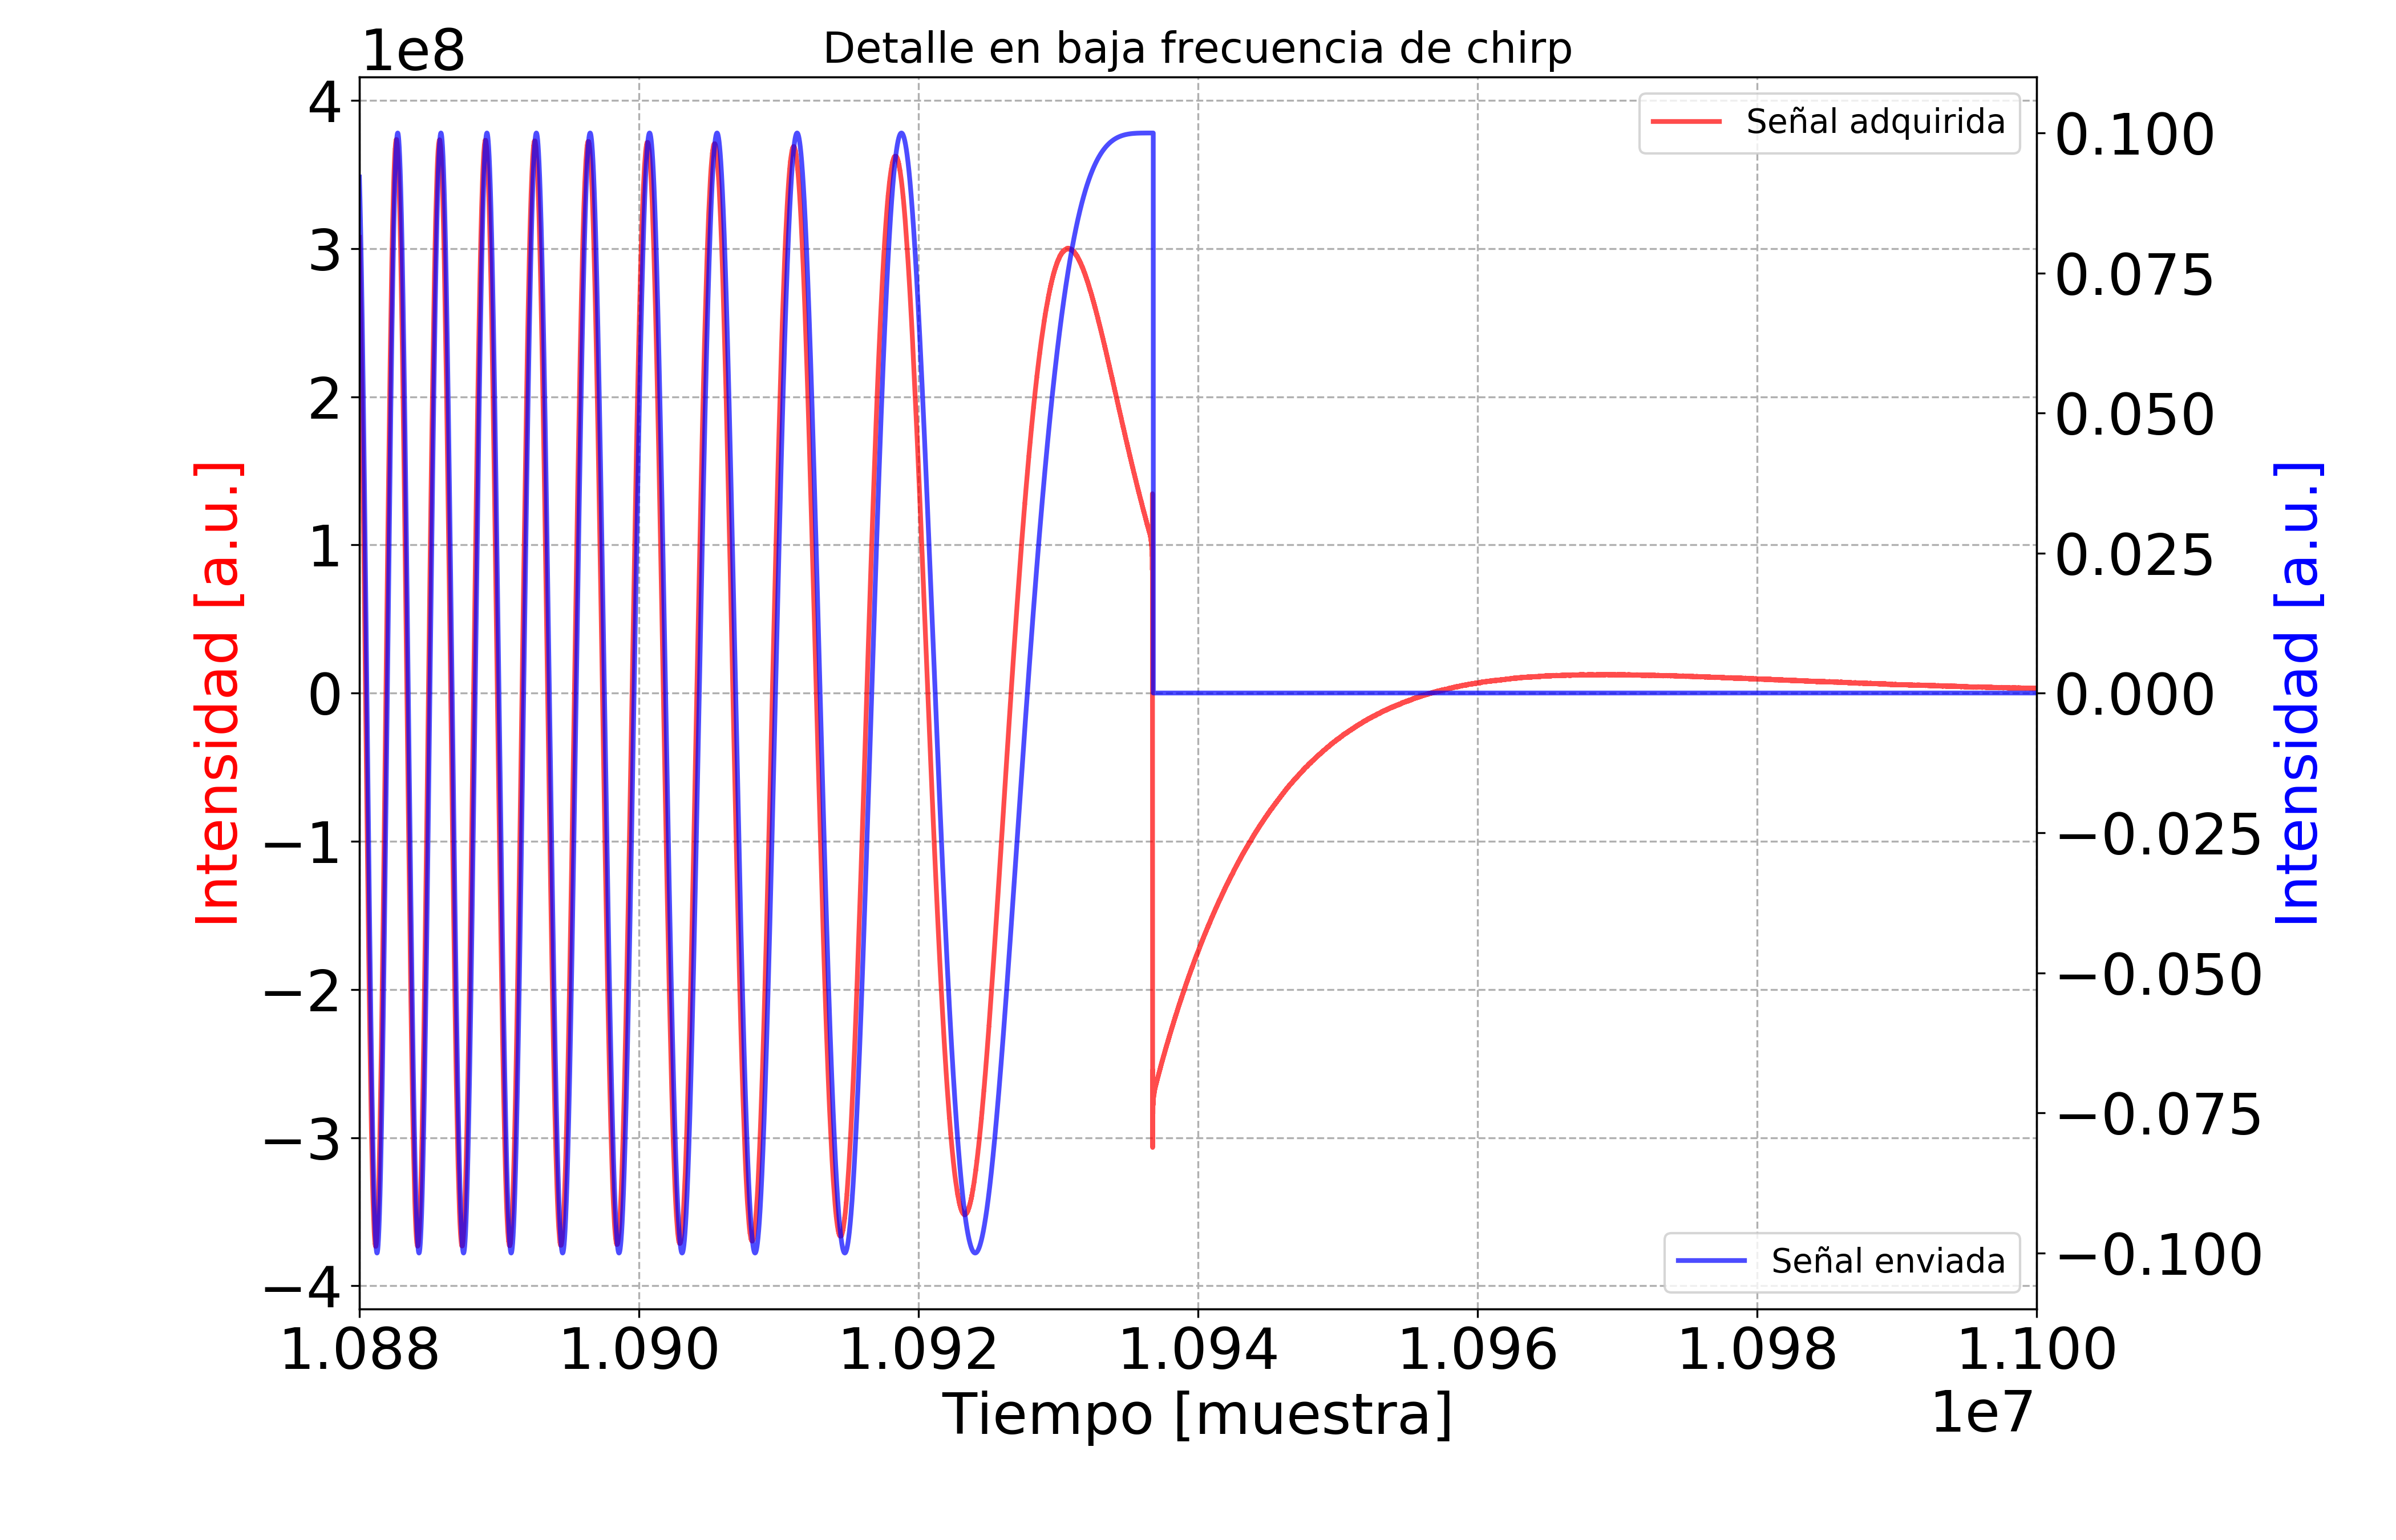
\includegraphics[width=\linewidth]{chirp_baja_tiempo.png}
                \caption{} \label{fig:chirpbaja}
        \end{subfigure}%
        \begin{subfigure}[b]{0.5\textwidth}
                \centering
                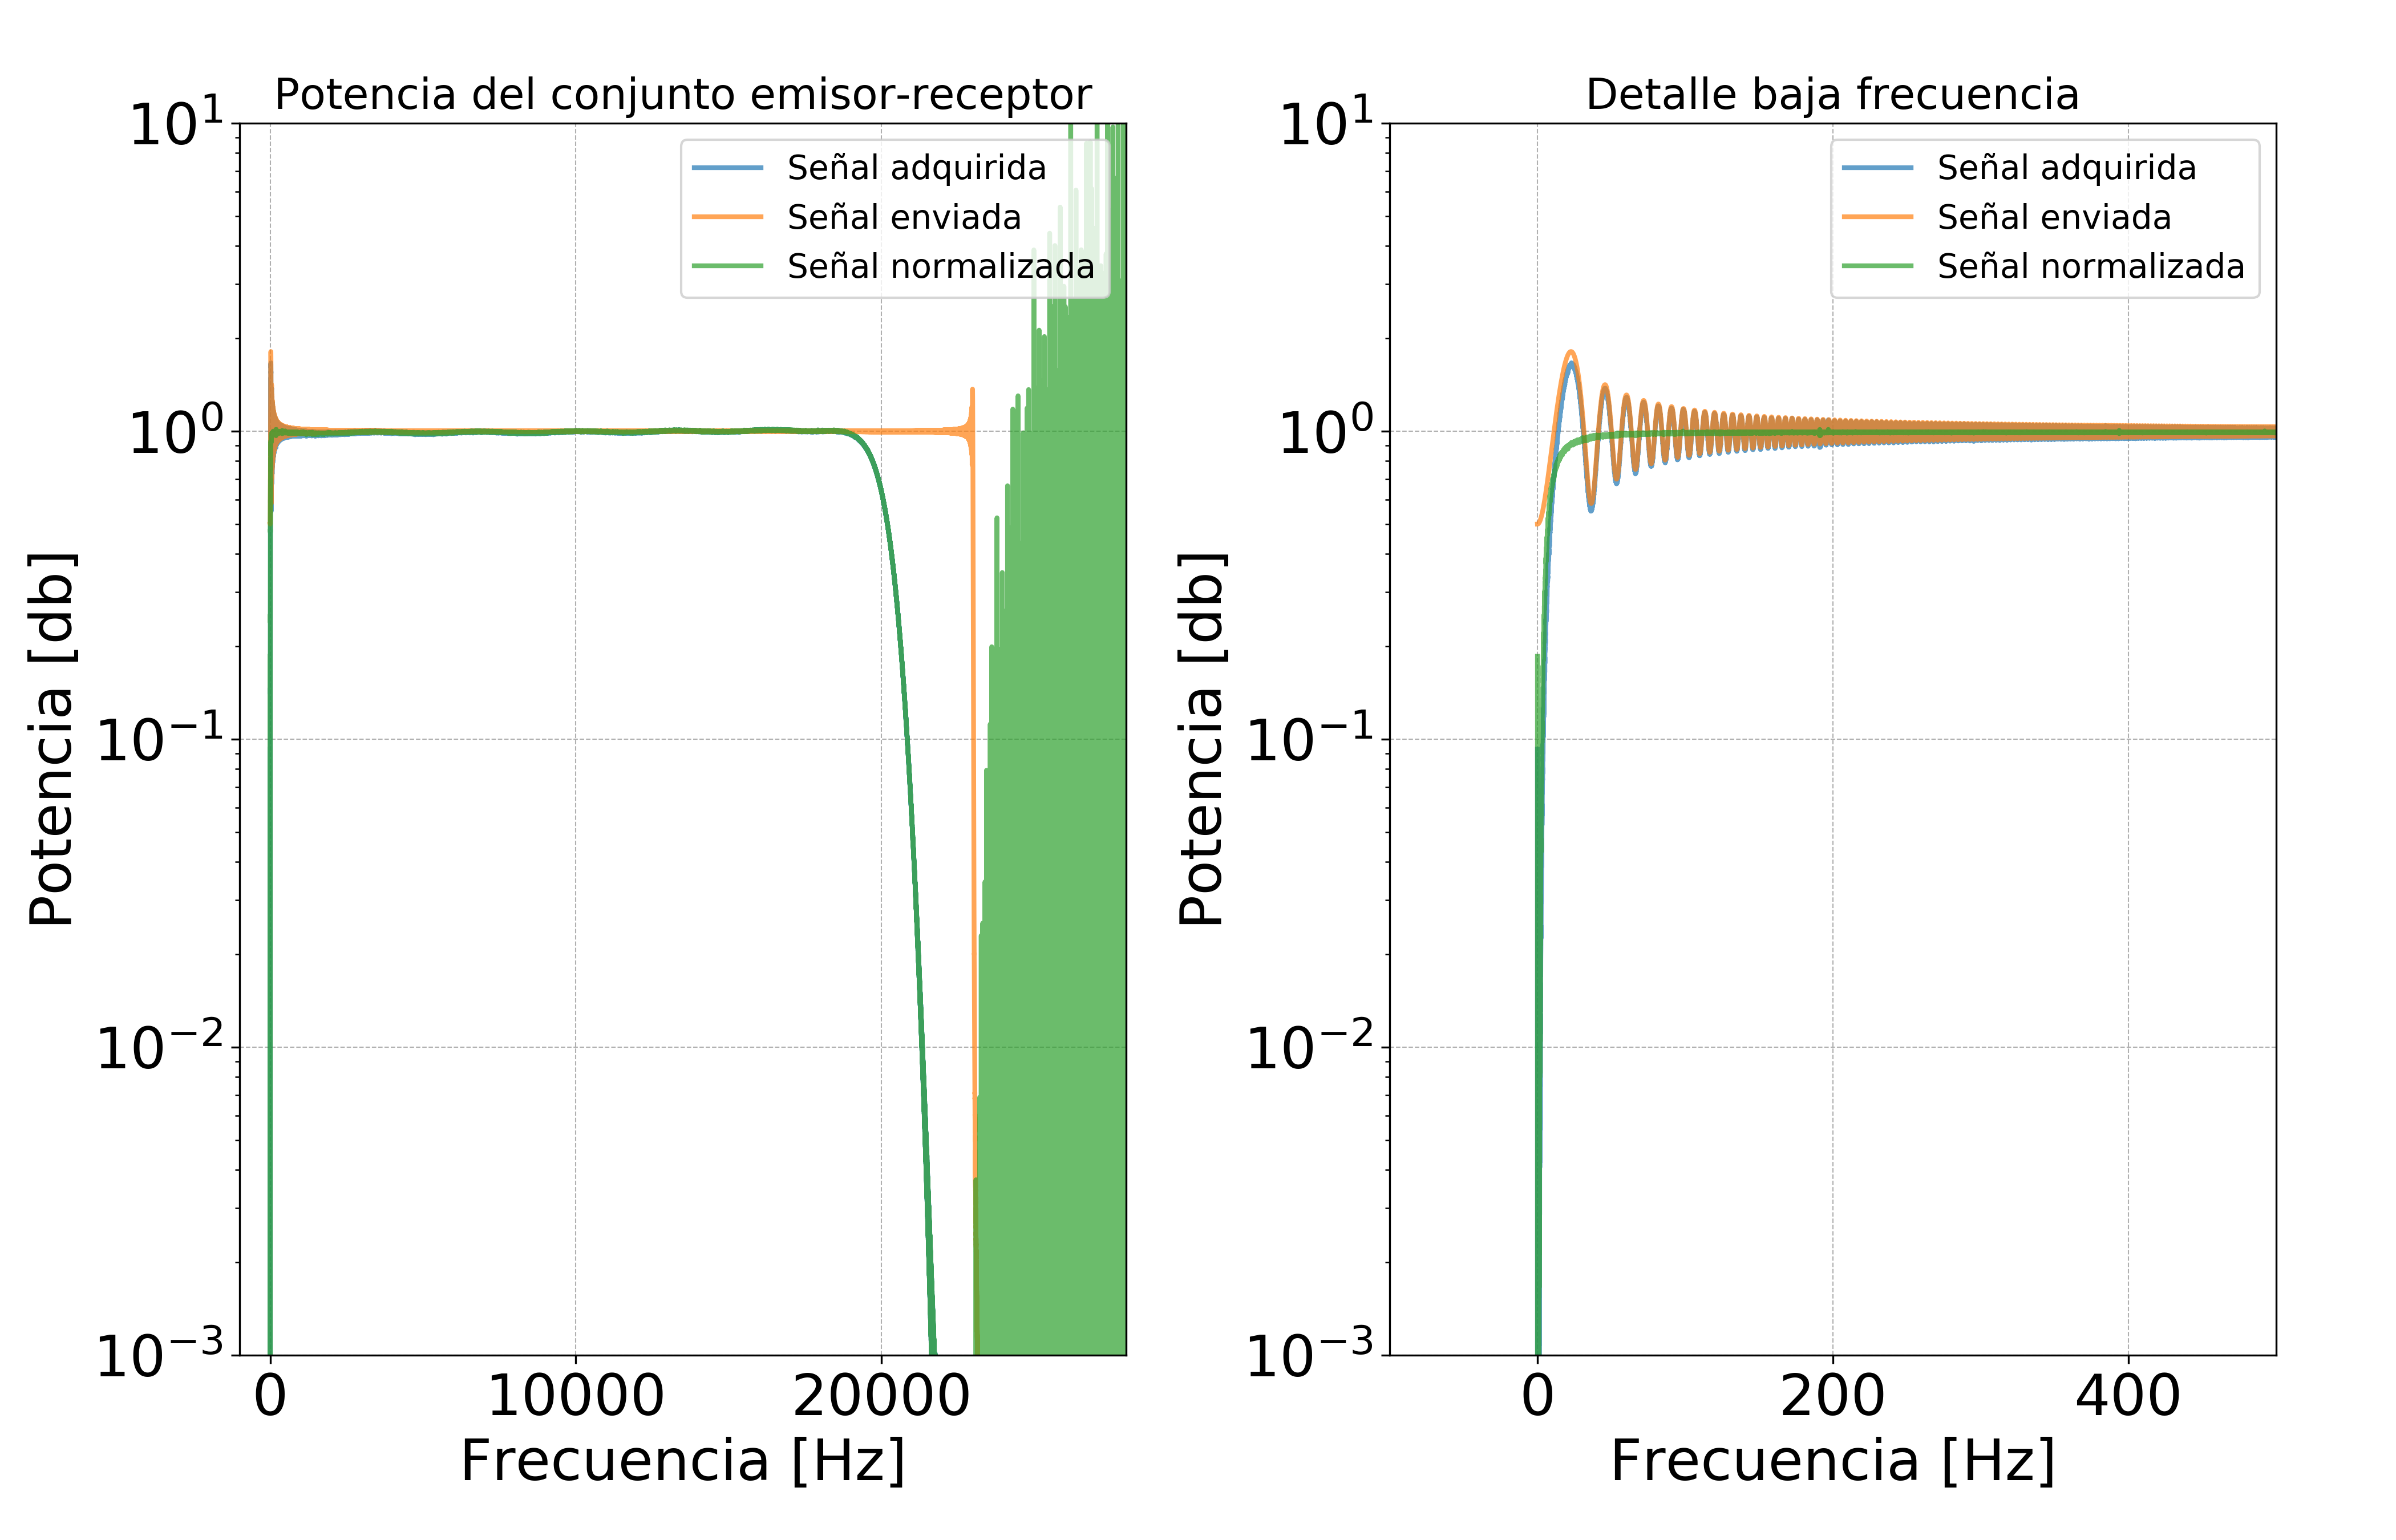
\includegraphics[width=\linewidth]{chirp_detalle.png}
                \caption{} \label{fig:chirpdetalle}
        \end{subfigure}%
        \caption{a) b) Detalle del ripple al inicio de la señal}\label{fig:chirp}
\end{figure}
